\documentclass[10pt,fleqn]{report}

\setcounter{tocdepth}{3}
\setcounter{secnumdepth}{3}

\usepackage{a4}
\usepackage{latexsym}
\usepackage{epsf}
\usepackage{listings}
\usepackage{xcolor}
\usepackage{titlesec}
\usepackage{lipsum}
\usepackage{scrextend}
\usepackage{tikz}
\usetikzlibrary{fit}
\usetikzlibrary{calc}
\usetikzlibrary{positioning}
\usetikzlibrary{shadows}
\usetikzlibrary{shadows.blur}
\usetikzlibrary{shapes.symbols}
\usepackage{fontspec}
\usepackage{wrapfig}
\usepackage{nameref}
\usepackage{hyperref}
\usepackage{enumitem}
\usepackage{relsize}
\usepackage{pdfpages}
\usepackage{makeidx}
\usepackage{csquotes}

\usepackage{amsmath, amsthm, amssymb}
\usepackage[ngerman, english]{babel}
\usepackage{marvosym}
\usepackage{graphics}
\usepackage{extarrows}
\usepackage{forloop}
\usepackage{mathtools}

\usepackage[]{algorithm2e}

\usepackage{hyperref}% http://ctan.org/pkg/hyperref
\usepackage{cleveref}% http://ctan.org/pkg/cleveref
\usepackage{lipsum}% http://ctan.org/pkg/lipsum
\newtheorem{definition}{Definition}
\newtheorem{theorem}{Theorem}
\newtheorem{lemma}{Lemma}
\newtheorem{preliminary}{Preliminary}
\newtheorem{notation}{Notation}
\newtheorem{property}{Property}
\newtheorem{corollary}{Corollary}
\newtheorem{example}{Example}
\newtheorem{hypothesis}{Hypothesis}

\crefname{theorem}{Theorem}{Theorems}
\crefname{definition}{Definition}{Definitions}
\crefname{lemma}{Lemma}{Lemmas}
\crefname{preliminary}{Preliminary}{Preliminaries}
\crefname{notation}{Notation}{Notations}
\crefname{property}{Property}{Properties}
\crefname{corollary}{Corollary}{Corollaries}
\crefname{example}{Example}{Examples}
\crefname{hypothesis}{Hypothesis}{Hypotheses}


\newenvironment{beweis}{\begin{proof}[Beweis]}{\end{proof}}


\usepackage[font=footnotesize,labelfont=bf]{caption}

\newfontfamily\sansfont[Extension = .ttf, Path = ./fonts/, UprightFont = OpenSans-Regular, BoldFont=OpenSans-SemiBold, ItalicFont=OpenSans-SemiBold]{OpenSans}


\titleformat{\chapter}[display]
  {\sansfont\bfseries}{}{0pt}{\huge}
  
\renewcommand{\contentsname}{\sansfont Content}  

\definecolor{folderbg}{RGB}{70, 130, 180}
\definecolor{folderborder}{RGB}{50,50,50}
\definecolor{DarkGreen}{RGB}{0, 136, 0}
\newlength\Size
\setlength\Size{5pt}


\pgfdeclarelayer{bg}
\pgfsetlayers{bg,main}

\renewcommand{\textfraction}{0.05}
\topmargin -15mm
\textwidth 160mm
\textheight 240mm
\oddsidemargin -2mm
\evensidemargin -2mm

\newcommand\blfootnote[1]{%
  \begingroup
  \renewcommand\thefootnote{}\footnote{#1}%
  \addtocounter{footnote}{-1}%
  \endgroup
}


\usepackage[backend=biber,bibencoding=utf8,style=numeric,autocite=plain,sorting=none]{biblatex}
\usepackage{setspace}

\addbibresource{Literatur.bib}

\titleformat*{\section}{\Large\sansfont}
\titleformat*{\subsection}{\large\sansfont}
\titleformat*{\subsubsection}{\sansfont}

\begin{document}
\pagenumbering{roman}
\begin{titlepage}
\title{\vspace{-5cm}\small CISPA - Saarland\\
Helmholtz Center for Information Security \\
Department of Cryptography
\mbox{} \vspace{4cm}\\
\small\sansfont Script \\
\mbox{} \vspace{0.2cm}\\
  {\Huge\sansfont  Cryptography}\\}



\author{\scriptsize\sansfont\textbf{Summer 2020}\\
\vspace{1cm}\\
\textbf{\sansfont Lecturer:}\\
Prof. Dr. Nico Döttling
\vspace{1cm}\\
\textbf{\sansfont Documentation:}\\
Christian Schmidt \\
Guido Battiston
}
\date{}
\end{titlepage}
\maketitle


\iffalse
{\Huge Declaration}

\vspace{0.9cm}
\noindent I declare that I have developed and written the enclosed Bachelor Thesis completely by myself, and have not used sources or means without declaration in the text. Finally I thank ...
\fi 

\vspace{14.0cm}


\pagebreak
{\sansfont \small
\tableofcontents
}
\cleardoublepage
\pagenumbering{arabic}

{\sansfont
\Large

}


\part{Basics}



\chapter{Historical Ciphers}
    \section{Substitution Ciphers}
        \begin{center}
            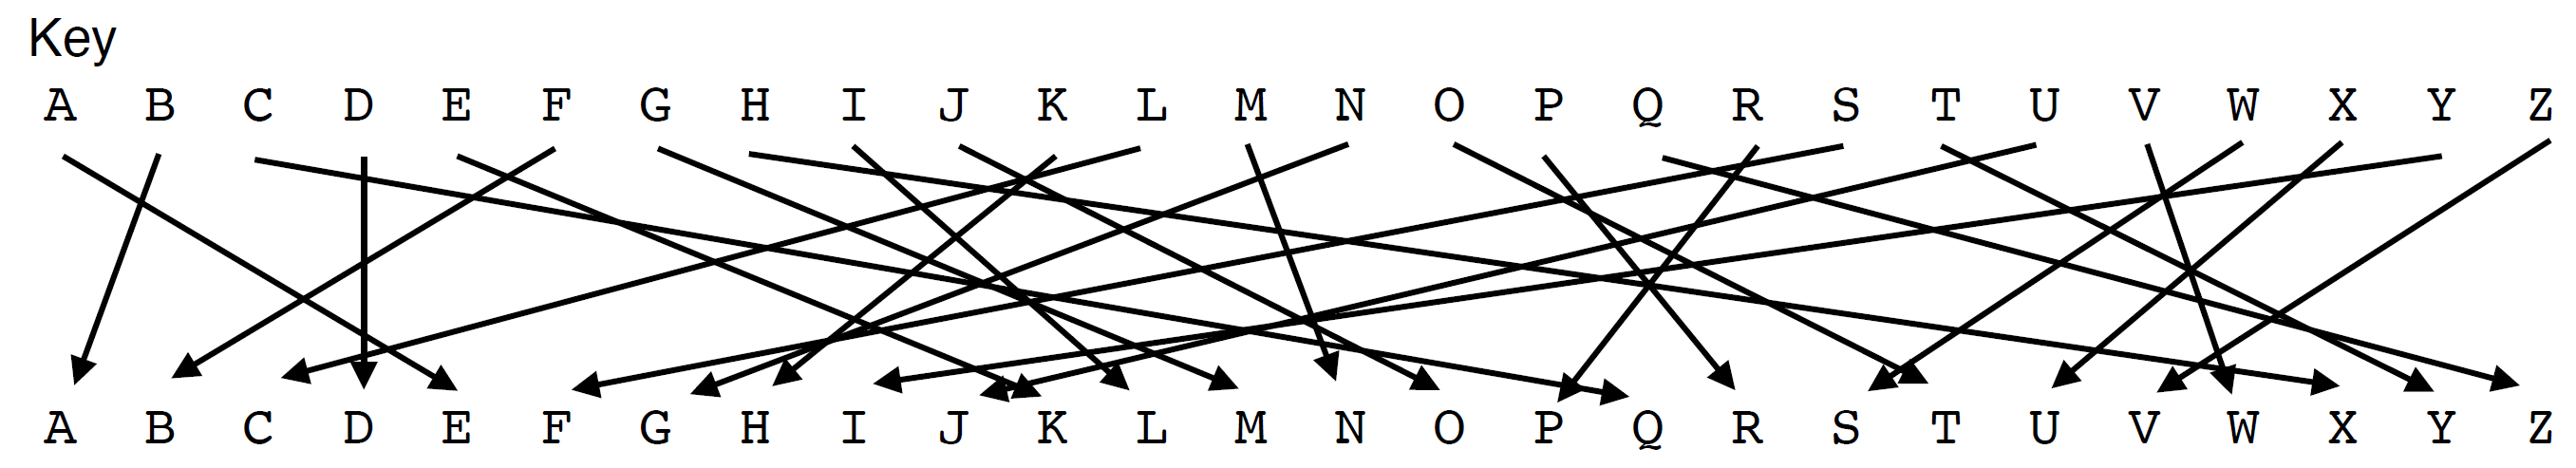
\includegraphics[width=160mm]{Graphics/Historical Ciphers/SubstitutionCiphers1.png}\newline
        \end{center}
        \begin{center}
            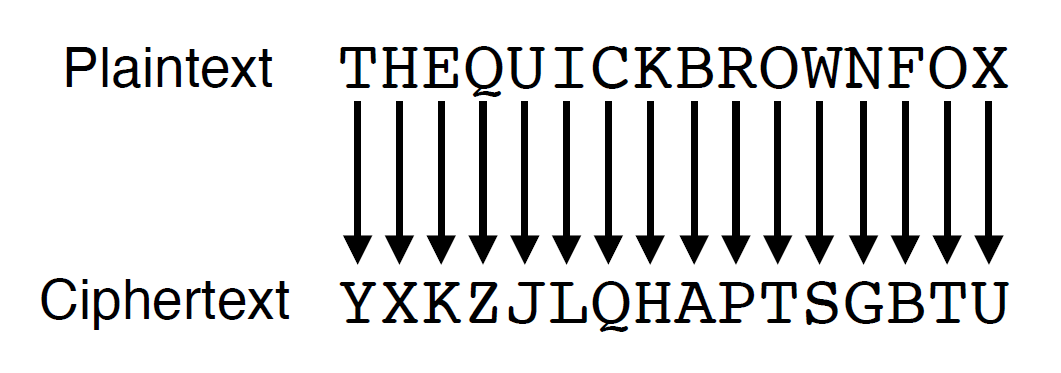
\includegraphics[width=80mm]{Graphics/Historical Ciphers/SubstitutionCiphers2.png}\newline
        \end{center}
        \begin{itemize}
            \item One of the oldest cipher in the world, used in the bible (Atbash)
            \item $\#Keys = 26! \gg 2^{86}$
        \end{itemize}
    
    \section{Caesar Cipher}
        \begin{itemize}
            \item Key is a fixed substitution table which shifts every letter by 3
            \item Encryption and decryption are as in the substitution cipher
        \end{itemize}
        \textbf{Shift Cipher}
        \begin{itemize}
            \item Generalization of Ceasar's Cipher: Variable Shift
            \item $\#Keys = 26$
        \end{itemize}
     
    \section{Vigènere Cipher}
    	\begin{itemize}
    		\item Variant of Caesar/Shift Cipher
    		\item Polyalphabetic Cipher: Not same shift for every plaintext character
    		\item $\# Keys = 26^n$
    	\end{itemize}
    	\begin{center}
          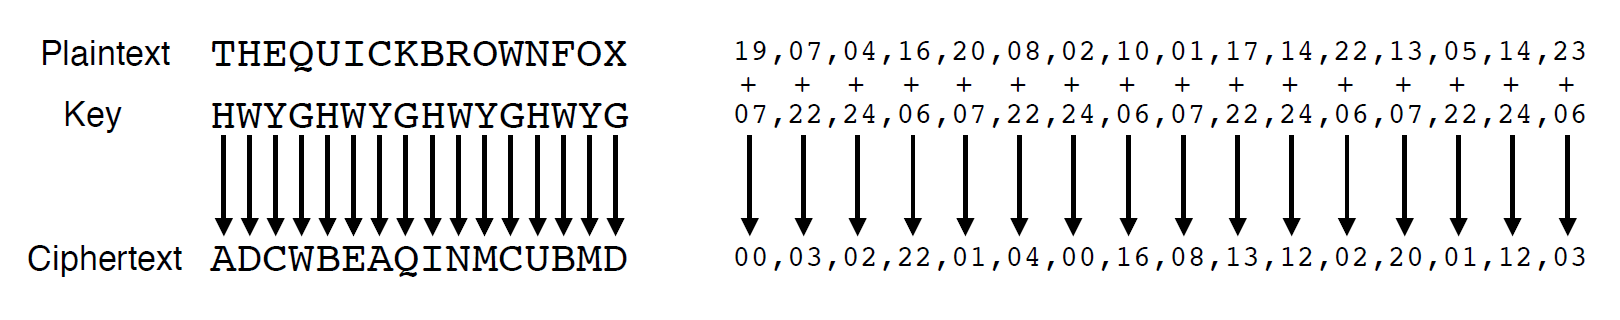
\includegraphics[width=140mm]{Graphics/Historical Ciphers/VigenereCipher.png}\newline
       \end{center}
	
	\section{Cryptanalysis}
		\begin{itemize}
			\item Scytale: Curvature of leather belt is give away
			\item Caesar Scheme: No key! Insecure once the method of encryption is known
			\item Shift Cipher: Key-space too small! Try all 26 keys
			\item What about the substitution and Vigènere ciphers?
		\end{itemize}
		
	\section{Frequency Analysis}
		\begin{itemize}
			\item Idea: Short piece of English text has similar statistics as English language as a whole
			\item Count letter frequencies in natural language
			\item Used for Vigènere Ciphers
		\end{itemize}
    	\begin{center}
         	 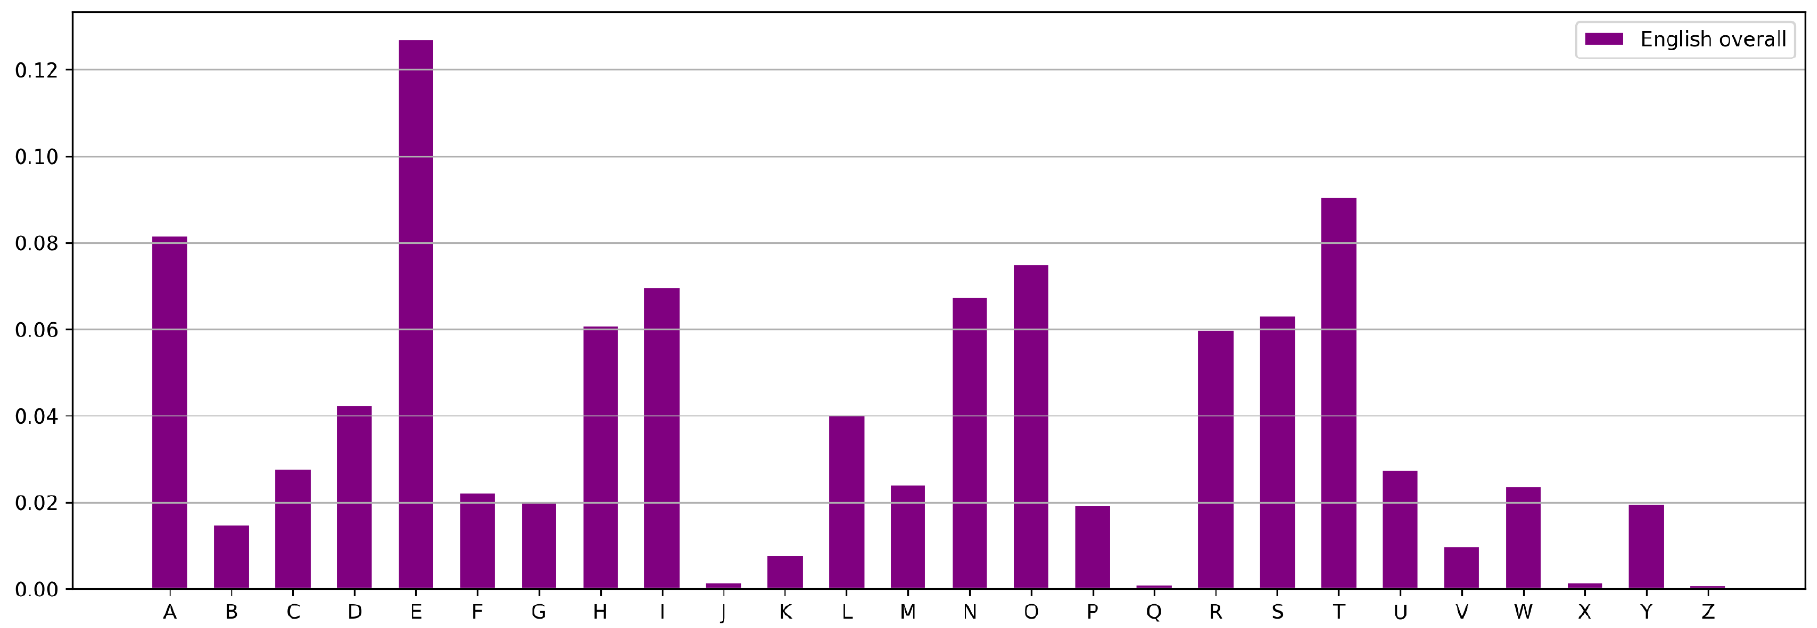
\includegraphics[width=180mm]{Graphics/Historical Ciphers/FrequencyAnalysis.png}\newline
       \end{center}
	
	\section{Cryptanalysis of the Substitution Cipher}
		\begin{itemize}
			\item Natural language also has frequent character constellations
			\item Generalize character frequencies: Bigrams, trigrams … N-grams
			\item Plaintext recovery requires a lot of context information and guessing
		\end{itemize}
		\begin{center}
         	 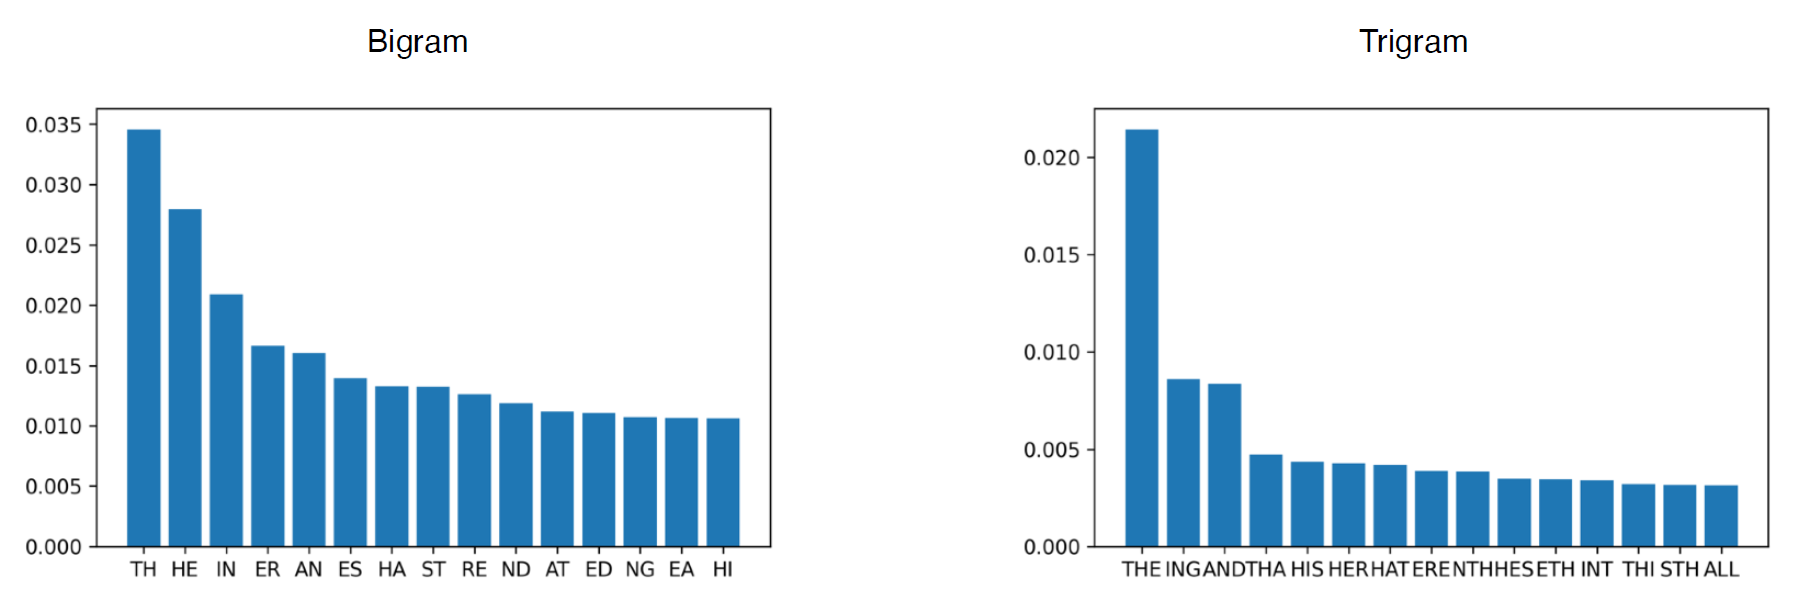
\includegraphics[width=160mm]{Graphics/Historical Ciphers/CryptanalysisSubstitutionCipher1.png}
       \end{center}
       \begin{itemize}
       	\item Plaintext recovery is strongest possible attack
       	\item Requires context information
       	\item More prior knowledge?
       	\item Maximum context information: Ciphertext encrypts one of two messages
       	\item Structural Property of Cipher: Same letters always encrypt to same letter
       \end{itemize}
       \begin{center}
         	 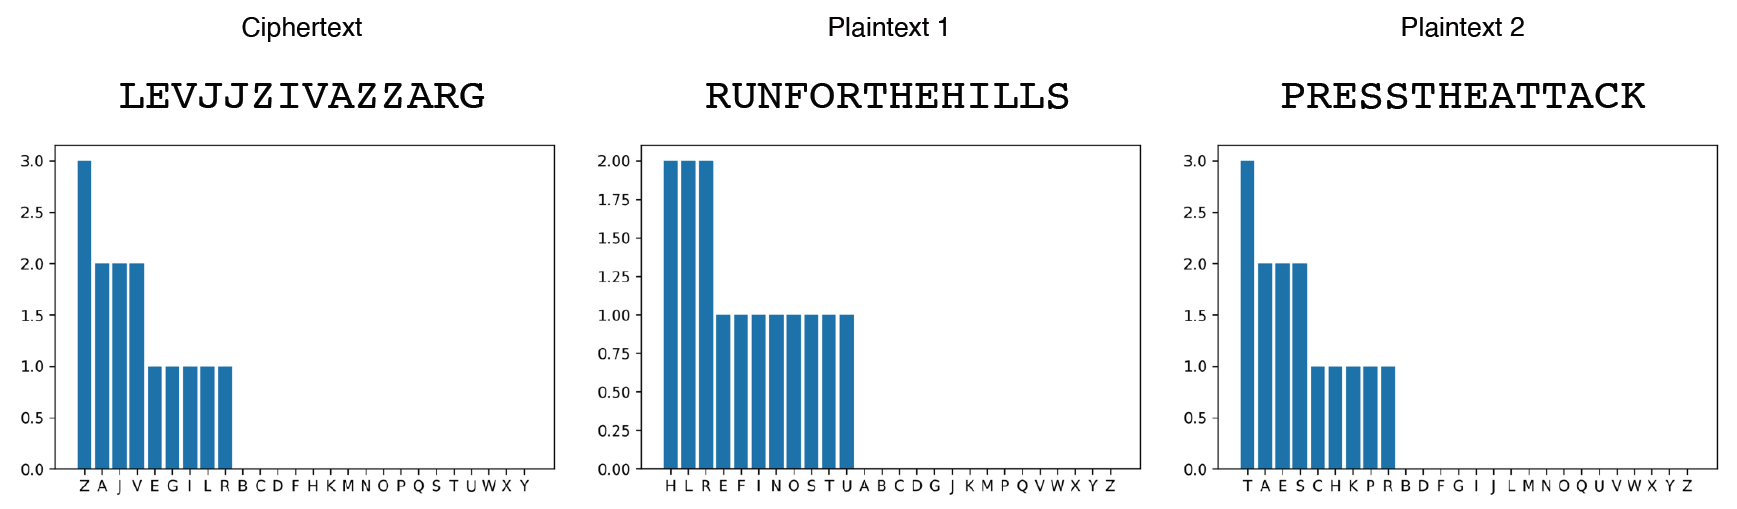
\includegraphics[width=160mm]{Graphics/Historical Ciphers/CryptanalysisSubstitutionCipher2.png}\newline
       \end{center}
    
    \section{Summary}
    	\begin{itemize}
    		\item Historical Ciphers were based on simple character substitution patterns
    		\item Typically small keys spaces
    		\item Can be broken with simple statistical analysis
    		\item Security relied mostly on the fact the method of encryption was not known to the adversary
    	\end{itemize}
    
    \section{Enigma}
    	\begin{itemize}
    		\item Enigma was a family of cipher machines used before and during WWII
    		\item Several of those were used by German forces during WWII
    		\item Cryptanalysis of these machines focused huge Allies effort
    		\item In particular, Turing and Blechtley park
    	\end{itemize}
    	
    	\subsection{General Architecture of Enigma}
    		\begin{itemize}
    			\item Rotor machine with input keyboard and output device
    			\item Includes several layers of transformations to perform encryption
    			\item Encryption is performed letter by letter
    			\item The transformations evolve with time to prevent direct frequency analysis
    			\item The cipher was an involution
    		\end{itemize}
    	
    	\subsection{Basic principle}
    		\begin{itemize}
    			\item Mix of mechanical and electrical technology
    			\item With the light output display : electric circuit from keyboard to lights
    			\item Goes through several stages into and out of the machine
    			\item Mechanical evolution after every key is released
    		\end{itemize}
    		\begin{center}
         	 	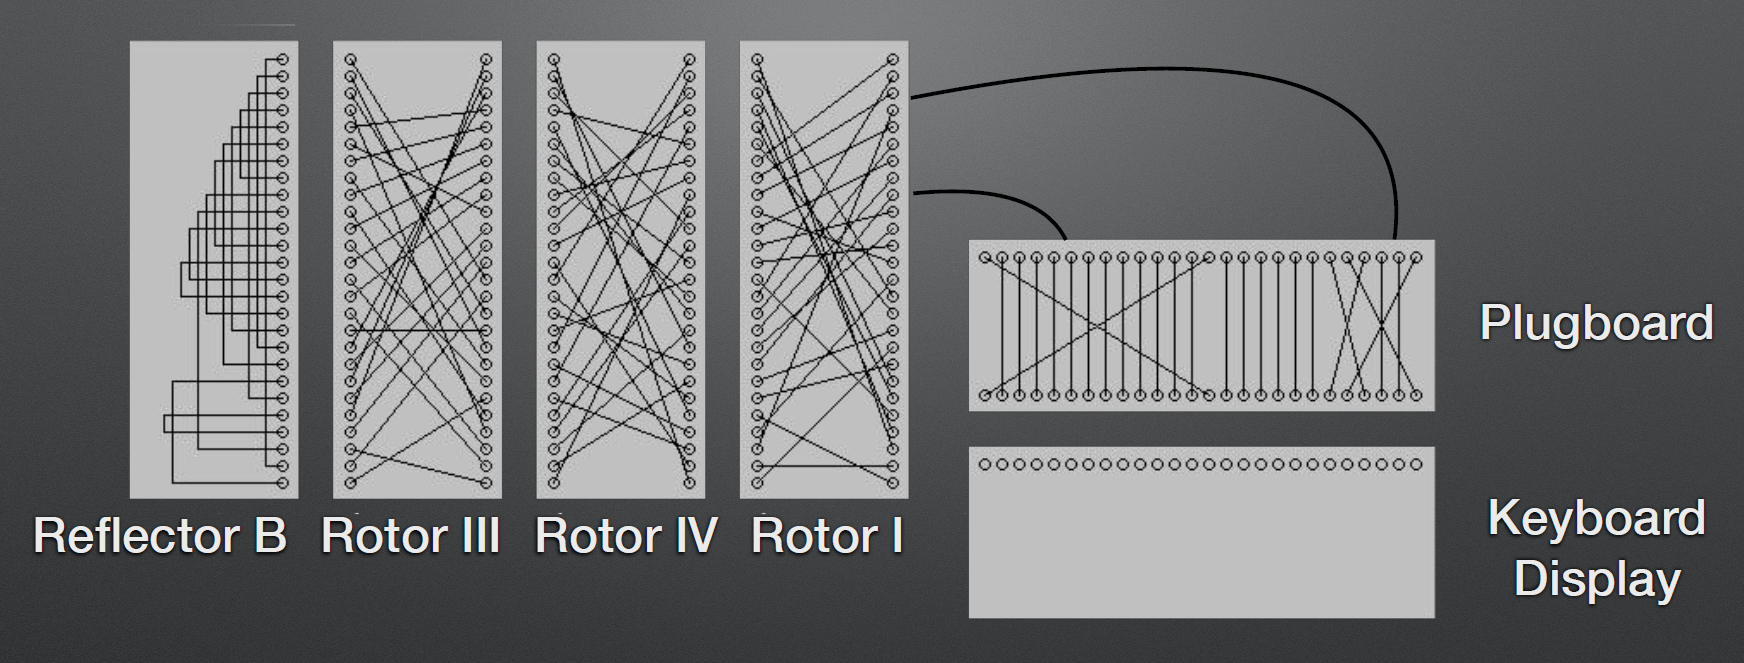
\includegraphics[width=180mm]{Graphics/Historical Ciphers/Enigma.png}\newline
       		\end{center}
       
       	\subsection{Key Size}
       		\begin{itemize}
       			\item Per message key:
       				\begin{itemize}
       					\item 17.576 possibilities (with 3 rotors) $\approx$ 14 bits
       					\item 456.976 possibilities (with 4 rotors) $\approx$ 19 bits
       				\end{itemize}
       			\item Daily key (4 rotor case)$\approx$ 78 bits:
       				\begin{itemize}
       					\item 2 choices of reflector
       					\item 2 choices of fourth rotor
       					\item 336 choices of first three rotors (in set of 8)
       					\item Ring setting : 456.976 possibilities
       					\item Arbitrary plugboard pairing (up to 13 plugs):
       					532.985.208.200.576 possibilities
       				\end{itemize}
       		\end{itemize}
       		Note: There is a dependency between daily and message key\\
       		Total key size $\approx$ 87.5 bits
       	
		\subsection{Digital rewriting of Enigma}
			\begin{itemize}
				\item View the encryption as a sequence of (evolving) permutations on letters
				\begin{itemize}
					\item Step 1: Swap letters according to plugboard
					\item Step 2, 3, 4, (5): Apply permutations corresponding to each rotor in order
					\item Mid Step: Apply (involutive) permutation of the reflector
					\item Step (-5), -4, -3, -2 : Apply inverse rotor permutations
					\item Step -1: Swap letters according to plugboard
				\end{itemize}
				\item Evolve Rotors state
			\end{itemize}

		\subsection{Reflector Permutations}
			\begin{center}
         		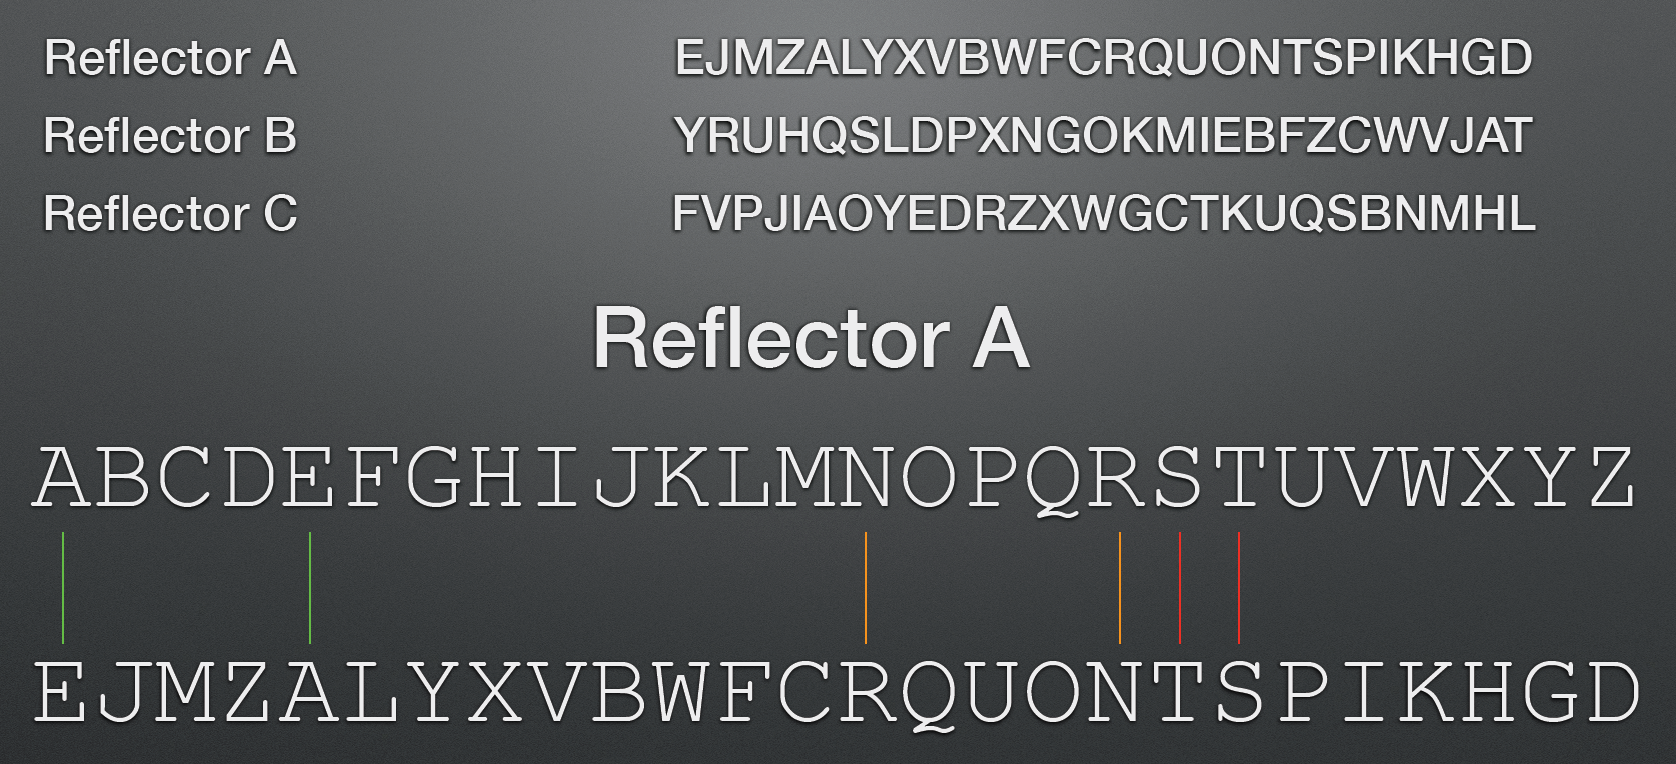
\includegraphics[width=180mm]{Graphics/Historical Ciphers/Enigma2.png}\newline
       		\end{center}
       	
       	\subsection{Rotor Permutations}
       		\begin{center}
         		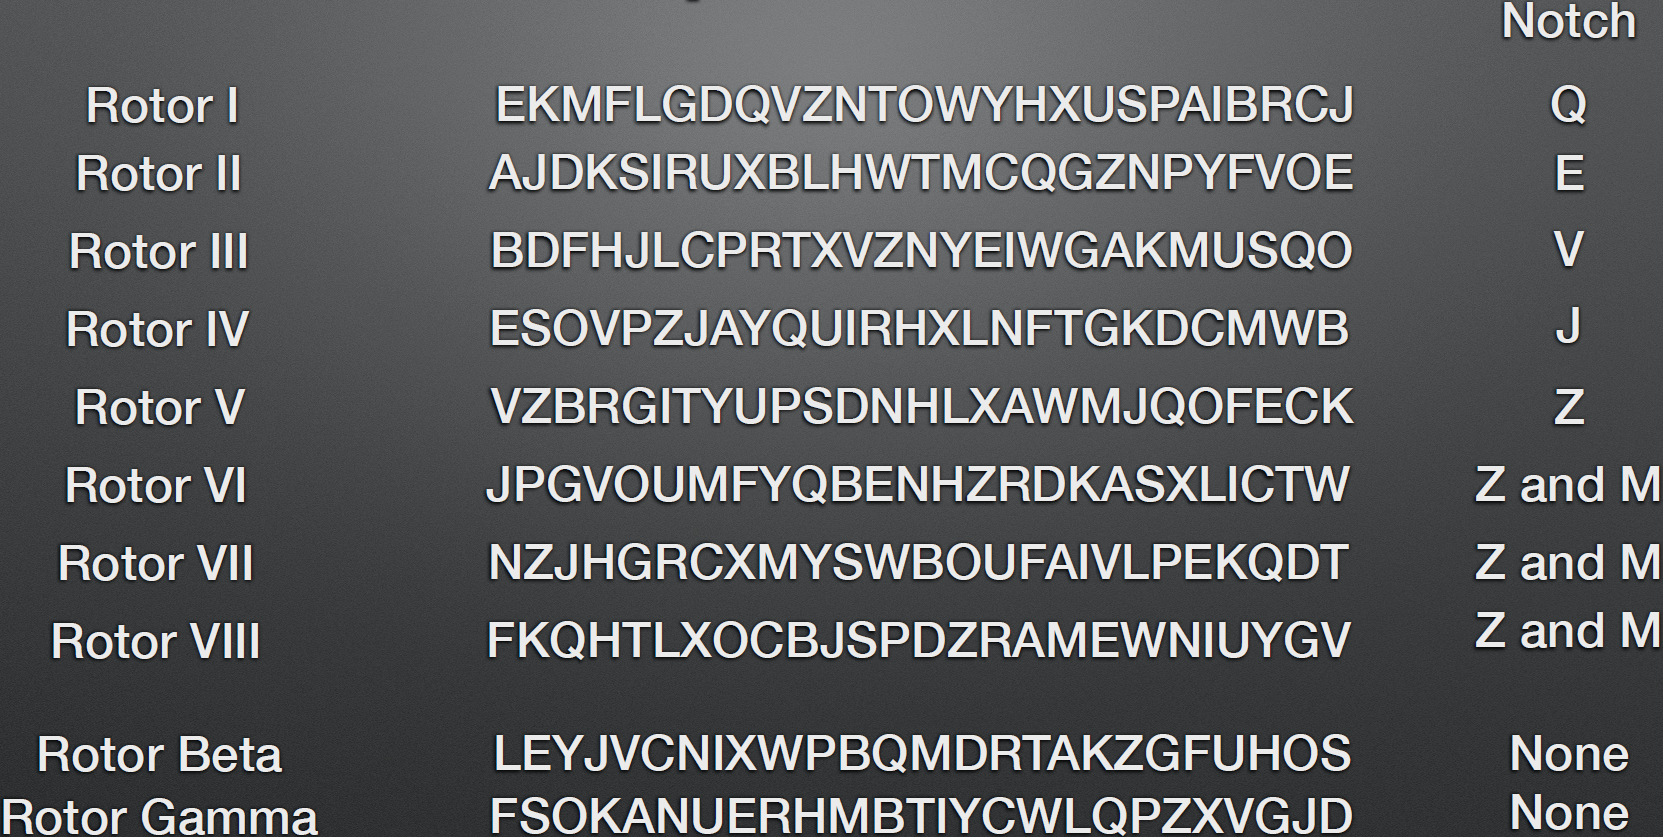
\includegraphics[width=180mm]{Graphics/Historical Ciphers/Enigma3.png}\newline
       		\end{center}
       		\begin{center}
         		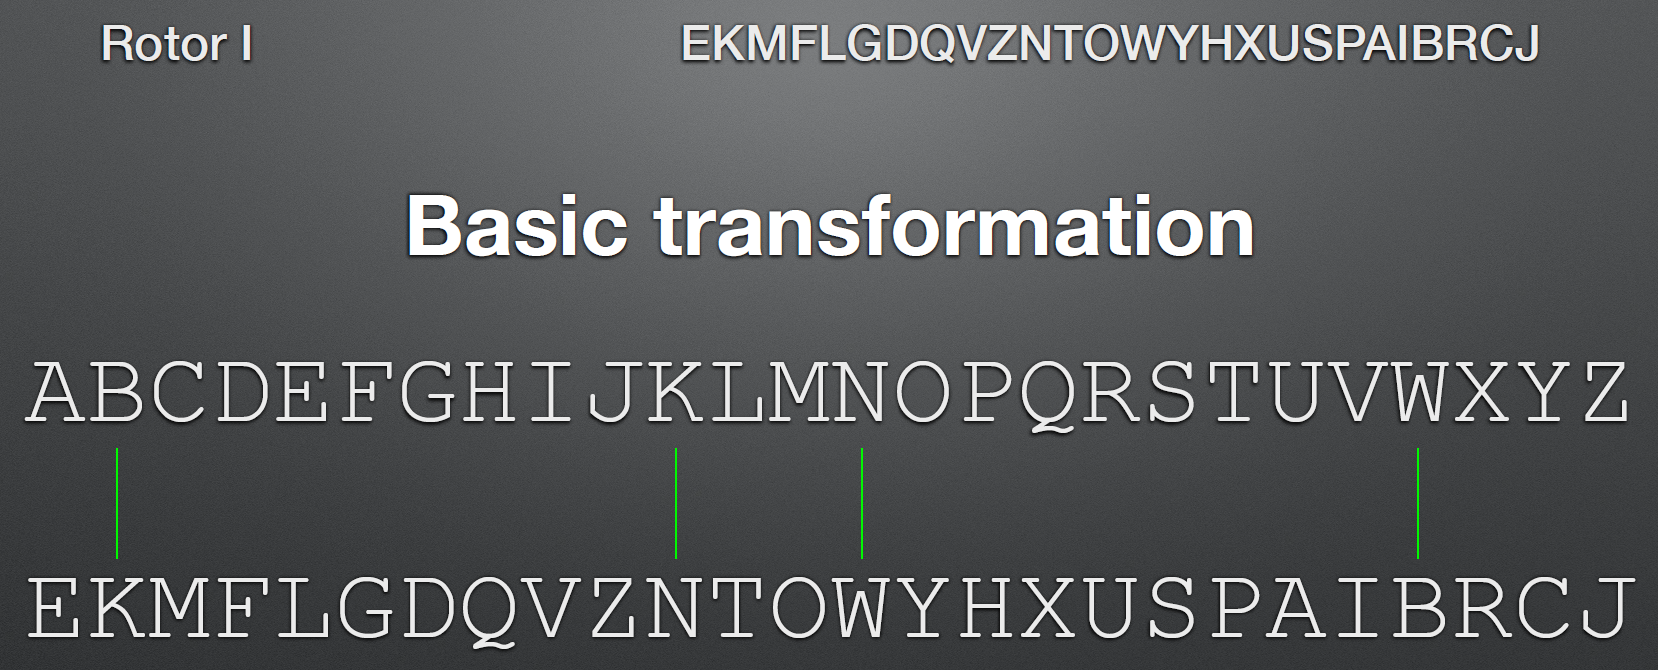
\includegraphics[width=180mm]{Graphics/Historical Ciphers/Enigma4.png}\newline
       		\end{center}
       	
       	\subsection{Rotor permutations (after rotation)}
       		\begin{center}
         		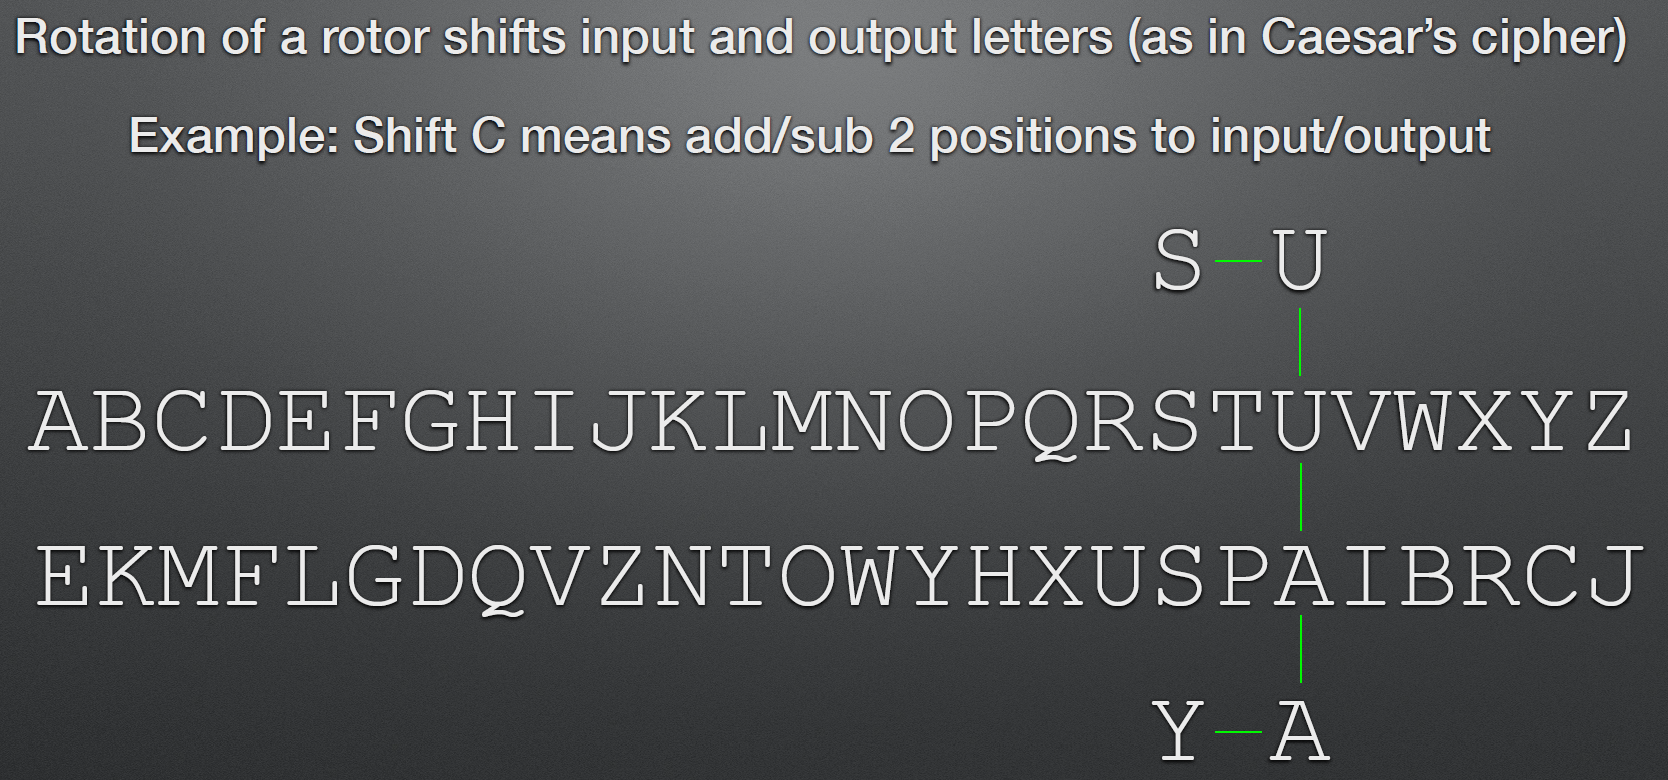
\includegraphics[width=180mm]{Graphics/Historical Ciphers/Enigma5.png}\newline
       		\end{center}
       	
       	\subsection{Plugboard}
       		\begin{center}
         		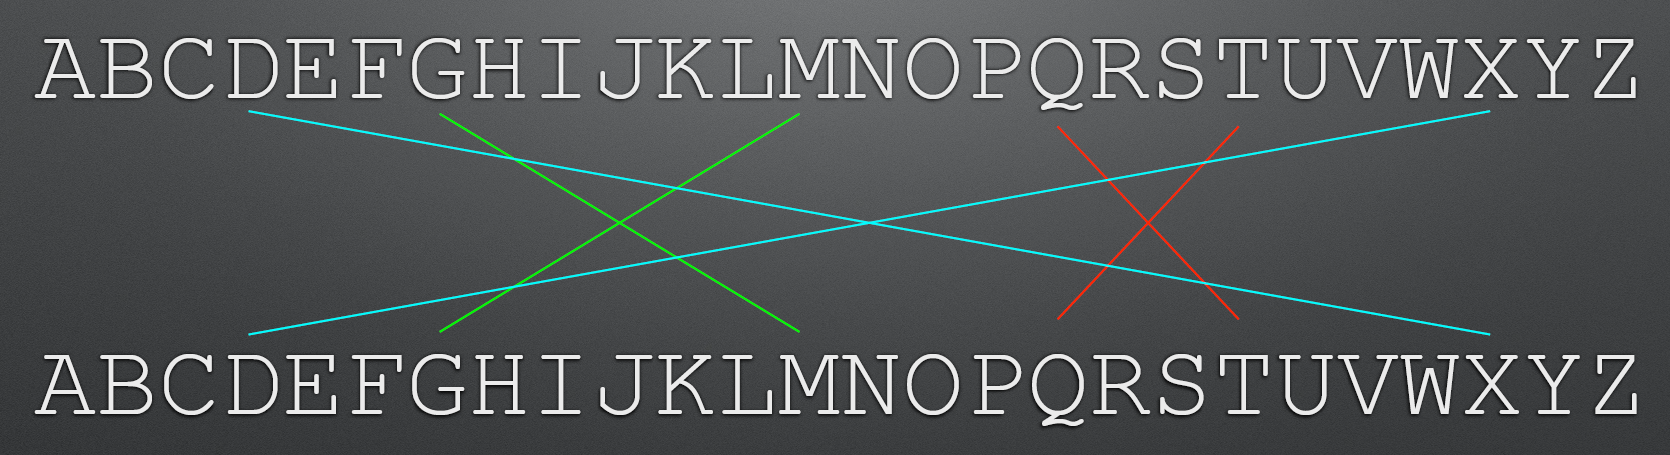
\includegraphics[width=180mm]{Graphics/Historical Ciphers/Enigma6.png}\newline
       		\end{center}
       	
       	\subsection{Rotor Evolution}
       		\begin{itemize}
       			\item Basic evolution: After every key release, rotate right rotor by 1 letter
       				\begin{itemize}
       					\item State A goes to B, B to C, … Y to Z and Z to A
       				\end{itemize}
       			\item Second rotor: If right rotor in notch pos. before change, rotate second rotor
       			\item Third rotor: If second rotor in notch pos., rotate third AND second rotors
       			\item Fourth rotor (optional): Never rotates
       		\end{itemize}
       	
       	\subsection{A simple property of Enigma}
       		\begin{itemize}
       			\item At every time t, the current transformation is an involution with no fixed point
       			\item Proof:
       				\begin{itemize}
       					\item By inspection, this is true for reflectors.
       					\item Let $\pi$ denote the reflector permutation and $\sigma$ be the current permutation of rotors/plugboard.
       					Then, the global permutation is $\sigma^{-1} \circ \pi \circ \sigma$.
       					\item It is an involution since
       					$(\sigma^{-1} \circ \pi \circ \sigma) \circ (\sigma^{-1} \circ \pi \circ \sigma) = \sigma^{-1} \circ \pi \circ \pi \circ \sigma = \sigma^{-1} \circ \sigma = Id$.
       					\item No fixed point since $\sigma^{-1} \circ \pi \circ \sigma(X) = X \implies \pi \circ \sigma(X) = \sigma(X)$\\
       					(impossible for $\pi$).
       				\end{itemize}
       		\end{itemize}
       	
       	\subsection{Modern view on Enigma}
       		\begin{itemize}
       			\item Trivially broken with modern standards
       			\item Example attack 1 (Chosen plaintext distinguisher):\\
       			Encrypt AAA….AAA (100 letters): 
       			Enigma encryption never contains A while random string of the same length has A with prob > 98%
       			\item Example attack 2 : The message is malleable letter by letter
       			\item Example attack 3 (Chosen plaintext attack): 
       			To decrypt challenge cipher text, simply feed it as plaintext to an encryption blackbox. 
       			Because of the involution property, get original plaintext back.
       			\item A simple key recovery faster than exhaustive search
       			\item Important : The cipher has a fixed part and a time varying part.\\
       			More precisely at time $t$ it can be written as $F^{-1} \circ V_t \circ F$.
       			\begin{itemize}
       				\item The fixed part comprised the plugboard and the initial position of first rotor.
       				\item The varying part is the rotors, reflectors and varies with rotations.
       			\end{itemize}
       			\item Key size for $F$ is 26 x 532.985.208.200.576 possibilities $\approx$ 53.6 bits.
       			\item Key size for $V_t$ is 2 x 2 x 336 x 265 possibilities $\approx$ 33.9 bits.
       		\end{itemize}
       	
       	\subsection{Recovering $V_t$ by "cheap" brute force}
       		\begin{itemize}
       			\item We can "fingerprint" $V_t$ with no information on $F$
       			\item Encrypt AAAAA...AAAAAA to $L_1L_2...L_n$ where $L_i = F^{-1} \circ V_i \circ F(A)$
       			\item Note that $L_i = L_j \Leftrightarrow V_i(X)=V_j(X)$ where $X = F(A)$
       			\item Enumerate $X$ and the key of the sequence $V_t$.
       			\item Cost $\approx$ 38.6 bits (with 4 rotos) - At first glance, $+ log_2(n)$ but avoidable
       		\end{itemize}
       	
       	\subsection{Practical Version}
       		\begin{itemize}
       			\item Data collection: Encrypt a sequence of 46 consecutive A — discard first 3
       			\item Fingerprint the 43 letters truncated encrypted sequence as follows:
       				\begin{itemize}
       					\item To each of the last 12 letters:
       						\begin{itemize}
       							\item Associate the position of the first letter in the first 31 that matches it
       							\item If no match, associate the value 0
       						\end{itemize}
       					\item This fingerprint has 60 bits and doesn’t depend on $F$ (except for $F(A)$)
       					\item Enough to identify the varying part $V$ (almost) uniquely
       					\item Once $V$ is obtained, recovering F fully is easy
       				\end{itemize}
       		\end{itemize}




































\chapter{Principles}

	\section{Lessons from Historic Ciphers}
		\begin{itemize}
			\item Ciphers without keys or small key-space cannot recover from compromise
			\item Ciphertext should not reveal statistical information about plaintexts
			\item Ciphertexts should not reveal any (efficiently computable) information about the plaintext
			\item Further thoughts: Many historic ciphers immediately broken given a single message-ciphertext pair
			\item Ciphers were designed with limited imagination
			\item \textbf{How do you defend against an adversary who is smarter than you?}
		\end{itemize}
	
	\section{Kerkhoff's Principle}
		\begin{center}
			\textbf{The cipher method must not be required to be secret, and it must be able to fall into the hands of the enemy without inconvenience.}
		\end{center}
		\begin{itemize}
			\item Designs which violate Kerkhoff's principle hope to achieve Security by Obscurity
			\item Today this is considered bad cryptographic design
			\item It is easier to switch a compromised key than a compromised design
		\end{itemize}
	
	\section{Principles of Modern Cryptography}
		\begin{itemize}
			\item \textbf{Formal Definitions/Models}
				\begin{itemize}
					\item What constitutes a successful attack?
					\item What is the goal of an attack?
				\end{itemize}
			\item \textbf{Precise Assumptions}
				\begin{itemize}
					\item Underlying hard problem?
				\end{itemize}
			\item \textbf{Formal Proofs}
				\begin{itemize}
					\item Show that a successful attack actually violates the assumptions
				\end{itemize}
		\end{itemize}
	
	\section{Formal Models}
		\begin{itemize}
			\item Example: Encryption
			\item We will generally define security by defining what it means that a scheme is insecure.
			\begin{itemize}
				\item What is the computational power of the adversary?
				\item What information is given to the adversary?
				\begin{itemize}
					\item Only Ciphertext
					\item A message and a ciphertext encrypting this message
					\item A ciphertext encrypting a message chosen by the adversary?
					\item Access to a “decryption oracle”
				\end{itemize}
				\item What is the goal of the adversary?
				\begin{itemize}
					\item Recover the key
					\item Recover the message
					\item Recover parts of the message
					\item Distinguish encryptions of two messages
				\end{itemize}
			\end{itemize}
		\end{itemize}
	
	\section{Precise Assumptions}
		\begin{itemize}
			\item Should it be impossible to break the cipher only hard?
			\item How can we mathematically define hard problems?
			\begin{itemize}
				\item Complexity Theory!
				\item Example: Factor large numbers
			\end{itemize}
			\item A good assumption should be simple to state but hard to break
		\end{itemize}
		\textbf{Precise Assumptions let us}
		\begin{itemize}
			\item Falsify an assumption by cryptanalysis
			\item Build confidence by lack of cryptanalysis
			\item Compare schemes by their underlying assumptions
			\item Understand the necessity of the assumption
		\end{itemize}
	
	\section{Summary}
		\begin{itemize}
			\item Kerkhoff’s principle: Only the key should be secret, not the scheme itself
			\item Modern cryptography evolved into a discipline following scientific principles
			\item It lets us design schemes secure against adversaries smarter than ourselves!
		\end{itemize}




















\chapter{Probability Theory}

	\section{Why Randomness and Probability?}
		\textbf{Probability Theory:}
		Mathematical framework for systems which behave in unpredictable or random ways
		
		\begin{itemize}
			\item \textbf{Most Sciences:} Systems too complex for exact modeling, lack of precise measurements
			\item \textbf{Computer Science:} Randomness is a resource
			\item \textbf{Cryptography:} Impossible without randomness!
		\end{itemize}
	
	\section{How can randomization lead to efficient algorithms?}
		\begin{itemize}
			\item Example: Election Winners
			\item You have an election with 40 million voters and want to know quickly who is the (likely) winner
			\item You want to know who the winner is without counting all votes
			\item Idea: Take a \textbf{random sample} of 1000 votes determine the winner!
		\end{itemize}
	
	\section{Probability Spaces}
		A finite probability space consists of two components:
		\begin{enumerate}
			\item A finite set $\Omega$ called the sample space.
			\item A probability function $Pr: \Omega \to \mathbb{R}$ satisfying
				\begin{itemize}
					\item For all $\omega \in \Omega$: $0 \leq Pr[\omega] \leq 1$
					\item $\sum\limits_{\omega \in \Omega} Pr[\omega] = 1$
				\end{itemize}
		\end{enumerate}
		\begin{itemize}
			\item The $\omega\in \Omega$ are called elementary events or outcomes
			\item A set $E \subseteq \Omega$ is called event
			\item For an event $E$ define
				\begin{center}
					$Pr[E] = \sum\limits_{\omega \in E} Pr[\omega]$
				\end{center}
				where $Pr[\emptyset] = 0$
		\end{itemize}
	
	\section{Set Operations on events}
		\begin{itemize}
			\item The intersection $E_1 \cap E_2$ of two events $E_1$ and $E_2$ is interpreted as the logical "and" of two events.
			Depending on the context, we will use the following notations
			\begin{center}
				$Pr[E_1 \cap E_2] =: Pr[E_1,E_2] =: Pr[E_1 \wedge E_2] =: Pr[E_1 \  and \  E_2]$
			\end{center}
			\item The union $E_1 \cup E_2$ of two events $E_1$ and $E_2$ is interpreted as the logical "or" of two events.
			Thus, we will use the following notation
			\begin{center}
				$Pr[E_1 \cup E_2] =: Pr[E_1 \vee E_2] =: Pr[E_1 \  or \  E_2]$
			\end{center}
			\item The complement $\bar{E} = \Omega \backslash E$ of an event $E$ is interpreted as the logical "negation" of $E$.
			We will use the notation
			\begin{center}
				$Pr[\bar{E}] =: Pr[\neg E] =: Pr[not \  E]$
			\end{center}
			\item If $A \subseteq B$ we say that the event $A$ implies the event $B$ and also write $A \Rightarrow B$
		\end{itemize}
	
	\section{Properties of Probability Spaces}
		\begin{itemize}
			\item For all events $A,B \subseteq \Omega$:
				\begin{enumerate}
					\item $Pr[A \cup B] = Pr[A] + Pr[B] - Pr[A \cap B]$
					\item $Pr[\bar{A}] = 1 - Pr[A]$
					\item If $A \subseteq B$ then $Pr[A] \leq Pr[B]$
				\end{enumerate}
			\item Item 1 implies the \textbf{union-bound}:\\
			For all $A,B \subseteq \Omega$ it holds $Pr[A \cup B] \leq Pr[A] + Pr[B]$
		\end{itemize}
	
	\section{Conditional Probabilities and Independence}
		\begin{itemize}
			\item For two events $A$ and $B$ we define the conditional probability 
			\begin{center}
				$Pr[A|B] = \frac{Pr[A \cap B]}{Pr[B]}$, $Pr[B] > 0$
			\end{center}
			\item Two events $A,B \subseteq \Omega$ are called independent if
			\begin{center}
				$Pr[A \cap B] = Pr[A] \cdot Pr[B]$
			\end{center}
			\item This is equivalent to $Pr[A|B] = Pr[A]$
			\item By symmetry also to $Pr[B|A] = Pr[B]$
		\end{itemize}

	\section{Bayes' Rule}
		\begin{itemize}
			\item Bayes’ rule relates the conditional probabilities $Pr[A|B]$ and $Pr[B|A]$
			\item This is especially useful when analyzing larger processes composed of smaller ones
		\end{itemize}
		\textbf{Bayes' Rule}\newline
		For all $A,B \subseteq \Omega$, it holds for $Pr[A],Pr[B] > 0$, that
		\begin{center}
			$Pr[A|B] = \frac{Pr[B|A] \cdot Pr[A]}{Pr[B]}$
		\end{center}
		
		\begin{proof}
		$Pr[A|B] = \frac{Pr[A \cap B]}{Pr[B]} \cdot \frac{Pr[A]}{Pr[A]} = \frac{Pr[A \cap B]}{Pr[A]} \cdot \frac{Pr[A]}{Pr[B]} 
		= \frac{Pr[B \cap A]}{Pr[A]} \cdot \frac{Pr[A]}{Pr[B]} = \frac{Pr[B|A] \cdot Pr[A]}{Pr[B]}$
		\end{proof}
		
	\section{Law of Total Probability}
		\begin{itemize}
			\item Sometimes we want to infer the probability of an event given conditional probabilities of this event
			\item This will also be useful to compute/bound probabilities by a case analysis
		\end{itemize}
		\textbf{Law of Total Probability}\newline
		Let $B_1,...,B_n$ be events that partition the probability space $\Omega$, i.e. $B_1 \cup ... \cup B_n = \Omega$ and $B_i \cap B_j = \emptyset$ for $i \neq j$.
		Then it holds for every event $A$ that
		\begin{center}
			$\sum\limits_{i=1}^{n} Pr[A \cap B_i] = Pr[A]$, with $Pr[A \cap B_i] = Pr[A|B_i] \cdot Pr[B_i]$
		\end{center}
		
		\begin{proof}\ Preconditions:
			\begin{enumerate}
				\item $Pr[E_1 \cup E_2] Pr[E_1] + Pr[E_2]$ if $E_1 \cap E_2 = \emptyset$, and
				\item $Pr[E_1 \cup ... \cup E_n] = \sum\limits_{i=1}^{n} Pr[E_i]$ if $E_i \cap E_j = \emptyset$ for $i \neq j$.
				\item $Pr[A \cap B_i] = Pr[A|B_i] \cdot Pr[B_i]$
			\end{enumerate}
			We know that $A = A \cap \Omega = A \cap \Big( \bigcup\limits_{i=1}^{n} B_i \Big) = \bigcup\limits_{i=1}^{n} A \cap B_i$.\\
			So it follows $Pr[A] = Pr\Big[\bigcup\limits_{i=1}^{n} A \cap B_i\Big] \overset{\text{(2.)}}{=} \sum\limits_{i=1}^{n} Pr[A \cap B_i] 
			\overset{\text{(3.)}}{=} \sum\limits_{i=1}^{n} Pr[A | B_i]\cdot Pr[B_i]$.
		\end{proof}
		
	\section{Example: Bayes and LotP in Action}
		\begin{itemize}
			\item Assume 2 in 1000 people in a population have a certain disease
			\item There exists a test for this disease but it is not flawless
			\item If you have the disease, then there is a 95$\%$ chance that the test returns positive
			\item Moreover, there is a 3$\%$ chance that the test returns positive even if you don t have the disease
			\item Imagine, you do a test and it returns positive, what is the probability that you actually have the disease?
		\end{itemize}
		\textbf{Remarks:}
		\begin{itemize}
			\item The probability 2 1000 = 0.002 is your prior of having the disease, i.e. if you do not get the additional information of test, this is your best guess
			\item We are interested in the posterior probability
		\end{itemize}
		\textbf{Solution:}
		\begin{itemize}
			\item Let s model this with a probability space
			\item Let $A$ be the event that you have the disease. We know that $Pr[A] = 0.002$
			\item Let $B$ be the event that the test returns positive. We know that $Pr[B|A] = 0.95$
			\item We also know that $Pr[B|\bar{A}] = 0.03$
			\item We want to know the posterior $Pr[A|B]$
		\end{itemize}
		$Pr[A|B] = \frac{Pr[B|A] \cdot Pr[A]}{Pr[B]} = \frac{Pr[B|A] \cdot Pr[A]}{Pr[B|A] \cdot Pr[A] + Pr[B|\bar{A}] \cdot Pr[\bar{A}]} 
		= \frac{Pr[B|A] \cdot Pr[A]}{Pr[B|A] \cdot Pr[A] + Pr[B|\bar{A}] \cdot (1-Pr[A])} \approx 0.06$\\
		
		If you do a test and it returns positive, the probability that you actually have the disease is $6\%$!
		
	\section{Summary 1}
		\begin{itemize}
			\item Probability spaces model randomized processes
			\item Conditional probabilities tell us a posteriori probabilities given that some event has happened
			\item Bayes’ rule and the law of total probability simplify working with conditional probabilities
		\end{itemize}

\newpage

	\section{Random Variables}
		\begin{itemize}
			\item In general, any function $X: \Omega \to D$ for some domain $D$ is called a ($D$-valued) \textbf{random variable}
			\item We can now define events with respect to a random variable.
			\item Let $x \in D$ define the event $E_x = \{ \omega \in \Omega: X(\omega)=x \} \subseteq \Omega$
			\item We write the shorthand $X=x$ for $E_x$
			\item We call the function $F(x) = Pr[E_x] = Pr[X=x]$ the probability distribution of $X$
		\end{itemize}
	
		\subsection{Independence of random variables}
			\begin{itemize}
				\item Consider two random variables $X \in D_X$ and $Y \in D_Y$, which means $X: \Omega \to D_X$ and $Y: \Omega \to D_Y$
				\item We say that $X$ and $Y$ are \textbf{independent}, if it holds for all $x \in D_X$ and $y \in D_Y$ that the events $X=x$ and $Y=y$ are independent
				\item I.e. $Pr[X=x,Y=y] = Pr[X=x] \cdot Pr[Y=y]$
			\end{itemize}
		
		\subsection{Examples}
			\begin{itemize}
				\item \textbf{Identity function:}\\
					$X: \Omega \to \Omega$. In this case $Pr[X=\omega] = Pr[\omega]$.
				\item \textbf{Projections:}\\
					Let $\Omega \subseteq D_1 \times D_2$, then $X: \Omega \to D_1$, $(x,y) \mapsto x$ and $Y: \Omega \to D_2$, $(x,y) \mapsto y$ are projections.
				\item \textbf{Reverse direction:}\\
					Given two sample spaces $\Omega_1$ and $\Omega_2$, we can form a new sample space $\Omega = \Omega_1 \times \Omega_2$.\\
					Then the projections $X: \Omega \to \Omega_1$ and $Y: \Omega \to \Omega_2$ are independent random variables.
				\item We say that a random variable $X: \Omega \to D$ is \textbf{uniform} on $D$ or an \textbf{uniform distribution}, if for every $x \in D$ 
					it holds $Pr[X=x] = \frac{1}{|D|}$
				\item \textbf{Sum of two dice rolls:}\\
					Let $\Omega = \{1,...,6\} \times \{1,...,6\}$, then $S: \Omega \to \mathbb{Z}$ with $(x,y) \mapsto x+y$ is a sum of two dice rolls.
				\item \textbf{Indicator random variable:}\\
				For an event $E$ we can define the random $X_E: \Omega \to \{0,1\}$ such that $X_E(\omega)=1$ if $\omega \in E$ and $X_E(\omega)=0$ if $\omega\notin E$
			\end{itemize}
		
		\subsection{Defining Probability Spaces via Random Variables}
			\begin{itemize}
				\item From now on we will omit the function notation for random variables
				\item Moreover, from now on we will also omit defining the sample space $\Omega$ explicitly
				\item Instead, we implicitly define $\Omega$ via a set of random variables
				\item General idea: The probability space is defined via a few independent "base" random variables
				\item All other random variables of interest depend on these deterministically
				\item When constructing a system that uses randomization, we do not need to keep track of the sample space, it is define "on the fly" as we introduce new random
				variables
				\item If $X$ is chosen uniformly random from some domain $D$, we will use the notation $X \leftarrow_{\$} D$ instead of the function notation
			\end{itemize}
		
		\subsection{Examples}
			\begin{itemize}
				\item Let $X_1,...,X_n$ be independent random variables such that each $X_i$ is uniform on $\{ 0,1 \}$.
				We say $X_1,...,X_n$ are \textbf{iid uniform on} $\{0,1\}$ for short
				\item Then $X = (X_1,...,X_n)$ is uniform on $\{0,1\}^n$
				\item $Y = X_1 + ... + X_n$ follow a distribution which is called the Bernoulli distribution
			\end{itemize}
			\begin{center}
				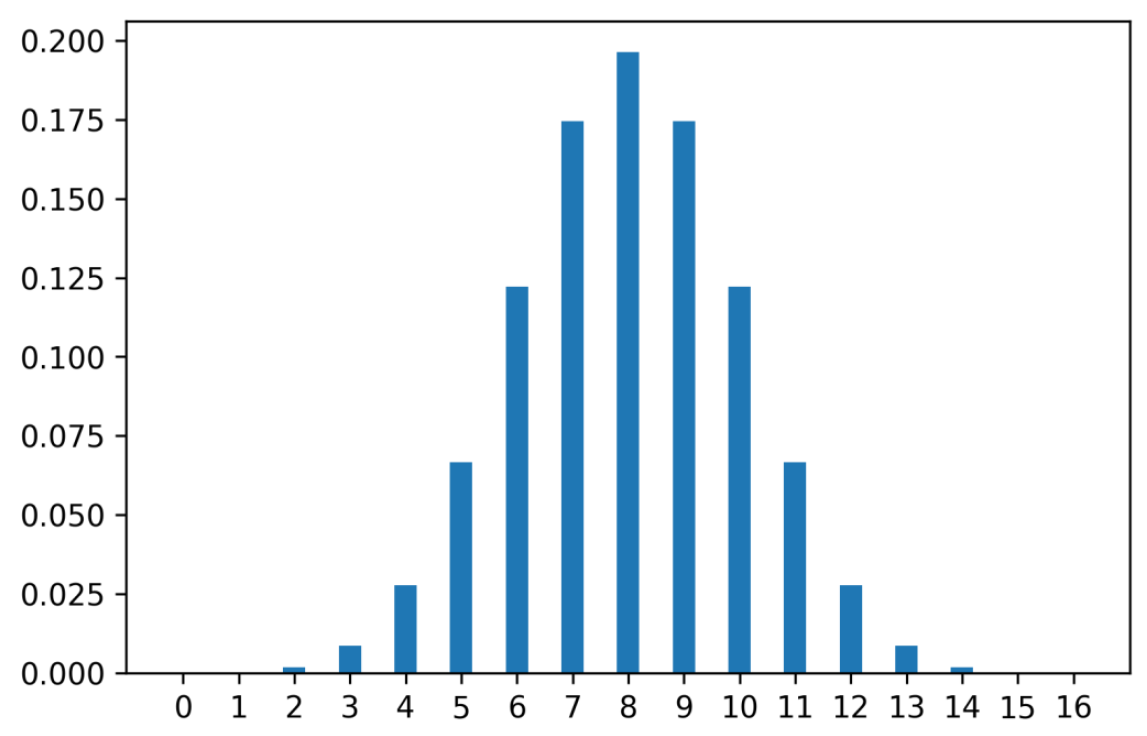
\includegraphics[width=120mm]{Graphics/Probability Theory/Examples1.png}\newline
			\end{center}
		
		\subsection{Sampling Algorithms}
			\begin{itemize}
				\item In general: We say a random variable $Z$ is \textbf{sampleable}, if there exists an (efficient) algorithm $M$ such that
				$Z = M(X_1,...,X_n)$, where $X_1,...,X_n$ are iid uniform on $\{0,1\}$
				\item $X_1,...,X_n$ are called the \textbf{random coins} or just \textbf{coins} of $M$
			\end{itemize}
			\begin{center}
            	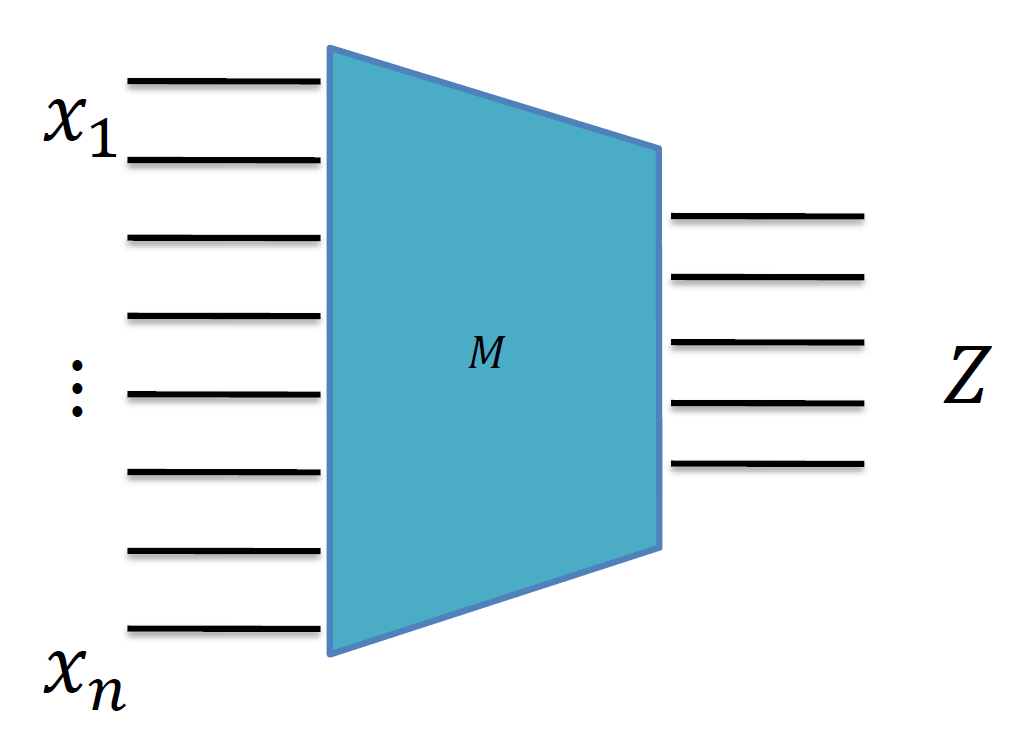
\includegraphics[width=120mm]{Graphics/Probability Theory/SamplingAlgorithms.png}\newline
        	\end{center}
        
	\section{Real-Valued Random Variables and Expectations}
		\begin{itemize}
			\item We call random variables $X: \Omega \to \mathbb{R}$ \textbf{real-valued}
			\item We call $Supp(X) = X(\Omega) \subseteq \mathbb{R}$ the \textbf{support} of $X$
			\item Note that $Supp(X)$ is finite as $\Omega$ is finite
			\item For a real-valued random variable $X$, we can define an \textbf{expectation}
				\begin{center}
					$E[X] = \sum\limits_{x \in Supp(X)} x \cdot Pr[X=x]$
				\end{center}
		\end{itemize}
		
		\subsection{Linearity of Expectation}
			\begin{itemize}
				\item Expectations are characteristic of random variables
				\item Powerful tool to analyze random variables constructed from other random variables
			\end{itemize}
			\textbf{Linearity of Expectation}\\
			Let $X$ and $Y$ be two real-valued random variables and $\alpha \in \mathbb{R}$ be a constant.\\
			Then it holds that
			\begin{enumerate}
				\item $E[\alpha \cdot X] = \alpha \cdot E[X]$
				\item $E[X+Y] = E[X]+E[Y]$
			\end{enumerate}
			Note: $X$ and $Y$ don't need to be independent
			
			\begin{proof}
			Proof of the linearity properties of expectation
			\begin{enumerate}
				\item To show: $E[\alpha \cdot X] = \alpha \cdot E[X]$
					\begin{align*}
						E[\alpha \cdot X] &= \sum\limits_{z \in Supp(\alpha \cdot X)} z \cdot Pr[\alpha \cdot X = z] \text{, with } \alpha \neq 0
					\end{align*}
					Now we make the following substitution: $z = \alpha \cdot z'$
					\begin{align*}
						E[\alpha \cdot X] &= \sum\limits_{z'} \alpha \cdot z' \cdot Pr[\alpha \cdot X = \alpha \cdot z']\\
						&= \alpha \cdot \sum\limits_{z'} \cdot Pr[X=z']\\
						&= \alpha \cdot E[X]
					\end{align*}
				
				\item To show: $E[X+Y] = E[X]+E[Y]$
					\begin{align*}
						E[X] &= \sum\limits_{x \in Supp(x)} x \cdot Pr[X=x]\\
						&= \sum\limits_{x \in S} x \cdot Pr[X=x] \text{, with } Supp(X),Supp(Y),Supp(X+Y) \leq S
					\end{align*}
					\begin{align*}			
						E[X+Y] &= \sum\limits_{z \in Supp(X+Y)} z \cdot Pr[X+Y = z]\\
						&= \sum\limits_{y \in Supp(Y)} \sum\limits_{z \in Supp(X+Y)} z \cdot Pr[X=z-y \wedge Y=y]\\
						&= \sum\limits_{y \in S} \sum\limits_{x \in S} (x+y) \cdot Pr[X=x, Y=y] \text{, with } z=x+y\\
						&= \sum\limits_{y \in S} \sum\limits_{x \in S} x \cdot Pr[X=x, Y=y] + \sum\limits_{y \in S} \sum\limits_{x \in S} y \cdot Pr[X=x, Y=y]\\
						&= \sum\limits_{x \in S} x \cdot \sum\limits_{y \in S} Pr[X=x, Y=y] + \sum\limits_{y \in S} y \cdot \sum\limits_{x \in S} Pr[X=x, Y=y]\\
						&= \sum\limits_{x \in S} x \cdot Pr[X=x] + \sum\limits_{y \in S} y \cdot Pr[Y=y]\\
						&= E[X] + E[Y]
					\end{align*}
			\end{enumerate}
			\end{proof}
		
		\subsection{Example}
			\begin{itemize}
				\item Let $X_1,...,X_n$ be independently distributed random variables on $\{0,1\}$ such that for all $i$ it holds $Pr[X_i=1] = p$ for a constant $p \in [0,1]$
				\item What is the expectation of $Y = X_1+...+X_n$?\\
					$E[Y] = E[X_1+...+X_n] = E[X_1] +...+ E[X_n] = n \cdot p$\\
					$Pr[X_i = 1] = p \Rightarrow E[X_i] = \sum\limits_{b \in \{0,1\}} b \cdot Pr[X_i = b] = Pr[X_i = 1] = p$
			\end{itemize}

	\section{A little detour to Algebra: Finite Groups}
		\subsection{Groups}
			A set $G$ together with a binary operation $\circ: G \times G \to G$ is called a group, if the following conditions are met:
			\begin{enumerate}
				\item \textbf{Associativity:} 
				For all $f,g,h \in G$ it holds that $(f \circ g) \circ h = f \circ (g \circ h)$
				\item \textbf{Identity Element:} 
				There exists a special element $e \in G$ such that for all $g \in G$ it holds $e \circ g = g \circ e = g$
				\item \textbf{Inverses Element:}
				For every $g \in G$ there exists an element $g^{-1} \in G$ such that $g \circ g^{-1} = e$
			\end{enumerate}
			\begin{itemize}
				\item A group $(G,\circ)$ is called \textbf{commutative (abelian) group} if for all $g,h \in G$ it holds $g \circ h = h \circ g$
				\item We say a group $(G,\circ)$ is \textbf{finite} if $G$ is finite as a set
			\end{itemize}
		
		\subsection{Examples of Groups}
			\begin{itemize}
				\item The integers under addition: $(\mathbb{Z},+)$
				\item Modular integers under addition: $(\mathbb{Z}/n\mathbb{Z}, +\ mod\ n)$
				\item The non-zero rational numbers under multiplication: $(\mathbb{Q} \backslash \{0\}, \cdot)$
				\item The binary set under XOR: $(\{0,1\}, \oplus)$
				\item Binary vectors under XOR: $(\{0,1\}^n, \oplus)$ with $\oplus$ bitwise
			\end{itemize}
		
		\subsection{Random Variables in Groups}
			\begin{itemize}
				\item Let $U$ be uniformly distributed on a \textbf{finite group} $G$
				\item I.e. for all $g \in G$ it holds $Pr[U=g] = \frac{1}{|G|}$
				\item Fix an $z \in G$, what is the probability distribution of $U \circ z$?
				\item $\Rightarrow$ If $U$ is uniformly distributed on $G$ and $Z$ is a random variable supported on $G$ and independent of $U$, 
				then $U \circ Z$ is also uniformly distributed on $G$
				\item In particular for $G = \{0,1\}$ and $\circ = \oplus$, $U \oplus Z$ is distributed uniformly random.
			\end{itemize}
	
	\section{Summary 2}
		\begin{itemize}
			\item Random variables are "the right way" to define and work with probability spaces
			\item In CS, we usually define all variables depending on some uniform and independent "base variables"
			\item For real valued random variables we can compute expectations
			\item Expectations are linear
			\item XOR-ing a uniformly random and independent variable onto something else results again in a uniform distribution.
		\end{itemize}



















































\chapter{Perfect Secrecy}


	\section{Historical Context}
		\begin{itemize}
			\item Until World War 2 the design principles of ciphers were military secrets and not subject to open research
			\item During World War 2 especially the allies recruited many (civil) mathematicians and engineers in their cryptanalytic efforts
			\item It was realized that the central weaknesses of contemporary ciphers was that ciphertexts preserved certain properties/invariants of plaintext
			\begin{itemize}
				\item[->] E.g. Substitution Cipher: Ordered histogram of character frequencies was preserved
				\item[->] E.g. Enigma: We can rule out that a ciphertext encrypts a certain message
			\end{itemize}
			\item After WW2: Beginning of Information Age; Seminal works of Shannon ’48,’49
		\end{itemize}
		
	\section{Encryption Schemes (Shannon)}
		An encryption scheme consists of three algorithms: $(KeyGen,Enc,Dec)$ and three sets $\mathcal{K},\mathcal{M},\mathcal{C}$
		\begin{itemize}
			\item $KeyGen$: A randomized algorithm which outputs a key $K \in \mathcal{K}$
			\item $Enc(K,m)$: A randomized algorithm which takes a key $K \in \mathcal{K}$ and message $m \in \mathcal{M}$ as input and outputs a ciphertext $c \in \mathcal{C}$
			\item $Dec(K,c)$: A deterministic algorithm which takes as a key $K \in \mathcal{K}$ and a ciphertext $c \in \mathcal{C}$ as input 
			and outputs a message $m \in \mathcal{M}$
		\end{itemize}
	
	\section{Encryption Schemes: Correctness}
		\begin{itemize}
			\item An encryption scheme is called correct if it holds for all messages $m \in \mathcal{M}$ that
				$$Pr[Dec(K,Enc(K,m)) = m] = 1 \text{, where } K \leftarrow KeyGen()$$
			\item This probability is taken over all random choices involved, namely over the choice of the coins of $KeyGen$ and $Enc$
		\end{itemize}
	
	\section{Security}
		\begin{itemize}
			\item How do we define security?
			\item \textbf{Goal:} Security definition should guarantee that if the adversary sees a ciphertext, he shouldn't learn anything about the message
			\item \textbf{Idea:} Ciphertext should be independent of the message.
			\item What should the distribution of the message be? Any distribution!
		\end{itemize}
    
    
    
    \section{Perfect Secrecy: Part I}
	    \begin{definition}[Perfect Screcy 1]\label{Def.PerfectSecrecy1}
    		An encryption scheme $(KeyGen,Enc,Dec)$ is perfectly secret, if it holds for every random variable $M$ supported on the message space $\mathcal{M}$ that $M$ 
    		and $C=Enc(K,M)$ are independent, where $K$ is chosen by $K \leftarrow KeyGen()$.\newline
    	
		    I.e. it holds for all messages $m \in \mathcal{M}$ and every ciphertext $c \in \mathcal{C}$ with\\
		    $Pr[Enc(K,M)=c] > 0$ that
    		$$Pr[M=m \mid Enc(K,M) = c] = Pr[M=m]$$
   		 \end{definition}
   		 
   		 \subsection{One-Time Pad (OTP)}
   		 	\begin{center}
   		 		$\mathcal{K} = \mathcal{M} = \mathcal{C} = \{0,1\}^n$
   		 	\end{center}
   		 	\begin{itemize}
   		 		\item $KeyGen()$: Choose $K \leftarrow_{\$} \{0,1\}^n$ and output $K$
   		 		\item $Enc(K,m)$: Output $c \leftarrow K \oplus m$
   		 		\item $Dec(K,c)$: Output $m \leftarrow K \oplus c$
   		 		\item Note: Key as long as message!
   		 	\end{itemize}
   		 	
   		 	\begin{proof}[Correctness]
   		 		$Dec(K,c) = Dec(K,Enc(K,m)) = K \oplus K \oplus m = 0^n \oplus m = m$
   		 	\end{proof}
   		 
   		 \subsection{One-Time Pad: Perfect Secrecy}
   		 	\begin{itemize}
   		 		\item $K \leftarrow_{\$} \{0,1\}^n$ and $K \oplus m$ is uniformly random
   		 		\item $M$ supported of $\mathcal{M}$, with $M$ and $K$ are independent
   		 		\item $M \oplus K$ is distributed uniformly random
   		 	\end{itemize}
   		 	Fix any distribution $M$, and show that for all $m,c$:
   		 	$$Pr[M=m \mid Enc(K,M)=c] = Pr[M=m]$$
   		 	\begin{proof}
	   		 	\begin{align*}
   			 		Pr[M=m \mid Enc(K,M)=c] &= Pr[M=m \mid K \oplus M = c]\\
   			 		&= \frac{Pr[K \oplus M = c \mid M=m] \cdot Pr[M=m]}{Pr[K \oplus M =c]} \text{(Baye's Rule)}
   			 	\end{align*}
   			 	Let's consider $Pr[K \oplus \mid M=m]$:
   			 	\begin{align*}
   			 		Pr[K \oplus \mid M=m] &= Pr[K \oplus M = c]\\
   			 		&= \sum\limits_{m'} Pr[K \oplus M = c \mid M = m'] \cdot Pr[M=m']\\
   			 		&= \sum\limits_{m'} \frac{1}{2^n} \cdot Pr[M=m']\\
   			 		&= \frac{1}{2^n} \cdot \sum\limits_{m'} Pr[M=m'] = \frac{1}{2^n}
   			 	\end{align*}
   			 	So it follows that
   			 	$$Pr[M=m \mid K \oplus M = c] = \frac{\frac{1}{2^n} \cdot Pr[M=m]}{\frac{1}{2^n}} = \frac{\frac{1}{2^n}}{\frac{1}{2^n}} \cdot Pr[M=m] = Pr[M=m]$$
   		 	\end{proof}
   		 
   		 \subsection{One-Time Pad in any Finite Group}
   		 	\begin{center}
   		 		$\mathcal{K} = \mathcal{M} = \mathcal{C} = G$
   		 	\end{center}
   		 	\begin{itemize}
   		 		\item $KeyGen()$: Choose $K \leftarrow_{\$} G$ and output $K$
   		 		\item $Enc(K,m)$: Output $c \leftarrow K \oplus m$
   		 		\item $Dec(K,c)$: Output $m \leftarrow K^{-1} \oplus c$
   		 	\end{itemize}
   		 
   		 \subsection{Why "One-Time Pad"?}
   		 	\begin{itemize}
   		 		\item Invented by Vernam in 1917
   		 		\item Proven secure by Shannon in 1949
   		 		\item The proof of security only holds if the key is used at most once
   		 		\item If the key is reused, this essentially becomes a Vigenere cipher!
   		 		\item Thus, the OTP consumes large amounts of key material
   		 		\item Can we do better?
   		 	\end{itemize}
	
	\section{Summary 1}
		\begin{itemize}
			\item We defined the syntax and the correctness property for encryption schemes
			\item We provided a definition of perfect security which captures the intuition that ciphertexts should reveal no information about the plaintext
			\item We showed that the one time pad is perfectly secret
		\end{itemize}
	
	
	
	\section{Discussion: Perfect Secrecy}
		\begin{itemize}
			\item This definition (\cref{Def.PerfectSecrecy1}) is \textbf{not easy to work with} when designing larger protocols
			\item Also, it does not immediately generalize to "weaker" security notions that allow for more efficient schemes.
			\item Another Approach: In the context of historic ciphers, we also have seen distinguishing attacks
			\item The adversary knows that a ciphertext encrypts one out of two messages and has to find out which one it is
			\item Is this a minimal attack goal?
		\end{itemize}
    
    
    
    \section{Perfect Secrecy: Part II}
    	\begin{definition}[Perfect Secrecy 2]\label{Def.PerfectSecrecy2}
    		An encryption scheme $(KeyGen,Enc,Dec)$ is perfectly secret, if it holds for all $m,m' \in \mathcal{M}$ and all $c \in \mathcal{C}$ that
    		$$Pr[Enc(K,m)=c] = Pr[Enc(K,m')=c]$$
    		where $K \leftarrow KeyGen()$
    	\end{definition}
    	
    	\subsection{Discussion}
    		\begin{itemize}
    			\item The definitions of perfect secrecy provided so far (1 $\&$ 2) only concerned the distributions of messages and ciphertexts
    			\item There is no explicit mention of an adversary in these definitions
    			\item Recall from Lecture 1.3 that we want to study security notions against adversaries with different resources
    			\item Let’s make the adversary explicit
    		\end{itemize}

		\begin{definition}[Perfect Screcy 3]\label{Def.PerfectSecrecy3}
    		We first define some expressions:
        		\begin{itemize}
        			\item Let $(KeyGen,Enc,Dec)$ be an encryption scheme
            		\item Let $\mathcal{A}$ be a (possibly unbounded) randomized algorithm, called the adversary
            		\item Let $IND_{\mathcal{A}}$ be a random variable which describes the output of the challenger at the end of the experiment
            		\item Consider this experiment:
        		\end{itemize}
        		\begin{center}
					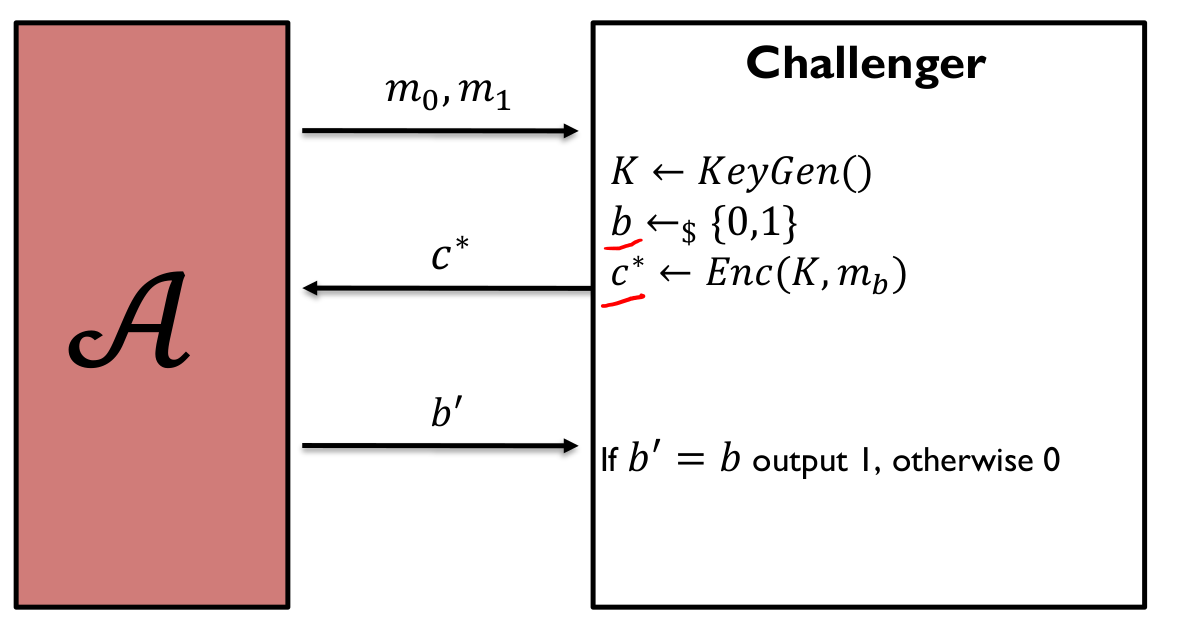
\includegraphics[width=120mm]{Graphics/Perfect Secrecy/def3.png}\newline
				\end{center}
				\begin{itemize}
					\item We call this the ciphertext indistinguishability experiment
				\end{itemize}
    
    	An encryption scheme $(KeyGen,Enc,Dec)$ is perfectly secret, if it holds for \textbf{every adversary} $\mathcal{A}$ that
    	$$Pr[IND_{\mathcal{A}} = 1] = \frac{1}{2}$$
   		where the probability is taken over all random choices of the experiment.\newline
    	\end{definition}
    	
    	\begin{theorem}
    		\cref{Def.PerfectSecrecy1}, \cref{Def.PerfectSecrecy2} and \cref{Def.PerfectSecrecy3} of perfect secrecy are equivalent.
    	\end{theorem}
    	\begin{proof}
    		Proof concept: $((2) \Rightarrow (1)) \rightarrow ((3) \Rightarrow (2)) \rightarrow ((1) \Rightarrow (3))$
    		\begin{itemize}
    			\item[$(2) \Rightarrow (1)$] For all $m,m',c$ show
    					$$Pr[Enc(K,m)=c] = Pr[Enc(K,m')=c] \Rightarrow \delta_{c} := Pr[Enc(K,m)=c]$$
    				Let $M$ be a distribution of messages.
    				Need to show for all $m,c$ that
    					$$Pr[M=m \mid Enc(K,M)=c] = Pr[M=m]$$
    				With Baye's rule it follows, that
    					$$Pr[M=m \mid Enc(K,M)=c] = \frac{Pr[Enc(K,M)=c \mid M=m] \cdot Pr[M=m]}{Pr[Enc(K,M)=c]}$$
    				Now we consider the changed conditional probability
    					$$Pr[Enc(K,M)=c \mid M=m] = Pr[Enc(K,m)=c \mid M=m] = Pr[Enc(K,m)=c] = \delta_c$$
    				The denominator can be formed as follows
    				\begin{align*}
    					Pr[Enc(K,M)=c] &= \sum\limits_{m' \in Supp(M)} Pr[Enc(K,m')=c \mid M=m'] \cdot Pr[M=m']\\
    					&= Pr[Enc(K,m')=c] \cdot \sum\limits_{m' \in Supp(M)} Pr[M=m']\\
    					&= \delta_c \cdot \sum\limits_{m' \in Supp(M)} Pr[M=m'] = \delta_c
					\end{align*}
					So it follows 
					$$Pr[M=m \mid Enc(K,M)=c] = \frac{\delta_c \cdot Pr[M=m]}{\delta_c} = Pr[M=m]$$
					
    			\item[$(3) \Rightarrow (2)$] Via contraposition:\\
    				Assume \cref{Def.PerfectSecrecy2} does not hold, i.e. there exist $m,m',c$ so that
    					$$Pr[Enc(K,m)=c] > Pr[Enc(K,m')=c]$$
    				\textbf{Strategy:} Construct $\mathcal{A}$ so that $Pr[IND_{\mathcal{A}}=1] > \frac{1}{2}$
    				\begin{center}
						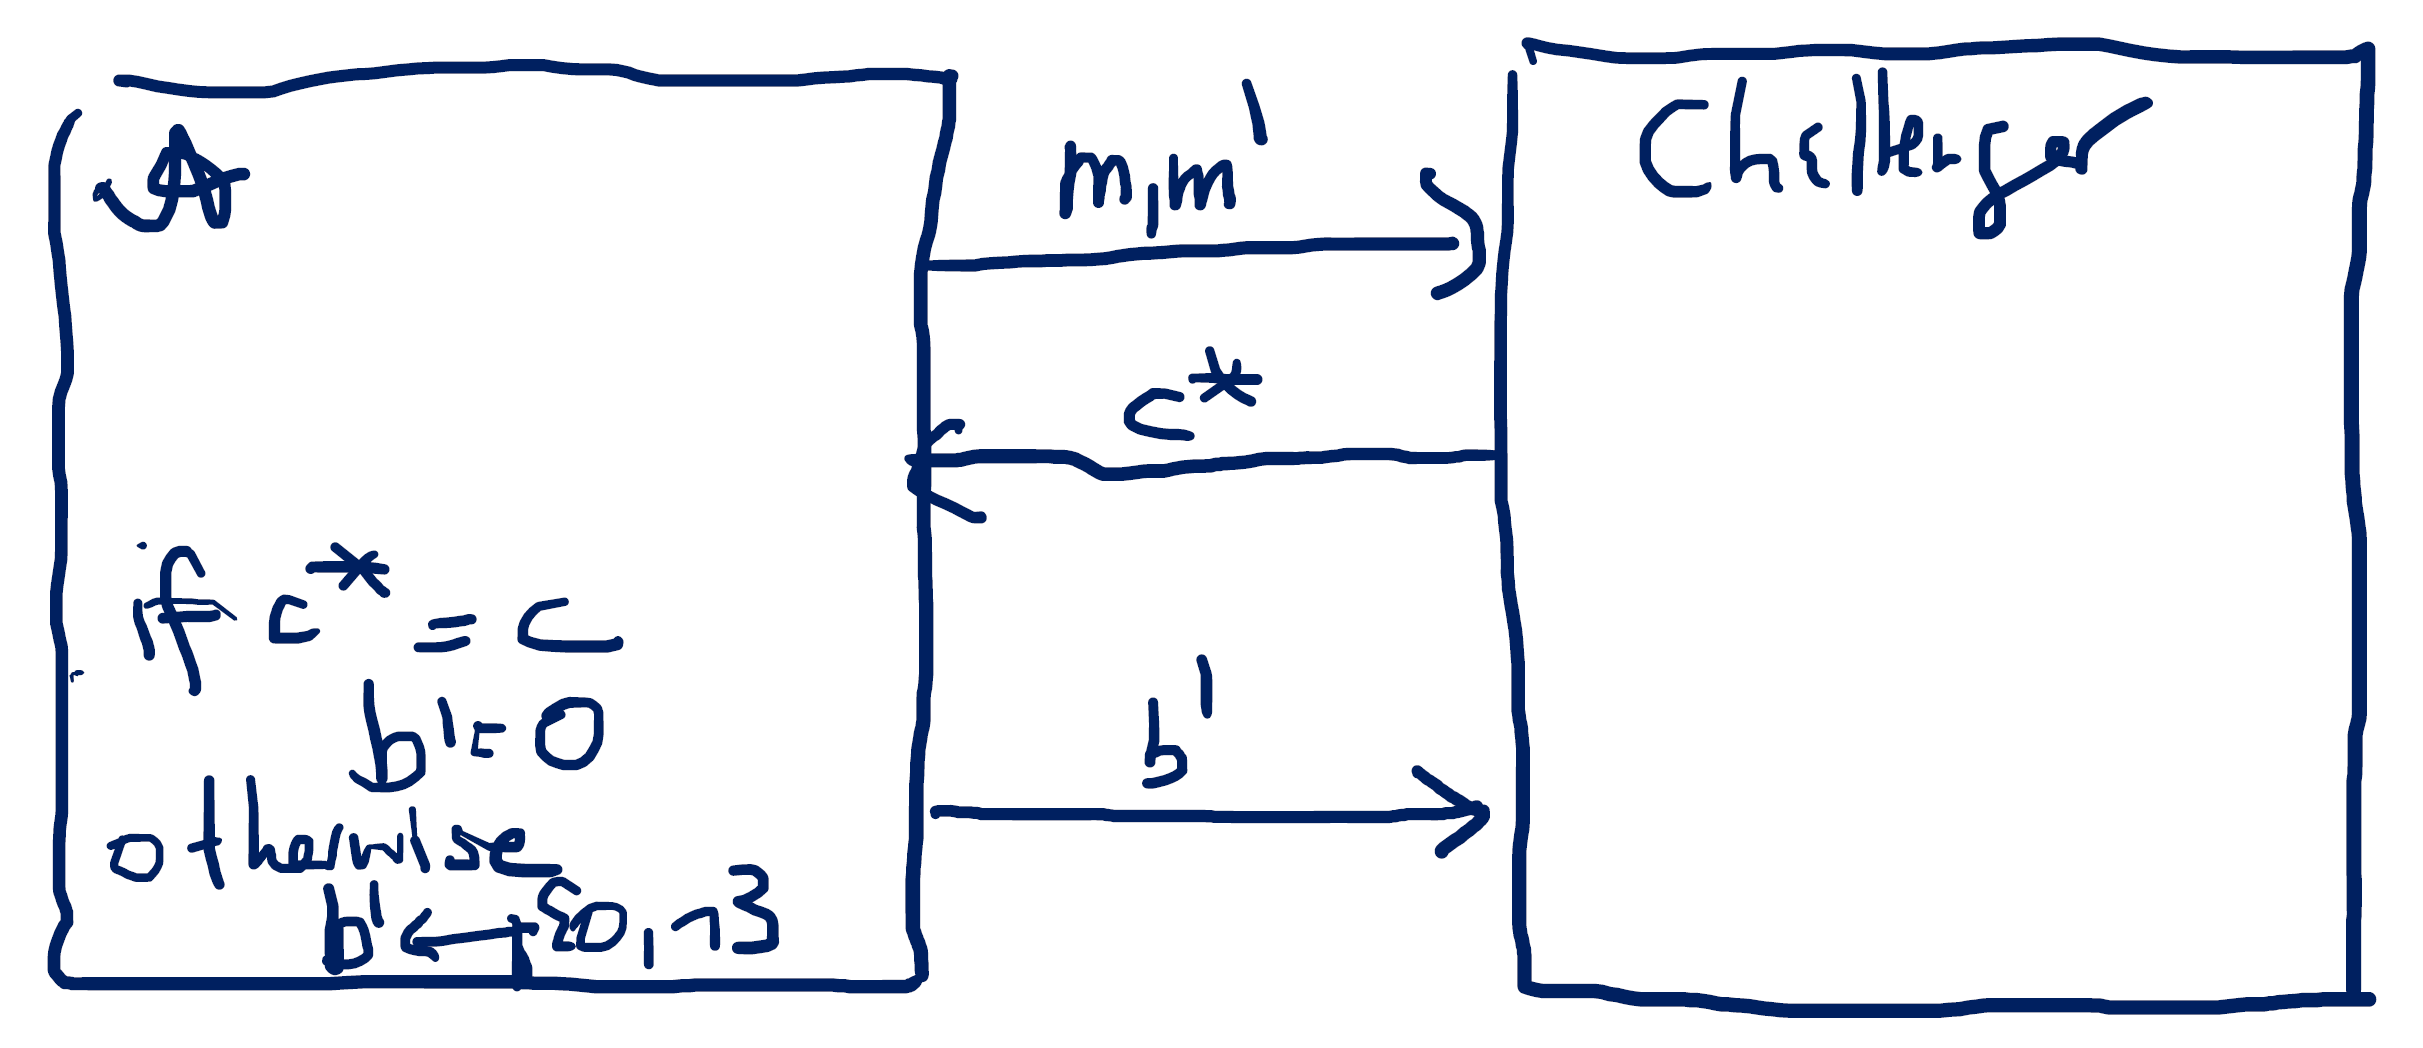
\includegraphics[width=120mm]{Graphics/Perfect Secrecy/Proof(3)to(2).png}\newline
					\end{center}
					with $Pr[c^* = c] > 0$
						$$Pr[Enc(K,m)=c] > Pr[Enc(K,m')=c] \geq 0$$
					With the "law of total probability" it follows that
						$$Pr[IND_{\mathcal{A}}=1] = Pr[IND_{\mathcal{A}}=1 \mid c^*=c] \cdot Pr[c^* = c] + Pr[IND_{\mathcal{A}}=1 \mid c^* \neq c] \cdot Pr[c^* \neq c]$$
					Now we need to show that $Pr[IND_{\mathcal{A}}=1 \mid c^*=c]$:\\
					If $c^* = c$ it holds that $IND_{\mathcal{A}}=1$ if and only if $b=0$\\
					Wherever $c^* = c$ adversary $\mathcal{A}$ will guess $b' = 0$ (by construction)\\
					$\Rightarrow$ Under the condition $c^* = c$ the events $IND_{\mathcal{A}}=1$ and $b=0$ are equivalent.
						$$Pr[IND_{\mathcal{A}}=1 \mid c^* = c] = Pr[b=0 \mid c^* = c]$$
					We will compute $Pr[b=0 \mid c^* = c]$ using Baye's rule and LOTP
						$$Pr[b=0 \mid c^* = c] = \frac{Pr[c^* = c \mid b=0] \cdot Pr[b=0]}{Pr[c^* = c]}$$
					We have to compute two things, first
					\begin{align*}
						Pr[c^* = c \mid b=0] = Pr[Enc(K,m)=c]
					\end{align*}
					and then
					\begin{align*}
						Pr[c^* = c] &= Pr[c^* = c \mid b=0] \cdot Pr[b=0] + Pr[c^* = c \mid b=1] \cdot Pr[b=1]\\
						&= Pr[Enc(K,m)=c] \cdot \frac{1}{2} + Pr[Enc(K,m')=c] \cdot \frac{1}{2}\\
						&= \frac{1}{2} \cdot (Pr[Enc(K,m)=c] + Pr[Enc(K,m')=c])
					\end{align*}
					Now we want to use the results:
					\begin{align*}
						Pr[b=0 \mid c^* = c] &= \frac{Pr[Enc(K,m)=c] \cdot \frac{1}{2}}{\frac{1}{2} \cdot (Pr[Enc(K,m)=c] + Pr[Enc(K,m')=c])}\\
						&= \frac{1}{1 + \frac{Pr[Enc(K,m')=c]}{Pr[Enc(K,m)=c]}} > \frac{1}{2}
					\end{align*}
					with $\frac{Pr[Enc(K,m')=c]}{Pr[Enc(K,m)=c]} < 1$
					
				\item[$(1) \Rightarrow (3)$]
					Let $\mathcal{A}$ be an adversary for the $IND$ experiment.\\
					For now assume that $\mathcal{A}$ is deterministic.
					$\mathcal{A}$ always uses some messages $m_0,m_1$
    				\begin{center}
						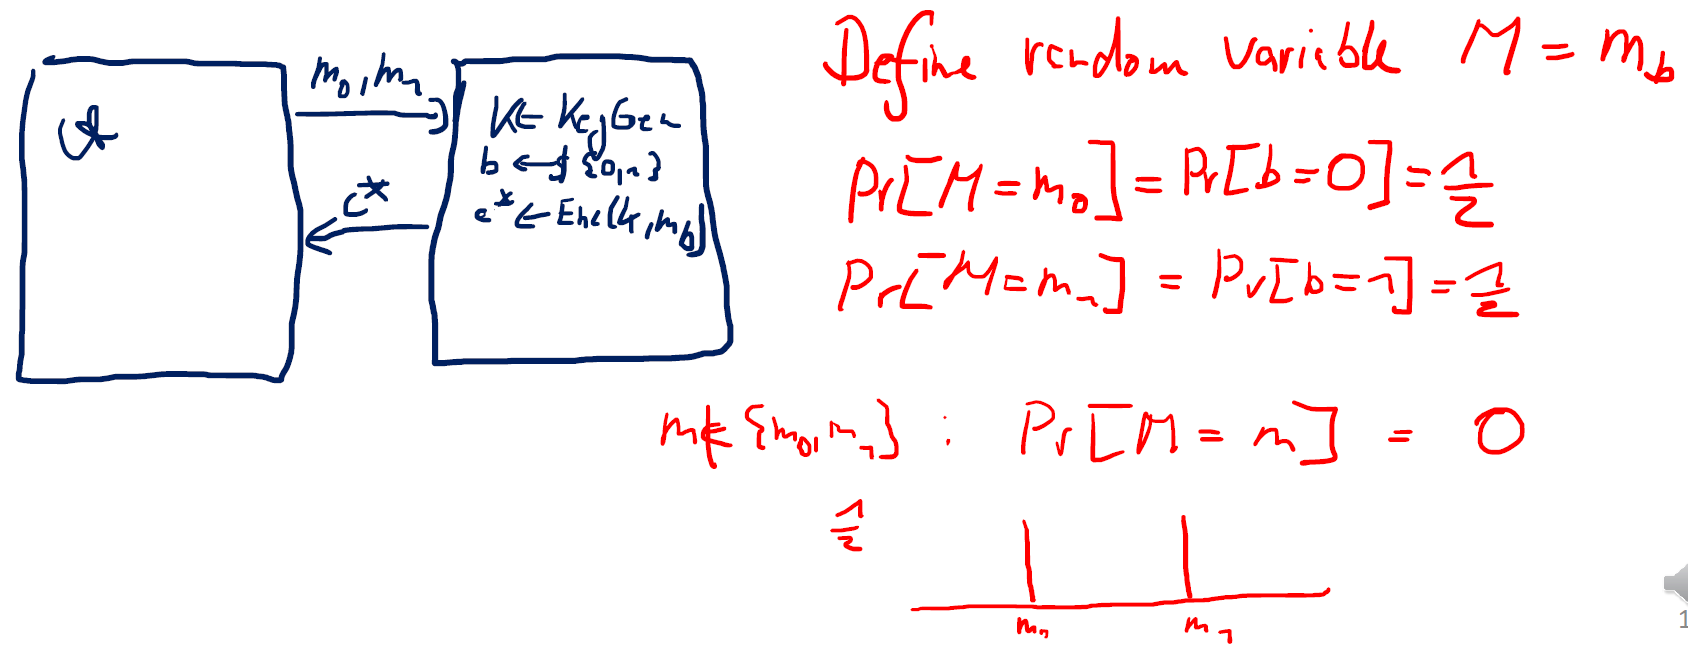
\includegraphics[width=120mm]{Graphics/Perfect Secrecy/Proof(1)to(3).png}\newline
					\end{center}
					So $c^* = Enc(K,m_b) = Enc(K,M)$\\
					\underline{Idea:} Use \cref{Def.PerfectSecrecy1} to show that $c^*$ is independent of $M$ and therefore of $b$\\
					\underline{First:} For $\beta \in \{0,1\}$ the events $M = m_{\beta}$ are equivalent.\\
					For all ciphertexts $c$ it holds:
						$$Pr[b = \beta \mid c^* = c] = Pr[M = m_{\beta} \mid Enc(K,M)=c] = Pr[M = m_{\beta}] = \frac{1}{2}$$
					If we recall that $\mathcal{A}$ is deterministic, we can follow that $b' = b'(c^*)$ is a deterministic function of $c^*$.
					\begin{align*}
						Pr[IND_{\mathcal{A}} = 1] &= Pr[b = b'(c^*)]\\
						&= \sum\limits_{c \in \mathcal{C}} Pr[b = b'(c^*) \mid c^* = c] \cdot Pr[c^* = c] \text{, with LOTP}\\
						&= \sum\limits_{c \in \mathcal{C}} Pr[b = b'(c) \mid c^* = c] \cdot Pr[c^* = c]\\
						&= \sum\limits_{c \in \mathcal{C}} \frac{1}{2} \cdot Pr[c^* = c] = \frac{1}{2} \cdot \sum\limits_{c \in \mathcal{C}} Pr[c^* = c]\\
						&= \frac{1}{2} \cdot 1 = \frac{1}{2}
					\end{align*}
					But what about randomized $\mathcal{A}$?\\
					$\mathcal{A}$ takes as input additional random coins $r \leftarrow \{0,1\}^l$ and write as $\mathcal{A}(r)$ to make this explicit.\\
					\underline{Idea:} For every fixed $\delta \in \{0,1\}^l$, $\mathcal{A}(\delta)$ is a deterministic algorithm.\\
					That means $Pr[IND_{\mathcal{A}(\delta)} = 1] = \frac{1}{2}$ (*), and it follows with the LOTP that
					\begin{align*}
						Pr[IND_{\mathcal{A}(r)} = 1] &= \sum\limits_{\delta \in \{0,1\}^l} Pr[IND_{\mathcal{A}(\delta)} = 1 \mid r = \delta] \cdot Pr[r = \delta]\\
						&= \sum\limits_{\delta \in \{0,1\}^l} \frac{1}{2} \cdot Pr[r = \delta] \text{, because of (*)}\\
						&= \frac{1}{2} \cdot \sum\limits_{\delta \in \{0,1\}^l} Pr[r = \delta] = \frac{1}{2} \cdot 1 = \frac{1}{2}
					\end{align*}

    		\end{itemize}
    	\end{proof}

	
    \begin{itemize}
    	\item For the one time pad, keys are as large as the message and can only be use once.
    	\item Can we construct perfectly secret encryption with short(er) keys? $\leftarrow$ No!
    \end{itemize}
    
    \begin{theorem}[Shannon's Theorem]
        Let $(KeyGen,Enc,Dec)$ be an encryption scheme with key space $\mathcal{K}$,message space $\mathcal{M}$ and ciphertext space $\mathcal{C}$. If it is perfectly secure, then 
        $$\vert \mathcal{K} \vert \geq \vert \mathcal{M} \vert$$
    \end{theorem}
    \begin{proof}
    	Assume $|\mathcal{K}| < |\mathcal{M}|$\\
    	\underline{Strategy:} Show there exist $m_0,m_1$ and ciphertext $c$ so that
    		$$Pr[Enc(K,m_0) = c] > 0$$
    		$$Pr[Enc(K,m_1) = c] = 0$$
    	This contradicts \cref{Def.PerfectSecrecy2} of perfect secrecy.\\
    	
    	Fix an arbitrary $m_0 \in \mathcal{M}$, a key $K_0 \in \mathcal{K}$, and set
    		$$c = Enc(K_0,m_0)$$
    	Define the set
    		$$S = \{ Dec(k,c) \mid k \in \mathcal{K} \} \subseteq \mathcal{M}$$
    	$\Rightarrow |S| \leq |\mathcal{K}| < |\mathcal{M}|$\\
    	$\Rightarrow \mathcal{M} \backslash S \neq \emptyset$, i.e. there exist $m_1 \in \mathcal{M} \backslash S$\\
    	
    	We claim there exists no key $K \in \mathcal{K}$ s.t. $c = Enc(K,m_1)$.\\
    	If there was such a $K$, then by correctness of the scheme it holds
    		$$Dec(K,c) = Dec(K,Dec(K,m_1)) = m_1$$
    	$\Rightarrow m_1 \in S$\\
    	Contradiction to the given condition that $m_1 \in \mathcal{M} \backslash S$
    \end{proof}
    
    \section{Summary 2}
    	\begin{itemize}
    		\item Two alternate definitions for perfect secrecy.
    		\item All 3 definitions are equivalent.
    		\item Perfectly secret schemes have keys as large as the message which can only be used once.
    	\end{itemize}
    
    
    \newpage
    
    
    
    
    
    
    
    
    
    
    
    
    
    
    
    
    
    
    
    
    
    
    
    
    
    
    
    
    
    


\part{Private Key Encryption}



\chapter{Basics of Private Key Encryption}
	
	\section{Limitations of Perfectly Secret Encryption}
		\begin{itemize}
			\item Thm of Shannon: In perfectly secret encryption key must be as long as the message and cannot be reused
			\item But: \textbf{Perfect Secrecy is an overkill!}
			\item Relaxation: Only consider adversaries with realistic computational power
			\item Also: \textbf{Is secrecy alone sufficient? What about other attacks?}
		\end{itemize}
		
	\section{Computational Security: Encryption}
		\begin{itemize}
			\item Back to the problem of secrecy with short keys
			\item \textbf{Idea:} Limit the runtime of adversaries
			\begin{itemize}
				\item We will relax the notion of perfect secrecy by considering only \textbf{computationally bounded} adversaries $\mathcal{A}$
				\item Assume that the runtime of adversaries is upper bounded by a realistic upper bound of $T$ operations, in practice often $T = 2^{80}$
			\end{itemize}
		\end{itemize}
	
	\section{Computationally Secure Encryption}
		Let's modify the definition of perfect secrecy to only account for $T$-bounded adversaries
		\begin{definition}[Computationally Secure Encryption: Attempt 1]
			An encryption scheme $(KeyGen,Enc,Dec)$ is $T-IND$ \textbf{secure}, if it holds for \textbf{every $T$-bounded adversary $\mathcal{A}$} that
			$$Pr[IND_{\mathcal{A}} = 1] = \frac{1}{2}$$
		\end{definition}
		
		Proper Definition: $T$-bounded adversaries with advantage $< \epsilon$
		\begin{definition}[Computationally Secure Encryption: Concrete Indistinguishability Security]
			An encryption scheme $(KeyGen,Enc,Dec)$ is $(T,\epsilon)-IND$ \textbf{secure}, if it holds for \textbf{every $T$-bounded adversary $\mathcal{A}$} that
			$$Pr[IND_{\mathcal{A}} = 1] < \frac{1}{2} + \epsilon$$
		\end{definition}
		\begin{center}
			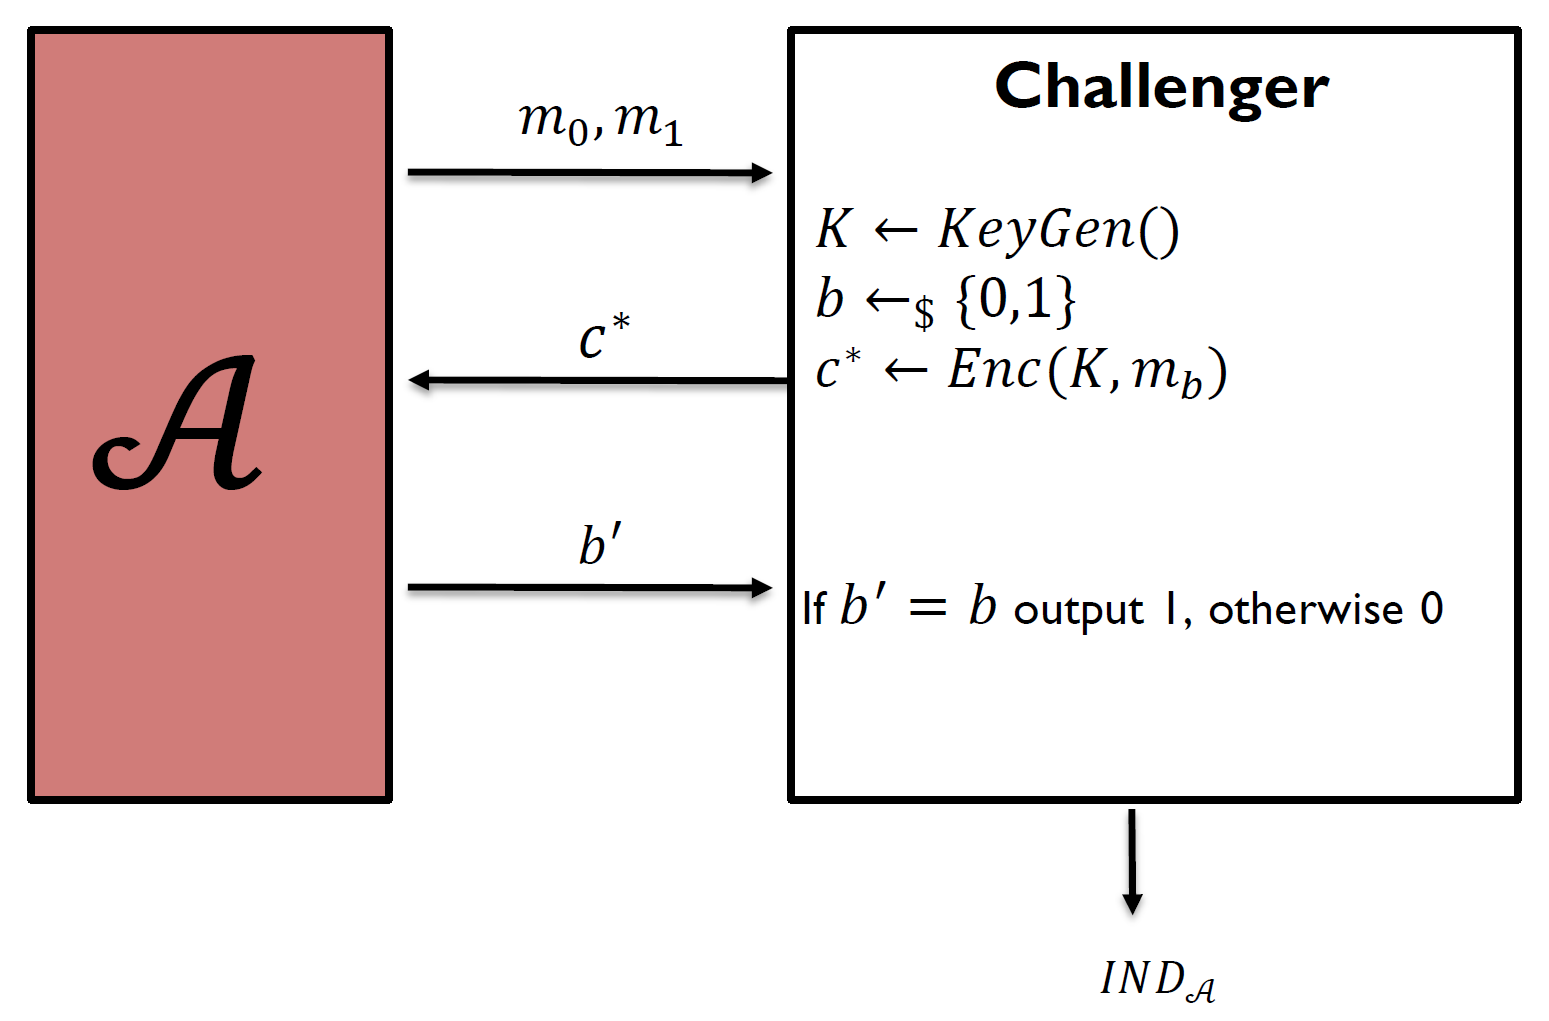
\includegraphics[width=120mm]{Graphics/Basics of Private Key Encryption/ComputationallySecureEncryption.png}\newline
		\end{center}
	
	\section{Concrete Security}
		\begin{itemize}
			\item How do we determine if a scheme is $(T,\epsilon)$-secure?
			\item In practice: Choose parameters of scheme such that \textbf{best known attack} with time complexity $T$ has advantage less than $\epsilon$
			\item In practice, often suggested parameters are $T = 2^{80}$ and $\epsilon = 2^{-60}$
			\item What is the unit of $T$?
			\begin{itemize}
				\item Milliseconds?
				\item Elementary CPU operations?
				\item CPU cycles?
			\end{itemize}
			\item What about other models of computation?
			\item Concrete security is inherently technology dependent!
			\item How can we argue about security in any \textit{reasonable} computational model?
		\end{itemize}
	
	\section{Asymptotic Complexity}
		\begin{itemize}
			\item Computational Complexity Theory!
			\item Recall: In complexity theory problems consist of an infinite number of instances
			\item The complexity of an algorithm solving a problem is measured as a function of the size of an instance, or more generally a \textit{size-parameter}
			\item E.g. sorting: Merge sort has complexity $\mathcal{O}(n \cdot log(n))$ to sort a list of $n$ elements
			\item Recall that we say that an algorithm is efficient, if it runs in time $poly(n)$
		\end{itemize}
		
	\section{Asymptotic Security}
		\begin{itemize}
			\item \textbf{Idea of asymptotic security:} Introduce a security parameter $\lambda$ which characterizes the hardness of breaking a scheme
			\item We only care about what happens when $\lambda \rightarrow \infty$
			\item $KeyGen$ now takes as explicit input security parameter $\lambda$, typically written in unary as $1^{\lambda}$
			\item Efficient computation: \textbf{probabilistic polynomial time (PPT) algorithms}, i.e. randomized algorithms running in time $poly(\lambda)$
			\item Thus efficient adversaries = PPT machines
			\item What about the advantage $\epsilon$?
			\item Exponentially small?
			\item Definitely smaller than $\frac{1}{poly(\lambda)}$ for every polynomial and sufficiently large $\lambda$!
		\end{itemize}

		\begin{definition}[Negligible Functions]
	    	A function $f: \mathbb{N} \to \mathbb{R}_{\geq 0}$ is called negligible, if for every polynomial $p$ there exists an 
	    	$N \in \mathbb{N}$ such that for all $n > N$ it holds that
	    		$$f(n) < \frac{1}{p(n)}$$
	
	    	\textbf{Remark:}
	    	\begin{itemize}
	        	\item It suffices to look at polynomials $p(n) = nˆc$ for constants $c$.
	        	\item We will write $negl(n)$ for an unspecified negligible function.\newline\newline
	    	\end{itemize}
		\end{definition}
		
		\subsection{Examples}
			\begin{itemize}
				\item $f_1(n) = 2^{-n}$ $\rightarrow$ NEGLIGIBLE\\
					because $2^{-n} < n^{-c} \Leftrightarrow -n < -c \cdot log(n) \Leftrightarrow n > c \cdot log(n)$
				\item $f_2(n) = n^{-100}$ $\rightarrow$ NOT NEGLIGIBLE\\
					because $n^{-c} = \frac{1}{n^c}$
				\item $f_3(n) = 2^{-log(n)}$ $\rightarrow$ NOT NEGLIGIBLE\\
					because $2^{-log(n)} = \frac{1}{n}$
				\item $f_4(n) = 2^{-(log(n))^2}$ $\rightarrow$ NEGLIGIBLE\\
					because $2^{-(log(n))^2} < n^{-c} \Leftrightarrow -(log(n))^2 < -c \cdot log(n) \Leftrightarrow (log(n))^2 > c \cdot log(n)$
				\item $f_5(n) = n^{-log(log(n))}$ $\rightarrow$ NEGLIGIBLE\\
					because $n^{-log(log(n))} < n^{-c} \Leftrightarrow log(log(n)) \cdot log(n) > c \cdot log(n)$
				\item \textbf{Simple Rule:} $f$ is negligible iff $-log(f(n)) \geq \omega(log(n))$
			\end{itemize}

		\begin{lemma}[Properties of negligible functions]
	    	If $v_1$, $v_2$ are negligible functions and $p$ is a polynomial, then
	    	\begin{enumerate}
	    	    \item $v_1 + v_2$ is negligible.
	    	    \item $p \cdot v_1$ is negligible.\newline
	    	\end{enumerate}
		\end{lemma}
		\begin{proof}
			Let $q$ be any poly
			\begin{enumerate}
				\item There is at least one $N_1,N_2$ so that:
						$$\forall n > N_1: v_1(n) < \frac{1}{2 \cdot q(n)} \text{ and } \forall n > N_2: v_2(n) < \frac{1}{2 \cdot q(n)}$$
					Let $N = max\{N_1,N_2\}$ be the maximum. So it holds
						$$\forall n > N: v_1(n)+v_2(n) < \frac{1}{2 \cdot q(n)} + \frac{1}{2 \cdot q(n)} = \frac{1}{q(n)}$$
					So it follows that $v_1 + v_2$ is negligible!
				\item Let $q'(n) = p(n) \cdot q(n)$ with $p$ is a polynomial. 
					Then there is at least one $N$ so that:
						$$\forall n > N: v_1(n) < \frac{1}{p(n) \cdot q(n)} \Leftrightarrow p(n) \cdot v_1(n) < \frac{1}{q(n)}$$
					So it follows that $p \cdot v_1$ is negligible!
			\end{enumerate}
		\end{proof}

	\begin{definition}[Encryption Schemes - Full Definition]\ 
    	\begin{itemize}
        	\item \textbf{Syntax:}\\
        	An encryption scheme consists of three PPT algorithms: $(KeyGen,Enc,Dec)$
            	\begin{itemize}
                	\item $KeyGen(1ˆ{\lambda})$: A randomized algorithm which takes as input the security parameter $1ˆ{\lambda}$ (encoded in unary) and outputs a key $K$.
                	\item $Enc(K,m)$: A randomized algorithm which takes a key $K$ and a message $m$ as input and outputs a ciphertext $c$.
                	\item $Dec(K,c)$: A deterministic algorithm which takes as a key $K$ and a ciphertext $c$ as input and outputs a message $m$.
            	\end{itemize}
        	\item \textbf{Correctness:}\newline
            It holds for all $\lambda \in \mathbb{N}$ and all messages $m$ that $Pr[Dec(K,Enc(K,m))=m]=1$, where $K \leftarrow KeyGen(1ˆ{\lambda})$.\newline
    	\end{itemize}
	\end{definition}


	\section{Computationally Secure Encryption: Asymptotic Indistinguishability Security}
		PPT adversaries with negligible advantage
		\begin{definition}[Asymptotic Indistinguishability Security]
	    	An encryption scheme $(KeyGen,Enc,Dec)$ is $IND$-secure, if it holds for every PPT-bounded adversary $\mathcal{A}$ 
	    	there exists a negligible function $v$ s.t. for all $\lambda \in \mathbb{N}$:
	    		$$Pr[IND_{\mathcal{A}}(\lambda)=1] < \frac{1}{2} + v(\lambda)$$
		\end{definition}
		\begin{center}
			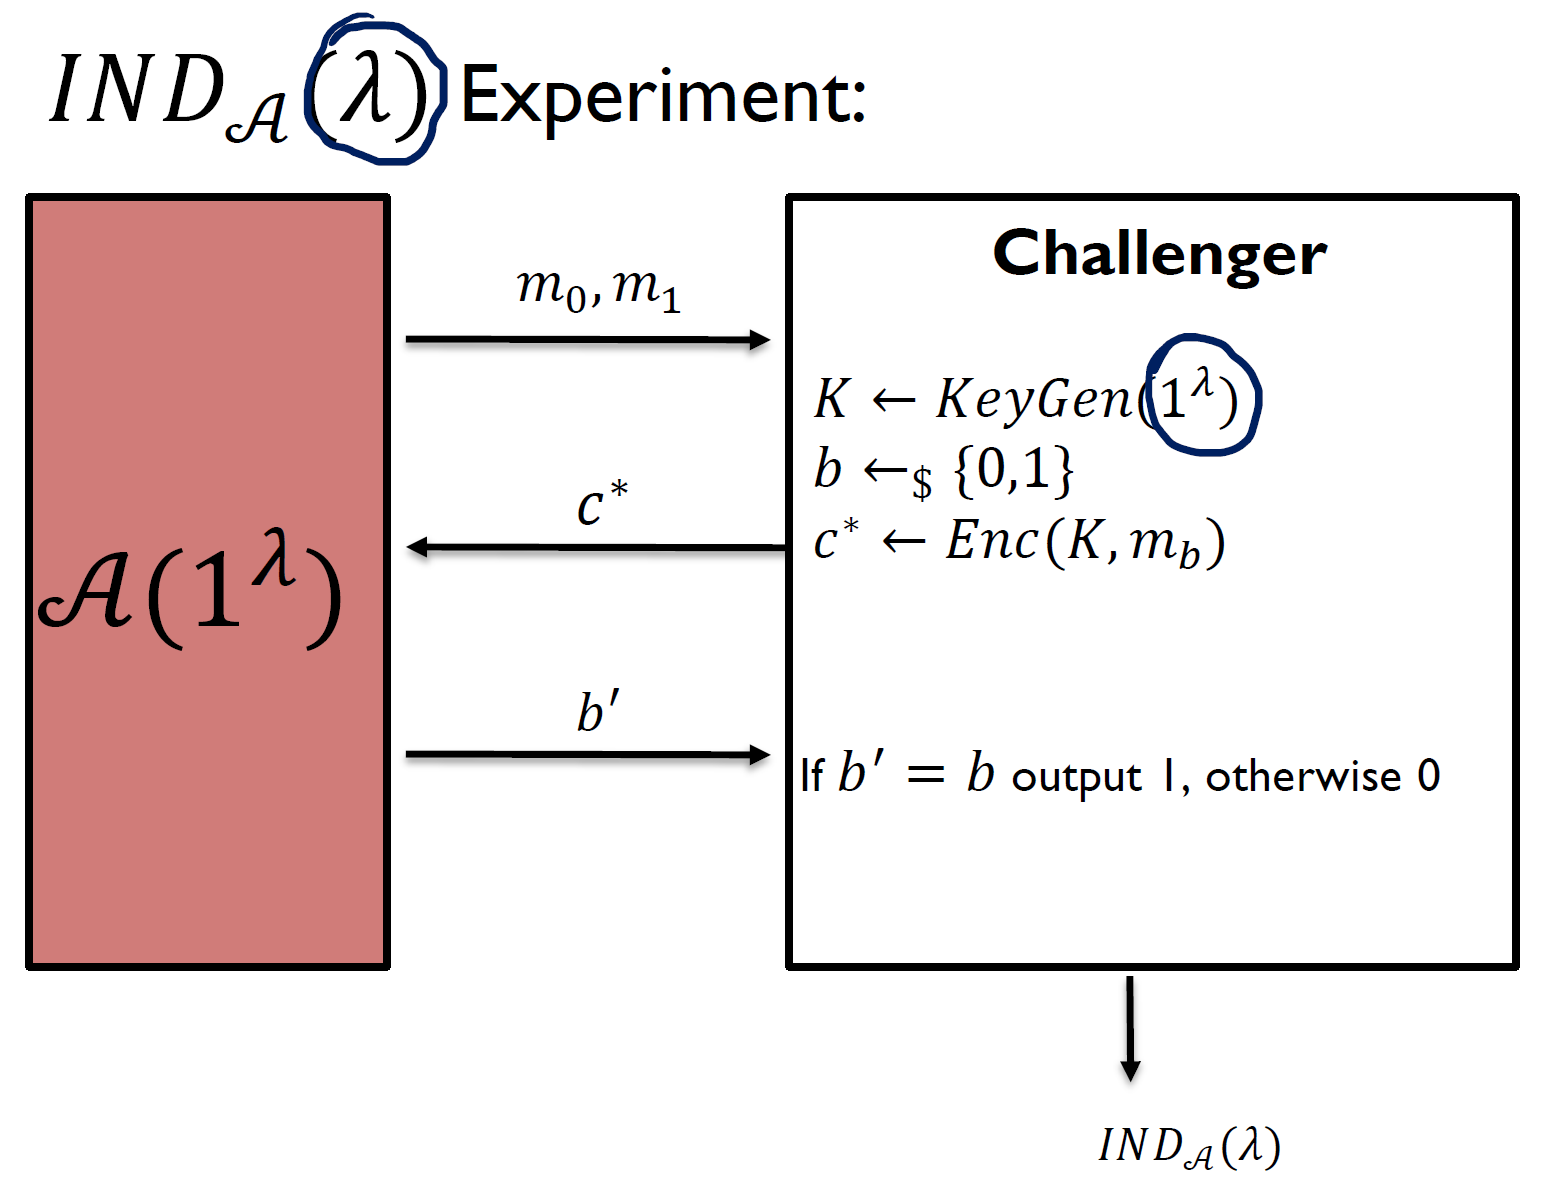
\includegraphics[width=140mm]{Graphics/Basics of Private Key Encryption/AsymptoticIndistinguishabilitySecurity.png}\newline
		\end{center}
	
	\section{Discussion}
		\begin{itemize}
			\item Asymptotic security allows us to base security of schemes on \textbf{standard assumptions} via reductions
			\item Shortcomings: Asymptotic security does not tell us how to instantiate schemes concretely
			\item But: Asymptotic security typically is a guarantee that a scheme has no design flaws.
			\item Attempt at reconciliation: \textit{Tight Security}, i.e. security reductions which provide concrete quantitative guarantees
		\end{itemize}
	
	\section{Summary}
		\begin{itemize}
			\item Perfect security is both an overkill and insufficient
			\item Computational Security: Only consider efficient adversaries, and require their advantage to be small
			\item Asymptotic security: efficient adversaries = \textbf{PPT algorithms}, small advantage = \textbf{negligible advantage}
		\end{itemize}








































\chapter{Stream Ciphers}	
	
	\begin{definition}[Stream Ciphers]\ 
	    \begin{itemize}
	        \item Basic Idea: Take a short key, expand it into a long key and use as one-time pad.
	    \end{itemize}
		\begin{center}
			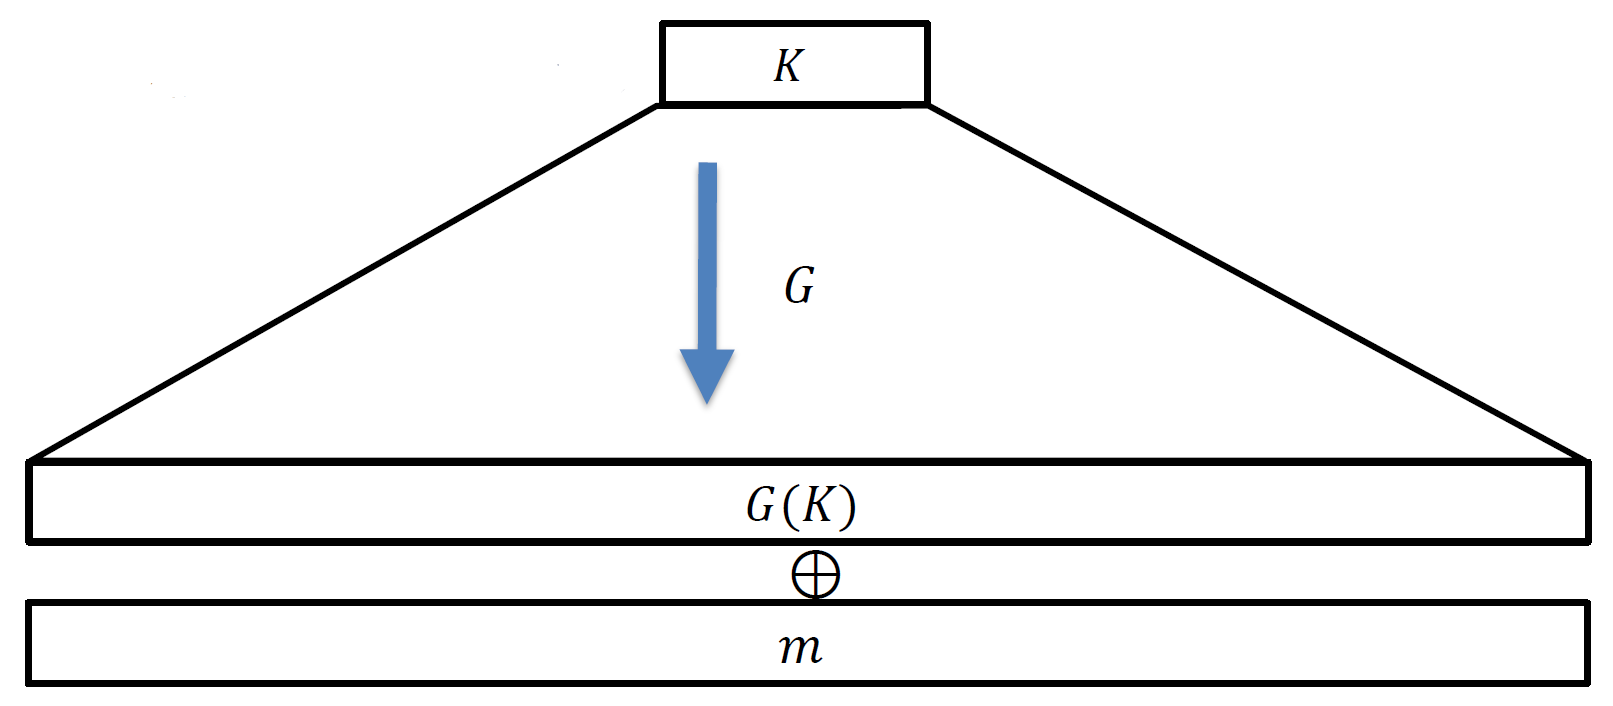
\includegraphics[width=120mm]{Graphics/Basics of Private Key Encryption/StreamCiphers.png}\newline
		\end{center}
		\begin{itemize}
	        \item $KeyGen(1^{\lambda})$: Choose $K \leftarrow_{\$} \{0,1\}^{\lambda}$, output $K$
	        \item $Enc(K,m)$: Compute and output $c \leftarrow G(K) \oplus m$
	        \item $Dec(K,m)$: Compute and output $m \leftarrow G(K) \oplus c$
		\end{itemize}
	\end{definition}
	
	\section{Pseudorandomness against Simple Statistical Tests}
		\begin{itemize}
			\item Idea: $G(K)$ should \textit{behave} like a uniform distribution
			\item Linear Feedback Shift Registers (LFSR)
			\item Un biased: On average same number of $0$'s and $1$'s in output
			\item \textbf{Runs:} On average same number of $0$-runs $000000$ as $1$-runs $111111$
			\item What other \textit{efficient} statistical test should we account for? All of them!
		\end{itemize}
		\begin{center}
			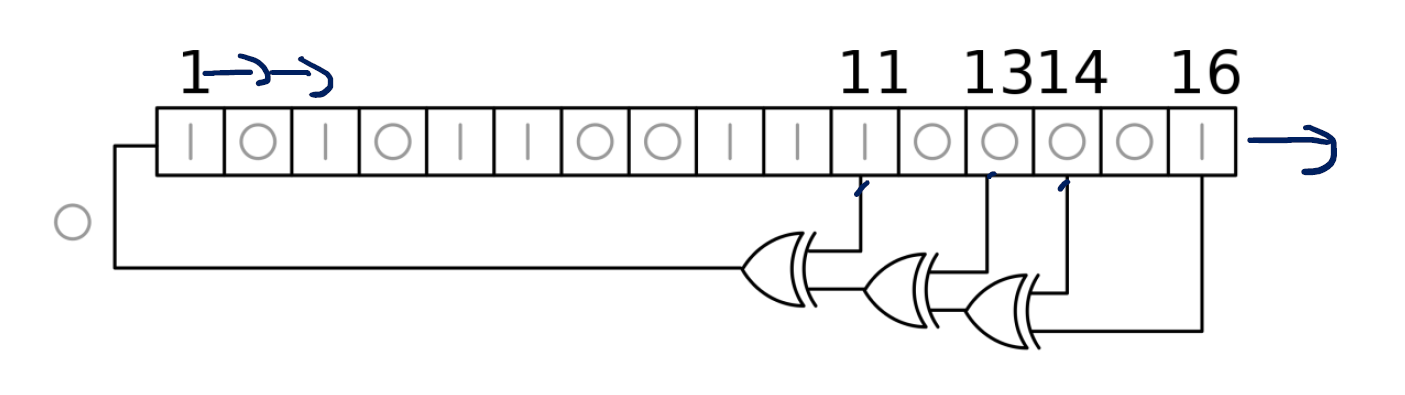
\includegraphics[width=120mm]{Graphics/Basics of Private Key Encryption/PseudorandomnessagainstSimpleStatisticalTests.png}\newline
		\end{center}
	
	\begin{definition}[Pseudorandom Generators]\ 
	    \begin{itemize}
	        \item $G(K)$: deterministic polynomial time algorithm, takes as input $K \in \{0,1\}^{\lambda}$ and outputs $G(K) \in \{0,1\}^l$, where $l = poly(\lambda)$.
	        \item $u$ is uniformly distributed over $\{0,1\}^l$
	        \item A distinguisher is an algorithm which outputs a single bit.
	        \item $G$ is a pseudorandom generator, if it holds for every PPT distinguisher $\mathcal{D}$ that
	            \begin{itemize}
	                \item $\vert Pr[\mathcal{D}(G(k))=1]-Pr[\mathcal{D}(u)=1] \vert \leq negl(\lambda)$
	                \item where probability is over $K \leftarrow \{0,1\}^{\lambda}$, $u \leftarrow \{0,1\}^l$ and the random coins of $\mathcal{D}$.\newline
	            \end{itemize}
	    \end{itemize}
	\end{definition}
	
	\section{Examples}
		\begin{itemize}
			\item Modular Congruence generator:
				\begin{itemize}
					\item $P$ a prime
					\item $\mathbb{Z}_P = \{0,...,P-1\}$
					\item $a,b \leftarrow_{\$} \mathbb{Z}_P$
					\item $x_0 \leftarrow_{\$} \mathbb{Z}_P$
					\item $s = (a,b,x_0)$
					\item $G(s):$ Compute a sequence $x_0,x_1,...,x_l$ via $x_{i+1} \leftarrow a \cdot x_i + b\ mod\ P$
				\end{itemize}
			\item Is this a pseudorandom generator?
				\begin{itemize}
					\item No!
					\item Sequence in completely determined by $x_0,x_1,x_2$
						$$a = \frac{x_2-x_1}{x_1-x_0}\ mod\ P \text{,}\ b = x_1 -a \cdot x_0\ mod\ P$$
						$$x_1 = a \cdot x_0 + b\ mod\ P$$
						$$x_2 = a \cdot x_1 + b\ mod\ P$$
					\item \textbf{Distinguishing attack:} Compute $a,b$ from $x_0,x_1,x_2$ and test for all $i > 2$ if $x_i = a \cdot x_{i-1} + b\ mod\ P$
					\item For a uniform sequence this happens only with probability $P^{-(l-3)}$
					\item Distinguishing advantage: $1-P^{-(l-3)}$
				\end{itemize}
		\end{itemize}
	
	
	\begin{theorem}[Security of Stream Ciphers]\ \\
	    If $G$ is a pseudorandom generator, then $(KeyGen,Enc,Dec)$ is $IND$-secure.
	\end{theorem}
	\begin{proof}
		\textit{Proof by Contraposition:}\\
		Assume $(KeyGen,Enc,Dec)$ is not $IND$-secure\\
		$\Rightarrow$ There is at least one PPT $\mathcal{A}$ and a non-negligible $\epsilon$ so that
		$$Pr[IND_{\mathcal{A}}(\lambda) = 1] = \frac{1}{2} + \epsilon$$
		\begin{center}
			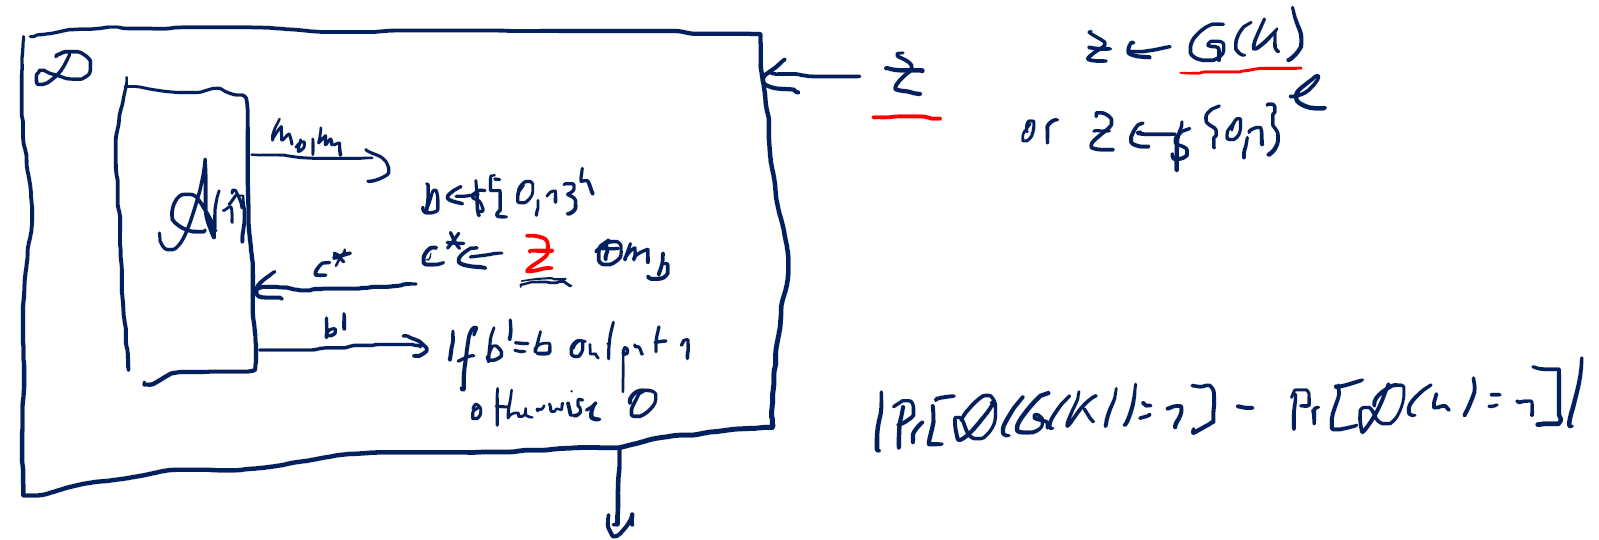
\includegraphics[width=160mm]{Graphics/Stream Ciphers/thm4_1.png}\newline
		\end{center}
		$$Pr[\mathcal{D}(G(K)) = 1] = Pr[IND_{\mathcal{A}}(\lambda) = 1] = \frac{1}{2} + \epsilon$$
		But $Pr[\mathcal{D}(u) = 1] = \frac{1}{2}$ and so it follows, that\\
		$$|Pr[\mathcal{D}(G(K)) = 1] - Pr[\mathcal{D}(u) = 1]| = \frac{1}{2} + \epsilon - \frac{1}{2} = \epsilon$$
		is non-negligible. Therefore $G$ is not a PRG and so the theorem is proven.
	\end{proof}
	
\section{Summary}
	\begin{itemize}
		\item Cryptographic pseudorandom generators (PRGs) need to fool all statistical tests, not just a few we chose
		\item Pseudorandom Generators generate distributions that are far from uniform but cannot be distinguished from uniform by any PPT algorithm
		\item PRGs imply IND secure stream ciphers, for which the key is shorter than the message
	\end{itemize}

	






































\chapter{Chosen Plaintext Security}



\section{Reusing Keys}
	\begin{itemize}
	    \item Stream ciphers have shorter keys than the OTP
	    \item But still keys can only be used once
	    \item How can we make keys reusable?
	    \item First: How should this be modeled in the security definition?
	\end{itemize}
	
	
\section{Chosen Plaintext Attacks}
	\begin{itemize}
	    \item Key-Reuse: Adversary sees many encryptions under the same key
	    \item Not all of them might be unpredictable
	    \item Real Real world scenario: Adversary can influence what honest party encrypts
	    \item Conservative Approach: Let the adversary choose the messages of which he sees encryptions!
	    \item Idea: Give the adversary an \textbf{encryption oracle}
	\end{itemize}
	\begin{center}
		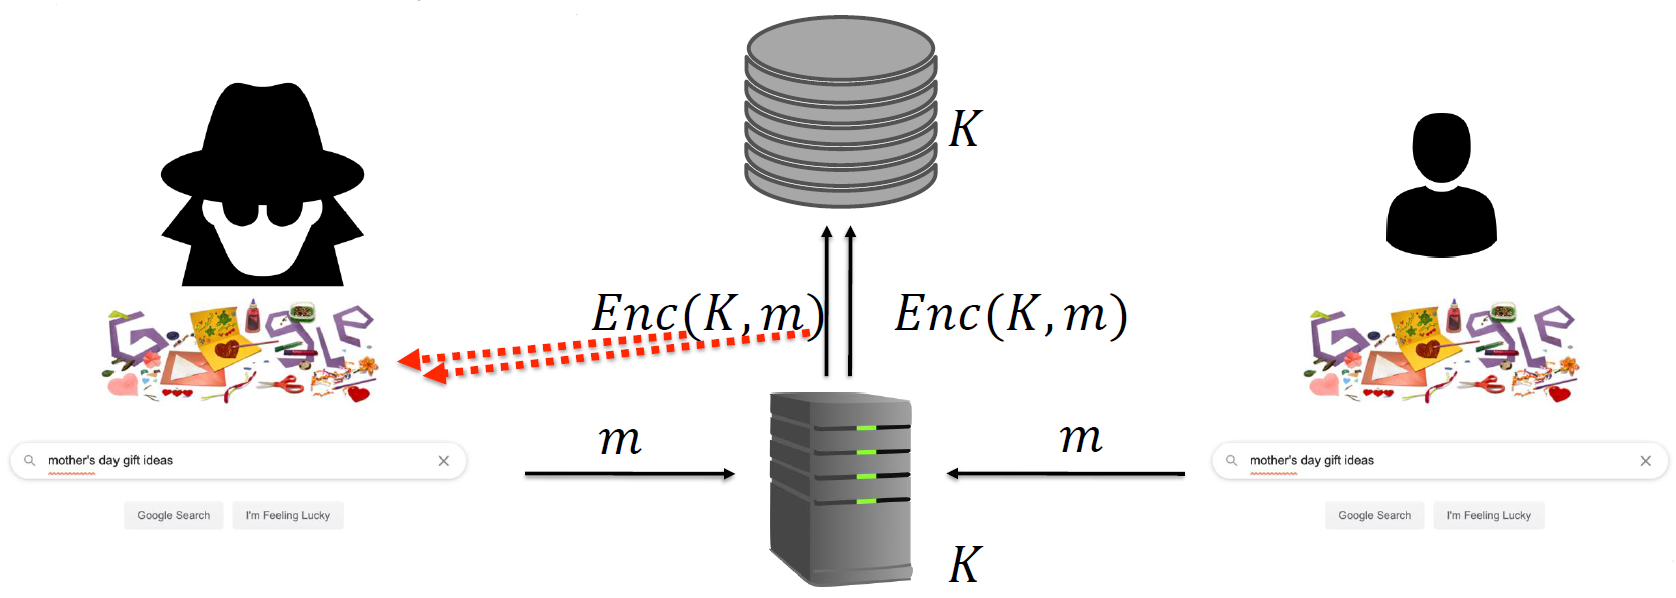
\includegraphics[width=160mm]{Graphics/CPA/cpa1.png}
	\end{center}
	
\newpage
	\begin{definition}[$IND-CPA$-secure]
	    An encryption scheme $(KeyGen,Enc,Dec)$ is $IND-CPA$-secure, if it hol;ds for every $PPT$-adversary $\mathcal{A}$ there exists a negligible function $v$ s.t. 
	    for all $\lambda \in \mathbb{N}$
	    $$Pr[IND-CPA_{\mathcal{A}}(\lambda)=1] < \frac{1}{2} + v(\lambda)$$
	    \begin{center}
			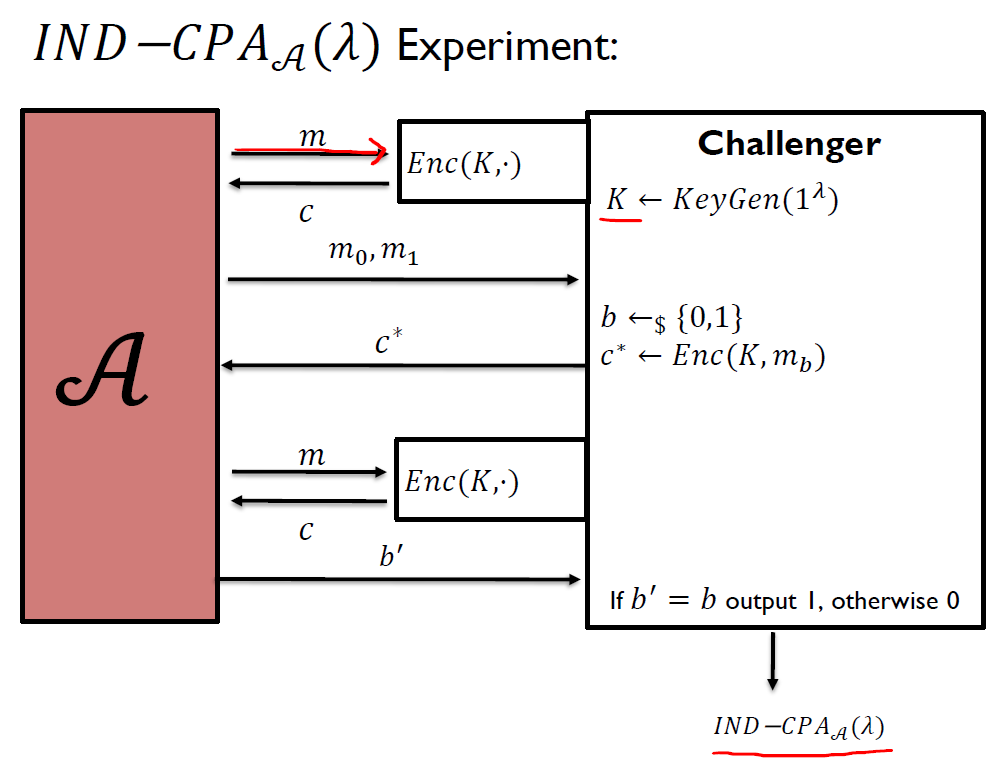
\includegraphics[width=120mm]{Graphics/CPA/cpa2.png}
		\end{center}
	\end{definition}
	
	
	
\section{Constructing IND-CPA secure encryption}
	\begin{itemize}
	    \item Observation: IND CPA secure encryption cannot be deterministic
	    \item Encryption needs to use randomness
	    \item To achieve this stronger security notion, we need stronger ingredient
	    \item PRGs: Small amount of randomness $\Rightarrow$ Larger amount of pseudorandomness
	    \item Needed: Small amount of randomness $\Rightarrow$ (Essentially) unlimited pseudorandomness
	\end{itemize}
	
	
	\begin{definition}[Pseudorandom Functions]\ 
	    \begin{itemize}
	        \item Efficiently computable keyed function (ensemble) $F_K: \{0,1\}^{\lambda} \to \{0,1\}^l$, where $K \in \{0,1\}^{\lambda}$
	        \item Uniformly random function $H: \{0,1\}^{\lambda} \to \{0,1\}^l$
	        \item I.e. for every $x \in \{0,1\}^{\lambda}$ it holds that $H(x)$ is independently uniformly random on $\{0,1\}^l$
	        \item $F$ is a pseudorandom function, if for every oracle PPT distinguisher $\mathcal{D}$ it holds
	        $$\vert Pr[\mathcal{D}^{F_K (\cdot)}(1^{\lambda})=1]-Pr[\mathcal{D}^{H (\cdot)}(1^{\lambda})=1] \vert < negl(\lambda)$$
	        where probability is over choice of $K \leftarrow_{\$} \{0,1\}^{\lambda}$, $H$ and random coins of $\mathcal{D}$.
	    \end{itemize}
	    \begin{center}
			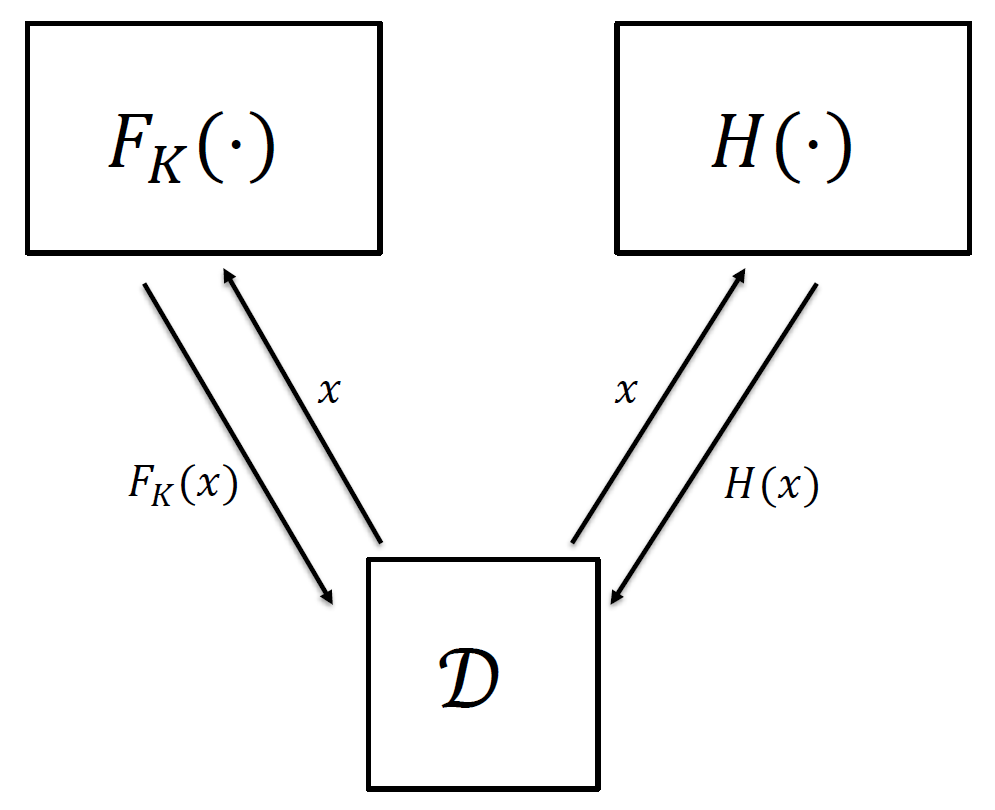
\includegraphics[width=120mm]{Graphics/CPA/prf.png}
		\end{center}
	\end{definition}
	
	
	\subsection{Examples}
		Assume $F, F'$ are PRFs:
		\begin{itemize}
			\item $F^*_{(K,K')}(x) = F_K(x) \oplus F'_{K'}(x)$\\
				$F^*_{(K,K')}(x)$ is a PRF, because
				$${\mathcal{D}^*}^{(F_K \oplus F'_{K'})(\cdot)} \approx {\mathcal{D}^*}^{(H \oplus F'_{K'})(\cdot)} \approx {\mathcal{D}^*}^{H'(\cdot)}$$
				with 
				$${\mathcal{D}^*}^{(F_K \oplus F'_{K'})(\cdot)} \text{ computes } F_K(x) \oplus F'_{K'}(x) \text{, and } 
				{\mathcal{D}^*}^{(H \oplus F'_{K'})(\cdot)} \text{ computes } H(x) \oplus F'_{K'}(x).$$
				Let $H(x)$ be an uniformly random function.\\
				If we XOR a function with an uniformly random function, the result is an uniformly random function too.
				So, $H'(x) := H(x) \oplus F'_{K'}(x)$ is an uniformly random function.\\
				(The proof of reduction was omitted)
			\item $F^*_K (x) = (F_K(x),F_K(x \oplus 1^n))$\\
				$F^*_K (x)$ is not a PRF, because
				$$F^*_K (x \oplus 1^n) = (F_K(x \oplus 1^n),F_K((x \oplus 1^n) \oplus 1^n)) = (F_K(x \oplus 1^n),F_K(x \oplus 1^n \oplus 1^n)) = (F_K(x \oplus 1^n),F_K(x))$$
				has the same output as $F^*_K(x)$ if we change the positions of the tupel.\\
				Therefore the outputs for the inputs $x$ and $x \oplus 1^n$ are correlated. 
		\end{itemize}
	
	
\section{Encryption from Pseudorandom Functions}
	\begin{center}
		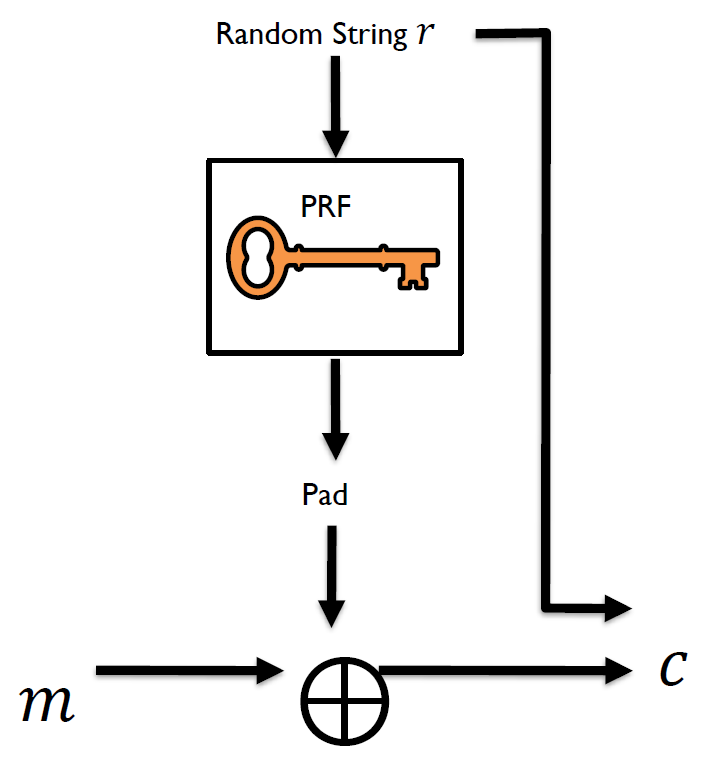
\includegraphics[width=48mm]{Graphics/CPA/cpa3.png}
	\end{center}
	\begin{itemize}
	    \item $KeyGen(1^{\lambda})$: Choose $K \leftarrow_{\$} \{0,1\}^{\lambda}$
	    \item $Enc(K,m)$: Choose $r \leftarrow_{\$} \{0,1\}^{\lambda}$, compute and output $c \leftarrow (r,F_K(r) \oplus m)$
	    \item $Dec(K,c)$: Parse $c=(r,y)$, compute and output $m \leftarrow F_K(r) \oplus y$
	    \item \textbf{Correctness:}
	    $$Dec(K,Enc(K,m))=Dec(K,(r,F_K(r) \oplus m))=F_K(r) \oplus F_K(r) \oplus m = m$$
	\end{itemize}
	
	
	\begin{theorem}[IND-CPA Security]\ 
		\begin{center}
			$F$ is a pseudorandom function $\Rightarrow$ $(KeyGen,Enc,Dec)$ is IND-CPA secure
		\end{center}
	\end{theorem}
	\begin{proof}
		Assume towards contradiction there exists a PPT $\mathcal{A}$ and a non-negligible $\epsilon$ so that
		$$Pr[IND-CPA_{\mathcal{A}}(\lambda) = 1] \geq \frac{1}{2} + \epsilon$$
		\underline{Show:}
		This implies distinguisher $\mathcal{D}$ against PRF $F$ with non-negligible advantage.\\
		First, a thought experiment. What if we use instead of an encryption scheme with a PRF
		$$Enc(K,m) = (r, F_K(r) \oplus m),$$
		a modified encryption scheme with an uniformly random function
		$$Enc'(m) = (r, H(r) \oplus m).$$
	    \begin{center}
			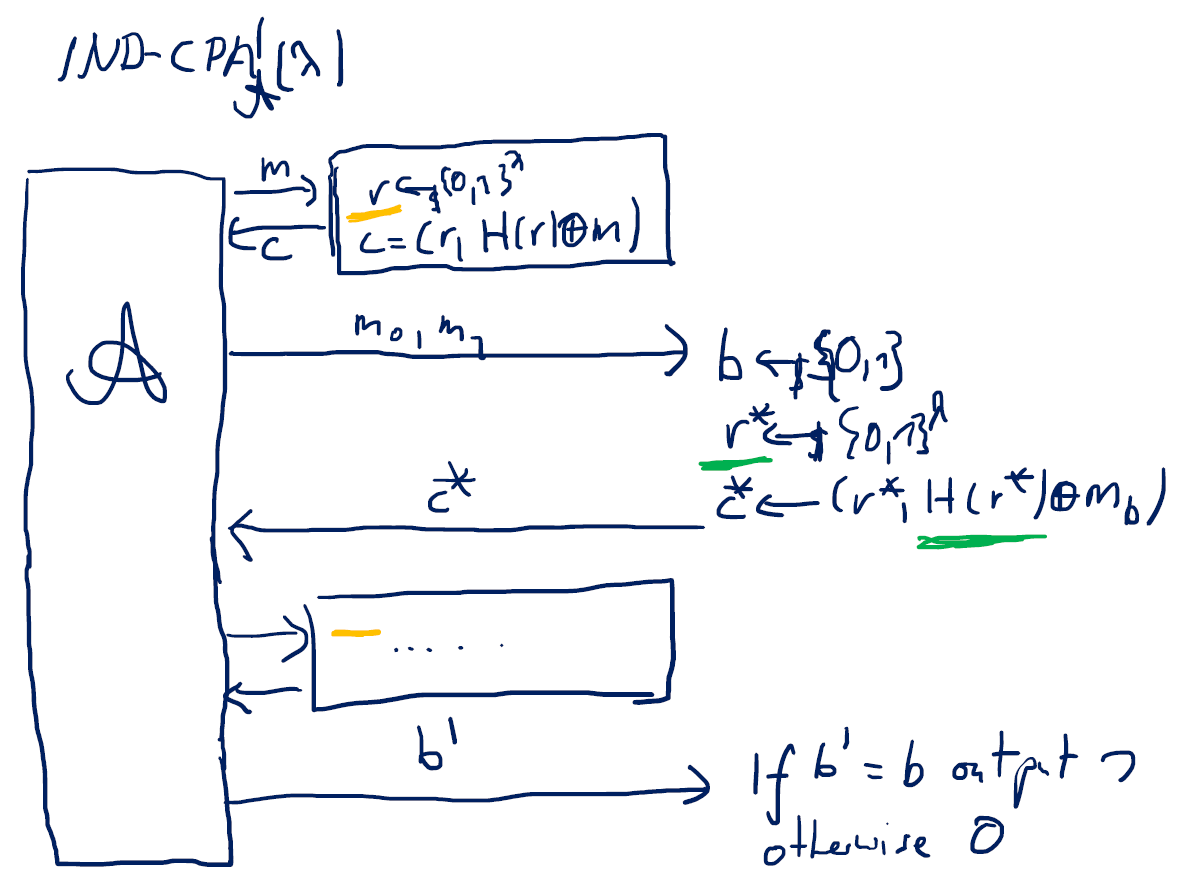
\includegraphics[width=110mm]{Graphics/CPA/cpa4.png}
		\end{center}
		How many r? $\mathcal{A}$ is PPT-machine. It runs in polynomial time.\\
		$\Rightarrow$ Let $q=q(\lambda)=poly(\lambda)$ is an upper bound on the number of queries to enc-oracle by $\mathcal{A}$.\\
		Let $R \subseteq \{0,1\}^{\lambda}$ be the set of strings $r$ used by enc-oracle during the interaction with $\mathcal{A}$.\\
		$\Rightarrow$ $|R| \leq q$
		$\Rightarrow$ $Pr[r^* \in R] = \frac{|R|}{2^{\lambda}} \leq \frac{q}{2^{\lambda}}$\\
		With the LOTP it follows that
		\begin{align*}
			Pr[IND-CPA'_{\mathcal{A}}(\lambda) = 1] &= Pr[IND-CPA'_{\mathcal{A}}(\lambda) = 1 \mid r^* \in R] \cdot Pr[r^* \in R]\\
			&+ Pr[IND-CPA'_{\mathcal{A}}(\lambda) = 1 \mid r^* \notin R] \cdot Pr[r^* \notin R]
		\end{align*}
		Let's consider the single components:
		\begin{itemize}
			\item $Pr[IND-CPA'_{\mathcal{A}}(\lambda) = 1 \mid r^* \in R] \leq 1$
			\item $Pr[r^* \in R] \leq \frac{q}{2^{\lambda}}$
			\item $Pr[IND-CPA'_{\mathcal{A}}(\lambda) = 1 \mid r^* \notin R] = \frac{1}{2}$
			\item $Pr[r^* \notin R] \leq 1$
		\end{itemize}
		Therefore we have
		$$Pr[IND-CPA'_{\mathcal{A}}(\lambda) = 1] \leq \frac{1}{2} + \frac{q}{2^{\lambda}}$$
		with $\frac{q}{2^{\lambda}}$ negligible.
	    \begin{center}
			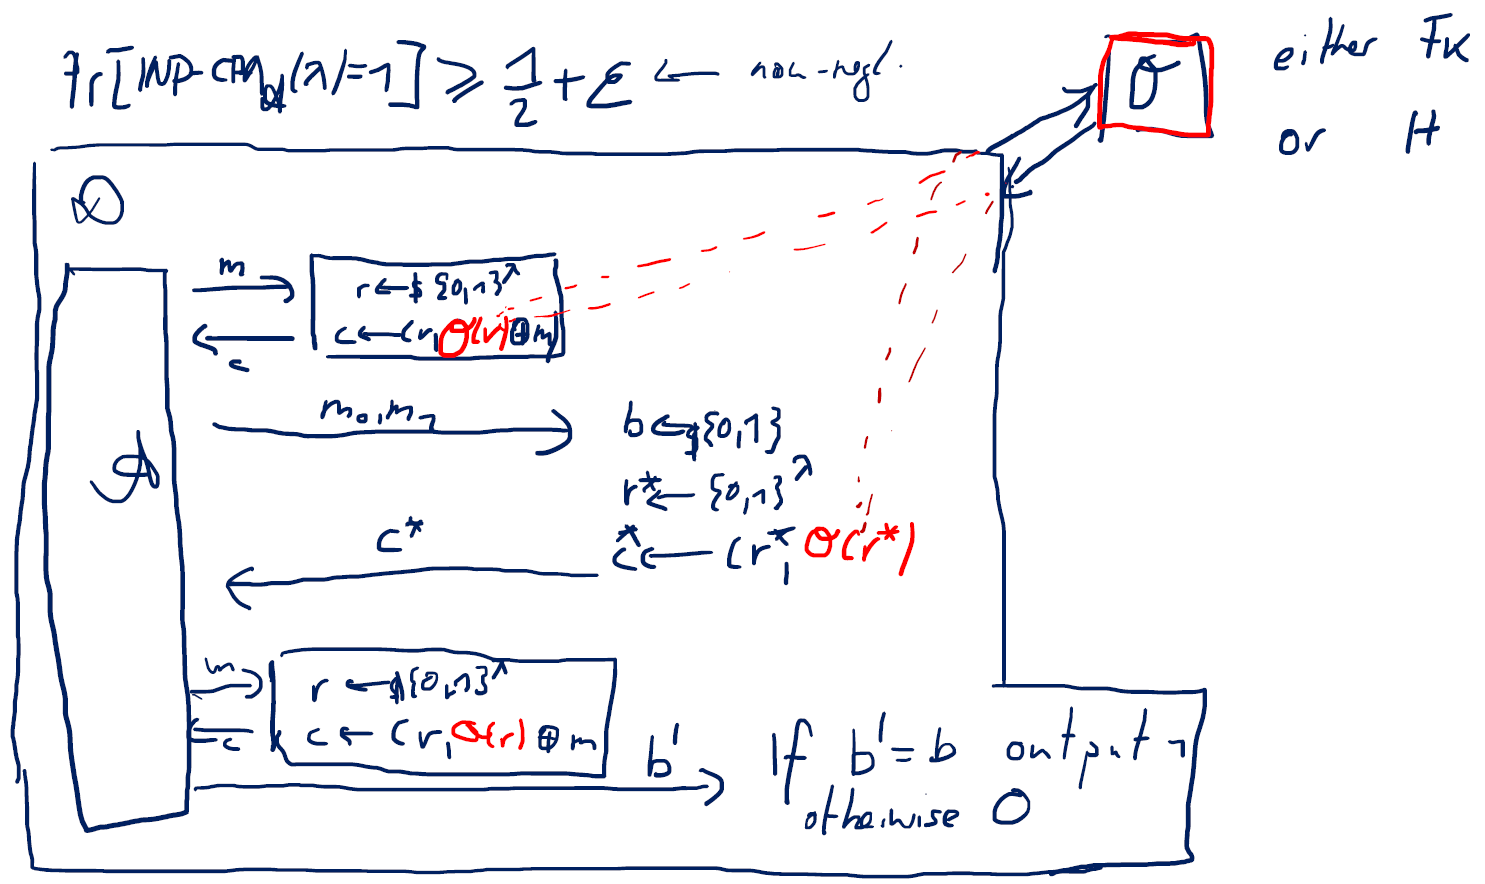
\includegraphics[width=148mm]{Graphics/CPA/cpa5.png}
		\end{center}
		\underline{Case distinction:}
		\begin{enumerate}
			\item If $\mathcal{O} = F_K$ then $\mathcal{D}$ simulates $IND-CPA_{\mathcal{A}}(\lambda)$ experiment:
				$$Pr[\mathcal{D}^{F_K(\cdot)}(1^{\lambda}) = 1] = Pr[IND-CPA_{\mathcal{A}}(\lambda) = 1] \geq \frac{1}{2} + \epsilon$$
			\item If $\mathcal{O} = H$ then $\mathcal{D}$ simulates $IND-CPA'_{\mathcal{A}}(\lambda)$ experiment:
				$$Pr[\mathcal{D}^{H(\cdot)}(1^{\lambda}) = 1] = Pr[IND-CPA'_{\mathcal{A}}(\lambda) = 1] \leq \frac{1}{2} + \frac{q}{2^{\lambda}}$$
		\end{enumerate}
		Now we can follow
		$$Pr[\mathcal{D}^{F_K(\cdot)}(1^{\lambda}) = 1] - Pr[\mathcal{D}^{H(\cdot)}(1^{\lambda}) = 1]
		\geq \frac{1}{2} + \epsilon - \frac{1}{2} - \frac{q}{2^{\lambda}} = \epsilon - \frac{q}{2^{\lambda}}$$
		We know that $\epsilon$ is negligible and $\frac{q}{2^{\lambda}}$ is non-negligible, so it follows that the difference is not negligible! 
	\end{proof}
	
\section{Summary}
	\begin{itemize}
		\item Key reuse requires a stronger security notion: $IND-CPA$ security
		\item $IND-CPA$ secure encryption schemes cannot be deterministic!
		\item $IND-CPA$ secure encryption can be constructed from pseudorandom functions (PRFs)
	\end{itemize}







































\chapter{Block Ciphers}


\begin{definition}[Block Ciphers]\ \\
    Let $k,n$ be positive integers. A block cipher with key length $k$ and block length $n$ is an efficient keyed permutation 
    $$F: \{0,1\}^k \times \{0,1\}^n \to \{0,1\}^n$$
    
    \textbf{Remark:}
    \begin{itemize}
        \item The function $F_K := F(K,\cdot)$ is a bijection (its inverse is denoted $F_K^{-1}$).
        \item Both $F_K$ and $F_K^{-1}$ are efficiently computable given the key $K$.
        \item A secure block cipher should "behave as a pseudorandom permutation".
    \end{itemize}
\end{definition}


\section{A Note on the Concrete Security Setting}
	The key length and block length of block ciphers are fixed $\to$ no varying "security parameter". In practice:
	\begin{itemize}
	    \item actual (not asymptotic) complexity of adversaries is considered.
	    \item a block cipher is considered secure as long as no attack significantly faster than exhaustive key search exists.
	\end{itemize}


\section{Security Definition - Indistinguishability from a Random Permutation}
	\begin{definition}[$(q,t,\epsilon)$-prp secure]\ \\
	    A block cipher $F$ with key length $k$ and block length $n$ is $(q,t,\epsilon)$-prp secure if, for every probabilistic adversary $D$ 
	    that runs in time at most $t$ and deals at most $q$ oracle queries, one has
	    $$Adv_F^{prp}(D) := \vert Pr[D^{F_K(\cdot)}=1]-Pr[D^{f(\cdot)}=1] \vert \leq \epsilon,$$
	    where the first probability is taken over the uniformly random draw of $K$ and the second one over the uniformly random draw of the permutation $f: \{0,1\}^n \to \{0,1\}^n$.
	\end{definition}

	\begin{definition}[$(q,t,\epsilon)$-sprp secure]\ \\
	    A block cipher $F$ with key length $k$ and block length $n$ is $(q,t,\epsilon)$-sprp secure if, for every probabilistic adversary $D$ 
	    that runs in time at most $t$ and deals at most $q$ oracle queries, one has
	    $$Adv_F^{sprp}(D) := \vert Pr[D^{F_K(\cdot),F_K^{-1}(\cdot)}=1]-Pr[D^{f(\cdot),f^{-1}}=1] \vert \leq \epsilon,$$
	    where the first probability is taken over the uniformly random draw of $K$ and the second one over the uniformly random draw of the permutation $f: \{0,1\}^n \to \{0,1\}^n$.
	\end{definition}
	    \textbf{Remark:}\newline
	    $F$ is considered "secure" as long as $Adv_F^{sprp}(D) \leq c_1 \frac{t/T_F}{2^k} + c_2 \frac{q}{2^n}$, where $c_1$ and $c_2$ 
	    are small constants and $T_F$ is an upper bound on the time required to evaluate $F$.


\section{A word on Provable Security}
	\begin{itemize}
	    \item Typically, the security of block ciphers is not provable.
	    \item The pseudorandomness of a block cipher is actually used as an assumption in security proofs for block cipher-based private-key algorithms.
	    \item To build confidence in the pseudorandomness of a block cipher:
	    \begin{itemize}
	        \item decades of cryptanalysis;
	        \item heuristical arguments of security against particular classes of attacks (generic attacks, differential or linear cryptanalysis, ...).
	    \end{itemize}
	\end{itemize}


\section{Design Principles}
	\begin{itemize}
	    \item Block ciphers should behave as pseudorandom permutations: a 1-bit change in the input should affect every bit of the output (avalanche effect)!
	    \item But block ciphers should be efficient and have a short description.
	    \item Confusion-diffusion paradigm: build a pseudorandom permutation from small random (or random-looking) permutations.
	    \item In practice, the following process, called a round, is applied several times to the input block:
	    \begin{enumerate}
	        \item divide the block in small chunks;
	        \item apply small random-looking permutations (called S-boxes) to each chunk of data (confusion);
	        \item mix the bits of the intermediate value to spread the local changes to the whole block (diffusion); this step 
	        can be a simple reordering of the bits or the application of a more complex (invertible) linear function.
	    \end{enumerate}
	\end{itemize}


\section{Substitution-Permutation Networks}
    \begin{center}
		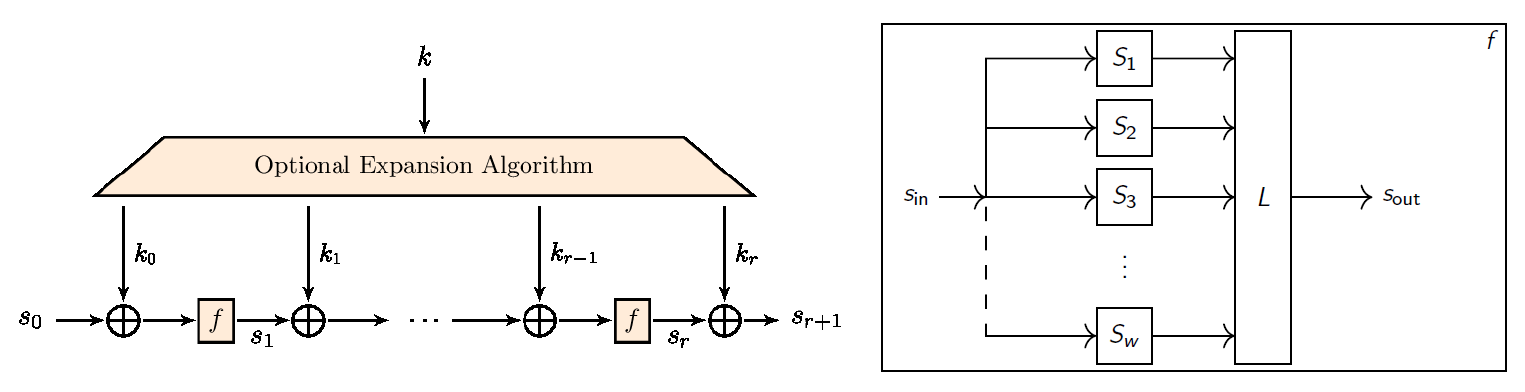
\includegraphics[width=162mm]{Graphics/Block Ciphers/bc1.png}
	\end{center}
	\begin{itemize}
	    \item Practical instantiation of the confusion-diffusion paradigm.
	    \item The S-boxes, key expansion algorithm and linear layer L are public.
	    \item The key is expanded to several subkeys that are mixed with the intermediate values using a bitwise XOR.
	    \item Subkeys are added before each round and after the last one.
	    \item The construction is invertible since both the S-boxes and the linear mixing layer are invertible.
	\end{itemize}


\section{The Avalanche Effect}
	\begin{itemize}
	    \item Example of design criterion to get the avalanche effect:
	    \begin{itemize}
	        \item the S-boxes are chosen so that changing a single bit of the input changes at least two bits of the output.
	        \item the mixing permutations (in that case simple bit reordering) are chosen so that the output bits of any given S-box are used as input of multiple S-boxes in the next round.
	    \end{itemize}
	    \item Consequence:
	    \begin{itemize}
	        \item a single bit difference between input blocks results in a difference of two bits after one round;
	        \item the second condition ensures that the inputs of at least two S-boxes of the second round will differ by one bit;
	        \item after the second round: at least 4 bits differ between the two blocks;
	        \item in the best case, $2^r$ bits will be affected after $r$ rounds (actually less);
	        \item this gives a lower bound for the number of rounds of an SPN: $$r \geq \lceil \log_2(n) \rceil$$
	    \end{itemize}
	\end{itemize}


\section{Feistel Networks}
	\begin{itemize}
	    \item Generic iterated structure to build a PRP from round functions.
	    \item Typically, round functions are also constructed from (possibly non-invertible) S-boxes and linear mixing layers.
	    \item Description of a round:
	    \begin{itemize}
	        \item break the block in two equal halves $L_i$ and $R_i$;
	        \item output $(L_{i+1},R_{i+1})$ defined as $L_{i+1} = R_i$ and $R_{i+1} = L_i \oplus f_i(R_i)$, where $f_i$ denotes 
	        the $i$-th (public) round function instantiated with a (secret) key $K$.
	    \end{itemize}
	    \item Inherently invertible: $R_i = L_{i+1}$ and $L_i = R_{i+1} \oplus f_i(L_{i+1})$.
	\end{itemize}
    \begin{center}
		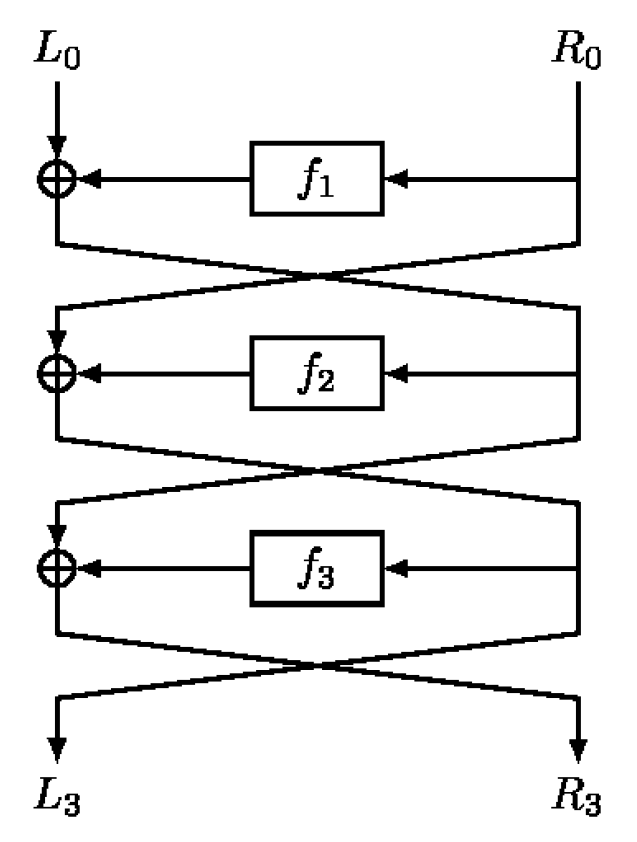
\includegraphics[width=68mm]{Graphics/Block Ciphers/bc2.png}
	\end{center}


\begin{theorem}[Feistel Networks]\ \\
	Assuming the round functions are uniformly random and independent
	functions from $\{0,1\}^n$ to $\{0,1\}^n$, then:
	\begin{itemize}
	    \item the $3$-round Feistel construction is $(q,\infty,\frac{q^2}{2^n})$-prp secure;
	    \item the $4$-round Feistel construction is $(q,\infty,\frac{q^2}{2^n})$-sprp secure;
	    \item the $6$-round Feistel construction is $(q,\infty,\frac{9q}{2^n})$-sprp secure secure as long as $q \leq 2^{n-7}$.\
	\end{itemize}

	\textbf{Interpretation of the theorem:}
	\begin{itemize}
	    \item actual block ciphers have simple round functions that are not random or pseudorandom;
	    \item however, the result justifies the soundness of the Feistel structure;
	    \item it provides lower bounds for the number of rounds that have to be used by an actual block cipher.
	\end{itemize}
	\end{theorem}


\section{Building Blocks of a Block Cipher}
	To summarize, the specification of a block cipher generally contains the following ingredients:
	\begin{itemize}
	    \item a high-level (iterated) structure (SPN, Feistel scheme,. . . );
	    \item a key-schedule algorithm to derive sub-keys from a master key;
	    \item small S-boxes that must be non-linear;
	    \item an efficient linear layer to properly spread local changes from the application of the S-boxes.
	\end{itemize}

\newpage
\section{Examples}
	\subsection{Example 1: The DES Block Cipher}
		\begin{itemize}
			\item DES was developed in the 1970s by IBM (+ some help from the NSA).
			\item Key length: 56 bits and block length: 64 bits.
			\item Although key length is too small for our current standards, it has been impressively resilient to decades of cryptanalysis.
			\item Best cryptanalysis: linear cryptanalysis using $2^{43}$ known plaintext/ciphertext pairs and time around $2^{40}$ DES evaluations.
		\end{itemize}
	    \begin{center}
			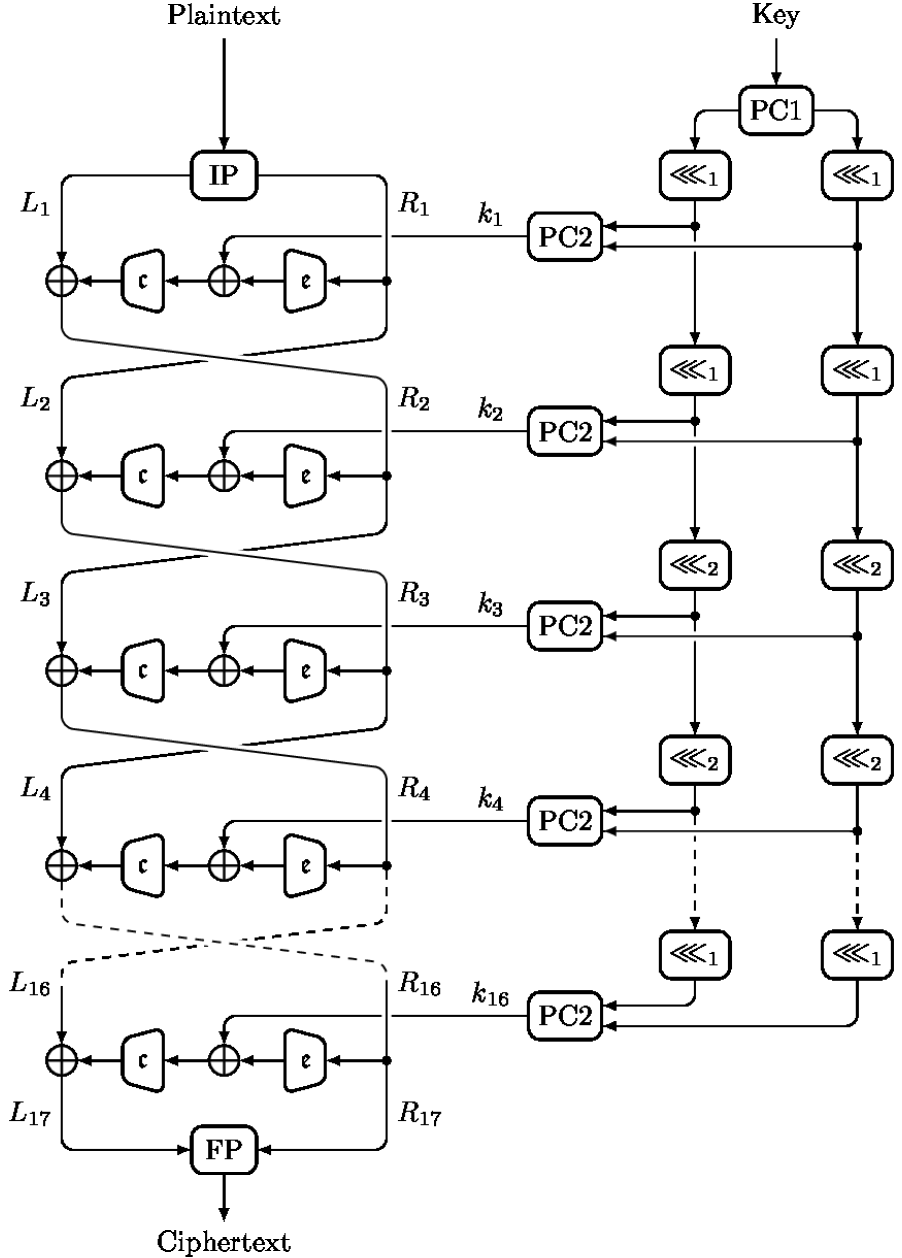
\includegraphics[width=88mm]{Graphics/Block Ciphers/bc3.png}
		\end{center}
		\begin{itemize}
			\item Generic structure: 16 round Feistel network.
			\item Key schedule:
			\begin{enumerate}
				\item PC1 splits the key in two 28-bit halves;
				\item both halves are rotated to the left before each round (number of places depends on the round);
				\item PC2 then extracts 48 key bits.
			\end{enumerate}
			\item IP and FP reorder the bits, but do not depend on any secret information (no impact on security).
			\item Round function:
			\begin{enumerate}
				\item e extends its 32-bit input to 48 bits;
				\item c contracts its 48-bit input back to 32 bits.
			\end{enumerate}
		\end{itemize}
	    \begin{center}
			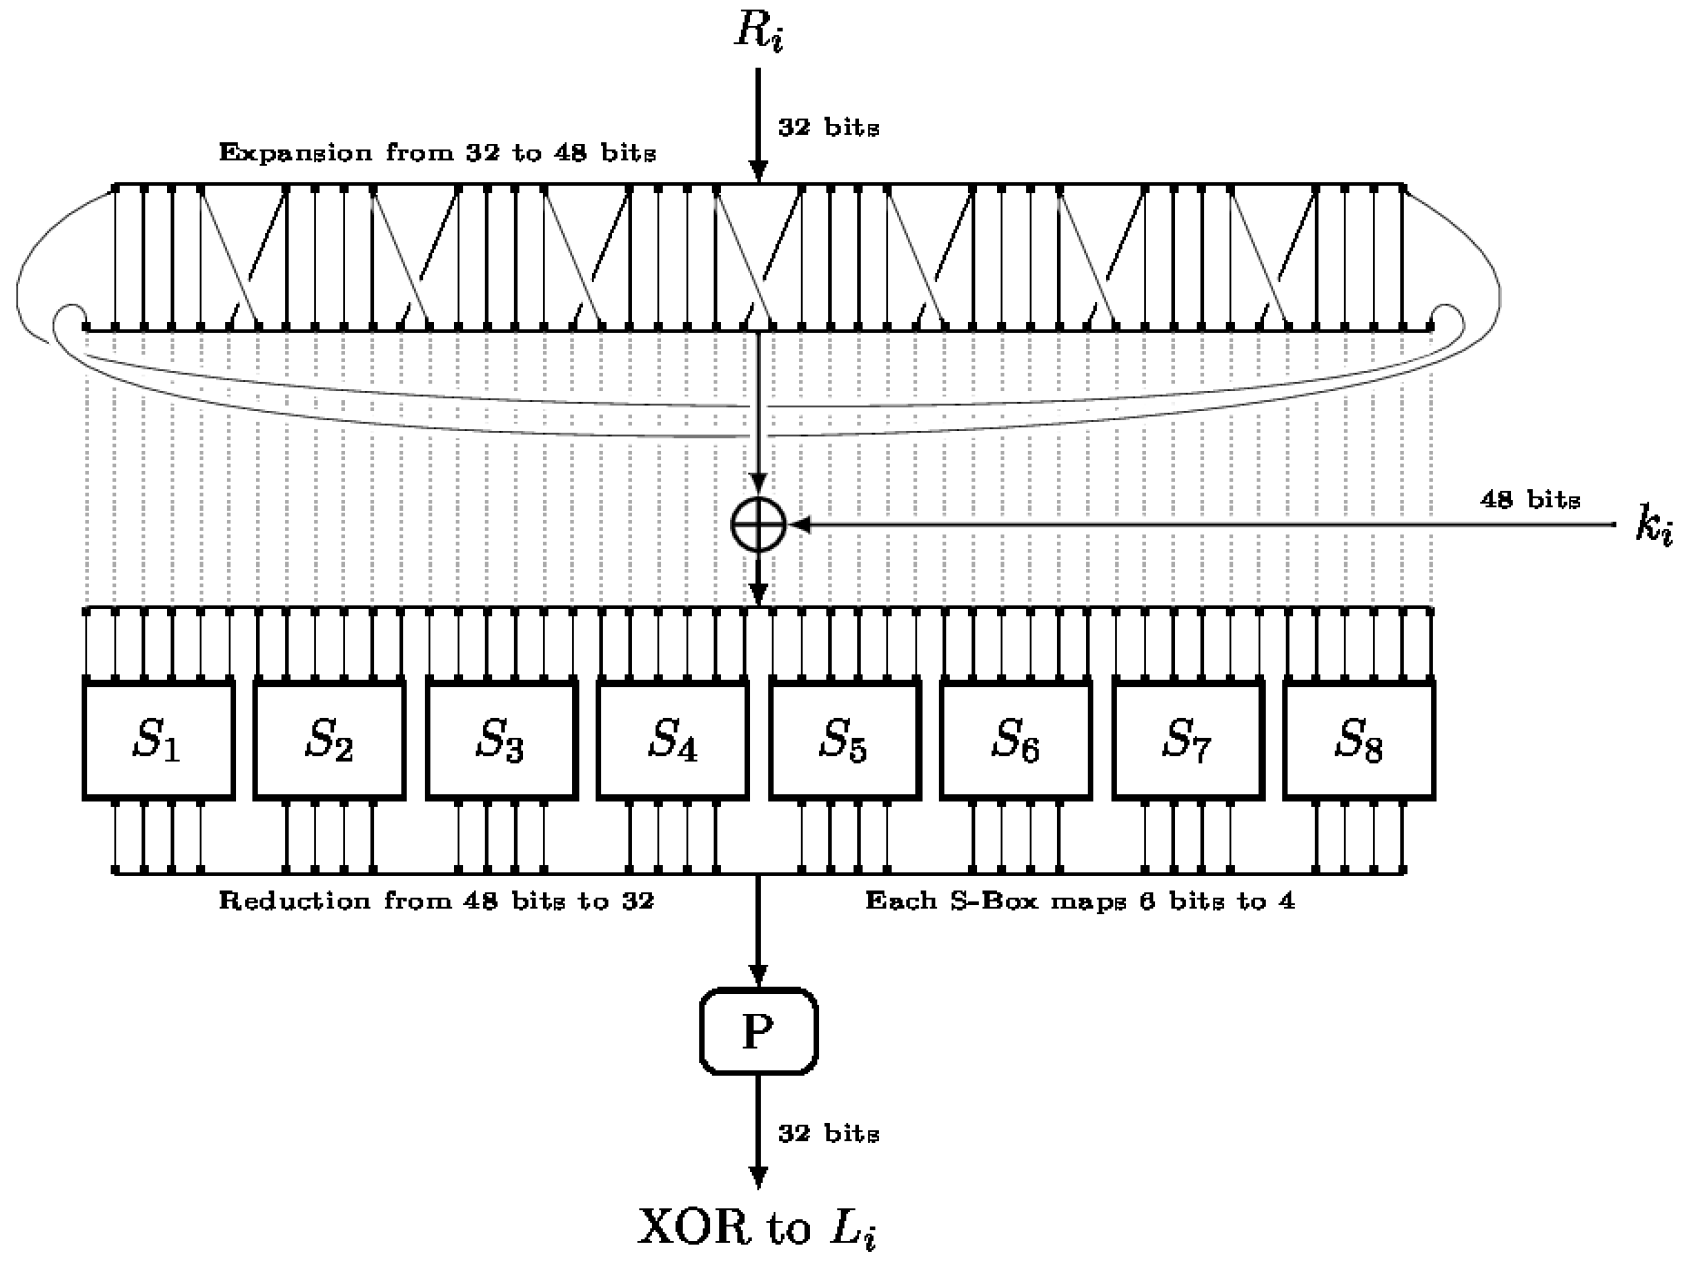
\includegraphics[width=160mm]{Graphics/Block Ciphers/bc4.png}
		\end{center}
		\begin{itemize}
			\item The S-boxes $S_1,...,S_8$ are 6-bit to 4-bit functions such that:
			\begin{enumerate}
				\item each S-box is 4-to-1;
				\item changing one bit of any input to an S-box always changes at least two bits of the output.
			\end{enumerate}
			\item the mixing layer $P$ is a simple reordering of the input bits such that the 4 output bits of any S-box 
			will affect the input to 6 S-boxes in the next round (thanks to the linear expansion layer e).\\
		\end{itemize}
		\textbf{The DES avalanche effect:}
		\begin{enumerate}
			\item Assume $(L_0,R_0)$ and $(L'_0,R'_0)$ are two inputs to the cipher such that $R_0 = R'_0$, $L_0$ and $L'_0$ differ by exactly one bit.
			\item After the first round, since $R_0 = R'_0$, then $L_1 = L'_1$, $R_1$ and $R'_1$ differ by exactly one bit.
			\item Since $L_1 = L'_1$, $R_2$ and $R'_2$ differ by at least 2 bits, while $L_2$ and $L'_2$ differ by exactly one bit.
			\item Thanks to $P$, the 2 different bits of $R_2$ and $R'_2$ appear in at least 2 S-boxes, which means that the new intermediate values will differ in at least 4 positions.
			This results in at least 2 different bits between $L_3$ and $L'_3$ and at least 4 different bits between $R_3$ and $R'_3$.
			\item We observe a similar exponential effect as in the Substitution-Permutation Network case.
		\end{enumerate}

\newpage
	\subsection{The AES Block Cipher}
		\begin{itemize}
			\item United States National Institute of Standards and Technology (NIST) standard adopted in 2000 after an open competition.
			\item Based on the winner of the competition: Rijndael (designed by Vincent Rijmen and Joan Daemen).
			\item Actually a set of 3 algorithms with block length 128 bits and key length 128, 192 or 256 bits.
			\item The length of the key affects the number of rounds (10, 12 or 14) and the key schedule.
			\item Modern processors support instruction sets to accelerate the computation of AES in hardware: around 4.5GB/sec for AES-128 in CTR mode 
			on an Intel(R) Core(TM) i7-3740QM CPU @ 2.70GHz (Fedora 31, openssl 1.1.1d)
			\item Best cryptanalysis: there exist attacks that recover the AES key with a computational complexity of $2^{126}$ operations for AES-128, 
			$2^{189}$ operations for AES-192, and $2^{254}$ operations for AES-256.
			No practical threat to the security of the cipher.
			\item Better attacks exist if the adversary is given more power (the ability to XOR any constant of its choice to the secret key), 
			but this does not impact the security of AES when used in standard modes of operation.
			\item Generic structure: 10, 12 or 14-round Substitution-Permutation Network.
			\item Key schedule: relies on linear operations and on the AES S-box, and outputs one 128-bit sub-key for each round, plus a final one.
			\item The AES round permutation consists in four steps:
			\begin{itemize}
				\item AddRoundKey: the bitwise XOR of the round key;
				\item SubBytes: the application of a single invertible S-box to each of the 16 bytes of the input;
				\item ShiftRows: a reordering of the bytes of the state;
				\item MixColumns: the application of a linear operation to the state.
			\end{itemize}
			\item In the last round, the MixColumns operation is skipped, and replaced with the XOR of the last key.
		\end{itemize}
	    \begin{center}
			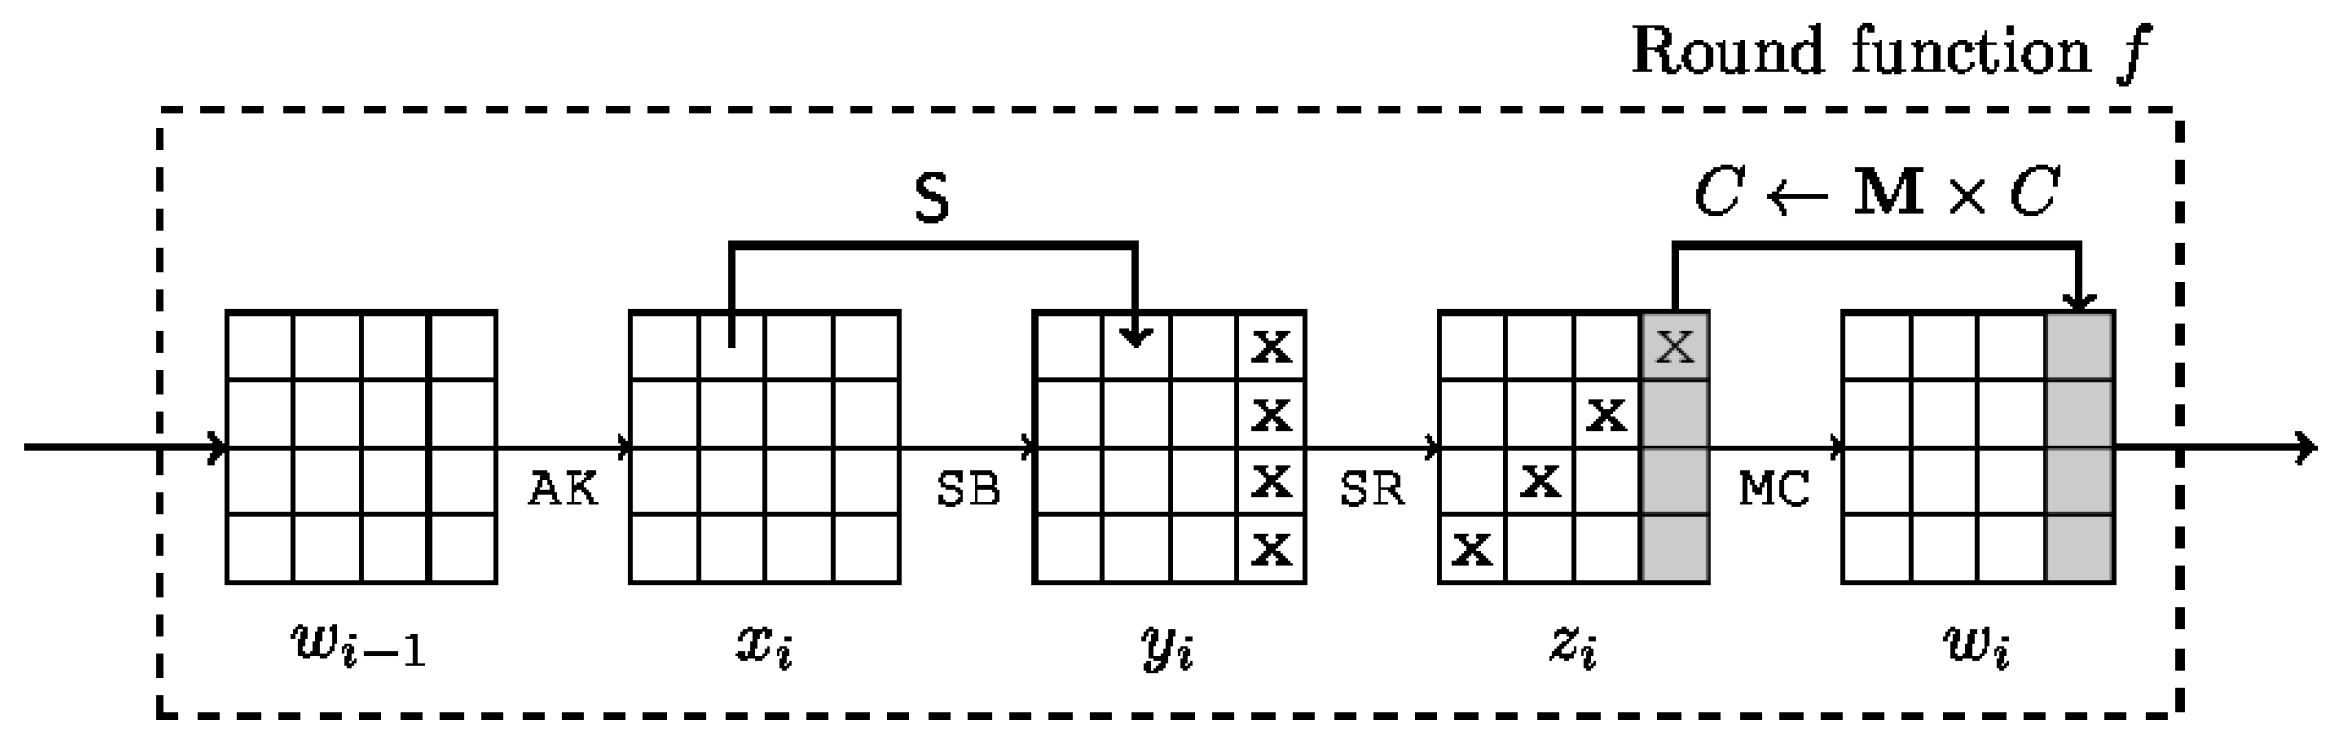
\includegraphics[width=140mm]{Graphics/Block Ciphers/bc5.png}
		\end{center}
		\begin{itemize}
			\item The block is seen as a $4 \times 4$ matrix of bytes.
			\item SubBytes applies the AES S-box to each element of the matrix.
			\item ShiftRows cyclically shifts row $r$ of the matrix by $r$ positions to the left for $r = 0,1,2,3$.
			\item MixColumns can be seen as the multiplication of each column of the matrix by a fixed invertible $4 \times 4$ matrix.
			This transformation has the property that, if two inputs differ in $b > 0$ bytes, then the outputs will differ in at least $5-b$ bytes.
		\end{itemize}
\newpage
		\textbf{The AES avalanche effect:}
		\begin{enumerate}
			\item Assume $X_0$ and $X'_0$ are two inputs to the cipher that differ in exactly one byte.
			\item After the first ShiftRows step, they will still differ in exactly one byte.
			However, at the end of the first round, all the bytes of the corresponding column will differ between both intermediate values, while the remaining bytes will stay equal.
			\item After the second ShiftRows step, there will be exactly one byte per column that will differ between both intermediate values.
			\item At the end of the second round, all bytes will be different between both intermediate values.
		\end{enumerate}

\section{Blockcipher Modes of Operation}
	\subsection{Using Block-Ciphers}
		\begin{itemize}
			\item Block ciphers/PRPs are a \textit{primitive}
			\item How do we construct encryption from PRPs?
			\item Constructions of encryption from block ciphers are called \textbf{modes of operation}
			\item Assume messages can be chopped into blocks of size $\lambda$, otherwise use padding
		\end{itemize}
	    \begin{center}
			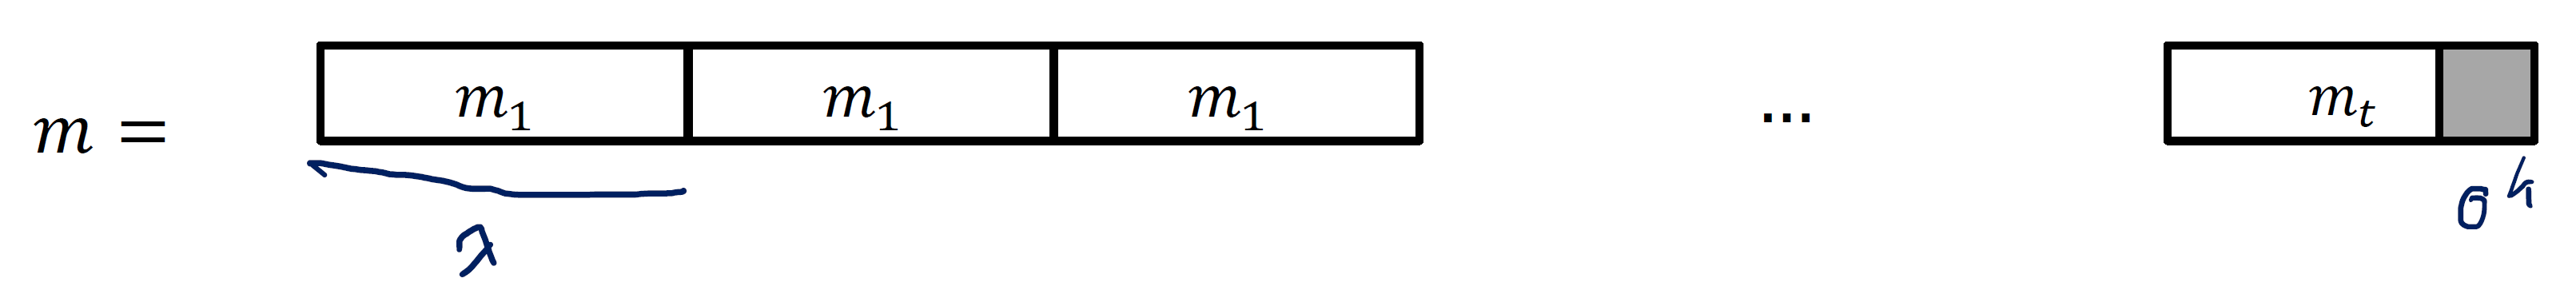
\includegraphics[width=160mm]{Graphics/Block Ciphers/bc6.png}
		\end{center}
	
	\subsection{Electronic Codebook Mode (ECM)}
		\begin{center}
			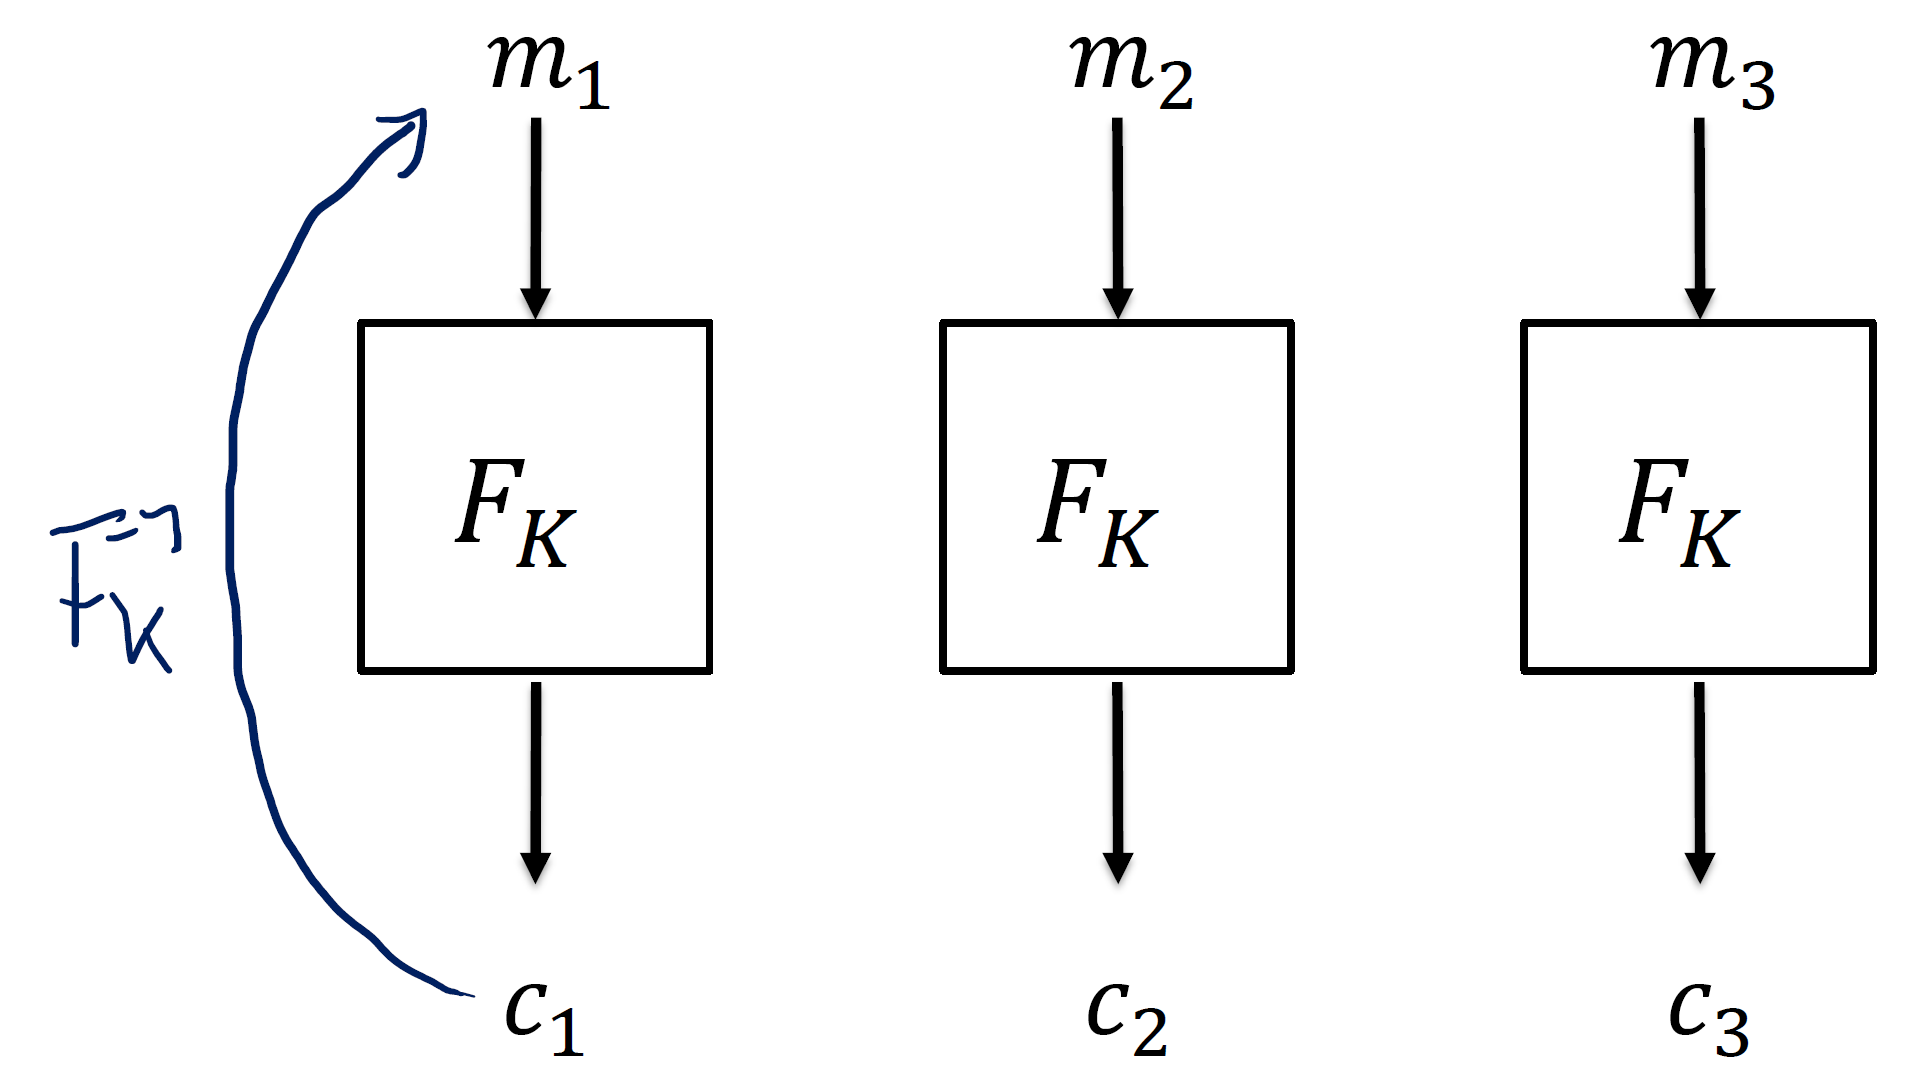
\includegraphics[width=140mm]{Graphics/Block Ciphers/bc7.png}
		\end{center}
		\begin{itemize}
			\item Not IND-CPA secure!
			\item Not even IND secure!
			\item Should not be used!
		\end{itemize}
		\begin{center}
			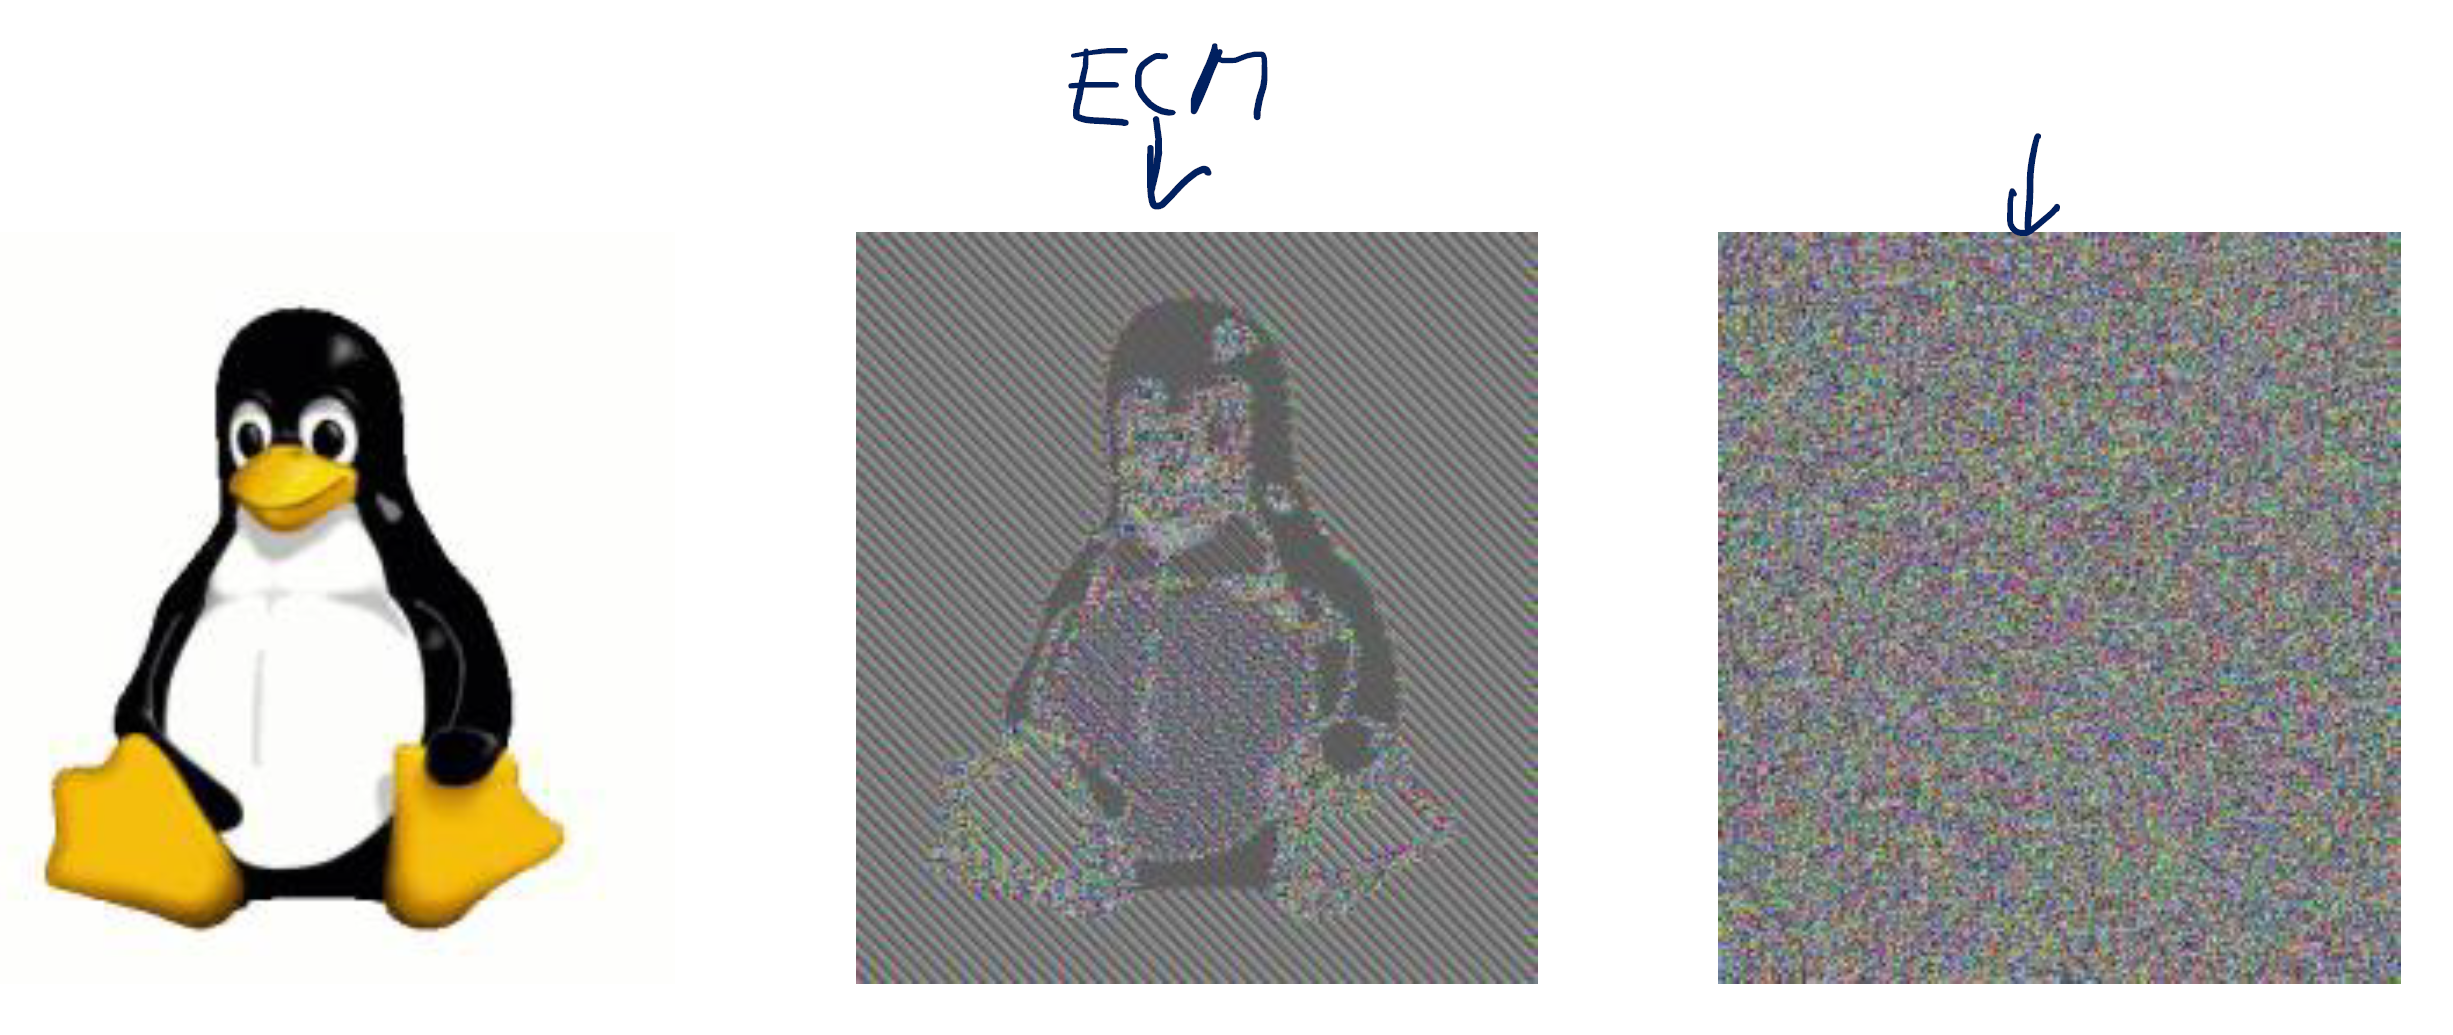
\includegraphics[width=160mm]{Graphics/Block Ciphers/bc8.png}
		\end{center}
	
	\subsection{Cipher Block Chaining (CBC) Mode}
		\begin{center}
			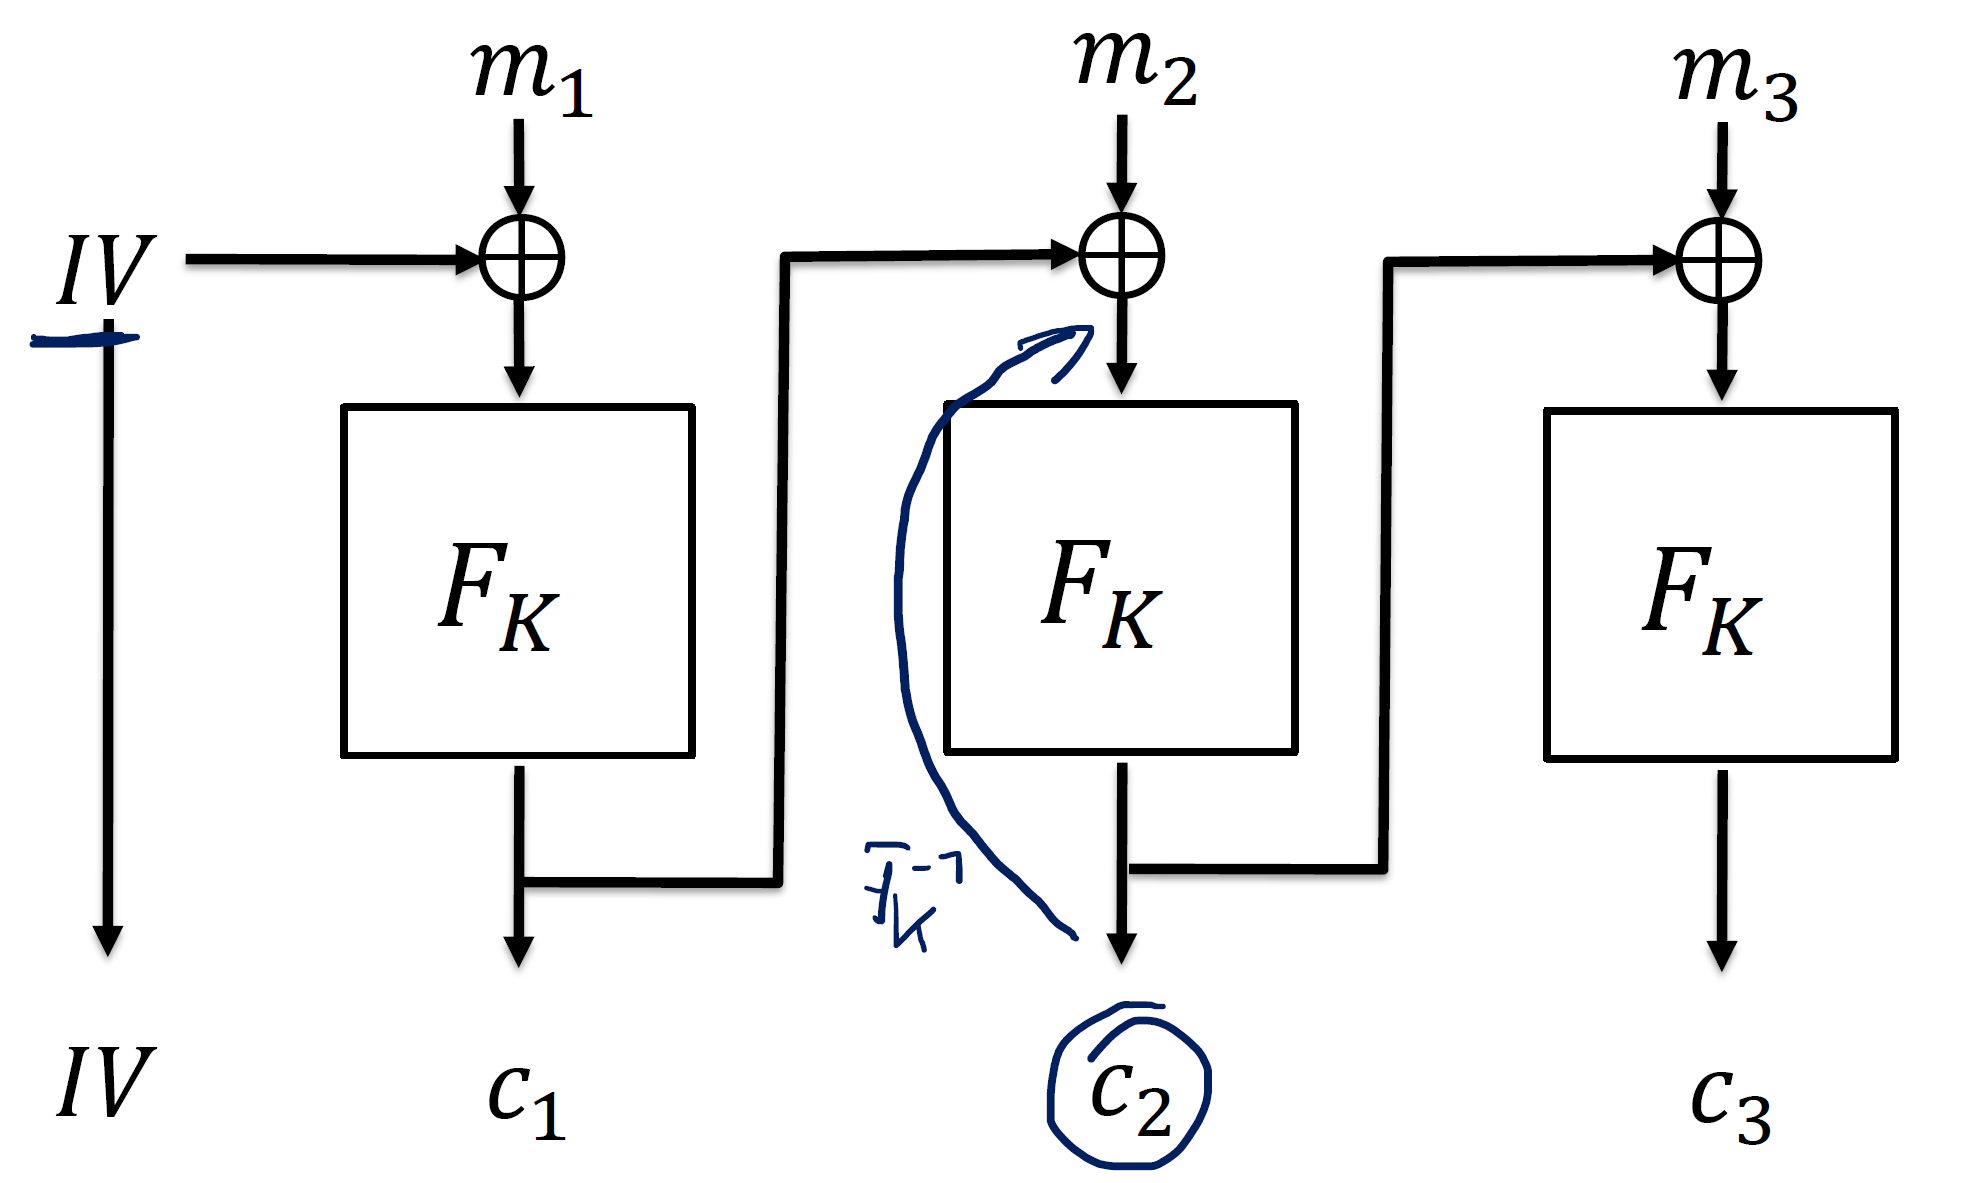
\includegraphics[width=120mm]{Graphics/Block Ciphers/bc9.png}
		\end{center}
		\begin{itemize}
			\item IND CPA secure for uniformly random IV if 𝐹is PRP
			\item Encryption must be performed sequentially
			\item Decryption is local
		\end{itemize}
	
	\subsection{Chained CBC Mode}
		\begin{center}
			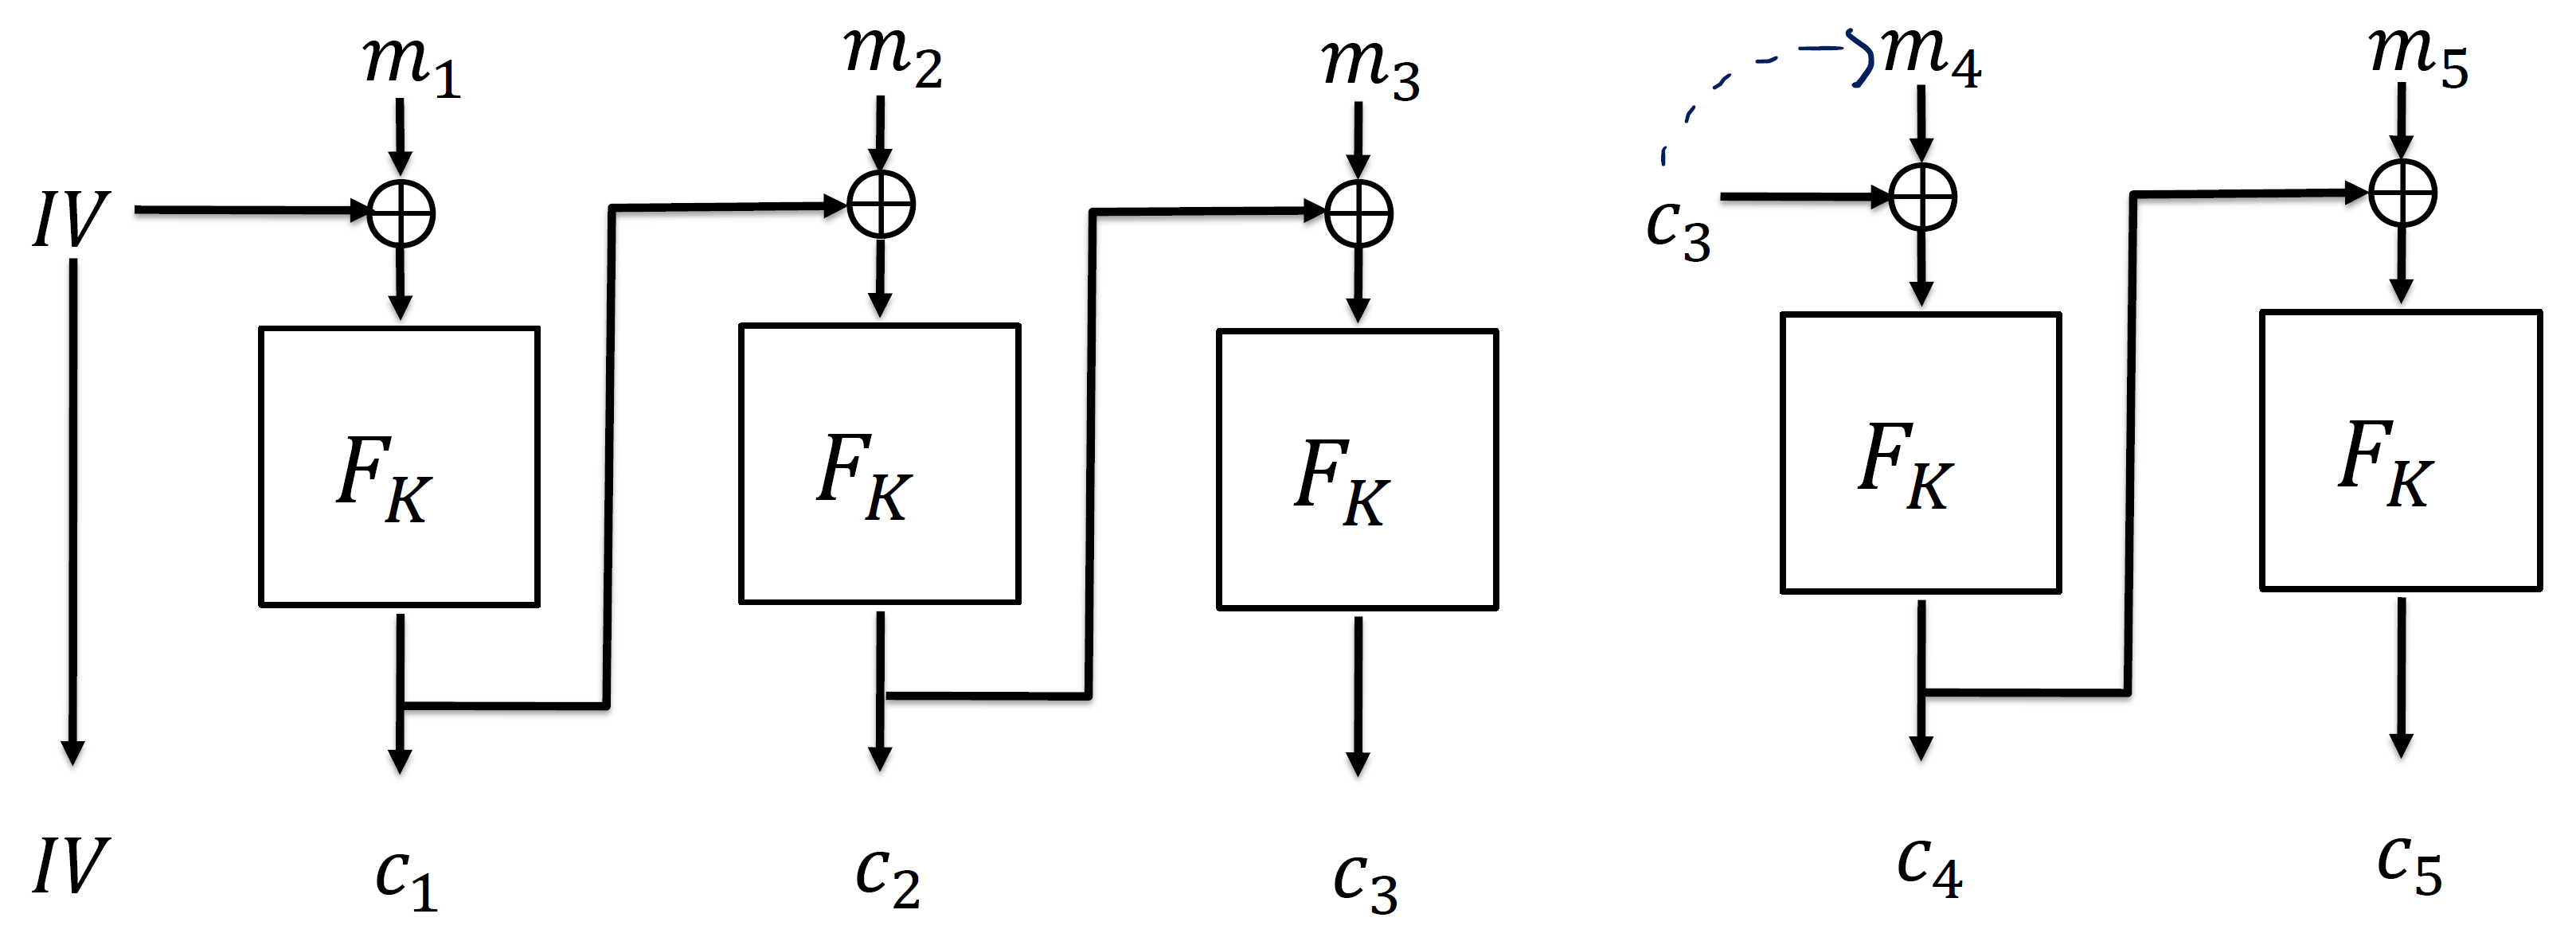
\includegraphics[width=120mm]{Graphics/Block Ciphers/bc10.png}
		\end{center}
		\begin{itemize}
			\item \textbf{Not} IND-CPA secure!
		\end{itemize}
	
	\subsection{Output Feedback (OFB) Mode}
		\begin{center}
			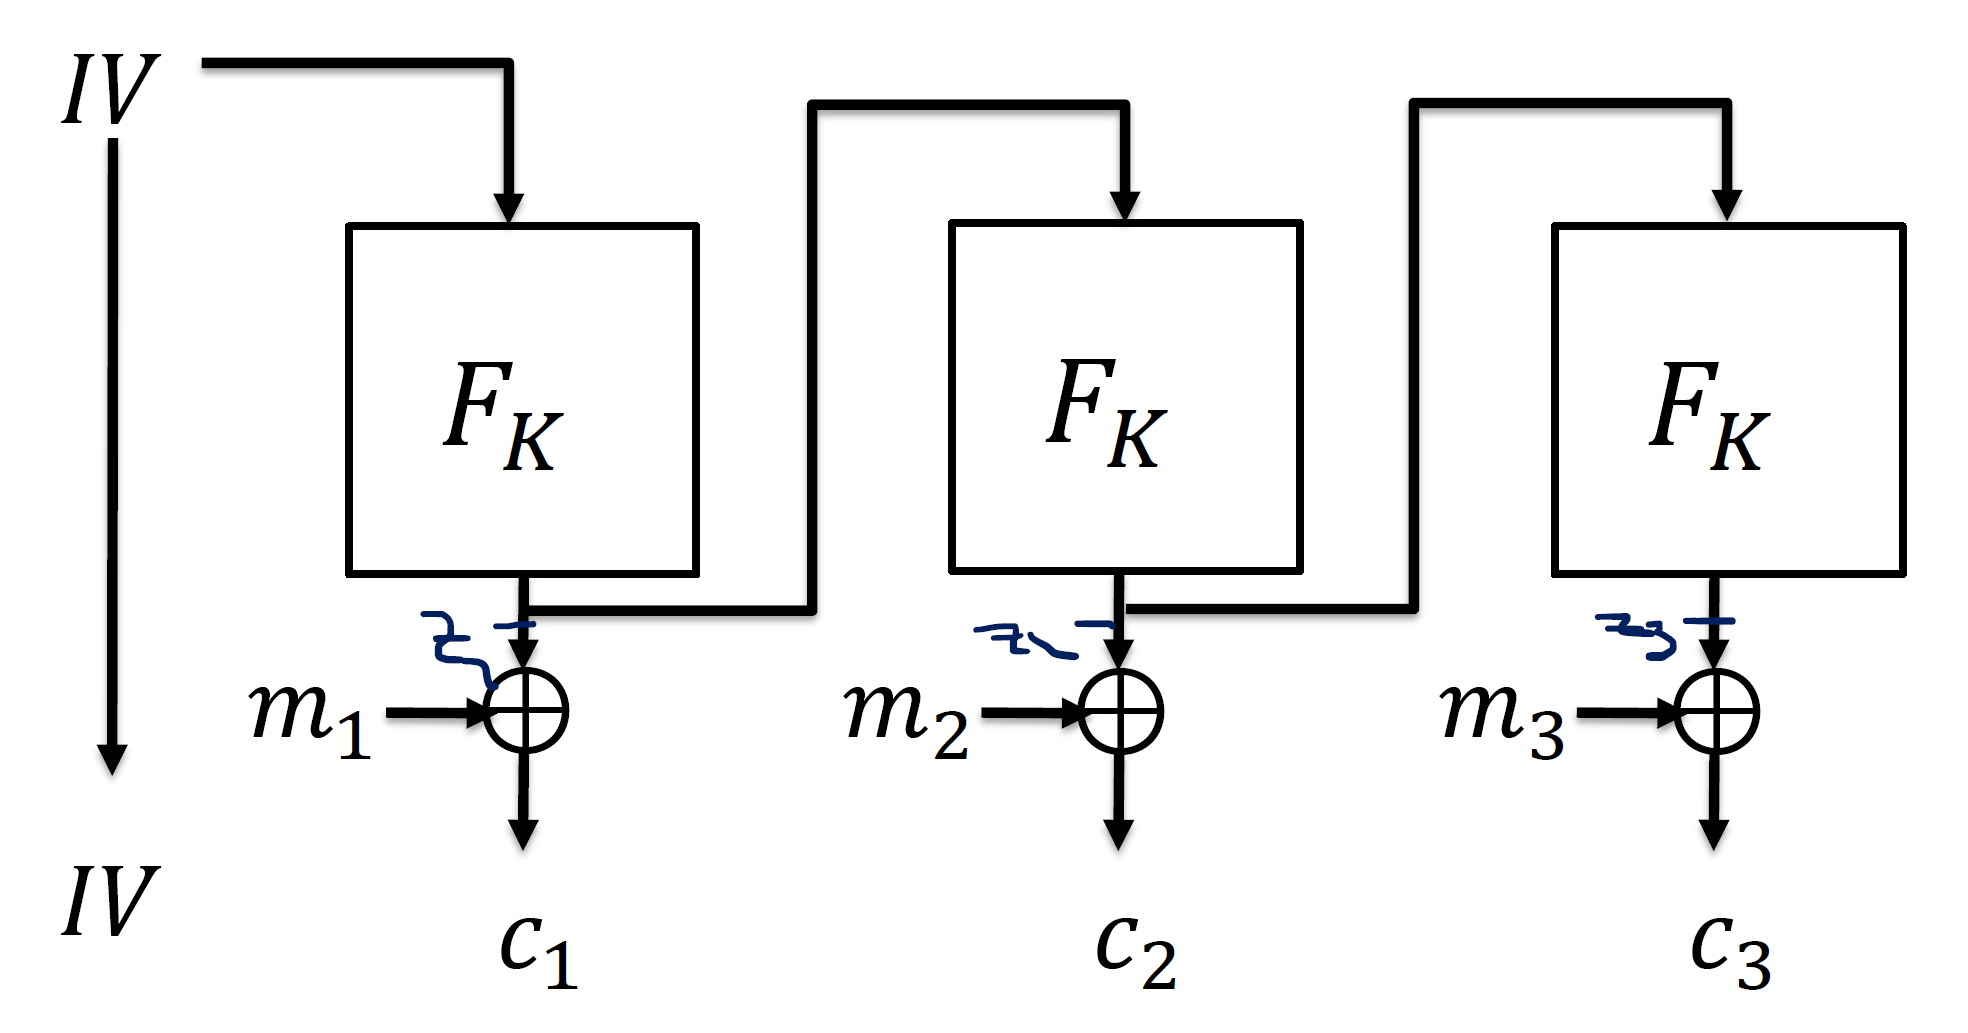
\includegraphics[width=120mm]{Graphics/Block Ciphers/bc11.png}
		\end{center}
		\begin{itemize}
			\item IND-CPA secure for uniformly random IV if $F$ is PRF
			\item Encryption and Decryption must be performed sequentially!
			\item Pad can be precomputed
		\end{itemize}
	
	\subsection{Counter (CTR) Mode}
		\begin{center}
			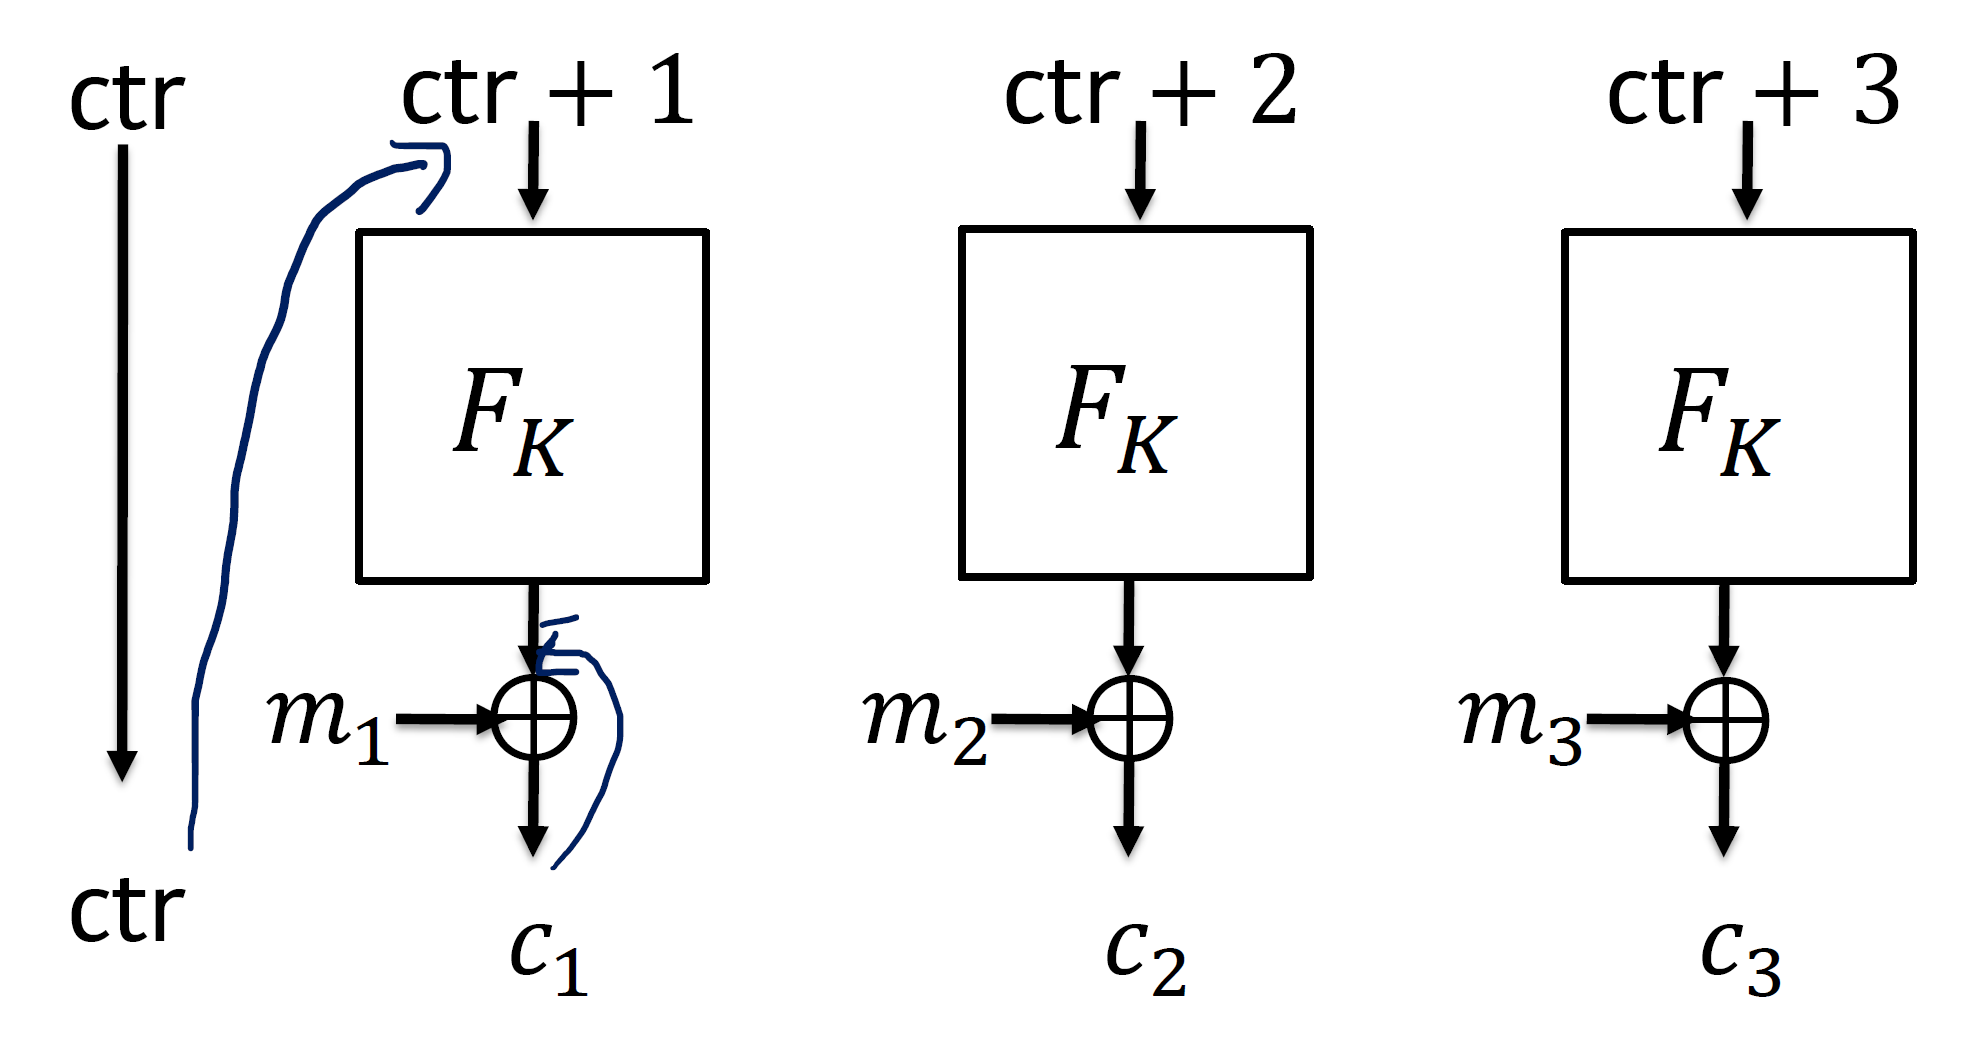
\includegraphics[width=120mm]{Graphics/Block Ciphers/bc12.png}
		\end{center}
		\begin{itemize}
			\item IND-CPA secure for uniformly random ctr if $F$ is PRF
			\item Encryption and Decryption are local/can be parallelized/precomputed
			\item Not reason not to use this one!
		\end{itemize}

\section{Summary}
	\begin{itemize}
		\item Blockcipher modes of operation provide a way to encrypt long messages
		\item ECM provides very little security $\rightarrow$ should only be used in very special scenarios
		\item CBC is ok!
		\item Chained CBC is not ok!
		\item OFM is ok!
		\item Use CTR whenever possible!
	\end{itemize}


























\chapter{Cryptanalysis}

\section{Security goals viewed by Cryptanalysis}
	\begin{itemize}
		\item In general, security of crypto primitives can be hard to define
		\item « Extreme definitions » don’t work, exemple:
		\begin{itemize}
			\item Secret key should be impossible to find\\
			$\Rightarrow$ Too weak
			\item A Block cipher should behave in all respects like a random permutation\\
			$\Rightarrow$ Impossible to achieve
		\end{itemize}
		\item Security proofs need formal definition. Cryptanalysts don’t!
		\item Basically, any « non generic » property might become a weakness
		\begin{itemize}
			\item Some generic properties might also be weaknesses showing bad parameters
		\end{itemize}
	\end{itemize}
	A first remark is that security notions are not intuitive in the field of cryptology. 
	Even the meaning of the word « attack » is relative and shifts with time or with respect to the point of view of the speaker. 
	In particular, the security notions involved in security proofs can be very different from the one we see in cryptanalysis. 
	For security proofs, a formal definition is required; for cryptanalysts, an attack scenario with a potential weakness that could be exploited is a better justification. 
	The choice of scenario has greatly evolved with time. 
	In the early days of historical crypto, ciphertext-only attacks were the reference.
	Nowadays, a wide range of interactive attacks are considered.\\
	For this reason, just asking for the secret-key to be impossible to recover by an attacker isn’t enough. 
	It might not prevent them from deciphering messages or from performing unauthorised modifications. 
	At the other extreme, some definitions can be too strong, simply because they are impossible to achieve. 
	We give an example in the next slide.\\
	The current consensus among secret-key cryptographers is that any explicit, non-generic, 
	property of a cryptographic primitive is a potential weakness (at least, as long as it can be made explicit with an efficient enough computation). 
	In some cases, generic weaknesses simply show that some desired primitive is just impossible to construct in a secure way.

\section{Block Ciphers}
	\begin{center}
		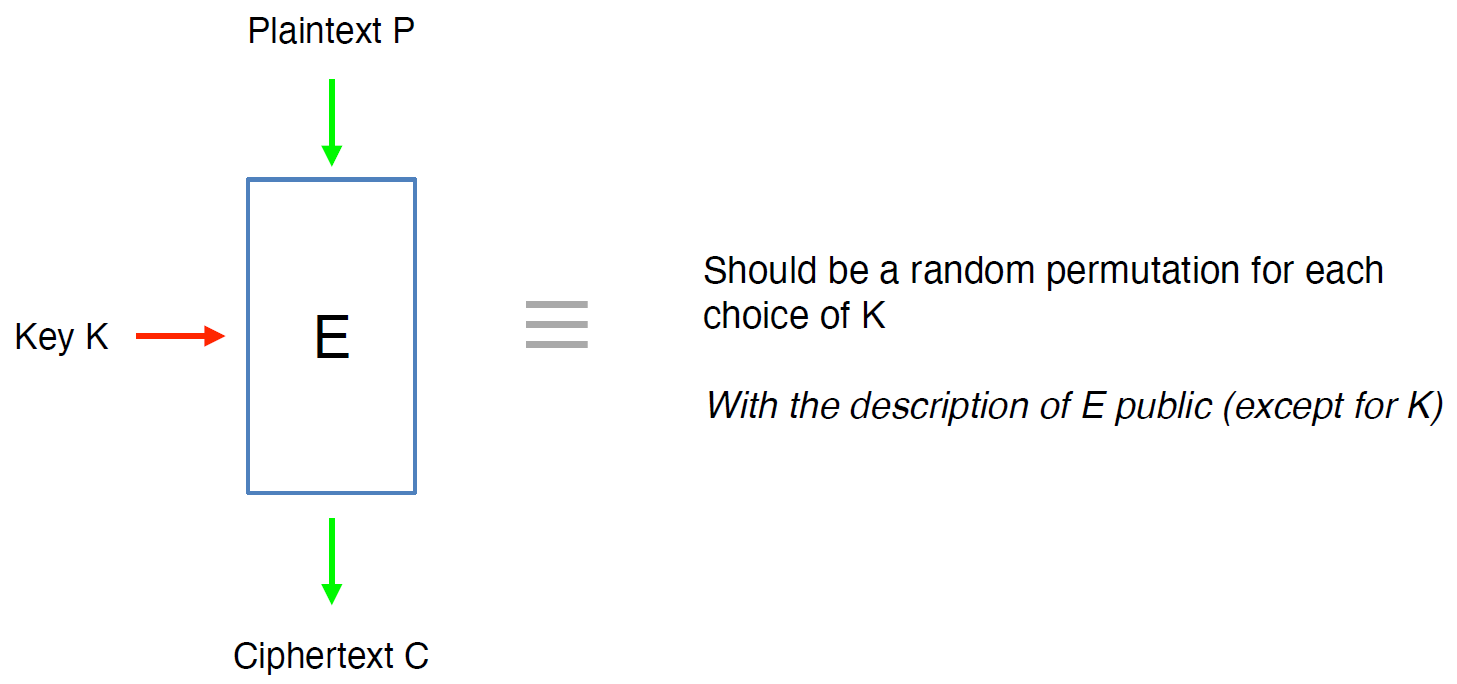
\includegraphics[width=140mm]{Graphics/Cryptanalysis/c1.png}
	\end{center}
	A first idea would be to request that a block cipher should behave like a random permutation in all respects for every choice of the key K. 
	Furthermore, following Kerckoffs’ principle, we still want this to be true when the description of the cipher itself is public and only the key remains secret.
	\begin{itemize}
		\item This informal definition is impossible to achieve
		\begin{itemize}
			\item Indeed, a random permutation doesn’t generally have a compact description
		\end{itemize}
		\item Generic attacks
		\begin{itemize}
			\item Exhaustive key search
			\item Plaintext block collisions are visible on Ciphertext block
		\end{itemize}
		\item[$\Rightarrow$] Key size and block size should be large enough. Today’s standard:
		\begin{itemize}
			\item At least 128 bits for key size, 192 or 256 are better when possible
			\item At least 128 bits for block size\\
			(64 bits still appears in legacy applications)
		\end{itemize}
	\end{itemize}
	Unfortunately, this definition cannot be achieved. 
	Indeed, by construction the block cipher has a compact description (in the form of its program), which is impossible for a truly random permutation.\\
	Instead, for security proofs, one turns to the notion of random permutation family which we will not revisit during this lecture.\\
	Since a block cipher is a permutation acting on plaintext-block values and chosen in a large but finite family by instantiating the key, some generic attacks arise. 
	First, since there are only finitely many keys, an attacker could (in principle) try all of them to recover the correct one. 
	Due to Shannon’s information theory, even a few blocks of data are enough to uniquely characterise the correct key. 
	To make this attack infeasible, cryptographers use extremely large sets of possible keys. 
	The current choice of key size is between 128 and 256 bits. 
	As a consequence, exhaustive search is infeasible even for attackers possessing tremendous computing powers and willing to use them for years or even decades.\\
	Another generic property is that encrypting the same block of plaintext twice yields the same ciphertext. 
	This can lead to devastating attacks. 
	As a consequence, block-ciphers always need to be used in a way that prevents such collisions between plaintext values from occurring. 
	This is taken into account when constructing « modes of operation », which are basically recipes for using block ciphers. 
	Furthermore, the block size should be large enough to prevent collisions from appearing when blocks are randomly chosen. 
	For this reason, modern block ciphers operate on 128 bits at a time.

\newpage
\section{DES}
	\subsection{DES: an outdated but interesting example}
		\begin{itemize}
			\item DES = Data Encryption Standard
			\item Block Cipher developed in the 70s at IBM
			\item NIST standard from 1976 to 2005
			\item DES is a Feistel cipher with a 56-bit key and 64-bit blocks
			\item Even in 1976, the key size was on the low side
		\end{itemize}
		During this lecture, we are going to use DES as an example to present some cryptanalytic results. 
		Despite being outdated, this algorithm has motivated a lot of research in cryptanalysis and led to several seminal breakthroughs. 
		In addition, since it was a NIST standard from 1976 to 2005, it is still often encountered in legacy applications. 
		This cipher has 56-bit keys and 64-bit blocks. 
		Note that even when it is was introduced, its key size was already considered too small by many people in academia.
	
	\subsection{How to have longer keys?}
		\begin{itemize}
			\item Modify the algorithm to change key size
			\begin{itemize}
				\item In the long run, it led to AES (Advanced Encryption Standard)
				\item In the early days, FEAL tried to improve on DES
			\end{itemize}
			\item Incorporate the algorithm in a bigger structure:
			\begin{itemize}
				\item Multiple DES (Introduced by Diffie-Hellman 77)
				\item DES-X (Rivest’84, unpublished)
			\end{itemize}
		\end{itemize}
		Because of DES small key size, the question of increasing the key size quickly arose. 
		One obvious avenue is to redesign a new cipher with bigger keys. 
		However, the crypto community soon discovered that this is harder than it seems and many attempts were broken which helped slowly building cryptanalytic expertise within academia.
		Eventually, NIST even became confident that this expertise was very strong and asked the community to design the successor of DES in the open AES competition.\\
		Another avenue is to assume that DES is well-designed, despite its small key, and to integrate it into a bigger construction to obtain larger keys.
	
	\subsection{Multiple DES - Diffie-Hellman 77}
		Another way to obtain a variable length key would be to use the currently proposed standard, but to encipher $m$ times with $m$ independent 56-bit keys.
		This would hopefully yield a 56$m$-bit key, but additional analysis is required.
		For example, enciphering twice with two monoalphabetic ciphers is equivalent to enciphering only once with a third monoalphabetic cipher.
		If cipher one carries $A$ to $F$ and cipher two carries $F$ to $C$, then the overall effect is to carry $A$ to $C$.
		This is because monoalphabetic ciphers form a semi-group under composition.
		It is highly doubtful that the proposed standard possesses this property.\\
		
		A first method, proposed by Diffie and Hellman in 1977 is simply to encrypt several times with independent keys. 
		They remarked that if DES was hiding a group-like structure, this approach would be doomed. 
		It took some time for the community to rule out this possibility.

\newpage
	\subsection{Double DES - Diffie-Hellman 77}
		After introducing multiple DES, they show that m=2 isn’t secure
		\begin{center}
			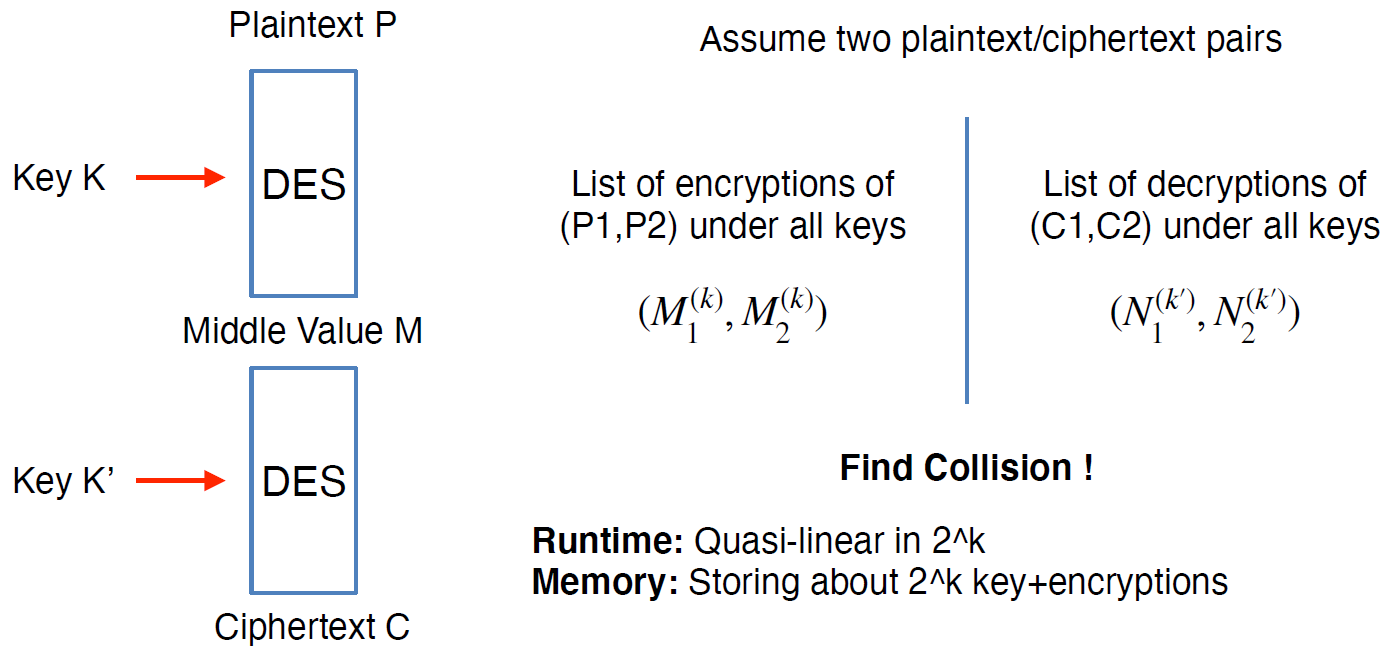
\includegraphics[width=140mm]{Graphics/Cryptanalysis/c2.png}
		\end{center}
		In the same paper, Diffie and Hellman show that encrypting twice isn’t good enough and doesn’t provide the security level that one should expect from 112-bit keys. 
		To see that, assume that we know the encryption of two plaintext blocks. 
		Indeed, one isn’t enough to characterise the key of double DES.
		Remark that if we encrypt the plaintext with the first half of the key and decrypt the ciphertext with the second half, we obtain the same middle values. 
		Moreover, for wrong keys, this event is really unlikely.\\
		
		As a consequence, we construct two lists, the first with all encryptions under all first half-keys and the second with all decryptions. 
		We expect very few collisions between these lists and every collision give a candidate key. 
		The right key is, of course, within this small set and it is easy to test it (for example by decrypting some extra text). 
		This works because collisions can be found efficiently.


\section{Finding Collisions in a list or between lists}
	\begin{itemize}
	    \item This is a major algorithmic tool in cryptanalysis
	    \item Can be done in quasi-linear time in the lists’ sizes\\
	    \item Basic idea for a single list:
	    \begin{itemize}
	        \item Sort the list of size $N$ (takes $O(N \cdot log(N))$ comparisons)
	        \item Read it in order. Collisions will be between consecutive elements!
	        \item Any ordering of the elements work (a natural ordering isn’t needed)\\
	    \end{itemize}
	    \item With two lists:
	    \begin{itemize}
	        \item Sort both
	        \item Start at the beginning of both lists, compare elements, advance the smallest
	        \item Iterate until a collision is found
	    \end{itemize}
	\end{itemize}
	\begin{center}
	    Extra care needed to get \textbf{all} collisions
	\end{center}
	In fact, searching for collisions within two lists or inside of a single list is a very important tool in cryptanalysis. 
	We will use it many times throughout the crypto course.\\
	The simplest idea is to test all pairs. However, this yields an algorithm whose time is quadratic in the lists sizes. 
	In the double DES example, with two lists containing $2^{56}$ elements, we would have to try $2^{112}$ pairs. 
	As a consequence, this wouldn’t be an improvement on exhaustive search at all.\\
	To outperform this, the basic idea is to start by sorting the list (or lists). 
	Thanks to fast algorithms like quicksort, this can be done in quasi-linear time. 
	After sorting, equal elements become neighbours in a single list. 
	So to discover them, it suffices to read the sorted list in order.\\
	With two lists, reading out the collisions is slightly more difficult. 
	The idea is to start by pointing to the first elements of the two lists and compare them. 
	Then advance the pointer corresponding to the smallest element to the next element in the same list. Compare again and repeat.\\
	Note that if there are many collisions and we want to find all of them, we need to take extra care. 
	Typically, if after sorting a single list we have ten consecutive elements which are equal, we have to build all pairs of elements among the ten and to construct 45 collisions. 
	In many applications like double DES for example, this is usually not needed.
	
\section{Triple DES - NIST standard (deprecated, disallowed after 2023)}
	\begin{center}
		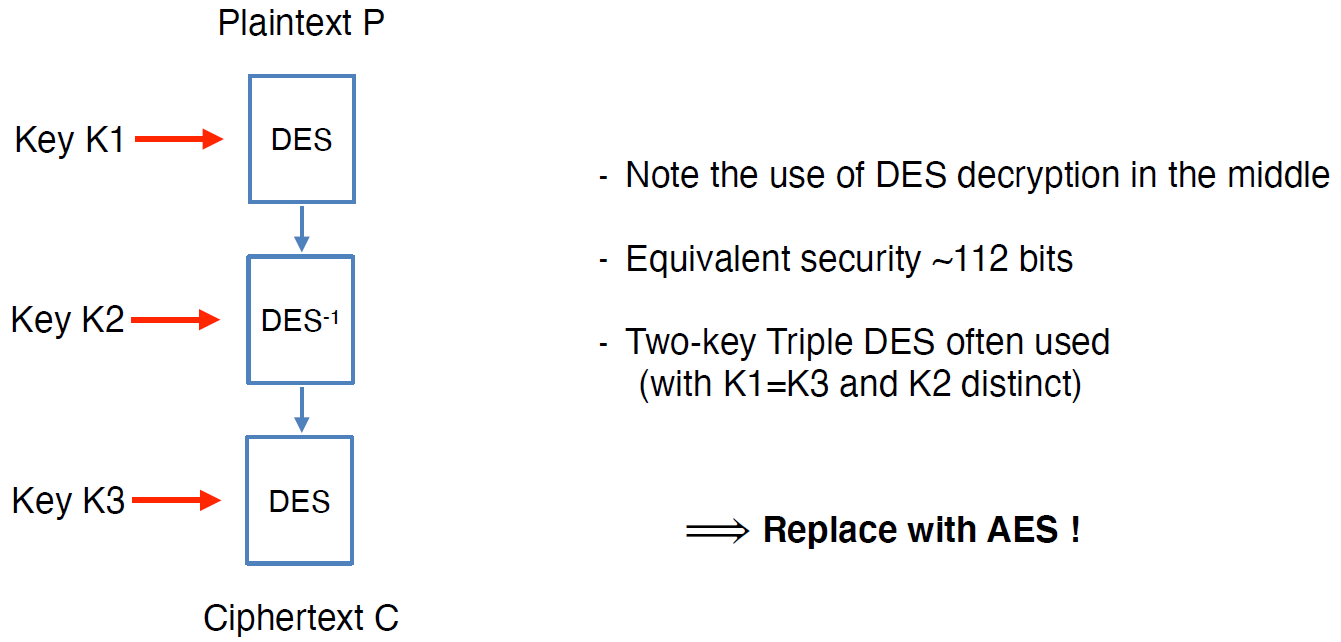
\includegraphics[width=140mm]{Graphics/Cryptanalysis/c3.png}
	\end{center}
	Because of the meet-in-the-middle attack on double DES, it turns out that to really get more security using multiple DES, we need to use triple DES. 
	In fact, triple DES still exists as a NIST standard, but will be disallowed after 2023. 
	Of course, we can still use this attack on triple DES to reduce its security to 112 bits (even if the overall key size is 168 bits). 
	Note that the attack now construct unbalanced lists, one of size $2^{56}$ (corresponding to the first key) and the other of size $2^{112}$ (corresponding to the last two keys). 
	Because of these unbalanced sizes, it is worth noting that there is a way to do the collision search that only requires a memory of the order of $2^{56}$ blocks. 
	Indeed, once the first list is constructed and sorted, we can build the second list one element at a time and use a dichotomy search to look for each element in the first list.\\
	Because the security can’t achieve 168 bits, the standard contains what is called two-keys triple DES, where the first and last keys are set to be identical. 
	Note that in the standard the middle invocation of DES decrypts with the second key rather than encrypt.
	It can be seen as a weakness. 
	For example, with two-key triple DES, if the first two keys are equal, the overall construction degenerates to simple DES. 
	In fact, this was done on purpose by NIST, to allow triple-DES equipment to perform simple DES by using this degenerate keys.\\
	You might still encounter triple DES in legacy applications, but it should be replaced by AES.

\section{Linear and Differential Cryptanalysis}
	\begin{itemize}
		\item The effort on studying DES (and other block ciphers like FEAL) led to:
		\begin{itemize}
			\item Differential Cryptanalysis (Biham/Shamir 1990)
			\item Linear Cryptanalysis (Matsui/Yamagishi 1992, Matsui 1993)\\
		\end{itemize}
		\item Both techniques consider probabilistic properties of the encryption:
		\begin{itemize}
			\item Found by examining building blocks
			\item Under the heuristic assumptions that events behave independently\\
		\end{itemize}
		\item These probabilistic techniques have been extended to other attacks
		\begin{itemize}
			\item Linear and differential remain essential for evaluating ciphers
		\end{itemize}
	\end{itemize}
	Two of the most fruitful methods that appeared by studying DES and some of the other block ciphers it inspired are the differential and the linear cryptanalysis techniques. 
	The first was invented by Biham and Shamir in 1990, the second two years later by Matsui and Yamagishi.\\
	These techniques share an important feature. 
	Indeed, both of them rely on observing probabilistic relations that are satisfied in the target block cipher more often than they would be in a random permutation. 
	Because of the large block sizes (and key sizes), such relations cannot be predicted by a brute force method. 
	Instead, they are first constructed on small building blocks of the cipher and then composed into a property of the block cipher (or of a reduced version of the cipher for some attacks).
	The composition techniques that are used are usually heuristic and rely on the assumption that successive rounds behave independently.\\
	They are many more recent attacks that share a lot of these features. 
	To name a few, we can cite the square attack, the boomerang attack or the impossible differential attack. 
	However, the linear and differential attacks remain essential to evaluate block ciphers and it is important to have some basic knowledge about them.

\section{Differential Cryptanalysis}
	\subsection{Fundamentals}
		\begin{center}
			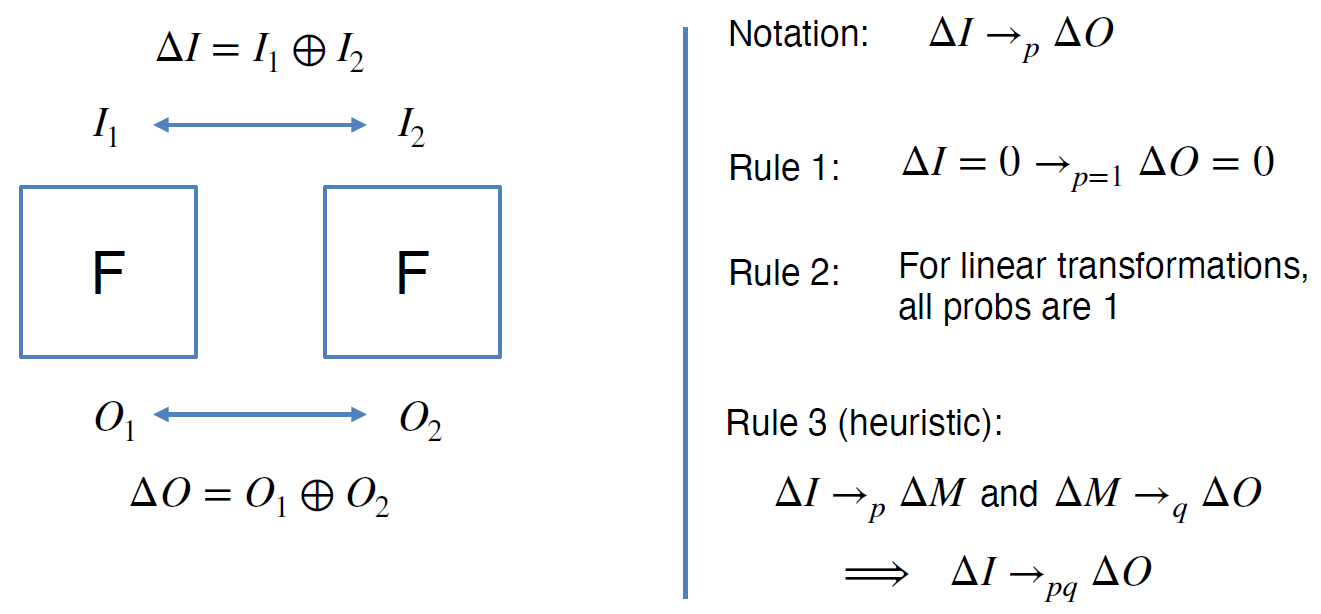
\includegraphics[width=140mm]{Graphics/Cryptanalysis/c4.png}
		\end{center}
		In the differential attack, we look at pairs of blocks, $I_1$ and $I_2$, that are encrypted into outputs $O_1$ and $O_2$. 
		The name differential comes from the fact that we study the relation between the difference of the inputs and the difference of the outputs. 
		Remember that, in our context, every block is formed of bit strings. 
		As a consequence, it is quite natural to study a bit-by-bit difference. 
		Moreover, when working with bits, operations modulo 2 are the most common choice. 
		Because of that, the difference of blocks is simply their Exclusive-OR.\\
		More precisely, for every possible input difference $\Delta I$, we count how many times it leads to an output difference, $\Delta O$. 
		After dividing by the number of possible pairs, we obtain the probability that $\Delta I$ leads to $\Delta O$. 
		We use the Notation at the top of the right column to indicate that $\Delta I$ leads to $\Delta O$ with probability $p$. 
		These probabilistic arrows are usually called differential characteristics.\\
		For example, for any block cipher (or any component of a block cipher), a zero difference in input always produce a zero difference in the output. 
		Similarly, for a linear transformation (on bits), the output difference is always the transformation by the linear map of the input difference.\\
		To be able to construct differential characteristics on a block cipher with many rounds, we need a way to compose probabilistic arrows. 
		For this, we use the third heuristic rule that says that we can combine two arrows where the output difference of the first is equal to the input difference of the second. 
		Moreover, the probability of the composition is the product of the individual probabilities, under the heuristic independence assumption.
	
	\subsection{Small example}
		Consider the ADD function with 2 input bits and 2 output bits:
		\begin{center}
			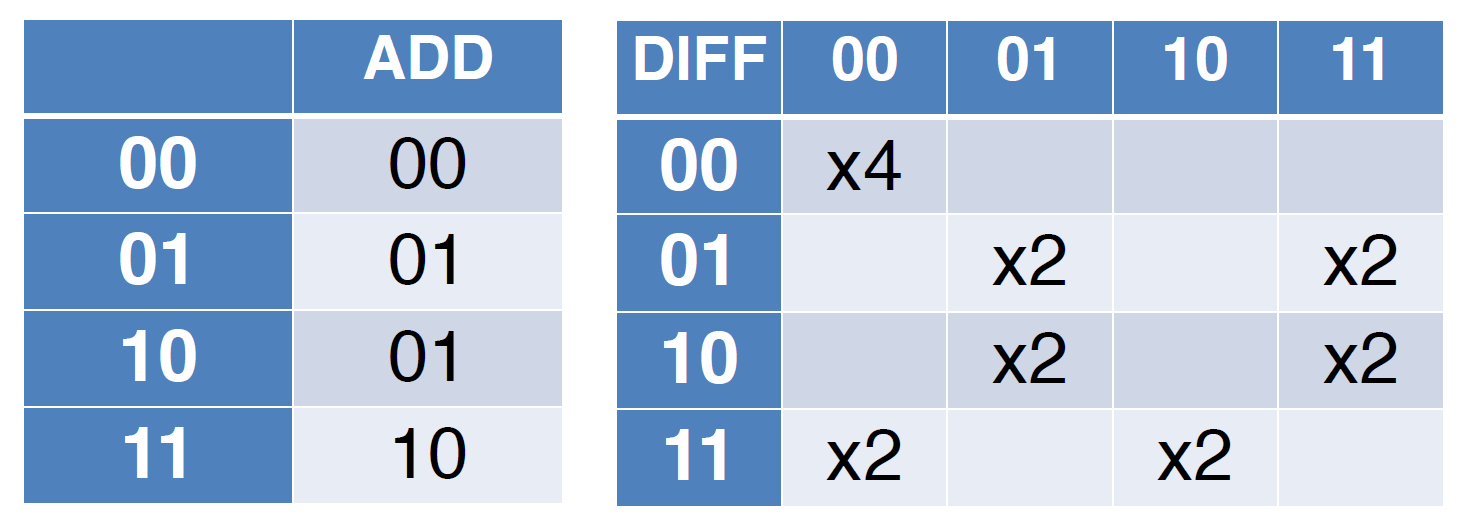
\includegraphics[width=140mm]{Graphics/Cryptanalysis/c5.png}
		\end{center}
		On this small example, we show a full table of differential counts for a function with two bits of input and two bits of output. 
		The chosen function is the addition of the two input bits, written in binary.\\
		The table on the right tells how many times each output difference appears for a given input difference and empty cells indicate that the corresponding output difference is not possible.
		
	\subsection{Principle of the attack}
		\begin{itemize}
		    \item Assume we have $\Delta I \to_p \Delta O$ for a block cipher (with $p >> 2^{-n}$)
		    \begin{itemize}
		        \item Encrypt many pairs with input difference
		        \item For the studied cipher $\Delta O$ is observed with probability close to $p$
		        \item For a random permutation $\Delta O$ is observed with probability close to $2^{-n}$\\
		    \end{itemize}
		    \item This yields a chosen plaintext distinguisher from a random permutation!\\
		    \item For key recovery, use the distinguisher on a restricted num of rounds
		    \item Together with exhaustive key search on (part of) the removed rounds
		\end{itemize}
		Once a differential characteristic is known for the full block cipher, we can build a distinguishing attack. 
		Namely, we are given access to an encryption device and want to determine whether it implements the target block cipher (with an unknown key) or a random permutation. 
		We simply encrypt many pairs with the prescribed input difference and observe how often the corresponding output occurs. 
		For the block cipher, the proportion is close to the probability $p$. 
		By contrast, for a random permutation, it is close to $2^{-n}$.\\
		The attack can also be used for key recovery. 
		For this, we start from a characteristic on a reduced number of rounds and query plenty of pairs with the prescribed input difference. 
		Then, we perform exhaustive search for the last round key, decrypt the output for one round and observe the difference. 
		For the correct guess, the prescribed output will occur more frequently. 
		There are subtleties to implement the attack when the key for the last round is too large for exhaustive search. 
		Indeed, in that case, the cryptanalysis needs to find a way to implement the attack using exhaustive search on a reduced part of the key.\\
		The details of how this can be done can vary depending on the exact specification of the block cipher we are attacking.


\section{Linear Cryptanalysis}
	\subsection{Fundamentals}
		\begin{center}
			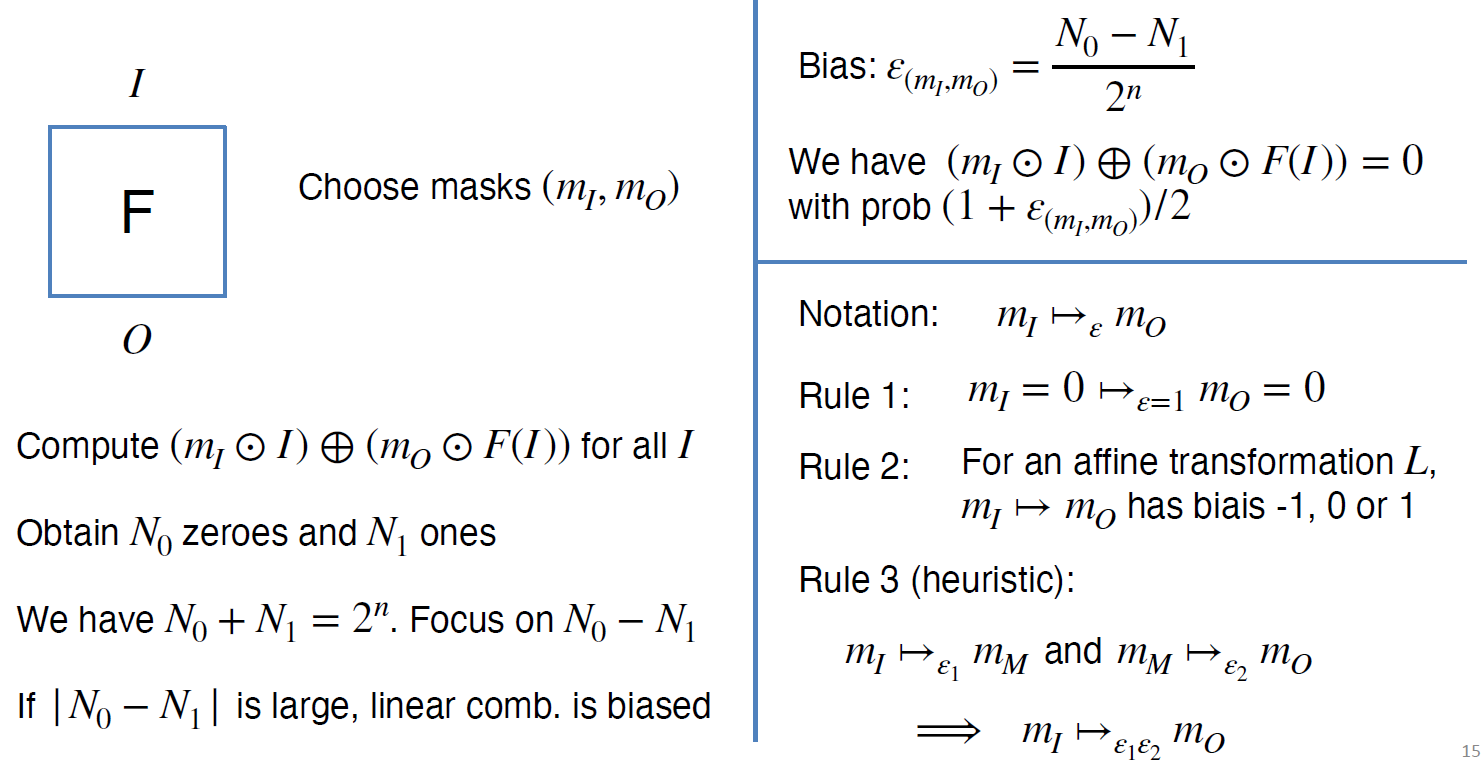
\includegraphics[width=140mm]{Graphics/Cryptanalysis/c6.png}
		\end{center}
		In linear cryptanalysis, we study the relation between inputs and outputs in a different way. 
		We choose two bit strings $m_I$ and $m_O$ (that we will call input and output mask) and, for input/output pairs $I-O$, 
		we study the distribution of the quantity ($m_I$ scalar $I$) XOR ($m_O$ scalar $O$). 
		In other words, we mask the input bits with the mask $m_I$ and the output bits with $m_O$, we count the number of '$1$' in the masked bit strings and compute the parity of this number, 
		namely we reduce the count modulo 2. 
		Over all inputs, let say that we observe a zero result $N_0$ times and a one result $N_1$ times. 
		Of course, $N_0 + N_1$ is equal to $2^n$, the total number of possible inputs. 
		Thus, the difference $N_0 - N_1$ encodes all the information we need about $N_0$ and $N_1$. 
		We now focus on this difference.\\
		When its absolute value is small, the result is balanced, that is zeroes and ones occur roughly as often as each other. 
		When it is large, there are much more zeroes or ones, depending on the sign of the difference.
		It is convenient to normalize the difference and consider the bias epsilon of $(m_I, m_O)$ which is defined as the difference divided by $2^n$. 
		Then, the probability to observe a zero is equal to (the bias +1) divided by two.
		Using a notation reminiscent of the one from differential cryptanalysis, we will write an arrow from $m_I$ to $m_O$ with the bias epsilon written as a subscript. 
		To avoid confusion, we use a different arrow in the notation.\\
		As before, there are some important rules that always hold. 
		First, for input and output masks equal to zero, we don’t observe any of the input bits or output bits. 
		As a consequence, the number of ones in this empty observation is always equal to zero and its parity is always zero. 
		Thus, the bias of this 0 to 0 arrow is equal to 1.\\
		For linear (and also affine) transformations, all arrows have bias equal to either 0, 1 or -1. 
		Showing this is a good exercise to become more familiar with the notion.\\
		The third rule is heuristic and consider a chain of two arrows, where the output mask of the first arrow is equal to the input mask of the second. 
		Then we have a composed arrow whose bias is the product of the biases of the initial ones.\\
		These rules can be used to construct linear characteristics for block ciphers built from many sub-components.
	
	\subsection{Small example}
		\begin{center}
			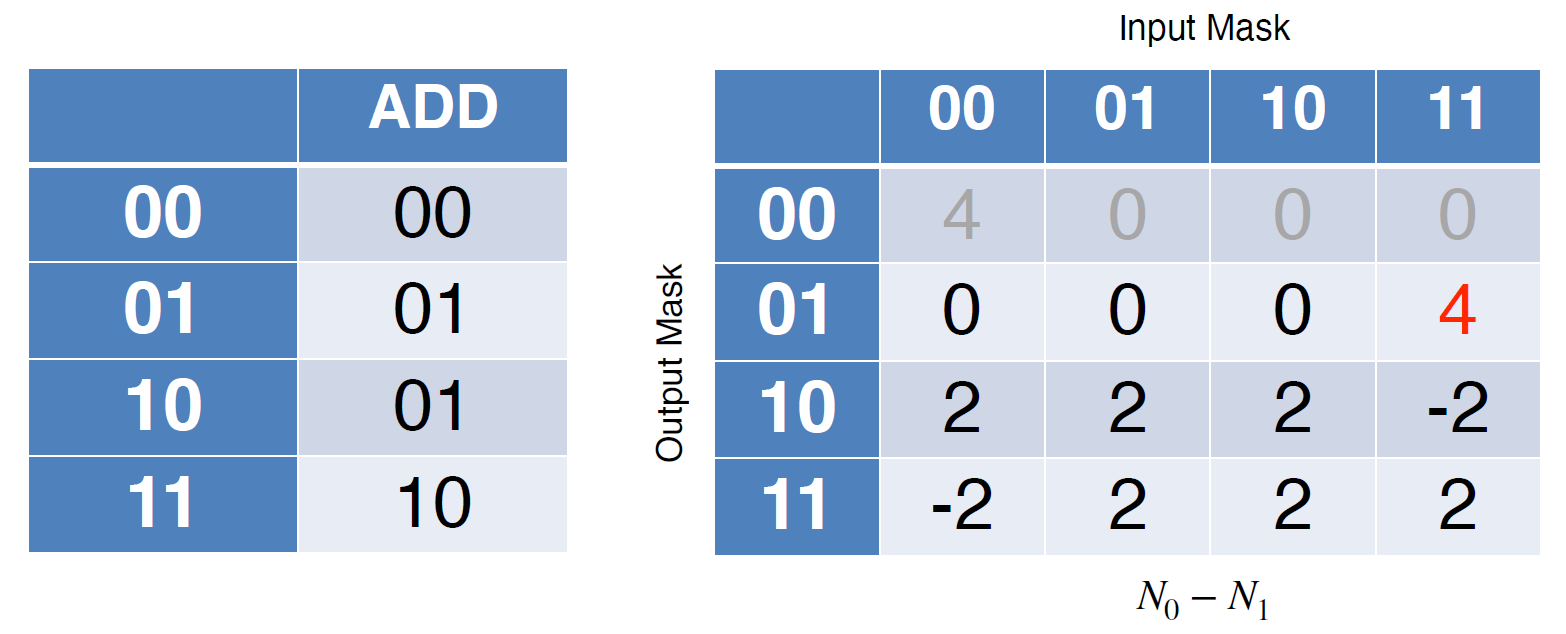
\includegraphics[width=140mm]{Graphics/Cryptanalysis/c7.png}
		\end{center}
		We now revisit our small example for linear cryptanalysis. 
		The first line is greyed out since the case of a zero output mask never provide any useful information because, in that case, we are not observing any of the output bits. 
		On the other hand, the first column where we do not observe the input bit can yield interesting information. 
		For exemple, the -2 at the bottom of the first column tells us that the XOR of the two output bits of an addition is more often equal to 1 than to 0. 
		The red 4 tells us that there is a linear relationship for input mask 11 and output mask 01.
		Indeed, the low order bit of a sum is equal to the XOR of the two input bits.

	\subsection{Principle of attack}
		\begin{itemize}
		    \item Assume we have $m_1 \mapsto_{\epsilon} m_0$ for a block cipher (with $\epsilon >> 2^{-n}$)
		    \begin{itemize}
		        \item Encrypt with inputs $I$ with output $O$, compute $(m_I \odot I) \oplus (m_O \odot O)$
		        \item For the studied cipher, large difference between num of zeroes and ones
		        \item For a random permutation, close to balance between zeroes and ones
		    \end{itemize}
		    \item This yields a known plaintext distinguisher from a random permutation!
		    \item For key recovery, we can take advantage of key mixed in using XORs
		\end{itemize}
		The principle of using linear cryptanalysis as a distinguisher is basically the same as the one we saw for differential cryptanalysis.\\
		However, for key recovery attacks, there is a very interesting twist. 
		This comes from the fact that in most block cipher, the key is incorporated by XOR it with intermediate values every now and then during the encryption process. 
		If we know a linear characteristic for a part of the cipher and want to XOR a key after this part, we can observe that this changes the value of the output scalar product 
		by a constant which is the parity of the number of ones in the corresponding key masked with the output mask. 
		This also composes well and as a consequence, the absolute value of bias of the global linear characteristic is unaffected by this specific way of introducing the key. 
		Only the sign will change (or not) depending on the value of one parity bit of the expanded key (coming from the key schedule).\\
		Of course, it is also possible to use the partial exhaustive search technique we described for differential cryptanalysis.

\section{Related Key attacks : Example of DES-X}
	\begin{center}
		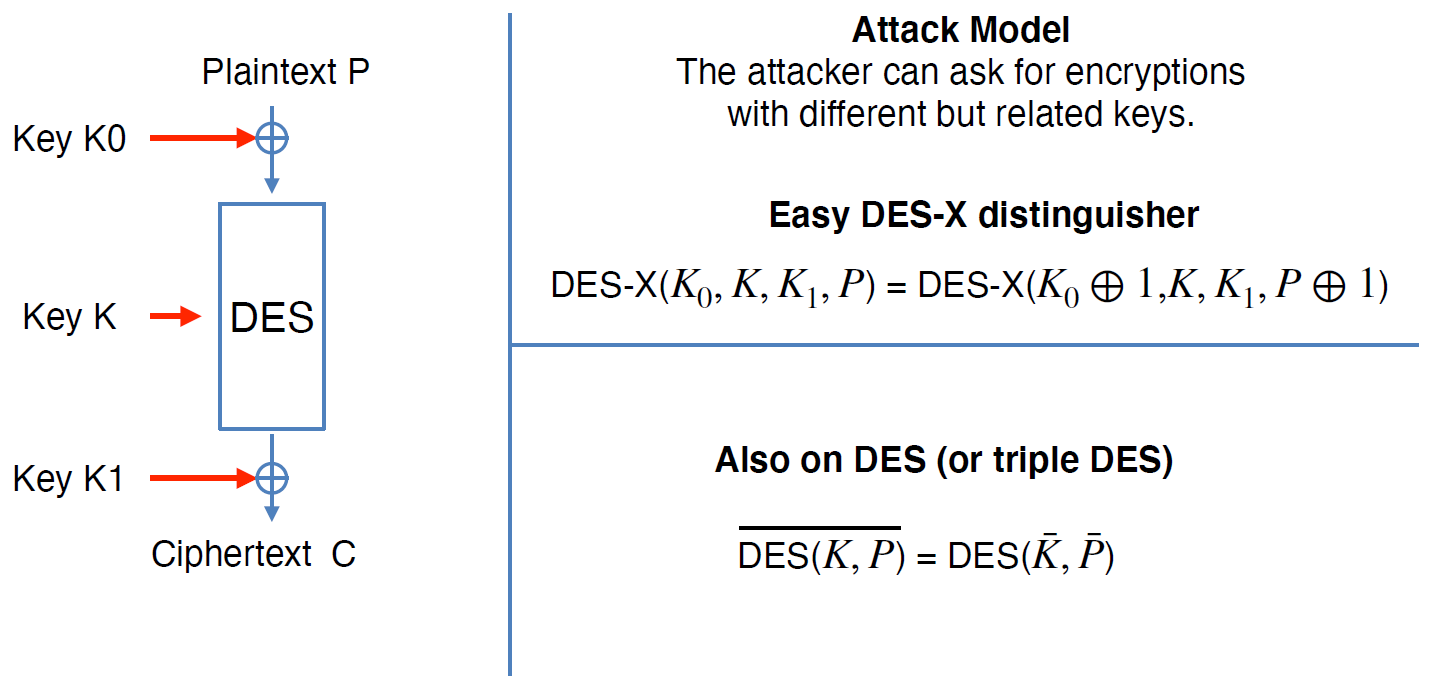
\includegraphics[width=140mm]{Graphics/Cryptanalysis/c8.png}
	\end{center}
	As a last example of block-cipher attacks, we now consider a new method called the related key attack. 
	It is a different attack model where the attacker can not only query the block cipher with its basic key but also with different but related keys obtained by XORing 
	the basic key with values which are arbitrarily chosen by the attacker. 
	It is also possible to replace XOR by another operation such as addition but care needs to be taken when defining the attack model.\\
	Related-key distinguishers arise naturally with some block ciphers. 
	A first example is the DES-X cipher proposed by Rivest to enlarge the key size of DES. 
	It consists in a sandwich structure where before and after DES encryption the plaintext and ciphertext blocks are XORed with two whitening keys K0 and K1.
	By itself it is an interesting technique that led to the Even-Mansour construction. 
	However, with DES-X, a related-key distinguisher can easily be built. 
	For example, it is clear that XORing any constant (let say 1) with both the plaintext block and the first whitening key while leaving everything else unchanged doesn’t change the ciphertext.\\
	Interestingly, there also is a simple related key distinguisher on DES itself. 
	Indeed, negating every bit of the plaintext and of the key at the same time creates a ciphertext which is the negation of the initial one.\\
	Related-key attacks may or may not be a problem in applications, it really depends on how the block-cipher is used. 
	However, block-cipher designers usually try to avoid them in order to prevent bad interactions in applications that could be vulnerable otherwise.

\section{Arbitrary related key attack model is too strong}
	\begin{center}
		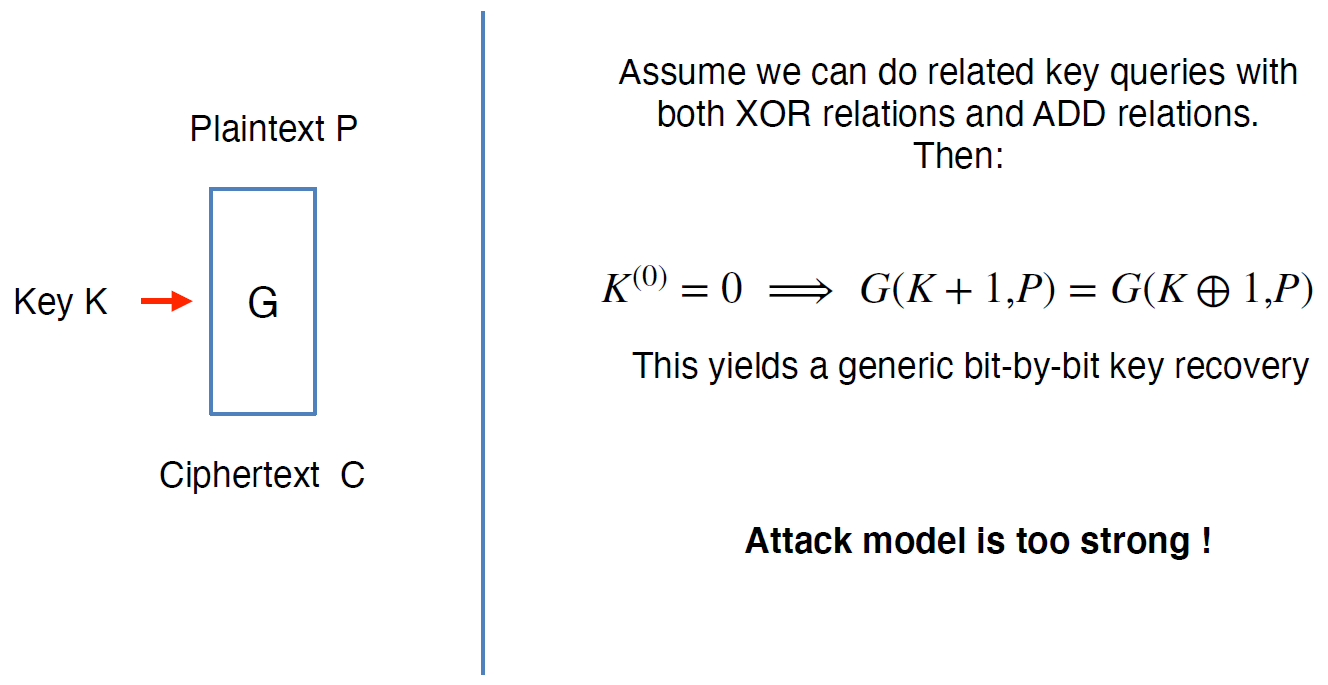
\includegraphics[width=140mm]{Graphics/Cryptanalysis/c9.png}
	\end{center}
	As mentioned in the previous slide, some care needs to be taken when considering related-key attacks. 
	Indeed, if the attacker is allowed to use arbitrary transforms of the initial key, there is an easy generic key recovery attack that becomes possible. 
	To show that assume that the adversary is allowed to either XOR the initial key with a constant of its choice or to ADD a chosen constant to the key (modulo $2^k$ where k is the key size).\\
	Remark that XORing the constant 1 to a key $K$ and adding 1 to the same key $K$ give the same result if and only if the lowest order bit of the key is a zero. 
	Moreover, testing if two keys are equal is easy to do by encrypting any plaintext block with both keys and comparing the resulting ciphertext blocks. 
	Thus, the adversary learns the first bit of the key. 
	By adding and XORing 2, 4, 8 and so on, he can also learn the remaining bits (with the exception of the top bit). 
	Of course, this exception is not a problem since once all the bits of the key except the last one are known, it suffices to test which of the two remaining possibilities is the correct key.\\
	As a consequence, when using related key attacks, one should always check that the model hasn’t been pushed in an extreme regime where this kind of generic attacks are possible.
































\chapter{Hash Functions}

\section{Fingerprinting}
	\begin{itemize}
	    \item Problem: You have a large file/object and want to compare to objects in a database
	    \item E.g. check if you object is in the database
	    \item Object too large to send to the server
	    \item $\Rightarrow$ Need a small unique identifier/digest of your object
	    \item \textbf{Hashing!}
	    \item Compress objects into a small fingerprint
	    \item $\Rightarrow$ Speed up comparisons/membership tests, smaller communication cost
	\end{itemize}


\begin{definition}[Hash Functions]\ \\
    \textbf{Syntax:}
    A family of hash functions is given by a pair of algorithms $(Gen,H)$
    \begin{itemize}
        \item $Gen(1^{\lambda})$: A probabilistic algorithm which on input $1^{\lambda}$ outputs a key $S$
        \item $H^S(x)$: A deterministic algorithm which on input a key $S$ and a string $x \in \{o,1\}^*$ outputs a hash value $h \in \{0,1\}^l$
    \end{itemize}
   	\begin{center}
		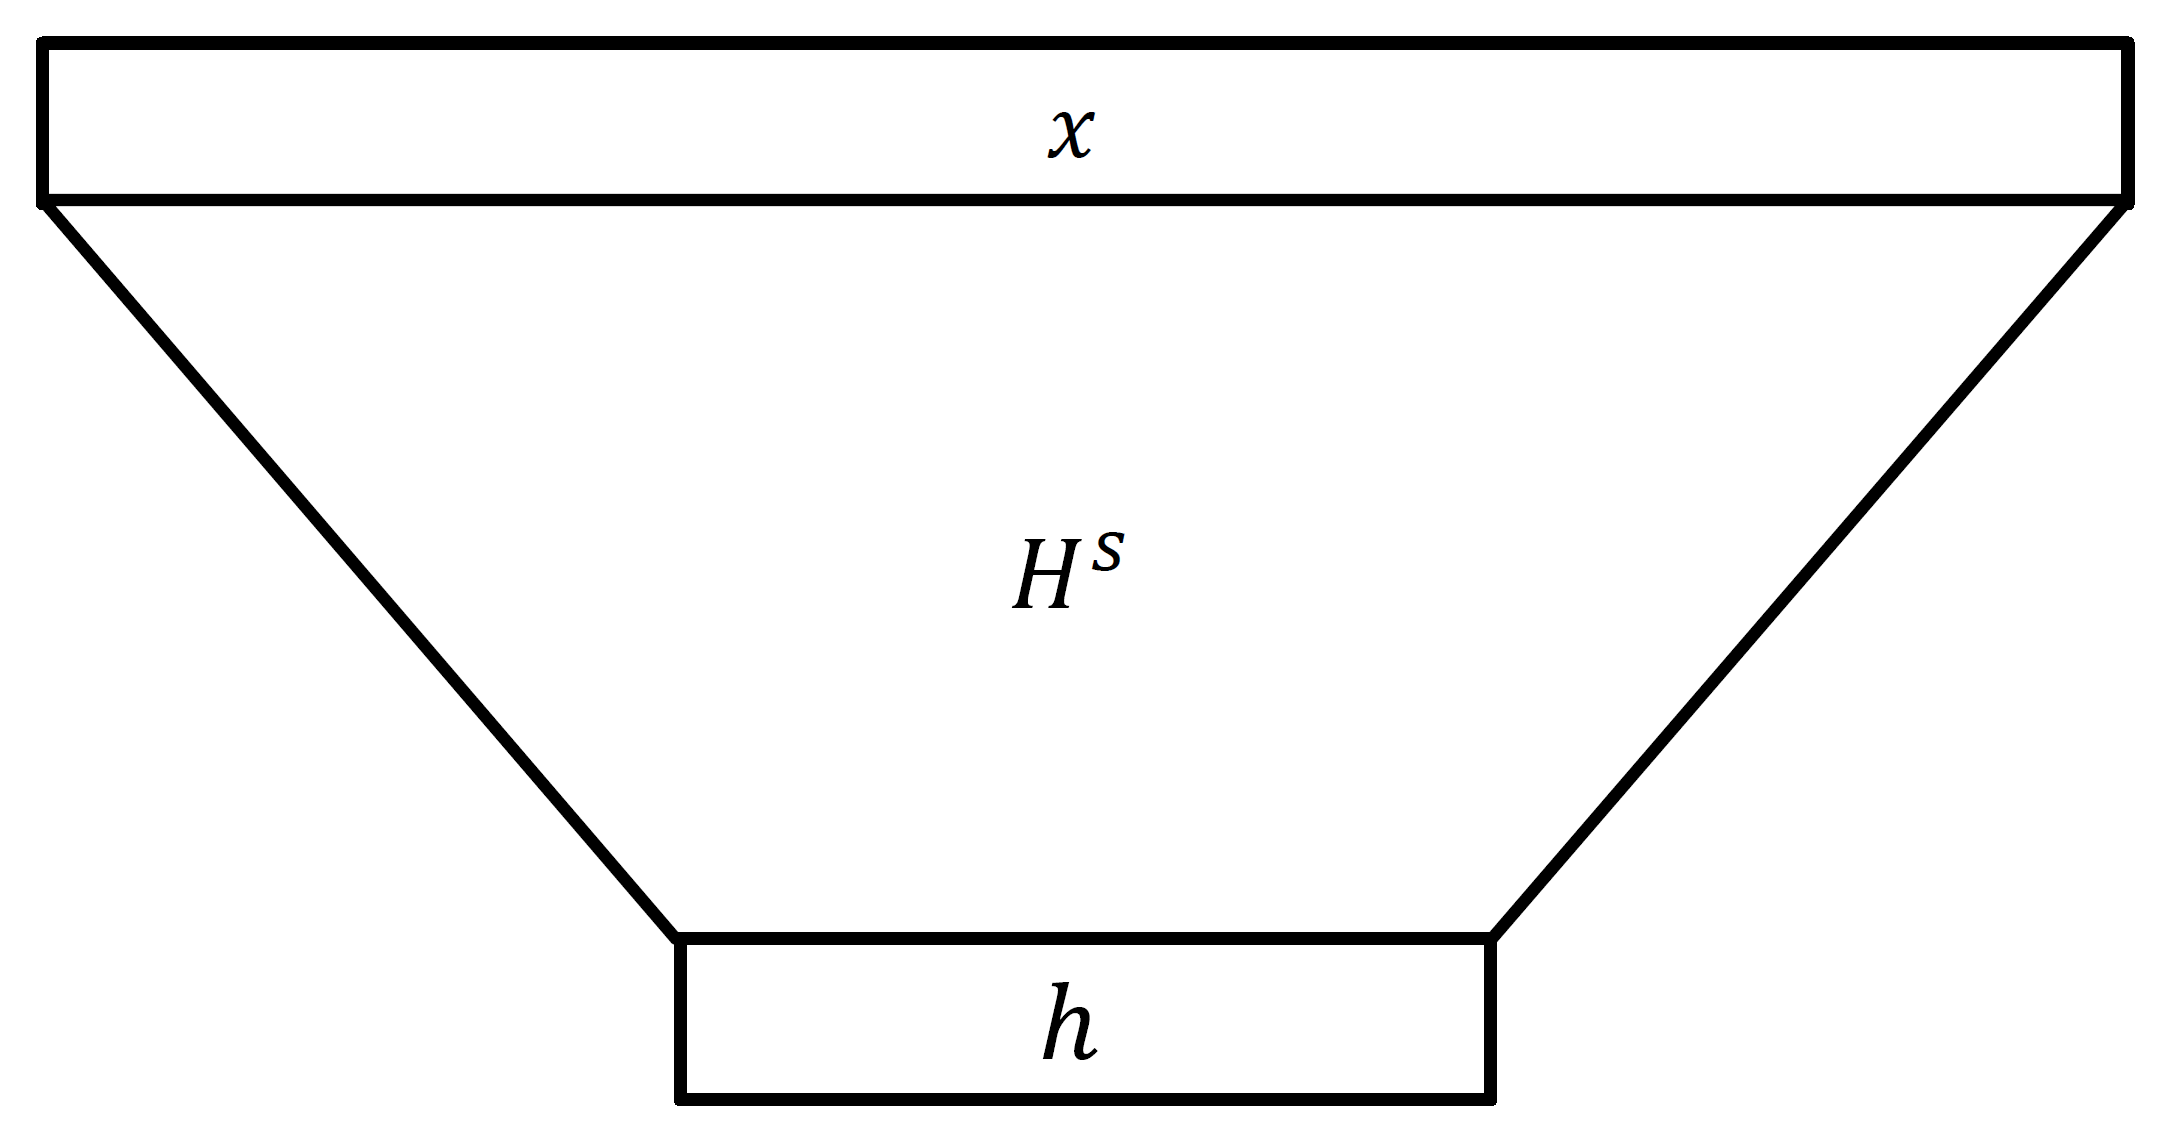
\includegraphics[width=120mm]{Graphics/Hash Functions/hf1.png}
	\end{center}
    \textbf{Remarks:}
    \begin{itemize}
        \item The output length $l=l(\lambda)$ only depends on $\lambda$
        \item If $H^S$ is only defined on inputs of length $l' > l$ we call $H$ a fixed-length hash function
        \item If we don't specify $Gen$ it just chooses uniformly random $s \leftarrow_{\$} \{0,1\}^{\lambda}$
    \end{itemize}
\end{definition}


\begin{definition}[Collision Resistance]
	Let $H: \{0,1\}^{l'} \to \{0,1\}^{l}$ with $l' > l$.\\
    A hash function $(Gen,H)$ is called collision-resistant, if for every PPT-bounded adversary $\mathcal{A}$ there exists a negligible function $v$ s.t. for all $\lambda \in \mathbb{N}$
    $$Pr[Hash-Col_{\mathcal{A}}(\lambda)=1] < v(\lambda)$$
   	\begin{center}
		\includegraphics[width=120mm]{Graphics/Hash Functions/hf2.png}
	\end{center}
\end{definition}

	\subsection{Examples}
		\begin{itemize}
			\item Assume $H$ is a collision resistant hash function
			\item Is $H'$ given by $H'^S(x) = H^S(x || 0^{\lambda})$ also collision resistant?
			\begin{itemize}
				\item Yes!
				\item Idea: Collision $x,x'$ for $H'$ yields collision $x || o^{\lambda}$, $x' || 0^{\lambda}$ for $H$
			\end{itemize}
			\item Is $H''$ given by $H''^S(x_1...x_n) = H^S(x_1...x_{n-1})$ collision resistant?
			\begin{itemize}
				\item No!
				\item $0...00$ and $0...01$ hash to the same value
			\end{itemize}
		\end{itemize}


\section{Idealized Hash Functions}
	\begin{itemize}
	    \item Sometimes collision resistance isn’t enough…
	    \item Sometimes we need hash functions for which it is hard to find arbitrary correlations
	    \item E.g. for a fixed function $f$ it should be hard to find an input $x$ with $H^S(x)=f(x)$
	    \item How should an ideal hash function behave?
	    \item Like a random function!
	\end{itemize}


\section{The Random Oracle Model}
	\begin{itemize}
	    \item Random Oracle (RO): Uniformly random function $\mathcal{H}: \{0,1\}^l \to \{0,1\}^{\lambda}$ which can only be accessed via oracle access/blackbox access
	    \item Random oracle is uniform on positions it has not been queried on
	    \item Models a hash function whose code no-one knows
	    \item Rationale: The only way of learning something about a hash function which is modeled by RO is to evaluate it
	    \item To evaluate $\mathcal{H}$ adversary needs to provide input explicitly to random oracle
	    \item Idea: In security proofs reduction controls RO!
	\end{itemize}
   	\begin{center}
		\includegraphics[width=110mm]{Graphics/Hash Functions/hf3.png}
	\end{center}
	\begin{itemize}
	    \item Obviously, real hash functions are not random oracles
	    \item E.g. real hash functions have small description (e.g. program)
	    \item Sometimes, we only know how to prove constructions secure if $\mathcal{H}$ is modeled as random oracle
	    \item Two step approach:
	    \begin{itemize}
	        \item Model hash function as a RO in the security proof
	        \item In the real world, instantiate with actual hash function
	    \end{itemize}
	    \item Better than no proof at all!
	    \item Proofs in RO model are heuristic
	    \item If a scheme is secure in the RO model, but insecure in real world, adversary must do something non trivial and interesting with hash function
	\end{itemize}

	\subsection{Examples}
		Random Oracle yields collision resistant hash function $H^S(x) = \mathcal{H}(s||x)$
	   	\begin{center}
			\includegraphics[width=140mm]{Graphics/Hash Functions/hf4.png}
		\end{center}
		\begin{proof}
			Assume $\mathcal{A}$ makes at most $q=poly(\lambda)$ queries $x_1,...,x_q$ to $\mathcal{H}$.\\
			$\mathcal{H}$ is uniformly random function, i.e. all function values are uniform and independent.\\
			Probability of single collision:
			$$Pr[\mathcal{H}(s||x_i) = \mathcal{H}(s||x_j)] = 2^{-\lambda}$$
			It follows that
			$$Pr[\exists i,j: \mathcal{H}(s||x_i) = \mathcal{H}(s||x_j)] \leq q^22^{-\lambda} = negl(\lambda) \text{(union bound)}$$
		\end{proof}

\section{Summary}
	\begin{itemize}
		\item Hash functions compress objects into short digests
		\item Digests are \textit{computationally} unique
		\item This is captured in the collision resistance property
		\item Random oracles model ideal hash functions with stronger properties
		\item RO model allows for easy proofs!
		\item Random oracle model is a heuristic: Proofs in the random oracle model don’t necessarily hold in the real world.
	\end{itemize}

\newpage
\begin{definition}[Security Definition]\ \\
    \textbf{The collision-finding experiment} $Hash-coll_{\mathcal{A},(Gen,H)}(n)$
    \begin{itemize}
        \item On input $s$, $\mathcal{A}$ outputs $x$ and $x'$.
        \item $Hash-coll_{\mathcal{A},??? (05-02,3)}(n) = 
        \begin{cases} 
        1 & x \neq x' $ and $ H^S(x)=H^S(x')\\
        0 & otherwise
        \end{cases}$
    \end{itemize}
    In the above experiment,
    \begin{itemize}
        \item $\mathcal{A}$ is polynomial time bounded;
        \item if no efficient adversary can find a collision except with negligible probability, then $(Gen;H)$ is collision resistant.
    \end{itemize}
    Some weaker security notions are also considered:
    \begin{itemize}
        \item second-preimage resistance: given $s$ and a random $x$, it is infeasible for a probabilistic polynomial-time adversary to find $x' \neq x$ such that $H^S(x') = H^S(x)$.
        \item preimage resistance: given $s$ and $a$ the hash $y = H^S(x_0)$ of a random $x_0$, it is infeasible for a probabilistic polynomial-time adversary to find $x$ such that $H^S(x) = y$.
    \end{itemize}
\end{definition}

\section{A word on Provable Security}
	\begin{itemize}
	    \item Hash functions in the real world are generally unkeyed and have a fixed output length.
	    \item Problematic from a theoretical standpoint.
	    \item Current hash functions are still collision resistant since no colliding pair is known, and would be computationally difficult to find.
	    \item A hash function with output length n is considered secure as long as:
	    \begin{itemize}
	        \item no known algorithm can find a colliding pair in time much smaller than $2^{n/2}$;
	        \item no known algorithm can find a preimage or second preimage in time much smaller than $2^n$.
	    \end{itemize}
	    \item Provable security for hash functions follows the same patterns as provable security for block ciphers.
	\end{itemize}

\section{The Merkle-Dåmgard construction}
   	\begin{center}
		\includegraphics[width=140mm]{Graphics/Hash Functions/hf5.png}
	\end{center}
    \begin{itemize}
        \item $(Gen,f)$ is a fixed-length hash function for inputs of length $2n$ and outputs of length $n$.
        \item $(Gen,F)$ (as defined above) operates on strings of length $L < 2^n$.
        \item To compute $pad(M)$: pad the message $M$ with 0 until its length is a multiple of $n$, then add a final block that corresponds to $L$ encoded as an $n$-bit string.
        \item IV is called the \textit{initialization vector}, and is an arbitrary constant.
    \end{itemize}

	\begin{theorem}
	    If $(Gen,f)$ is collision resistant, so is $(Gen,F)$.
	\end{theorem}
	\begin{proof}
		Proofsketch:
		\begin{itemize}
			\item Assume you know $x \neq x'$ such that
			\begin{itemize}
				\item $F^S(x) = F^S(x')$;
				\item $x$ and $x'$ are of respective length $L$ and $L'$ (in bits);
				\item $M = pad(x)$ and $M' = pad(x')$ are of length $B$ and $B'$ (in blocks). 
			\end{itemize}
			\item Case $L \neq L'$: one has $f^S(h_B||L) = f^S(h'_{B'}||L')$, which gives a collision under $f^S$.
			\item Case $L=L'$:
			\begin{itemize}
				\item let $l_i = h_{i-1}||M_i$, $l'_i = h'_{i-1}||M'_i$, and $I_{B+2} = F^S(x) = F^S(x') = I'_{B+2}$;
				\item let $i_0$ be the largest index for which $l_{i_0} \neq l'_{i_0}$.
				Necessarily, $i_0 \leq B+1$.
				\item by maximality of $i_0$, $l_{i_0} \neq l'_{i_0 +1}$, thus $f^S(l_{i_0}) = f^S(l'_{i_0})$, and $l_{i_0} \neq l'_{i_0}$,
				which gives a collision under $f^S$.
			\end{itemize}
		\end{itemize}
	\end{proof}
	
	\textbf{Is the previous theorem sufficient in practice?}
	\begin{itemize}
		\item Second preimages of (very) long messages can be found much faster than exhaustive search (but it still requires finding collisions for the hash function).
		\item Length extension: given the hash of an unknown message $x$, it is trivial to compute the hash of $pad(x)||y$ for any message $y$.
		\item Length extension attacks have actually been used in practice: one has to be careful when using a hash function based on the Merkle-Dåmgard construction in practice.
	\end{itemize}

\section{The Design of Compression Functions}
	General structure of the compression functions that we are going to deal with in the examples:
	\begin{itemize}
	    \item The function operates over $w$-bit words.
	    \item Its input is divided in two parts: a state, which stores the output of the previous call to the compression function, and a block of $n_c$ words of padded data.
	    \item Compression functions are generally iterative: a simple round is repeated $r$ times.
	    \item A linear function extends the $n_c$ words of data into $r$ words of extended data.
	    \item At each round, the state is updated with a nonlinear function, and a round constant and a word of extended data are absorbed in the state.
	\end{itemize}


\section{Sponge Functions}
   	\begin{center}
		\includegraphics[width=140mm]{Graphics/Hash Functions/hf6.png}
	\end{center}
    \begin{itemize}
        \item Generic structure to build a hash function from a public and unkeyed function $f$.
        \item $f$ is usually a permutation.
        \item The $b$-bit function is repeatedly applied to a state consisting in:
        \begin{itemize}
            \item a $r$-bit outer state, where $r$ is called the rate;
            \item a $c$-bit inner state, where $c=b-r$ s called the capacity.
        \end{itemize}
        \item Padding of a message can be done by appending a single bit 1, followed by bits 0 until the length of the result is a multiple of $r$.
    \end{itemize}

\section{A word on Provable Security}
	How to justify the soundness of the sponge construction?
	\begin{itemize}
	    \item The function $f$ is fixed and public. To study the structure, we model it as a uniformly random function (or permutation). The resulting construction is called a random sponge.
	    \item How close is the random sponge from a random oracle?
	\end{itemize}

	\begin{definition}
	    Let $D$ be a probabilistic algorithm that deals at most $q$ oracle queries. Its distinguishing advantage is defined as
	    $$\mathcal{A}_{Sponge}^{dist}(D) \coloneq \vert Pr[D^{Sponge[f](\cdot)}=1]-Pr[D^{H(\cdot)}=1] \vert,$$
	    where the first probability is taken over the uniformly random draw of $f: \{0,1\}^b \to \{0,1\}^b$ and the second one over the uniformly random draw of the function $H$.
	\end{definition}

	\begin{itemize}
	    \item However, for a concrete hash function, $f$ is public!
	    \item An adversary has access to any intermediate value.
	    \item Hence, we have to give access to $f$ when the adversary is interacting with $Sponge[f]$.
	    \item In the random function case, a simulator is defined. It is a probabilistic polynomial time algorithm with access to the random oracle, 
	    whose goal is mimic the internal function of a random sponge.
	\end{itemize}

	\begin{definition}
	    Let $D$ be a probabilistic algorithm that deals at most $q$ oracle queries. Its differentiating advantage is defined as
	    $$\mathcal{A}_{Sponge}^{diff,S}(D) \coloneq \vert Pr[D^{Sponge[f](\cdot),f(\cdot)}=1]-Pr[D^{H(\cdot),S[H](\cdot)}=1] \vert,$$
	    where the first probability is taken over the uniformly random draw of $f: \{0,1\}^b \to \{0,1\}^b$ and the second one over the uniformly random draw of the function $H$.
	\end{definition}
	
	\begin{theorem}\label{thPS}
		There exists a simulator $S$ such that, for every a probabilistic algorithm $D$ whose queries require at most $q < 2^c$ calls to $f$, one has
		$$\mathcal{A}_{Sponge}^{diff,S}(d) \leq 1 - \prod\limits_{i=1}^q (1 - \frac{i}{2^c}) \lessapprox \frac{q(q+1)}{2^{c+1}}$$
	\end{theorem}
	
	Interpretation of theorem \ref{thPS}:
	\begin{itemize}
	    \item It does not provide actual security guaranties for any concrete hash functions.
	    \item But it does justify the soundness of the structure.
	    \item It also provides a lower bound on the capacity: $c \geq 2n$, where $n$ is the output length.
	\end{itemize}

\section{Examples}
	\subsection{Example 1: The MD5 Hash Function}
		\begin{itemize}
			\item Designed by Rivest in 1991.
			\item Produces a 128-bit hash.
			\item Built using the The Merkle-Dåmgard construction.
			\item Considered obsolete: collisions can be found in $2^{18}$ operations.
			\item Compression function takes as input the concatenation of the previous 128-bit output and the next 512-bit of padded message.
		\end{itemize}
	   	\begin{center}
			\includegraphics[width=140mm]{Graphics/Hash Functions/hf7.png}
		\end{center}
		\begin{itemize}
			\item MD5 compression function consists in 4 rounds of 16 MD5 operations.
			\item $A_i$, $B_i$, $C_i$, $D_i$ are the four 32-bit words that form the state.
			\item $F_i$ is a non-linear function that uses bitwise NOT, XOR, AND and OR operations. It depends on the round number.
			\item The "square with cross"-symbol denotes addition modulo $2^{32}$.
			\item At each operation, a 32-bit word $M_i$ of data and a constant $K_i$ are absorbed in the state.
		\end{itemize}
	
	\subsection{Example 2: The SHA-1 Hash Function}
		\begin{itemize}
			\item Designed by the United States National Security Agency in 1995.
			\item Closely related to the MD5 hash function.
			\item Considered obsolete: collisions are known, and can be found in around $2^{63.1}$ SHA1 evaluations.
			\item Produces a 160-bit hash.
			\item Compression function takes as input the concatenation of the previous 160-bit output and the next 512-bit of padded message.
		\end{itemize}
	   	\begin{center}
			\includegraphics[width=140mm]{Graphics/Hash Functions/hf8.png}
		\end{center}
		\begin{itemize}
			\item SHA-1 compression function consists in 80 rounds. The new 512 bits of data are linearly extended to 80 32-bit words $(W_i)_{1 \leq i \leq 80}$.
			\item $A_i$, $B_i$, $C_i$, $D_i$ are the five 32-bit words that form the state.
			\item $F_i$ is a non-linear function that uses bitwise NOT, XOR, AND and OR operations. It depends on the round number.
			\item At round $i$, a 32-bit word $W_i$ of data and a constant $K_i$ are absorbed in the state.
		\end{itemize}
	
	\subsection{Example 3: The SHA-2 family of Hash Functions}
		\begin{itemize}
			\item Designed by the United States National Security Agency in 2001.
			\item Evolution of the SHA-1 hash function.
			\item Consists in a family of 6 hash functions with output lengths of 224, 256, 384 or 512 bits: SHA-224, SHA-256, SHA-384, SHA-512, SHA-512/224, SHA-512/256.
			\item Actually, only 2 hash functions: SHA-256 and SHA-512, the rest are truncated versions with different initial values.
			\item Both use similar compression functions. They differ by the size of the words on which they operate (32 bits and 64 bits), the number of rounds (64 and 80), and the round constants.
			\item Still considered secure nowadays.
		\end{itemize}
	   	\begin{center}
			\includegraphics[width=140mm]{Graphics/Hash Functions/hf9.png}
		\end{center}
		\begin{itemize}
			\item $A,...,H$ are the 8 words of the state (block length is still 16 words).
			\item $Ch(E,F,G) = (E \wedge F) \oplus (\neg E \wedge G)$
			\item $Ma(A,B,C) = (A \wedge B) \oplus (A \wedge C) \oplus (B \wedge C)$
			\item $\sum_0(A) = (A \ggg 2) \oplus (A \ggg 13) \oplus (A \ggg 22)$
			\item $\sum_1(E) = (E \ggg 6) \oplus (E \ggg 11) \oplus (E \ggg 25)$
			\item Bitwise rotation constants differ between both round functions (here SHA-256).
		\end{itemize}
	
	\subsection{Example 4: The SHA-3 family of Hash Functions}
		\begin{itemize}
			\item United States National Institute of Standards and Technology (NIST) standard adopted in 2015 after an open competition.
			\item Based on the winner of the competition: Keccak (designed by Guido Bertoni, Joan Daemen, Michaël Peeters, and Gilles Van Assche).
			\item Based on the sponge construction with the $10*1$ padding. 
			All instances use the same Keccak-f[1600] permutation.
			\item Actually a set of 4 algorithms:
			\begin{center}
				\begin{tabular}[h]{lllll}
					Instance & Output size & Rate & Capacity & Definition\\
					SHA3-224(M) & 224 & 1152 & 448 & Keccak[448](M || 01, 224)\\
					SHA3-256(M) & 256 & 1088 & 512 & Keccak[512](M || 01, 256)\\
					SHA3-384(M) & 384 & 832 & 768 & Keccak[768](M || 01, 384)\\
					SHA3-512(M) & 512 & 576 & 1024 & Keccak[1024](M || 01, 512)
				\end{tabular}
			\end{center}
			\item Keccak[c]$(\cdot, d)$ denote the Keccak sponge, with capacity $c$, and output size $d$.
			\item Current standard, considered highly secure.
		\end{itemize}
	   	\begin{center}
			\includegraphics[width=140mm]{Graphics/Hash Functions/hf9.5.png}
		\end{center}
		\begin{itemize}
			\item 7 different variants for $b \in \{25, 50, 100, 200, 400, 800, 1600\}$
			\item The state consists in 25 words of size $w = \frac{b}{25}$.
			\item The number $n$ of rounds is computed as $n = 12 + 2l$ where $w = 2^l$.
		\end{itemize}

		\subsubsection{The Keccak-f[200] Permutation}
			\begin{center}
				\includegraphics[width=120mm]{Graphics/Hash Functions/hf10.png}
			\end{center}
		   	\begin{center}
				\includegraphics[width=140mm]{Graphics/Hash Functions/hf11.png}
			\end{center}
			\begin{itemize}
				\item Linear mixing layer of the Keccak-f[200] permutation.
				\item Operates similarly for the other variants.
				\item Goal: ensure good diffusion. Similar to the linear layer in block cipher design.
			\end{itemize}
		   	\begin{center}
				\includegraphics[width=140mm]{Graphics/Hash Functions/hf12.png}
			\end{center}
			\begin{itemize}
				\item Non-linear layer of the Keccak permutation. Operates at the lanes level, but operations are actually bitwise.
				\item Followed by the $\iota$ step: the addition of a round constant to the first lane.
				\item Without $\iota$, the permutation would commute with bitwise rotation of the lanes, and all the rounds would be equal.
			\end{itemize}
		
		\subsubsection{The avalanche effect of the Keccak-f[1600] Permutation:}
			\begin{itemize}
				\item Diffusion property of the linear layer: a 1-bit difference is propagated to 11 different bits then to the input of 11 $\chi$ functions (at the bit level).
				\item Property of the non-linear step: a 1-bit difference in the input of $\chi$ gives at least a 1 bit difference in its output.
				\item Experimental numbers: given a 1-bit difference in input, around half the bits of the state are different at the end of the third round.
			\end{itemize}

\newpage

\section{Cryptanalysis on Hash Functions}
	\subsection{Attacker’s goals against hash functions}
		\begin{itemize}
			\item Recall that a hash function is a map $H: \{0,1\}^* \mapsto \{0,1\}^n$
			\item Possible goals to achieve:
			\begin{itemize}
				\item Collisions: Find distinct bit strings $x$, $y$ such that $H(x)=H(y)$
				\item Pre-image: Given $h \in \{0,1\}^n$, find $x$ such that $H(x)=h$
				\item Second pre-image: Given $x$, find $y \neq x$ such that $H(x) = H(y)$
				\item One-wayness: given a set $S$ of size at most $2^n$ and $h=H(s)$ for $s \in S$.
				Find a $s' \in S$ such that $H(s')=h$
			\end{itemize}
			\item Of all these goals, collisions is usually the easiest to attack
		\end{itemize}
		Hash functions are widely used in cryptography. 
		So much that they are sometimes referred to as the cryptographic swiss-knife. 
		Because of this, they need to satisfy several essential properties. 
		From the point of view of the attacker, this gives more attack targets. 
		The most well-known target is the search for collisions where the attackers looks for two different strings that hash to the same value. 
		Then we find the search for pre-images where he needs to find a message that hashes to a given target. 
		There are two frequent variations on this. 
		Second pre-images, where given a message the attacker needs to find a distinct message with the same hash value. 
		And one-wayness, where given the hash of a message from a relatively small set, he has to find a message from the same set hashing to the prescribed value. 
		In that case, the original message is the desired target but any other message that collides with it is also accepted.\\
		Among these goals, finding collisions is usually the easiest, and it will be our main topic during the lecture.
	
	\subsection{Random Oracle Model}
		\begin{center}
			\includegraphics[width=120mm]{Graphics/Hash Functions/hf13.png}
		\end{center}
		A frequently encountered idealisation of hash functions is the random oracle model where the output value is chosen uniformly at random for every new message. 
		(Of course, since hash functions are deterministic, the answer to an already asked question should remain identical). 
		In other words, the hash function should behave like a random function. 
		This is impossible to achieve, since a random function almost never has a short description as a computer program, while a hash function does by design.\\
		As a consequence of this it is possible to construct cryptographic protocols that are secure when using a random oracle but become insecure as soon as it is replaced by any concrete hash function.
		Admittedly, these examples are contrived and the random oracle model remains a good way to create sound designs.
	
	\subsection{Generic Collisions}
		\begin{itemize}
			\item The key ingredient is the \textit{birthday paradox}
			\item If we have a set of size $N$ and random elements:
			\begin{itemize}
				\item Collision guaranteed after picking $N+1$ (pigeonhole principle)
				\item Collision with constant probability after $\mathcal{O}(\sqrt{N})$
				\item Collision with overwhelming probability after $\mathcal{O}(\log N \cdot \sqrt{N})$
			\end{itemize}
		\end{itemize}
		Even with idealised hash functions, collisions are possible. 
		Indeed, the set of possible messages is infinite while the set of hashed values is finite, as a consequence, collisions must exist. 
		In fact, if the size of the set of hashed values is $N$, a collision is guaranteed as soon as we have hashed $N+1$ messages. 
		This is the pigeonhole principle and it also holds for randomly chosen values.\\
		However, and may be surprisingly, it is possible to do much better. 
		If we only want a collision to occur with constant probability or even with overwhelming probability, we only need to consider 
		a number of messages of the order of square-root of $N$ or slightly larger.\\
		This fact is usually known as the birthday paradox because it applies when looking for people with common birthday in a relatively small group.
	
	\subsection{Explanation of birthday paradox}
		\begin{itemize}
			\item Picking $s$ elements in $N$
			\begin{itemize}
				\item Number of ordered choices (with collision): $N^s$
				\item Number of ordered choices (without collisions): $\frac{N!}{(N-s)!}$
			\end{itemize}
			\item Example for $N=365$:
		\end{itemize}
		\begin{center}
			\includegraphics[width=120mm]{Graphics/Hash Functions/hf14.png}
		\end{center}
		The reason for this is combinatorial in nature. 
		Assume that we are picking $s$ elements in a group of $N$. 
		The number of possible ways of choosing is $N$ to the $s$, if duplicates are permitted. 
		If they are not, they are fewer options, namely $N$ factorial over $(N-s)$ factorial.
		Let’s do the concrete computations for $N=365$, i.e., for the case of birthdays (omitting leap years). 
		For $s=22$, we see that about $52\%$ of the cases are without collisions and for $s=23$, only $49\%$ are without collisions. 
		As a consequence, the probability of getting a collision is higher than one half. 
		Furthermore, for $s=60$, the probability is higher than $99\%$ (of getting a collision).
		\begin{itemize}
			\item We can simplify the probability as:
				$$p(s) = \prod\limits_{i=0}^{s-1} \frac{N-i}{N}$$
			\item Remember that
				$$ln(1-x) \leq -x \  \text{(for all} \  x<1 \text{)}$$
			\item Taking logarithm we have:
				$$ln(p(s)) \leq -\sum\limits_{i=0}^{s-1} \frac{i}{N} = -\frac{s(s-1)}{2N}$$
		\end{itemize}
		To show this, we can rewrite the probability of not having a collision as $N$ factorial over $(N-s)$ factorial divided by $N$ to the $s$. 
		Rearranging terms, we get the product of value $N-i$ over $N$ for $i$ ranging from $0$ to $s-1$. 
		Taking $log$, we turn this into a sum. 
		Remembering that the $log$ of $(1-x)$ is always smaller than $-x$, we can upper bound the $log$ of the probability of not having a collision by $-s(s-1)$ over $2N$. 
		When s becomes bigger than square root of $N$, this bound becomes a negative constant and the probability of not having a collision is bounded away from $1$. 
		Furthermore, if $s$ is of the form square root of $N$ times $log(N)$, the bound tends to minus infinity and the probability of not having 
		a collision becomes as close to $0$ as we desire when $N$ grows. 
		In other words, the probability of having a collision is overwhelming.
	
	\subsection{An example scenario for exploiting collisions: digital signature}
		\begin{itemize}
			\item In the standard Hash-and-sign paradigm
		\end{itemize}
		\begin{center}
			\includegraphics[width=120mm]{Graphics/Hash Functions/hf15.png}\\
			Hash collision can thus lead to signed unwanted messages
		\end{center}
		Collisions can, in particular, be used to forge digital signatures. 
		Indeed, if an attacker can prepare two messages with the same hash value, one of which can be accepted as valid by the signer while the other would be rejected, 
		then (in the classical hash-and sign paradigm) he can use the signature obtained for the valid message and pretend that it is a signature of the other one. 
		This is clearly a forgery.
	
	\subsection{More details}
		\begin{center}
			\includegraphics[width=120mm]{Graphics/Hash Functions/hf16.png}
		\end{center}
		In practice, preparing messages for the attack relies on the fact that given a message in a natural language, 
		it is possible to create plenty of variations of the message without altering its meaning. 
		In our example, Alice is ready to sign a letter saying that she owes Bob 50 euros. 
		However, Bob want to change that to half a million. 
		We show on the slide a few ways of changing the sentence without changing its meaning. 
		The good thing for the attacker is that changes are mostly independent which means that the number of variation are multiplied. 
		In particular, identifying 40 places in the message where 4 variations are possible is enough to get $2^{80}$ variations. 
		By the birthday paradox, this would be enough to be able to find collisions for 160 bit hash functions. 
		Of course, the computational cost for Bob to perform this generic attack would be high.\\
		This size of 160 bits was the standard for a long time and was used in the SHA-1 hash function. 
		Nowadays, 256 bits or even 512bits are preferred.
	
	\subsection{Memory-less collision finding}
		\begin{itemize}
			\item Also a major algorithmic tool in cryptanalysis
			\item Consider a random function $f: S \mapsto S$
			\item We want a collision $f(s) = f(s')$
			\item Pick random and build sequence $s_{i+1} = f(s_i)$
			\item Since is finite, the sequence is ultimately periodic
		\end{itemize}
		\begin{center}
			\includegraphics[width=120mm]{Graphics/Hash Functions/hf17.png}
		\end{center}
		We saw in the block cipher cryptanalysis lecture that collisions can be found quickly using fast sorting techniques. 
		However, this approach requires a lot of memory and this memory cost is usually the limiting factor for the attacker. 
		We now consider the problem of finding collisions without using large amounts of memory.\\
		We assume that $f$ is a random function from a set to itself and we search for a collision $f(s)=f(s’)$.\\
		The trick is to start from a random point $s_0$ and consider the sequence defined by the recursive formula $s_(i+1)=f(s_i)$. 
		Of course, since the sequence is infinite, the values it takes must cycle back at some point. 
		Note that, there is no reason, in general, to cycle back to $s_0$ and most of the time, the sequence looks that the picture on the slide. 
		There is a tail, followed by a cycle and the sequence is ultimately periodic.\\
		It is clear that the entry point in the cycle has two distinct pre-images, one in the cycle and one in the tail. 
		Thus, there is a collision at this location.\\
		We now need an algorithmic technique to efficiently find this entry point and compute the collision.
		\begin{itemize}
			\item We want to find the entry points to the cycle
			\item Without storing all intermediate computations
			\item Many methods, we consider Floyd’s cycle finding technique\\
			\item Idea: Compute in parallel $s_n$ and $s_{2n}$
			\begin{itemize}
				\item At some point, we will get a collision $s_n = s_{2n}$, with $l|n$
				\item We thus obtain a multiple of $l$\\
			\end{itemize}
			\item Then, we use it to reconstruct the entry points.
		\end{itemize}
		There are several algorithms to do that, but they all share the same principle. 
		First, identify the length of the cycle (or a multiple of it) and then recover the entry points. 
		We only consider Floyd’s algorithm that find the cycle’s length by computing the sequences $s_n$ and $s_{2n}$ in parallel.\\
		Note that this can be done using only a small amount of memory. 
		Indeed, $s_n$ is computed just by applying $f$ to the previous value and $s_{2n}$ by applying $f$ twice to $s_{2*(n-1)}$. 
		We will refer to them as the slow and fast sequences.\\
		Keeping in mind the picture from the previous slide, we see that the fast sequence rushes ahead and enter the cycle much earlier than the slow one. 
		Of course, once in the cycle, the sequence stays there and waits for the slow sequence to also enter the cycle. 
		Once they are both in it, we can view the fast sequence as being behind the slow one and we see that at each moment in time it gets closer to it by one step. 
		Thus, at some point, the fast sequence catches the slow one and we have $s_{2n}=s_n$. 
		When this happen, $n$ is necessarily a multiple of the cycle length.\\
		In the next slide, we show how to use the length to get the collision itself.
		\begin{itemize}
			\item Given a multiple $L$ of $l$, construct the entry point
			\begin{itemize}
				\item Step 1: Compute $s_L$
				\item Step 2: Compute in parallel $s_i$ and $s_{L+i}$ until $s_i = s_{L+i}$
				\item Then, $f(s_{i-1}) = f(s_{L+i-1})$ is the desired entry point collision
			\end{itemize}
		\end{itemize}
		Once we have a multiple of the length of the cycle (call it $L$), we first compute $S_L$ then maintain in parallel the two sequences $s_i$ and $s_{L+i}$. 
		At some point, precisely when $i$ is the length of the tail, the two sequences collide and we discover a collision for $f$.\\
		Analysing these cycle finding techniques isn’t a trivial matter, however, the conclusion is they also have a running time of the order of the square of the size of the set $S$. 
		As a consequence, whenever possible, this method should be preferred to collision finding with memory.
	
	\subsection{Generic pre-images, second pre-images and one wayness}
		\begin{itemize}
			\item Basically, use exhaustive search.
			\item For Pre-images the expected time is the size of the output set
			\item For One-wayness it is the minimum of the size of output and reference sets
		\end{itemize}
		For pre-images or one-wayness, generic attack basically rely on exhaustive search. 
		It simply consists of trying distinct messages until the desired target is reached. 
		For pre-images, the expected time is the size of the output set. 
		For one-wayness, assuming the initial message whose hash value is given belongs to a smaller set, it suffices to try all the messages in that smaller set to succeed.
	
	\subsection{Parallel Hash extension}
		\begin{center}
			\includegraphics[width=120mm]{Graphics/Hash Functions/hf18.png}
		\end{center}
		We now move into the realm of non generic attacks and show a construction that despite being generically secure can fail utterly in practice. 
		This construction is the parallel hash extension method. 
		Assume that we have two hash functions $H_1$ and $H_2$ on $n$ bits each and look at the function that given a message $M$ put together $H_1(M)$ and $H_2(M)$. 
		It is easily shown that if $H_1$ and $H_2$ are random oracles on $n$ bit each then this parallel composition (also called concatenation) is a random oracle on $2n$ bits. 
		As a consequence, this technique was long consider to be a nice way to build large hash functions from smaller ones. 
		Of course, it is clear that there are bad choices such as $H_1 = H_2$ and people guessed that having $H_1$ and $H_2$ too similar wouldn’t be a good idea.\\
		We are now going to show why this fails as soon as $H_1$ is a Merkle-Damgard hash function.
		
	\subsection{Merkle-Damgard Hash construction}
		\begin{center}
			\includegraphics[width=120mm]{Graphics/Hash Functions/hf19.png}
		\end{center}
		We briefly recall that a Merkle-Damgard hash is based on a compression function and computes the hash block by block starting 
		from a fixed initial value and compressing at each round the current value and a message block into a new value. 
		The final value is the hash result.\\
		Note that the message is pre-formatted by using padding techniques to make its length a multiple of the block size.\\
		For simplicity, we assume in the sequel that the blocks are of size at least comparable to the inner values.
	
		\subsubsection{Multicollisions on Merkle-Damgard construction}
			\begin{center}
				\includegraphics[width=120mm]{Graphics/Hash Functions/hf20.png}
			\end{center}
			Since the blocks are large enough and thanks to the birthday paradox, there should be two blocks $B_1$ and $B'_1$ such that the first compression step collides, giving an internal value $h_1$.
			Similarly we can find two block $B_2$ and $B'_2$ such that the compression of $h_1$ and the block collides giving $h_2$.\\
			If we continue like this, we can create plenty of distinct messages with the same hash. 
			On our example with four blocks, we have 16 distinct messages built by taking an arbitrary mix of the four $B/B’$ blocks. 
			Working with $t$ blocks instead of 4, we would obtain a set of $2^t$ colliding messages for $t$ times the cost of one collision.\\
			Such structures are called multi collisions on the hash function and they are extremely hard to construct on random oracles.
		
		\subsubsection{Parallel Hash extension with a Merkle-Damgard hash}
			\begin{center}
				\includegraphics[width=120mm]{Graphics/Hash Functions/hf21.png}
			\end{center}
			For the MD part, construct a multicollision with $2^{\frac{n}{2}}$ messages.
			Then, by birthday paradox, find a collision on $H$.
			Global cost much closer to $2^{\frac{n}{2}}$ than to $2^{n}$.\\
			
			We now come back to the parallel extension where $H_1$ is a Merkle-Damgard hash function. 
			We first construct a multi collision of size $2^{\frac{n}{2}}$ on this hash. 
			Among these $2^{\frac{n}{2}}$ messages which all collide on the first hash, we expect (thanks to the birthday paradox) to find a pair that also collides on the second hash function.\\
			As a consequence, we create a collision on the $2n$-bit concatenated hash for a cost of the order of n times $2^{\frac{n}{2}}$. 
			Thus the construction is only marginally more secure than a single $n$-bit hash function.\\
			Multicollisions have plenty of other cryptanalytic applications. 
			To avoid them many recent hash constructions avoid the Merkle-Damgard method in favour of other techniques. 
			For example the sponge technique to just name one.\\
			
			Before concluding the lecture, let us also mention that differential cryptanalysis can also be used to construct collisions on hash functions. 
			In particular, it was successful in breaking older hash functions such as MD5, SHA0 or SHA1.










\chapter{Authentication}
	
\section{An Attack that doesn’t break Secrecy}
	\begin{center}
		\includegraphics[width=140mm]{Graphics/Authentication/a1.png}
	\end{center}

\section{Message Integrity}
	\begin{itemize}
		\item Need a mechanism to ensure that messages are authentic!
		\item Authentic messages should not be \textit{tamperable}
		\item More examples:
		\begin{itemize}
			\item Bank Transaction
			\item Cookies
		\end{itemize}
		\item Idea: you need to be in possession of a secret to be able to authenticate messages
	\end{itemize}
	\begin{center}
		\includegraphics[width=140mm]{Graphics/Authentication/a2.png}
	\end{center}

\section{Message Authentication Codes}
	\textbf{Syntax:} An message authentication code consists of three PPT algorithms: $(Gen,Mac,Verify)$
	\begin{itemize}
		\item $Gen(1^{\lambda})$: A randomized algorithm which takes as input the security parameter $1^{\lambda}$ (encoded in unary) and outputs a key $K$
		\item $Mac(K,m)$: A (possibly randomized) algorithm which takes a key $K$ and message $m$ as input and outputs authentication tag $t$
		\item $Verify(K,m,t)$: A deterministic algorithm which takes as a key $K$, a message $m$ and a tag $t$ as input and outputs a bit $b$
	\end{itemize}
	\textbf{Correctness:} It holds for all $\lambda \in \mathbb{N}$ and all messages $m$ that $Pr[Verify(K,m,Mac(K,m)) = 1] = Pr[Verify(K,m,t) = 1] = 1$, where $K \leftarrow Gen(1^{\lambda})$

\section{Security of Message Authentication Codes}
	\begin{itemize}
		\item How can we formalize security of MACs?
		\item What resources are given to the adversary?
		\begin{itemize}
			\item Real world adversary sees authenticated messages
			\item[$\Rightarrow$] Let adversary choose authenticated messages (as in CPA security)
		\end{itemize}
		\item What is the goal of the adversary?
		\begin{itemize}
			\item Real world: Authenticate a new meaningful message
			\item Better: Authenticate any new message
		\end{itemize}
	\end{itemize}
	
	\begin{definition}[$EUF-CMA$-secure]
		A message authentication code $(Gen,Mac,Verify)$ is existentially unforgeable under adaptive chosen message attacks, or $EUF-CMA$-\textbf{secure}, 
		if it holds for \textbf{every PPT-bounded adversary} $\mathcal{A}$ there exists a negligible function $v$ s.t. for all $\lambda \in \mathcal{N}$
		$$Pr[EUF-CMA_{\mathcal{A}}(\lambda) = 1] < v(\lambda)$$
	\end{definition}
	\begin{center}
		\includegraphics[width=120mm]{Graphics/Authentication/a3.png}\\
	\end{center}

	\begin{definition}[$sEUF-CMA$-secure]
		A message authentication code $(Gen,Mac,Verify)$ is \textbf{strongly} existentially unforgeable under adaptive chosen message attacks, or \textbf{strongly} $EUF-CMA$-\textbf{secure}, 
		if it holds for \textbf{every PPT-bounded adversary} $\mathcal{A}$ there exists a negligible function $v$ s.t. for all $\lambda \in \mathcal{N}$
		$$Pr[sEUF-CMA_{\mathcal{A}}(\lambda) = 1] < v(\lambda)$$
	\end{definition}
	\begin{center}
		\includegraphics[width=120mm]{Graphics/Authentication/a4.png}
	\end{center}

\section{Using Message Authentication}
	\begin{center}
		\includegraphics[width=120mm]{Graphics/Authentication/a5.png}
	\end{center}
	\begin{itemize}
		\item Message Authentication codes do not prevent replay attacks
		\item Need additional measures, e.g. timestamp
	\end{itemize}

\section{Summary 1}
	\begin{itemize}
		\item Message secrecy and message integrity are fundamentally different goals
		\item Encryption does not guarantee integrity
		\item Message Authentication Codes protect integrity of messages
		\item They don’t protect against replay attacks!
	\end{itemize}

\section{Constructing Message Authentication Codes}
	\begin{itemize}
		\item How should we construct MACs?
		\item Consider the constraints: Should not be possible to find an authentication tag for a new message
		\item What tools/primitives have we seen so far?
		\item We need a function which is unpredictable on new inputs
		\item ...the workhorse of symmetric key cryptography...
		\item ...pseudorandom functions!
	\end{itemize}
	
\section{Message Authentication Codes for fixed length messages}
	Assume for now we want to authenticate messages of fixed bit length $n$
	\textbf{Construction 6.1:}
	Let $PRF: \{0,1\}^{\lambda} \times \{0,1\}^{n} \rightarrow \{0,1\}^{\lambda}$ be a pseudorandom function
	\begin{itemize}
		\item $Gen(1^{\lambda})$: Choose key $K \leftarrow_{\$} \{0,1\}^{\lambda}$ for $PRF$
		\item $Mac(K,m)$: Compute $t \leftarrow PRF(K,m)$
		\item $Verify(K,m,t)$: If $t = PRF(K,m)$ output 1, otherwise 0
	\end{itemize}
	\textbf{Correctness:} Canonic

	\subsection{Security}
		\begin{theorem}\label{thm6.1}
			If $PRF$ is a pseudorandom function, then Construction 6.1 is a $sEUF-CMA$-secure $MAC$
		\end{theorem}
		\begin{proof}
			$MAC = (Gen,Mac,Verify)$ is not $EUF-CMA$-secure $\Rightarrow$ $PRF$ is not pseudorandom\\
			Let $\mathcal{A}$ be a $PPT$ adversary and $\epsilon$ a non-negligible function so that
			$$Pr[EUF-CMA_{\mathcal{A}}(\lambda) = 1] >\epsilon$$
			\begin{center}
				\includegraphics[width=140mm]{Graphics/Authentication/a6.png}
			\end{center}
			Assume $m^* \notin \{m_1,...,m_q\}$:
			\begin{itemize}
				\item $H$ is a truly random function
				\item $H(m^*)$ is uniformly random
				\item $Pr[H(m^*) = t^*] = 2^{-\lambda} (= \frac{1}{|\{0,1\}^{\lambda}|})$
				\item $Pr[Exp' = 1] 2^{-\lambda} \Rightarrow$ negligible!
			\end{itemize}
			\begin{center}
				\includegraphics[width=140mm]{Graphics/Authentication/a7.png}
			\end{center}
			\underline{\textbf{Case 1:}} $\mathcal{O}(\cdot) = PRF(K,\cdot)$\\
			$\Rightarrow$ $\mathcal{D}$ perfectly simulates $EUF-CMA_{\mathcal{A}}(\lambda)$\\
			$\Rightarrow$ $Pr[\mathcal{D}^{PRF(K,\cdot)}(1^{\lambda}) = 1] = Pr[EUF-CMA_{\mathcal{A}}(\lambda) = 1] > \epsilon$\\
			\underline{\textbf{Case 2:}} $\mathcal{O}(\cdot) = H(\cdot)$\\
			$\Rightarrow$ $\mathcal{D}$ perfectly simulates $Exp'$\\
			$\Rightarrow$ $Pr[\mathcal{D}^{H(\cdot)}(1^{\lambda}) = 1] = Pr[Exp'_{\mathcal{A}}(\lambda) = 1] = 2^{-\lambda}$
			$$|Pr[\mathcal{D}^{PRF(K,\cdot)}(1^{\lambda}) = 1] - Pr[\mathcal{D}^{H(\cdot)}(1^{\lambda}) = 1]| > \epsilon - 2^{-\lambda}$$
			$\Rightarrow$ non-negligible!
		\end{proof}

\section{Message Authentication Codes for long Messages}
	\textbf{Construction 6.2:}
	Let $H: \{0,1\}^* \rightarrow \{0,1\}^{\lambda}$ be a hash function and $MAC = (Gen,Mac,Verify)$ be a message authentication code for messages of length $\lambda$.
	\begin{itemize}
		\item $Gen'(1^{\lambda})$: Generate $K' \leftarrow Gen(1^{\lambda})$ and $s \leftarrow_{\$} \{0,1\}^{\lambda}$. 
		Output $K = (s,K')$.
		\item $Mac'(K,m)$: Parse $K = (s,K')$.
		Compute and output $t \leftarrow MAC(K',H^s(m))$.
		\item $Verify'(K,m,t)$: If $t = MAC(K',H^s(m))$ output 1, otherwise 0.
	\end{itemize}
	\textbf{Correctness:} Canonic
	
	\subsection{Security}
		\begin{theorem}
			If $H$ is a collision resistant hash function and $MAC = (Gen,Mac,Verify)$ as $sEUF-CMA$-secure $MAC$, then $MAC' = (Gen',Mac',Verify')$ is a $sEUF-CMA$-secure $MAC$.
		\end{theorem}
		\begin{proof}
			\textbf{To show:}
			Assume $MAC'$ is not $EUF-CMA$ $\Rightarrow$ Either $H$ is not collision resistant or $MAC$ is not $EUF-CMA$-secure\\
			Let $\mathcal{A}$ be a PPT adversary and $\epsilon$ a non-negligible function so that
			$$Pr[EUF-CMA_{\mathcal{A}}^{MAC'}(\lambda) = 1] > \epsilon$$
			Set $Exp = EUF-CMA_{\mathcal{A}}^{MAC'}$
			\begin{center}
				\includegraphics[width=140mm]{Graphics/Authentication/a8.png}
			\end{center}
			\underline{\textbf{Claim:}}
			$$|Pr[Exp = 1] - Pr[Exp' = 1]| < negl.$$
			Otherwise it is not collision resistant\\
			Proof via contraposition:\\
			Assume $|Pr[Exp = 1] - Pr[Exp' = 1]| > \epsilon'$ where $\epsilon'$ is non-negligible.\\
			\textbf{Observation:}
			If $H^s(m^*)$ does not collide with any of the $H^s(m_i)$ then the two experiments are identical.\\
			Let \underline{Col} be the event that $H^s(m^*) = H^s(m_i)$ for some $i \in [q]$ $m^* \neg m_i$\\
			With the LOTP it follows that
			\begin{enumerate}
				\item $Pr[Exp=1] = Pr[Exp=1 \mid Col] \cdot Pr[Col] + Pr[Exp=1 \mid \bar{Col}] \cdot Pr[\bar{Col}]$
				\item $Pr[Exp'=1] = Pr[Exp'=1 \mid Col] \cdot Pr[Col] + Pr[Exp'=1 \mid \bar{Col}] \cdot Pr[\bar{Col}]$
			\end{enumerate}
			With $Pr[Exp'=1 \mid Col]$ and $Pr[Exp=1 \mid Col] < 1$ we can consider
			$$\epsilon < Pr[Exp=1] - Pr[Exp'=1] = Pr[Exp=1 \mid Col] \cdot Pr[Col] < Pr[Col]$$
			\begin{center}
				\includegraphics[width=140mm]{Graphics/Authentication/a9.png}
			\end{center}
			$$Pr[Hash-Col_{\mathcal{A}}(\lambda) = 1] = Pr[Col] > \epsilon'$$
			$\epsilon'$ is non-negligible. (Proves the Claim)\\
			Now assume $Pr[Exp=1]-Pr[Exp'=1] < negl.$ with $Pr[Exp=1] > \epsilon$\\
			$\Rightarrow$ $Pr[Exp'=1] > \epsilon - negl. = \epsilon'$ which is non-negligible.\\
			We will construct a PPT adversary $\mathcal{A}''$ against $MAC$
			\begin{center}
				\includegraphics[width=140mm]{Graphics/Authentication/a10.png}
			\end{center}
			From the view of $\mathcal{A}$, $\mathcal{A}''$ simulates $Exp'$ perfectly
			$$Pr[EUF-CMA_{\mathcal{A}''}^{MAC}(\lambda) = 1] = Pr[Exp'_{\mathcal{A}} = 1] > \epsilon''$$
			which is non-negligible with $H^s(m^*) \neg H^s(m_i)$\\
			$\Rightarrow$ $m'^*$, $t^*$ is valid forge for $MAC$
		\end{proof}

\section{Message Authentication Codes from Random Oracles}
	\textbf{Construction 6.3:}
	Let $H: \{0,1\}^* \rightarrow \{0,1\}^{\lambda}$ be a hash function (modelled as a random oracle).
	\begin{itemize}
		\item $Gen(1^{\lambda})$: Generate $K \leftarrow_{\$} Gen(1^{\lambda})$. Output $K$.
		\item $Mac(K,m)$: Compute and output $t \leftarrow H(K||m)$.
		\item $Verify(K,m,t)$: If $t = H(K||m)$ output 1, otherwise 0.
	\end{itemize}
	\textbf{Correctness:} Canonic\\
	\textbf{Security:} $sEUF-CMA$ secure, proof essentially as in \cref{thm6.1}.\\
	
	\begin{itemize}
		\item However: Problematic when used with many practical hash functions!
		\item Merkle Damgård: $H(m_1||m_2||m_3) = h(h(m_1||m_2)||m_3)$
		\item $Mac(K,(m_1,m_2)) = H(K||m_1||m_2) = h(h(K||m_1)||m_2)$
	\end{itemize}

\section{Summary 2}
	\begin{itemize}
		\item MACs for fixed length messages can be constructed from PRFs
		\item Hash functions can be used to MAC messages of arbitrary length
		\item Random Oracles yield a simple MAC construction
		\item Be careful when a random oracle is replaced with a real hash function (Merkle Damgård)
	\end{itemize}





\chapter{Chosen Ciphertext Security}

\section{Encryption and Authentication}	
	\begin{itemize}
		\item ...are different goals...
		\item ...not always!
	\end{itemize}
	\begin{center}
		\includegraphics[width=110mm]{Graphics/Chosen Ciphertext Security/ccs1.png}
	\end{center}

	\begin{definition}[$IND-CCA$-secure]
		An encryption scheme $(KeyGen,Enc,Dec)$ is indistinguishable under chosen ciphertext attacks, or $IND-CCA$\textbf{-secure}, 
		if it holds for \textbf{every PPT-bounded adversary} $\mathcal{A}$ there exists a negligible function $v$ s.t. for all $\lambda \in \mathbb{N}$
		$$Pr[IND-CCA_{\mathcal{A}}(\lambda) = 1] < \frac{1}{2} + v(\lambda)$$
	\end{definition}
	\begin{center}
		\includegraphics[width=110mm]{Graphics/Chosen Ciphertext Security/ccs2.png}
	\end{center}
	
\section{Constructing $IND-CCA$ secure encryption}
	\begin{itemize}
		\item Idea: Use authentication
		\item But how?
		\item 3 Options:
		\begin{enumerate}
			\item Authenticate and Encrypt: $Enc(K_1,m),Mac(K_2,m)$
			\item Authenticate then Encrypt: $Enc(K_1,(m||Mac(K_2,m)))$
			\item Encrypt then Authenticate: $Enc(K_1,m),Mac(K_2,Enc(K_1,m))$
		\end{enumerate}
		\item Evaluation of the 3 options:
		\begin{enumerate}
			\item Authenticate and Encrypt: $Enc(K_E,m),Mac(K_M,m)$\\
				$\Rightarrow$ Is bad: $Mac(K_M,m) = (Mac'(K_M,m),m)$
			\item Authenticate then Encrypt: $Enc(K_E,(m||Mac(K_M,m)))$\\
				$\Rightarrow$ Also bad: $Enc(K_E,m) = (Enc'(K_E,m),r)$
			\item Encrypt then Authenticate: $Enc(K_E,m),Mac(K_M,Enc(K_E,m))$\\
				$\Rightarrow$ Winner!
		\end{enumerate}
	\end{itemize}

	\textbf{Construction 6.4:}
	Let $(KeyGen,Enc,Dec)$ be an encryption scheme and\\
	$(Gen,Mac,Verify)$ a $MAC$.
	\begin{itemize}
		\item $KeyGen'(1^{\lambda})$: Compute $K_E \leftarrow KeyGen(1^{\lambda})$ and $K_M \leftarrow Gen(1^{\lambda})$ and output $K \leftarrow (K_E,K_M)$.
		\item $Enc'(K,m)$: Parse $K = (K_E,K_M)$.
			Compute $c \leftarrow Enc(K_E,m)$ and $t \leftarrow Mac(K_M,c)$.
			Output $c' \leftarrow (c,t)$.
		\item $Dec'(K,c')$: Parse $K = (K_E,K_M)$ and $c' = (c,t)$.\\
			If $Verify(K_M,c,t) = 1$ output $m \leftarrow Dec(K_E,c)$, otherwise $\bot$
	\end{itemize}
	\textbf{Correctness:}
	Follows from correctness of $(KeyGen,Enc,Dec)$ and $(Gen,Mac,Verify)$.
	
	\begin{theorem}\label{thm6.5}
		If $(KeyGen,Enc,Dec)$ is an $IND-CPA$ secure encryption scheme and $MAC = (Gen,Mac,Verify)$ is a $sEUF-CMA$ secure message authentication code, 
		then $(KeyGen',Enc',Dec')$ is an $IND-CCA$ secure encryption scheme.
	\end{theorem}
	\begin{proof}
		Assume $(KeyGen',Enc',Dec')$ is not an $IND-CCA$ secure encryption scheme!\\
		$\Rightarrow$ $(KeyGen,Enc,Dec)$ is not $IND-CPA$ secure or $(Gen,Mac,Verify)$ is not $sEUF-CMA$ secure.\\
		Thus, assume there is a PPT-adversary $\mathcal{A}$ and a non-negligible $\epsilon$ so that
		$$Pr[IND-CCA_{\mathcal{A}}(\lambda) = 1] > \frac{1}{2} + \epsilon$$
		We call $Exp$ the $IND-CCA_{\mathcal{A}}(\lambda)$ experiment.
		\begin{center}
			\includegraphics[width=80mm]{Graphics/Chosen Ciphertext Security/ccs3.png}
		\end{center}
		\underline{\textbf{Claim:}}
		$$|Pr[Exp=1]-Pr[Exp'=1]| > \epsilon'$$
		for a non-negligible $\epsilon'$\\
		$\Rightarrow$ $(Gen,Mac,Verify)$ is not $sEUF-CMA$ secure.\\\\
		\underline{Proof of Claim:}
		Let $ValidQuery$ (short: $VQ$) be the event that $\mathcal{A}$ sends a decryption query $c' = (c,t)$ with
		$Verify(K,m,c,t) = 1$ but $c'$ was not obtained by an encryption query.\\
		Conditioned on $\overline{ValidQuery}$ (short: $\overline{VQ}$) $\Rightarrow$ $Exp$ and $Exp'$ behave identically.\\
		So it follows with LOTP that
		\begin{enumerate}
			\item $Pr[Exp=1] = Pr[Exp=1 \mid VQ] \cdot Pr[VQ] + Pr[Exp=1 \mid \overline{VQ}] \cdot Pr[\overline{VQ}]$
			\item $Pr[Exp'=1] = Pr[Exp'=1 \mid VQ] \cdot Pr[VQ] + Pr[Exp'=1 \mid \overline{VQ}] \cdot Pr[\overline{VQ}]$
		\end{enumerate}
		With $Pr[Exp=1 \mid \overline{VQ}] \cdot Pr[\overline{VQ}] = Pr[Exp'=1 \mid \overline{VQ}] \cdot Pr[\overline{VQ}]$ it follows that
		$$\epsilon' < |Pr[Exp=1]-Pr[Exp'=1]| = |Pr[Exp=1 \mid VQ]-Pr[Exp'=1 \mid VQ]| \cdot Pr[VQ] \leq Pr[VQ] \text{,}$$
		because $|Pr[Exp=1 \mid VQ]-Pr[Exp'=1 \mid VQ]| \leq 1$.\\
		Construct an adversary $\mathcal{A}'$ against $sEUF-CMA$ security of $(Gen,Mac,Verify)$ with non-negligible success probability.\\
		$\mathcal{A}$ makes at most $q$ decryption queries.
		\begin{center}
			\includegraphics[width=160mm]{Graphics/Chosen Ciphertext Security/ccs4.png}
		\end{center}
		\begin{itemize}
			\item From view of $\mathcal{A}$, $Exp'$ and $\mathcal{A}'s$ simulation are identical.
			\item If $ValidQuery$ occurs, then there is an index $i \in \{1,...,q\}$ s.t. the $i$-th decryption query $c' = (c,t)$ 
			was \underline{not} produced by the encryption oracle and $Verify(K_M,c,t)=1$.
			\item Since $i^*$ is chosen uniformly random from $\{1,...,q\}$ it holds $Pr[i^* = i] = \frac{1}{q}$.
			\item If $ValidQuery$ happens and $i^* = i$ then $\mathcal{A}'$ outputs a new forge for the message $c$.
		\end{itemize}
		$\Rightarrow$ $Pr[sEUF-CMA_{\mathcal{A}'}(\lambda) = 1] \geq Pr[i^* = i \  \text{and} \  VQ] = Pr[i^* = i] \cdot Pr[VQ] \geq \frac{1}{q} \cdot \epsilon' = \frac{\epsilon'}{q}$
		non-negligible.\\
		But this contradicts the $sEUF-CMA$ security of $MAC$! Thus
		$$|Pr[Exp=1]-Pr[Exp'=1]| < negl \Rightarrow Pr[Exp'=1] > \frac{1}{2} + \epsilon - negl$$
		with $\epsilon'' = \epsilon - negl$ which is non-negligible!
\newpage
		Construct a PPT adversary $\mathcal{A}''$ against $IND-CPA$ security of $(KeyGen,Enc,Dec)$ with advantage $\epsilon''$
		\begin{center}
			\includegraphics[width=160mm]{Graphics/Chosen Ciphertext Security/ccs5.png}
		\end{center}
		From view of $\mathcal{A}$, $Exp'$ and simulation by $\mathcal{A}'$ are identically distributed
		\begin{itemize}
			\item[->] $Enc'$ oracles behave identically.
			\item[->] $Dec'$ oracles behave identically given that $(KeyGen,Enc,Dec)$ is correct.
		\end{itemize}
		$\Rightarrow$ $Pr[IND-CPA_{\mathcal{A}''}(\lambda)=1] = Pr[Exp'=1] > \frac{1}{2} + \epsilon''$\\
		$\Rightarrow$ This contradicts $IND-CPA$ security of $(KeyGen,Enc,Dec)$!
	\end{proof}

\section{Summary}
	\begin{itemize}
		\item Active adversaries try to break secrecy by manipulating messages and observing behavior other parties
		\item $IND-CCA$ security provides security against active adversaries
		\item Modeled by giving the adversary access to a decryption oracle
		\item $IND-CCA$ encryption from $IND-CPA$ encryption and $MAC$ via encrypt-then-mac!
	\end{itemize}
	




\part{Public Key Encryption}



\chapter{Algebra}
	
\section{Basics of Algebra}
	\subsection{Ring of integers $\mathbb{Z}$}
		A ring $(R,+,\cdot)$ is a set $R$ equipped with two binary operations $+$ and $\cdot$.
		A ring is satisfying the following three axioms (ring axioms):
		\begin{enumerate}
			\item $R$ is an \textbf{abelian group} under addition ($+$), meaning that for all $a,b,c \in R$:
			\begin{itemize}
				\item \textbf{Associative} under addition: $(a+b)+c = a+(b+c)$
				\item \textbf{Commutative} under addition: $a+b = b+a$
				\item Additive \textbf{identity}: There is an element $0 \in R$ such that $a+0 = a$
				\item Additive \textbf{inverse}: For each $a$ there exists an $-a \in R$ such that $a+(-a) = 0$
			\end{itemize}
			\item $R$ is an \textbf{monoid} under multiplication ($\cdot$), meaning that for all $a,b,c \in R$:
			\begin{itemize}
				\item \textbf{Associative} under multiplication: $(a \cdot b) \cdot c = a \cdot (b \cdot c)$
				\item Multiplicative \textbf{identity}: There is an element $1 \in R$ such that $a \cdot 1 = 1 \cdot a$
			\end{itemize}
			\item Multiplication is distributive with respect to addition, meaning that for all $a,b,c \in R$:
			\begin{itemize}
				\item \textbf{Left distributivity}: $a \cdot (b+c) = (a \cdot b) + (a \cdot c)$
				\item \textbf{Right distributivity}: $(b+c) \cdot a = (b \cdot a) + (c \cdot a)$
			\end{itemize}
		\end{enumerate}
		
		\subsubsection{Divisibility}
			Division operations are essential for the work in modern cryptography. We define $a$ \textit{divides} $b$, written $a|b$ as follow:
			\begin{center}
				$a|b$ $:\Leftrightarrow$ $\exists \lambda \in \mathbb{Z}$ so that $b = \lambda \cdot a$
			\end{center}
			If $a$ does not divide $b$, we write $a \nmid b$.
		
		\subsubsection{Euclidean division}
			




























\chapter{Key Distribution and Key Exchange}
	
\section{Private Key Cryptography}
	\begin{center}
		\includegraphics[width=140mm]{Graphics/Key Distribution and Key Exchange/kdke1.png}
	\end{center}

\section{A modest Proposal: Key Distribution Centers}
	\begin{itemize}
		\item Central Entity the manages and distributes keys
		\item Each user has a joint key with key distribution center (KDC)
		\item All keys can be computed pseudorandomly, KDC then only needs to store PRF key
		\item A establishes secure channel to B by requesting session key from KDC
		\item Major problem: KDC is single point of failure
		\item Compromising KDC compromises all other channels in the network
	\end{itemize}
	\begin{center}
		\includegraphics[width=100mm]{Graphics/Key Distribution and Key Exchange/kdke2.png}
	\end{center}

\section{New Directions in Cryptography}
	\begin{itemize}
		\item KDCs don’t solve key distribution problemin open systems
		\item Observation of Diffie and Hellman: Many physical processes are asymmetric
		\item E.g. Padlock, shattering glass
		\item "Easy" in one direction, "hard" in the other
		\item Idea: exploit a computational phenomenon with this property to remotely establish a key
	\end{itemize}
	\begin{center}
		\includegraphics[width=100mm]{Graphics/Key Distribution and Key Exchange/kdke3.png}
	\end{center}

\section{Diffie-Hellman Key Exchange}
	\begin{itemize}
		\item Recall: Mechanism to generate cryptographic group $\mathcal{G}$ of order $p$ with generator $g$
		\item $(\mathcal{G},\cdot)$
	\end{itemize}
	\begin{center}
		\includegraphics[width=100mm]{Graphics/Key Distribution and Key Exchange/kdke4.png}
	\end{center}
	$$K_A = h^a_B = (g^b)^a = g^{ab} = (g^a)^b = h^b_A = K_B$$

\section{Formal Definitions for Key-Exchange Protocols}
	\begin{itemize}
		\item Key exchange protocol $\Pi$ consists of algorithms/instructions for Alice and Bob which output private state and output-message
		\item Let $T$ denote the public transcript of the protocol
		\item Write $(T,K) \leftarrow \Pi(1^{\lambda})$ to denote a run of the protocol $\Pi$ (with uniformly random coins) which results in a transcript $T$ and a key $K$
		\item E.g. for Diffie-Hellman key-exchange: $\Pi = (Alice_1, Bob, Alice_2)$
		\begin{itemize}
			\item $Alice_1(1^{\lambda}) \rightarrow ((\mathbb{G},a),(\mathbb{G},g,h_a))$ with $h_A = g^a$
			\item $Bob(\mathbb{G},g,h_A) \rightarrow (K_B,K_B)$
			\item $Alice_2 ((\mathbb{G},a),h_B) \rightarrow K_A$
			\item $T = (\mathbb{G},g,h_A,h_B)$
		\end{itemize}
		\item \textbf{Correctness:} $Pr[K_A = K_B] = 1$
	\end{itemize}

\section{Security Definition for Key Exchange}
	\begin{itemize}
		\item Let $\Pi$ be a key-exchange protocol.
		\item $(T,K) \leftarrow \Pi(1^{\lambda})$
		\item Let $\hat{K} \leftarrow_{\$} \{0,1\}^{\lambda}$ be chosen uniformly random
		\item We say that $\Pi$ is \textit{secure against eavesdropping}, if ith holds for every PPT distinguisher $\mathcal{D}$ that
		$$|Pr[\mathcal{D}(T,K) = 1] - Pr[\mathcal{D}(T,\hat{K} = 1]| \leq negl(\lambda)$$
		\item Probability taken over the choice of $T,K$ and $\hat{K}$
	\end{itemize}
	\begin{center}
		\includegraphics[width=120mm]{Graphics/Key Distribution and Key Exchange/kdke5.png}
	\end{center}

\section{The Decisional Diffie-Hellman (DDH) Assumption}
	\begin{itemize}
		\item DDH Assumption: The Difiie-Hellman Key-Exchange protocol is secure against eavesdropping
		\item $a,b,r \leftarrow_{\$} \mathbb{Z}_p$
	\end{itemize}
	$$(\mathbb{G},g,g^a,g^b,g^{ab}) \approx (\mathbb{G},g,g^a,g^b,g^r)$$
	We assume the group $\mathbb{G}$ is fixed, so
	$$(g,g^a,g^b,g^{ab}) \approx (g,g^a,g^b,g^r)$$

\section{Summary}
	\begin{itemize}
		\item Private key encryption is useful in closed systems with pre shared keys
		\item In open systems we need a key distribution mechanism
		\item KDCs offer a partial solution
		\item Key exchange protocols offer a scalable solution
	\end{itemize}


























\chapter{Public Key Encryption}
	
	\begin{itemize}
		\item Key Exchange requires interaction
		\item To send mail we don t want to interact with the receiver
		\item In private key encryption same key $K$ is used to encrypt and decrypt
		\item In public key encryption, we have a dedicated public key $pk$ which is used to encrypt
		\item As the name suggests, this key is made public
		\item Anyone can encrypt using $pk$
		\item A secret key $sk$ to decrypt
	\end{itemize}
	\begin{center}
		\includegraphics[width=120mm]{Graphics/Public Key Encryption/pke1.png}
	\end{center}
			
\section{Encryption Schemes}
	\textbf{Syntax:} A public key encryption scheme consists of three PPT algorithms: $(KeyGen,Enc,Dec)$
	\begin{itemize}
		\item $KeyGen(1^{\lambda})$: A randomized algorithm which takes as input the security parameter $1^{\lambda}$ (encoded in unary) 
		and outputs a pair of \textbf{public} and \textbf{secret} keys $(pk,sk)$
		\item $Enc(pk,m)$: A randomized algorithm which takes a public key $pk$ and message $m$ as input and outputs a ciphertext $c$
		\item $Dec(sk,c)$: A deterministic algorithm which takes as a secret key $sk$ and a ciphertext $c$ as input and outputs a message $m$
	\end{itemize}
	\textbf{Correctness:} It holds for all $\lambda \in \mathbb{N}$ and all messages $m$ that $Pr[Dec(sk,Enc(pk,m))=m]=1$, where $(pk,sk) \leftarrow KeyGen(1^{\lambda})$

\section{First Proposal}
	\begin{itemize}
		\item Rivest, Shamir and Adleman provided the first proposal of a public key encryption scheme 1978
		\item Commonly referred to as \textbf{Textbook RSA} today
		\begin{itemize}
			\item $KeyGen(1^{\lambda})$: Choose two random $\lambda$-bit primes $P,Q$, set $N \leftarrow P \cdot Q$ and $\Phi(N) = (P-1) \cdot (Q-1)$, 
			choose random $e \leftarrow_{\$} \mathbb{Z}_{\Phi(N)}$ with $gcd(e,\Phi(N)) = 1$ and compute $d$ s.t. $ ed \equiv 1 \ mod\ \Phi(N)$. 
			Output $pk \leftarrow (N,e)$ and $sk \leftarrow (N,d)$.
			\item $Enc(pk,m \in \mathbb{Z}_N)$: Compute and output $c \leftarrow m^e \ mod\ N$.
			\item $Dec(sk,c)$: Compute and output $m \leftarrow c^d \ mod\ N$.
		\end{itemize}
	\end{itemize}
	\textbf{Correctness:} 
	\begin{align*}
		Dec(sk,Enc(pk,m)) &= m^{e \cdot d} \ mod\ N\\
		&= m^{1 + b \cdot \Phi(N)} \ mod\ N\\
		&= m \cdot \underbrace{m^{b \cdot \Phi(N)}}_{=1} \ mod\ N
	\end{align*}

\section{What about Security?}
	\begin{itemize}
		\item Many problems with textbook RSA as encryption scheme
		\item Main problem: Encryption is deterministic
		\begin{itemize}
			\item We can test whether a ciphertext $c$ encrypts a message $m$ by testing whether $c = Enc(pk,m)$
		\end{itemize}
		\item Many other problems (features?) with textbook RSA:
		\begin{itemize}
			\item E.g. if $c = Enc(pk,m)$, then $2^e \cdot c \ mod \ N = Enc(pk,2m)$
		\end{itemize}
	\end{itemize}

\section{Defining Security}
	\begin{itemize}
		\item We will define IND-CPA security of public key encryption analogously to IND-CPA security of private key encryption
		\item Adversary $\mathcal{A}$ additionally gets public key $pk$ as input
		\item Bonus: We don t need encryption oracle as $\mathcal{A}$ can encrypt by itself using $pk$
	\end{itemize}

\newpage

\begin{definition}[IND-CPA-secure]
	An encryption scheme $(KeyGen,Enc,Dec)$ is IND-CPA\textbf{-secure}, if it holds for \textbf{PPT-secure $\mathcal{A}$} 
	there exists a negligible function $v$ s.t. for all $\lambda \in \mathcal{N}$
	$$Pr[IND-CPA_{\mathcal{A}} = 1] < \frac{1}{2} + v(\lambda)$$
\end{definition}
\begin{center}
	\includegraphics[width=140mm]{Graphics/Public Key Encryption/pke2.png}
\end{center}

\section{The ElGamal Cryptosystem}
	\begin{itemize}
		\item We will now construct an encryption scheme based on the Diffie-Hellman key exchange
		\item The ElGamal encryption scheme $(KeyGen,Enc,Dec)$ is given as follows
		\begin{itemize}
			\item $KeyGen(1^{\lambda})$:
			\begin{itemize}
				\item Generate cryptographic group $\mathbb{G}$ of prime order $p \approx 2^{\lambda}$ with generator $g$
				\item Choose $x \leftarrow_{\$} \mathbb{Z}_p$ uniformly at random and set $h \leftarrow g^x$
				\item Output $pk \leftarrow (g,h)$ and $sk \leftarrow x$
				\item (implicity assume that $pk$ include description of $\mathbb{G}$ and $p$)
			\end{itemize}
			\item $Enc(pk=(g,h),m \in \mathbb{G})$: Choose $y \leftarrow_{\$} \mathbb{Z}_p$, compute and output $c \leftarrow (g^y,h^y \cdot m)$
			\item $Dec(sk=x,c=(c_1,c_2))$: Compute and output $m \leftarrow c_2 \cdot c_1^{-x}$
		\end{itemize}
	\end{itemize}
	\textbf{Correctness:} $(c_1,c_2) = Enc(pk,m)$, $pk = (g,h=g^x)$, $sk=x$, $c_1 = g^y$, $c_2 = h^y \cdot m$\\
		$\Rightarrow Dec(sk=x,(c_1,c_2)) = c_2 \cdot c_1^{-x} = h^y \cdot m \cdot (g^y)^{-x} = g^{x \cdot y} \cdot m \cdot g^{-x \cdot y} = m$

\begin{theorem}
	\begin{itemize}\label{thm8.2}\ 
		\item Assume that the DDH-assumption holds in the group $\mathbb{G}$
		\item Then the ElGamal encryption scheme $(KeyGen,Enc,Dec)$ is IND-CPA secure
	\end{itemize}
\end{theorem}
\begin{proof}
	Assume towards contradiction there exists a PPT adversary $\mathcal{A}$ and a non-negligible $\epsilon$ s.t. $Pr[IND-CPA_{\mathcal{A}}(\lambda)=1] \geq \frac{1}{2} + \epsilon$\\
	\underline{Show:} This implies a PPT-distinguisher $\mathcal{D}$ against DDH, contradicting the DDH assumption.
\begin{center}
	\includegraphics[width=120mm]{Graphics/Public Key Encryption/pke3.png}
\end{center}

$g^r$ is uniform in $\mathbb{G}$ $\Rightarrow$ $Pr[Exp'=1] = \frac{1}{2}$\\

Construct PPT-distinguisher $\mathcal{D}$ against DDH

\begin{center}
	\includegraphics[width=140mm]{Graphics/Public Key Encryption/pke4.png}
\end{center}
	\textbf{\underline{Case 1:}}
		$(g,h,g',h')=(g,g^x,g^y,g^{xy})$, $x,y \leftarrow_{\$} \mathbb{Z}_p$\\
		$\Rightarrow$ In this case $\mathcal{D}$ faithfully simulates the IND-CPA experiment\\
		$h=g^x$, $c_1 = g^y$, $c_2 = g^{xy} \cdot m_b = h^y \cdot m_b$\\
		$\Rightarrow$ $Pr[\mathcal{D}(g,g^x,g^y,g^{xy})=1] = Pr[IND-CPA_{\mathcal{A}}(\lambda)=1] \geq \frac{1}{2} + \epsilon$\\\\
	\textbf{\underline{Case 2:}}
		$(g,h,g',h')=(g,g^x,g^y,g^{r})$, $x,y,r \leftarrow_{\$} \mathbb{Z}_p$\\
		$\Rightarrow$ In this case $\mathcal{D}$ faithfully simulates $Exp'$\\
		$\Rightarrow$ $Pr[\mathcal{D}(g,g^x,g^y,g^{r})=1] = Pr[Exp'=1] = \frac{1}{2}$\\
		$\Rightarrow$ $|Pr[\mathcal{D}(g,g^x,g^y,g^{xy})=1]-Pr[\mathcal{D}(g,g^x,g^y,g^{r})=1]| \geq \frac{1}{2} + \epsilon - \frac{1}{2} = \epsilon$ which is non-negligible!\\
		$\Rightarrow$ $\mathcal{D}$ distinguishes DDH-problem with advantage $\epsilon$
\end{proof}

\section{Summary}
	\begin{itemize}
		\item Public key encryption allows for secure communication without prior interaction
		\item The textbook RSA scheme is not an encryption scheme by modern standards (...but a useful building block)
		\item The standard security notion of public key encryption is IND CPA security, adapted from the private key definition
		\item The ElGamal encryption scheme is IND CPA secure under the Decisional Diffie Hellman (DDH) assumption
	\end{itemize}





\chapter{Hybrid Encryption}
	
\begin{itemize}
	\item Public Key Encryption is expensive
	\item 2-3 orders of magnitude slower than private key encryption
	\item AES Encryption rate: $\sim 700MB/s$ per core
	\item RSA Encryption rate: $\sim 1.5MB/s$ per core
	\item How can we efficiently encrypt large amounts of data?\\
	$\Rightarrow$ Combine public and private key encryption to get the best of both!
	\item Idea: For every encryption, generate a fresh $K$ key for a private key encryption scheme
	\item Use $K$ to encrypt the payload message
	\item Encrypt $K$ using a public key encryption scheme
\end{itemize}
\begin{center}
	\includegraphics[width=120mm]{Graphics/Hybrid Encryption/he1.png}
\end{center}

\section{Advantages of Hybrid Encryption}
	\begin{itemize}
		\item Key $K$ is short, e.g. 256 bits
		\item Thus expensive public key operation only performed once for a very short message
		\item The bulk of work is performed by the \textit{fast} private key encryption scheme
		\item Also minimizes the size of the ciphertext for large messages $\rightarrow$ saves bandwidth
		\item For private key encryption $|c_2| \approx |m|$
		\item Thus $\frac{|c|}{|m|} \approx \frac{|c_1|+|m|}{|m|} = \frac{|c_1|}{|m|} + 1 \approx 1$
	\end{itemize}
	\begin{center}
		\includegraphics[width=120mm]{Graphics/Hybrid Encryption/he2.png}
	\end{center}

\section{Key Encapsulation}
	\begin{itemize}
		\item Using public key encryption this way, the ciphertext $c_1$ merely \textit{encapsulates} a randomly chosen key $K$
		\item Key Encapsulation Mechanism (KEM):\\
		Replace (public key) encryption algorithm by an algorithm which generates a key $K$ together with a ciphertext $c$ which encapsulates $K$
		\item This allows for small (e.g. factor $\sim 2$) size and efficiency improvement, as ciphertext doesn’t need to encode arbitrary user-chosen messages
	\end{itemize}
	\begin{center}
		\includegraphics[width=120mm]{Graphics/Hybrid Encryption/he3.png}
	\end{center}

\section{Key Encapsulation Mechanisms}
	\textbf{Syntax:} A key encapsulation mechanism (KEM) consists of three PPT algorithms: $(KeyGen,Encaps,Decaps)$
	\begin{itemize}
		\item $KeyGen(1^{\lambda})$: A randomized algorithm which takes as input the security parameter $1^{\lambda}$ (encoded in unary) 
		and outputs a pair of \textbf{public} and \textbf{secret} keys $(pk,sk)$
		\item $Encaps(pk)$: A randomized algorithm which takes a public key $pk$ and outputs a ciphertext $c$ and a key $K$
		\item $Decaps(sk,c)$: A deterministic algorithm which takes as a secret key $sk$ and a ciphertext $c$ as input and outputs a key $K$
	\end{itemize}
	\textbf{Correctness:} It holds for all $\lambda \in \mathbb{N}$ that $Pr[Dec(sk,c)=K]=1$, where $(pk,sk) \leftarrow KeyGen(1^{\lambda})$ and $(c,K) \leftarrow Encaps(pk)$

\section{CPA Security for KEMs}
	\begin{definition}
		A KEM $(KeyGen,Encaps,Decaps)$ is $IND-CPA$\textbf{-secure}, if it holds for \textbf{every PPT-adversary} $\mathcal{A}$ 
		there exists a negligible function $v$ s.t. for all $\lambda \in \mathbb{N}$
		$$Pr[IND-CPA_{\mathcal{A}}(\lambda)=1] < \frac{1}{2} + v(\lambda)$$
	\end{definition}
	\begin{center}
		\includegraphics[width=120mm]{Graphics/Hybrid Encryption/he4.png}
	\end{center}

\section{Examples of KEMs}
	\begin{itemize}
		\item Trivial KEM: Use PKE to encrypt key $K$
		\begin{itemize}
			\item $Encaps(pk)$: Choose $K \leftarrow_{\$} \{0,1\}^{\lambda}$, compute $c \leftarrow Enc(pk,K)$ and output $(c,K)$
			\item $Decaps(sk,c)$: Compute and output $K \leftarrow Dec(sk,c)$
		\end{itemize}
		\item Every 2-message key exchange protocol immediately yields a KEM
		\item Example: Diffie-Hellman KEM
		\begin{itemize}
			\item $KeyGen(1^{\lambda})$: Choose $x \leftarrow_{\$} \mathbb{Z}_p$, compute $h \leftarrow g^x$, outout $pk \leftarrow (g,h)$ and $sk \leftarrow x$
			\item $Encaps(pk)$: Choose $y \leftarrow_{\$} \mathbb{Z}_p$, compute and outout $c \leftarrow g^y$ and $K \leftarrow h^y$
			\item $Decaps(sk,c)$: Compute and output $K \leftarrow c^x$
		\end{itemize}
		\item Ciphertext is only one group element (ElGamal: 2 group elements)
		\item IND-CPA security follows immediately from eavesdropping security of Diffie-Hellman key exchange (the two experiments are identical)
	\end{itemize}

\section{Public Key Encryption from KEM + Private Key Encryption}
	\begin{itemize}
		\item We will now show that the above construction actually yields an IND-CPA secure encryption scheme
		\item Let $(KeyGen,Encaps,Decaps)$ be a KEM and $(Enc,Dec)$ be a private key encryption scheme (with uniformly random keys).
		The public key encryption scheme $(KeyGen',Enc',Dec')$ is given as follows
		\begin{itemize}
			\item $KeyGen'(1^{\lambda})$: Compute and output $(pk,sk) \leftarrow KeyGen(1^{\lambda})$
			\item $Enc(pk,m)$: Compute $(C_1,K) \leftarrow Encaps(pk)$, $c_2 \leftarrow Enc(K,m)$ and output $c \leftarrow (c_1,c_2)$
			\item $Dec(sk,c=(c_1,c_2))$: Compute $K \leftarrow Decaps(sk,c_1)$, compute and output $m \leftarrow Dec(K,c_2)$
		\end{itemize}
	\end{itemize}

\section{$IND-CPA$ Security}
    \begin{theorem}\label{thm8.3}
        \item Assume that $(KeyGen,Encaps,Decaps)$ is an $IND-CPA$ secure $KEM$
        \item Assume further that $(Enc,Dec)$ is an $IND$ secure provate key encryption scheme
        \item Then $(KeyGen',Enc',Dec')$ is an $IND-CPA$ secure public key encryption scheme
    \end{theorem}
    \begin{proof}
        Assume $\mathcal{A}$ is a PPT adversary with non-negligible advantage $\epsilon$ against the $IND-CPA$ security of $(KeyGen',Enc',Dec')$.\\\\
        \textbf{\underline{Goal:}} Show that this implies that either $(KeyGen,Encaps,Decaps)$ is not $IND-CPA$ secure, or $(Enc,Dec)$ not $IND$-secure.
        $IND-CPA$ Experiment for $(KeyGen',Enc',Dec')$
    	\begin{center}
    		\includegraphics[width=160mm]{Graphics/Hybrid Encryption/he5.png}
    	\end{center}
    	\textbf{\underline{Claim:}}
    	    $$|Pr[Exp'=1]-Pr[Exp=1]| < negl.$$
    	Proof of Claim:\\
    	Assume towards contradiction that
    	$$|Pr[Exp'=1]-Pr[Exp=1]| > \epsilon'$$
    	for a non-negligible $\epsilon'$\\
    	We will construct a PPT adversary $\mathcal{A}'$ with advantage $\epsilon'$ against $IND-CPA$ security of $KEM$
    	\begin{center}
    		\includegraphics[width=160mm]{Graphics/Hybrid Encryption/he6.png}
    	\end{center}
    	Let $b^*$ be the challenge-bit of $\mathcal{A}'$ challenger.\\\\
    	\textbf{\underline{Case 1:}} $b^* = 0$\\
    	In this case input $(pk,c_1,k^*)$ of $\mathcal{A}'$ was computed by $(c_1,k^*) \leftarrow Encaps(pk)$\\
    	$\Rightarrow$ $\mathcal{A}'$ faithfully simulates $Exp$ from the view of $\mathcal{A}$\\
    	$\Rightarrow$ $Pr[IND-CPA_{\mathcal{A}}(\lambda)=1 \mid b^*=0] = Pr[Exp=0]$\\\\
    	\textbf{\underline{Case 1:}} $b^* = 1$\\
    	In this case $(pk,c_1,k^*)$ is computed by $(c,k) \leftarrow Encaps(pk)$ and $k^* \leftarrow \{0,1\}^{\lambda}$\\
    	$\Rightarrow$ In this case $\mathcal{A}'$ faithfully simulates $Exp'$ from the view of $\mathcal{A}$\\
    	$\Rightarrow$ $Pr[IND-CPA_{\mathcal{A}'}(\lambda)=1 | b^*=1] = Pr[Exp'=1]$
    	\begin{align*}
    	    Pr[IND-CPA_{\mathcal{A}'}(\lambda)=1] &= \frac{1}{2} \cdot \underbrace{Pr[IND-CPA_{\mathcal{A}'}(\lambda) \mid b^*=0]}_{=Pr[Exp=0]=1-Pr[Exp=1]} 
    	                                           + \frac{1}{2} \cdot \underbrace{Pr[IND-CPA_{\mathcal{A}'}(\lambda) \mid b^*=1]}_{=Pr[Exp'=1]}\\
    	                                          &= \frac{1}{2} + \frac{1}{2} \cdot \underbrace{|Pr[Exp'=1]-Pr[Exp=1]|}_{\geq \epsilon'} \geq \frac{1}{2} + \frac{\epsilon'}{2}
    	\end{align*}
    	contradicts $IND-CPA$ security of $KEM$
    	Consequently: 
    	    $$Pr[Exp'=1] \geq \underbrace{\frac{1}{2} + \epsilon - negl.}_{\epsilon''}$$
    	We will now show that this implies a PPT adversary $\mathcal{A}''$ with adversary $\epsilon''$ against $IND$-security of $(Enc,Dec)$.
    	\begin{center}
    		\includegraphics[width=160mm]{Graphics/Hybrid Encryption/he7.png}
    	\end{center}
    	From the view of $\mathcal{A}$, $\mathcal{A}''$ simulates $Exp'$ faithfully.
    	It follows that
    	    $$Pr[IND_{\mathcal{A}''}=1] = Pr[Exp'=1] \geq \frac{1}{2} + \epsilon''$$
        But this contradicts $IND$-security of $(Enc,Dec)$.
    \end{proof}

\section{Summary}
    \begin{itemize}
        \item Hybrid Encryption combines the advantages of public and private key encryption
        \item Public key part is only used to transport a key
        \item Payload message is encrypted under private key encryption scheme
        \item For long messages (e.g. movies), this is essentially as efficient as private key encryption
        \item Both in terms of ciphertext rate and encryption overhead
        \item Key encapsulation mechanisms (KEMs) provide an efficient way to encrypt a random key
    \end{itemize}







\chapter{Chosen Ciphertext Secure Public Key Encryption}

    \section{Chosen Ciphertext Security}
        \begin{itemize}
            \item As in the case of private key encryption, we also want to consider active adversaries against public key encryption
            \item Chosen ciphertext attacks are a bigger concern in public key encryption as receivers expect encrypted messages from unknown senders
            \item Consider scenario where server signals if ciphertext is valid or invalid
        \end{itemize}
        \begin{center}
	        \includegraphics[width=80mm]{Graphics/Chosen Ciphertext Secure Public Key Encryption/cca1.png}
        \end{center}

    \section{RSA PKCS $\#$1}
        \begin{center}
	        \includegraphics[width=140mm]{Graphics/Chosen Ciphertext Secure Public Key Encryption/cca2.png}
        \end{center}
        \begin{itemize}
            \item $KeyGen$ as in textbook RSA $(N,e,d)$
            \item $Enc(pk,m)$: Compute an output $c \leftarrow (PKCS(m))^e\ mod\ N$
            \item $Dec(sk,c)$: Compute $m' \leftarrow c^d$, if $m'$ is a correct PKCS encoding output decoded value $m$ (lower order bits of $m'$, otherwise output 'invalid')\\
            \item Observation: $m' \in \{0,...,N-1\}$ is correct encoding if and only if $2B \leq m' \leq 3B-1$, where $B = 2^{(k-2)8}$
        \end{itemize}
    
    \section{Bleichenbacher's Attack}
        \begin{itemize}
            \item It turns out, for RSA PKCS$\#$1 a server which signals if a ciphertext is valid can be abused to implement a decryption oracle!
            \item Idea of the Attack:
        \end{itemize}
        \begin{center}
	        \includegraphics[width=160mm]{Graphics/Chosen Ciphertext Secure Public Key Encryption/cca3.png}
        \end{center}
        \begin{center}
	        \includegraphics[width=160mm]{Graphics/Chosen Ciphertext Secure Public Key Encryption/cca4.png}
        \end{center}
        Let $m \in [2B,3B-1]$, $m \cdot s \in [2B,3B-1]$ and $F: m \mapsto m \cdot s$ with $F^{-1}([2B,3B-1])$:
        $$m \cdot s \ mod\ N \in [2B,3B-1] \Rightarrow \exists r \in \mathbb{Z}_{\geq 0} s\cdot m - r \cdot N \in [2B,3B-1]$$
        $$\Leftrightarrow \exists r \geq 0 \ \text{s.t.}\  M \in [\frac{2B + r \cdot N}{S},\frac{3B-1 + r \cdot N}{S}] \  \text{given}\  s \geq \frac{N}{3B}$$

\newpage
    \section{Chosen Ciphertext Security of Public Key Encryption}
        \begin{definition}[$IND-CCA$-\textbf{secure} encryption scheme's]
            An encryption scheme $(KeyGen,Enc,Dec)$ is $IND-CCA$-\textbf{secure}, if it holds for \textbf{every PPT-adversary} $\mathcal{A}$ there exists a negligible function $v$ s.t. for all $\lambda \in \mathcal{N}$
            $$Pr[IND-CCA_{\mathcal{A}}(\lambda)=1] < \frac{1}{2} + v(\lambda)$$
        \end{definition}
        \begin{center}
	        \includegraphics[width=180mm]{Graphics/Chosen Ciphertext Secure Public Key Encryption/cca5.png}
        \end{center}

\newpage
    \section{Chosen Ciphertext Security of Key Encapsulation Mechanisms}
        \begin{definition}[$IND-CCA$-\textbf{secure} KEM's]
            A KEM $(KeyGen,Encaps,Decaps)$ is $IND-CCA$-\textbf{secure}, if it holds for \textbf{every PPT-adversary} $\mathcal{A}$ there exists a negligible function $v$ s.t. for all $\lambda \in \mathcal{N}$
            $$Pr[IND-CCA_{\mathcal{A}}(\lambda)=1] < \frac{1}{2} + v(\lambda)$$
        \end{definition}
        \begin{center}
	        \includegraphics[width=180mm]{Graphics/Chosen Ciphertext Secure Public Key Encryption/cca6.png}
        \end{center}

\newpage
    \section{From KEM's to public key encryption (again)}
        \begin{itemize}
            \item We have seen that an IND-CPA secure KEM and an IND-secure private key encryption scheme yield an IND-CPA secure PKE scheme
            \item What about CCA security?
            \item Recall the Construction from last lecture
            \item Let $(KeyGen,Encaps,Decaps)$ be a KEM and $(Enc,Dec)$ be a private key encryption scheme (with uniformly random keys).
            The public key encryption scheme $(KeyGen',Enc',Dec')$ is given as follows
                \begin{itemize}
                    \item $KeyGen'(1^{\lambda})$: Compute and output $(pk,sk) \leftarrow KeyGen(1^{\lambda})$
                    \item $Enc'(pk,m)$: Compute $(c_1,K) \leftarrow Encaps(pk)$, $c_2 \leftarrow Enc(K,m)$ and output $c \leftarrow (c_1,c_2)$
                    \item $Dec'(sk,c=(c_1,c_2))$: Compute $K \leftarrow Decaps(sk,c_1)$, compute and output $m \leftarrow Dec(K,c_2)$
                \end{itemize}
        \end{itemize}
    
    \begin{theorem}\label{thm8.4}\ 
        \begin{itemize}
            \item Assume that $(KeyGen,Encaps,Decaps)$ is an IND-CCA secure KEM
            \item Assume further that $(Enc,Dec)$ is an IND-CCA secure private key encryption scheme
            \item Then $(KeyGen',Enc',Dec')$ is an IND-CCA secure public key encryption scheme
        \end{itemize}
    \end{theorem}
    
    \section{Summary}
        \begin{itemize}
            \item Chosen Ciphertext Attacks are an even bigger isuue against public key encryption than against private key encryption
            \item Bleichenbacher's attack constructs a decryption oracle from a ciphertext validity oracle for RSA PKCS$\#$1
            \item We define chosen ciphertext security for PKE and KEM's analogously to the private key setting
            \item We can obtain IND-CCA secure PKE from an \textbf{IND-CCA secure KEM} and IND-CCA secure private key encryption
        \end{itemize}
    
        






































\chapter{IND-CCA secure Key Encapsulation from RSA}

    \section{Recap: The RSA Assumption}
        \begin{itemize}
            \item Recall that the RSA experiment $Exp-RSA_{\mathcal{A}}(\lambda)$ is defined as follows for a PPT adversary $\mathcal{A}$:
            \begin{itemize}
                \item Compute $(N,e,d) \leftarrow RSAGen(1^{\lambda})$, I.e. choose two random $\lambda$-bit primes $P$ and $Q$, set $N = P \cdot Q$ and $\Phi(N)=(P-1)\cdot(Q-1)$, 
                choose a random $e \leftarrow_{\$} \mathbb{Z}_N$ such that $gcd(e,\Phi(N))=1$ and compute a $d$ such that $e \cdot d \equiv 1 \ mod \ \Phi(N)$
                \item Choose a random $r \leftarrow_{\$} \mathbb{Z}_N$ and set $c \leftarrow r^e \ mod \ N$
                \item Compute $r' \leftarrow \mathcal{A}(N,e,c)$
                \item If ${r'}^e \equiv c\ mod\ N$ output 1, otherwise 0 $({r'}^e = r^e \Leftrightarrow r' = r)$
            \end{itemize}
            \item The RSA-assumption conjectures that it holds for every PPT-adversary $\mathcal{A}$ that 
            $$Pr[Exp-RSA_{\mathcal{A}}(\lambda)=1] \leq negl(\lambda)$$
        \end{itemize}
    
    \section{An RSA-based Key Encapsulation Mechanism}
        Let $RSAGen$ be an algorithm that generates RSA parameters and let $H: \mathbb{Z}_N \rightarrow \{0,1\}^{\lambda}$ be a hash function.
        The key-encapsulation mechanism $(KeyGen,Encaps,Decaps)$ is given as follows.
        \begin{itemize}
            \item $KeyGen(1^{\lambda})$: $(N,e,d) \leftarrow RSAGen(1^{\lambda})$, output $pk \leftarrow (N,e)$ and $sk \leftarrow (N,d)$
            \item $Encaps(pk=(N,e))$: Choose $r \leftarrow_{\$} \mathbb{Z}_N$ and compute $c \leftarrow r^e\ mod\ N$.
            Output $c$ and $K \leftarrow H(r)$.
            \item $Decaps(sk=(N,d),c)$: Compute and output $K \leftarrow H(c^d \ mod\ N)$
        \end{itemize}
    
    \section{$IND-CCA$ Security}
        \begin{theorem}\label{thm8.3}\ 
            \begin{itemize}
                \item Assume that the RSA assumption holds
                \item Assume further that $H$ is modeled as a random oracle
                \item Then $(KeyGen,Encaps,Decaps)$ is an IND-CCA secure key encapsulation mechanism
            \end{itemize}
        \end{theorem}
        \begin{proof}
            Assume towards contradiction that $\mathcal{A}$ is a PPT-adversary which breaks IND-CCA security of KEM with non-negligible advantage $\epsilon$.
            \begin{center}
	            \includegraphics[width=160mm]{Graphics/IND-CCA secure Key Encapsulation from RSA/bla1.png}
            \end{center}
            Let $Query$ be the event that $\mathcal{A}$ queries $H$ with the value $r^*$.\\
            Conditioned on $\overline{Query}$, it holds that $H(r^*)$ is distributed uniformly (and independent) from the view of $\mathcal{A}$.
            This means $Pr[IND-CCA_{\mathcal{A}(\lambda)}=1 \mid \overline{Query}] = \frac{1}{2}$. It holds that
            \begin{align*}
                \frac{1}{2} + \epsilon \leq Pr[IND-CCA_{\mathcal{A}(\lambda)}=1] &= \underbrace{Pr[IND-CCA_{\mathcal{A}(\lambda)}=1 \mid \overline{Query}]}_{= \frac{1}{2}} 
                \cdot \underbrace{Pr[\overline{Query}]}_{\leq 1}\\
                &+ \underbrace{Pr[IND-CCA_{\mathcal{A}(\lambda)}=1 \mid Query]}_{\leq 1} \cdot Pr[Query] \leq \frac{1}{2} + Pr[Query]
            \end{align*}
            $\Rightarrow$ $Pr[Query] \geq \epsilon$\\
            We will now construct an adversary $\mathcal{A}'$ which breaks the RSA-assumption with probability $\epsilon$.
            \begin{center}
	            \includegraphics[width=160mm]{Graphics/IND-CCA secure Key Encapsulation from RSA/bla2.png}
            \end{center}
            From the view of $\mathcal{A}$, $\mathcal{A}'$ simulates the IND-CCA experiment faithfully.
            Moreover, $\mathcal{A}'$ wins the RSA experiment, if and only if $Query$ happens.
            It follows
            $$Pr[Expp-RSA_{\mathcal{A}'}(\lambda)=1] = Pr[Query] \geq \epsilon$$
            which is non-negligible.\\
            $\Rightarrow$ $\mathcal{A}'$ breaks the RSA problem with non-negligible probability!\\
            $\Rightarrow$ Contradiction to the RSA assumption.
        \end{proof}

    \section{Summary}
        \begin{itemize}
            \item We can construct an IND-CCA secure key encapsulation mechanism from the RSA assumption
            \item Recipe: Textbook RSA with random message and hashing
            \item Need to model hash function as a random oracle in the proof
        \end{itemize}





\part{Digital Signatures}



\chapter{Basics}

\section{Recap Authentication}
    \begin{itemize}
        \item Integrity of messages within a closed group
        \item Authentication is symmetric: Anyone who can verify authenticated messages in the group can also authenticate
        \item Should your bank be able to authenticate transaction on behalf of you?
        \item Can we separate authentication and verification?
    \end{itemize}
    \begin{center}
	    \includegraphics[width=140mm]{Graphics/Digital Signatures/ds1.png}
    \end{center}

\section{RSA Signatures}
    \begin{itemize}
        \item The notion of digital signatures was introduced by Rivest, Shamir and Adleman ’78
        \item Authentication/Signing uses a secret signing key, verification a public verification key
        \item This was the first non-encryption use of cryptography
        \item Idea: Run the textbook RSA encryption scheme in reverse
        \item Idea for Security: RSA function $m^e\ mod\ N$ hard to invert, so it shouldn’t be possibly to sign without knowledge of $sk$
    \end{itemize}
    \begin{center}
	    \includegraphics[width=120mm]{Graphics/Digital Signatures/ds2.png}
    \end{center}

\section{Issues}
    \begin{itemize}
        \item Problem: Textbook RSA is \textit{malleable}
        \item Given signatures on $m_1$ and $m_2$, you can create a signature on $m_1 \cdot m_2$
        \item You can also create signatures of random messages
        \item How should we define security for signatures?
        \item Similar to Message Authentication Codes!
        \item Also note: Signatures are not the reverse of public key encryption
    \end{itemize}

\section{Digital Signature Schemes}
    \textbf{Syntax:} A digital signature scheme consists of three PPT algorithms: $(Gen,Sign,Verify)$
    \begin{itemize}
        \item $Gen(1^{\lambda})$: A randomized algorithm which takes as input the security parameter $1^{\lambda}$ (encoded in unary) 
        and outputs a pair of \textbf{verification} and \textbf{signing} keys $(vk,sk)$
        \item $Sign(sk,m)$: A randomized algorithm which takes a signing key $sk$ and message $m$ as input and outputs a signature $\sigma$
        \item $Verify(vk,m,\sigma)$: A deterministic algorithm which takes as a verification key $vk$, 
        a message $m$ and a signature $\sigma$ as input and outputs a bit $b \in \{0,1\}$
    \end{itemize}
    \textbf{Correctness:} It holds for all $\lambda \in \mathbb{N}$ and all messages $m$ that
    $$Pr[Verify(vk,m,Sign(sk,m))=1] = 1 \text{, where } (vk,sk) \leftarrow Gen(1^{\lambda})$$

\section{Existential Unforgeability under Chosen Message Attacks}
    \begin{definition}[$EUF-CMA$-secure]
        An signature scheme $(Gen,Sign,Verify)$ is $EUF-CMA$-\textbf{secure}, if it holds for \textbf{every PPT-adversary} $\mathcal{A}$ there exists a negligible function $v$ s.t. for all $\lambda \in \mathbb{N}$
        $$Pr[EUF-CMA_{\mathcal{A}}(\lambda)=1] < v(\lambda)$$\\
    \end{definition}
    \begin{center}
	    \includegraphics[width=160mm]{Graphics/Digital Signatures/ds3.png}
    \end{center}

\section{Applications: Certificates}
    \begin{itemize}
        \item How do you know you can trust a web-service?
        \item Certification Authority (CA) which certifies that someone can be trusted
        \item Trust in CA needs to be \textit{bootstrapped}
        \item X.509 Standard
    \end{itemize}
    \begin{center}
	    \includegraphics[width=160mm]{Graphics/Digital Signatures/ds4.png}
    \end{center}

\section{RSA Hash-and-Sign}
    \begin{itemize}
        \item We will now construct an EUF-CMA secure variant of the RSA signatures
        \item Idea: Hash message first, then sign
        \item Let $RSAGen$ be an RSA instance generation algorithm and $H: \{0,1\}^* \rightarrow \mathbb{Z}_N$ be a hash function
        \item The RSA Hash-and-Sign scheme $(Gen,Sign,Verify)$ is given as follows
        \begin{itemize}
            \item $Gen(1^{\lambda})$: Compute $(N,e,d) \leftarrow RSAGen(1^{\lambda})$.
            Output $vk \leftarrow (N,e)$ and $sk \leftarrow (N,d)$.
            \item $Sign(sk=(N,d),m)$: Compute and output $\sigma \leftarrow H(m)^d \ mod\ N$
            \item $Verify(vk=(N,e),m,\sigma)$: If $\sigma^e \ mod\ N = H(m) \ mod\ N$ output 1, otherwise 0.
        \end{itemize}
    \end{itemize}

\section{EUF-CMA Security}
    \begin{theorem}\label{thm9.1}
        \begin{itemize}
            \item Assume that the RSA assumption holds
            \item Assume further that $H$ is modeled as a random oracle
            \item Then $(Gen,Sign,Verify)$ is EUF-CMA secure
        \end{itemize}
    \end{theorem}
    \begin{proof}
        Assume towards contradiction that $\mathcal{A}$ is a PPT-adversary with non-negligible advantage $\epsilon$ against the $EUF-CMA$ security of $(Gen,Sign,Verify)$
        $$Pr[EUF-CMA_{\mathcal{A}}(\lambda)=1] > \epsilon$$
        \begin{center}
	        \includegraphics[width=160mm]{Graphics/Digital Signatures/ds5.png}
        \end{center}
        Let $m'_1,...,m'_{q'}$ be $\mathcal{A}$'s queries to $H(\cdot)$, where $q'=poly(\lambda)$.\\
        Define event $QUERIED$: $m^* \in \{m'_1,...,m'_{q'}\}$ (Forge-message)\\
        \textbf{Claim:} It holds that $Pr[EUF-CMA_{\mathcal{A}}(\lambda)=1 \mid \neg QUERIED] = \frac{1}{|\mathbb{Z}_N|} = negl(\lambda)$\\\\
        \textbf{Proof of Claim:}
            Recall that the random oracle $H(\cdot)$ is uniformly random and independent of everything else on positions on which it has not been queried yet.\\
            Thus, conditioned on $\neg QUERIED$, $H(m^*)$ is uniformly random in $\mathcal{A}$'s view
            $$Pr[H(m^*) = {\sigma^*}^2\ mod\ N \mid \neg QUERIED] = \frac{1}{|\mathbb{Z}_N|} < negl(\lambda)$$
            as $H(m^*)$ uniform in $\mathbb{Z}_N$ and thus the claim follows. It holds by LOTP
            \begin{align*}
                \epsilon < Pr[EUF-CMA_{\mathcal{A}}(\lambda)=1] &= Pr[EUF-CMA_{\mathcal{A}}(\lambda) \wedge QUERIED]\\
                        &+ \underbrace{Pr[EUF-CMA_{\mathcal{A}} \mid \neg QUERIED]}_{< negl.} \cdot \underbrace{Pr[\neg QUERIED]}_{\leq 1}
            \end{align*}
            $\Rightarrow Pr[EUF-CMA_{\mathcal{A}}(\lambda)=1 \wedge QUERIED] > \epsilon - negl(\lambda) = \epsilon'$ which is non-negligible.\\
            Observe that if $EUF-CMA_{\mathcal{A}}(\lambda) = 1$ and $QUERIED$ then there exist an index $\bar{i}$ such that $m^* = m'_{\bar{i}}$ and $H(m^*) = H(m'_{\bar{i}}) = {\sigma^*}^e \ mod\ N$\\
            We will now construct an adversary $\mathcal{A}$' which breaks the RSA assumption with probability $\frac{\epsilon'}{q'}$, which is non-negligible.
            \begin{center}
	            \includegraphics[width=160mm]{Graphics/Digital Signatures/ds6.png}
            \end{center}
            \textbf{Addition to figure:} If $\mathcal{A}$ queries Sign-oracle on $m'_{i^*}$ or has queried sign oracle on this value before, 
            $\mathcal{A}$' aborts an output $\bot$!\\
            From the view of $\mathcal{A}$, $\mathcal{A}'$ simulates the $EUF-CMA$ experiment faithfully.\\
            For every query $m_j$ it holds that $H(m_j) = \sigma^e_j \ mod\ N$ is distributed uniformly random as $\sigma_j$ is uniformly random in $\mathbb{Z}_N$
            and $x \mapsto x^e \ mod\ N$ is a permutation.\\
            $\Rightarrow Pr[i^* = \bar{i}] = \frac{1}{q'}$\\
            If $\mathcal{A}$ wins simulated $EUF-CMA$ experiment, $QUERIED$ and $i^* = \bar{i}$ then $\mathcal{A}$' wins RSA experiment.
            $$c = H(m_{i^*}) = H(m_{\bar{i}}) = H(m^*) = {\sigma^*}^e \ mod\ N$$
            \begin{align*}
                \Rightarrow Pr[Exp-RSA_{\mathcal{A}'}(\lambda) = 1] &\geq Pr[EUF-CMA_{\mathcal{A}}(\lambda) = 1 \wedge QUERIED \wedge i^* = \bar{i}]\\
                    &= \underbrace{Pr[EUF-CMA_{\mathcal{A}}(\lambda) = 1 \wedge QUERIED]}_{\geq \epsilon'} \cdot \underbrace{Pr[i^* = \bar{i}]}_{= \frac{1}{q'}} 
                    = \frac{\epsilon'}{q'}
            \end{align*}
            which is non-negligible.
            This contradicts the RSA assumption!
    \end{proof}

\section{Summary}
    \begin{itemize}
        \item Digital Signatures are the asymmetric version of message authentication codes
        \item Messages are signed using a secret signing key and can be verified using a public verification key
        \item Textbook RSA signatures have security issues
        \item Sensible security notion for signatures is EUF-CMA security, as for MACs
        \item RSA Hash-and-Sign is EUF-CMA secure in the random oracle model
    \end{itemize}





\chapter{Identification Schemes}

\section{How to prove yourself}
    \begin{itemize}
        \item Basic Problem: Access Control
        \item How do you prove that you have the credentials to access?
        \item Passwords?
        \item Replay Attacks!
    \end{itemize}
    \begin{center}
	    \includegraphics[width=160mm]{Graphics/Digital Signatures/is1.png}
    \end{center}

\section{Identification Schemes}
    \begin{center}
	    \includegraphics[width=160mm]{Graphics/Digital Signatures/is2.png}
    \end{center}
    \begin{itemize}
        \item Completeness: Verifier accepts with probability 1 for honest runs
        \item A public transcript consists of $(I,r,s)$.
        \item Let $trans(pk,sk)$ be (randomized) algorithm which generates transcripts of protocol runs
    \end{itemize}

\section{Security of Identification Schemes}
    \begin{definition}
        An identification scheme $(Gen,P_1,P_2,V)$ is \textbf{secure}, if it holds for \textbf{every PPT-adversary} $\mathcal{A}$ 
        there exists a negligible function $v$ s.t. for all $\lambda \in \mathbb{N}$
        $$Pr[Ident_{\mathcal{A}}(\lambda)=1] < v(\lambda)$$
    \end{definition}
    \begin{center}
	    \includegraphics[width=140mm]{Graphics/Digital Signatures/is3.png}
    \end{center}

\section{Recap: The Discrete Logarithm Problem}
    \begin{itemize}
        \item Let $\mathbb{G}$ be a cryptographic group of order $p$ with generator $g$
        \item We omit group generation algorithm, but bear in mind that this is actually an infinite family of groups
        \item The discrete logarithm assumption in $\mathbb{G}$ conjectures that it holds for every PPT algorithm $\mathcal{A}$ that
        $$Pr[\mathcal{A}(g^x)=x] \leq negl(\lambda)$$
        where the probability is taken over the random choice of $x \leftarrow_{\$} \mathbb{Z}_p$
    \end{itemize}

\section{Schnorr's Identification Scheme}
    \begin{center}
	    \includegraphics[width=140mm]{Graphics/Digital Signatures/is4.png}
    \end{center}
    $$g^{r \cdot x + k} \cdot y^{-r} = (g^x)^r \cdot g^k \cdot y^{-r} = y^r \cdot g^k \cdot y^{-r} = g^k = I$$

\newpage
\section{Security}
    \begin{theorem}\label{thm9.2}
        \begin{itemize}
            \item Assume that the discrete logarithm assumption holds in the grouop $\mathbb{G}$
            \item Then the Schnorr Identification Scheme is secure
        \end{itemize}
    \end{theorem}
    \begin{proof}
        Let $\mathcal{A}$ be a PPT adversary with non-negligible advantage $\epsilon$ against $(Gen,P_1,P_2,V)$
        $$Pr[Ident_{\mathcal{A}}=1] \geq \epsilon$$
        \begin{center}
	        \includegraphics[width=120mm]{Graphics/Digital Signatures/is5.png}
        \end{center}
        Construct adversary $\mathcal{A}$' against DLOG
        \begin{center}
	        \includegraphics[width=140mm]{Graphics/Digital Signatures/is6.png}
        \end{center}
        Both $(I,r,s)$ and $(I,r',s')$ are accepted
        \begin{align*}
            [I=g^s \cdot h^{-r} \wedge I=g^{s'} \cdot h^{-r'}] &\Rightarrow g^s \cdot h^{-r} = g^{s'} \cdot h^{-r'}\\
            &\Rightarrow g^{s-s'} = h^{r-r'}\\
            &\Rightarrow h = g^{\frac{s-s'}{r-r'}} = g^{x'}
        \end{align*}
        From the view of $\mathcal{A}$, $\mathcal{A}$' simulates the Ident-experiment faithfully for both runs.\\\\
        \textbf{\underline{However:}} The two runs are \underline{not} independent!\\
        Let $z$ be a random variable which incorporates all random choices in the $Ident$-experiment 
        \underline{except} the choice of $r$.
        Write $Ident_{\mathcal{A}}(\lambda) = Exp(z,r)$.
        It holds that 
        \begin{align*}
            \epsilon \leq Pr[Ident_{\mathcal{A}}(\lambda)=1] &= Pr_{z,r}[Exp(z,r)=1]\\
            &= \sum\limits_{\xi}Pr[Exp(z,r)=1 \mid z=\xi] \cdot Pr[z=\xi]\ \ \ \text{(LOTP)}\\
            &= \sum\limits_{\xi}\underbrace{Pr[Exp(\xi,r)=1]}_{\epsilon_{\xi}} \cdot Pr[z=\xi]\\
            &= E_{\xi}[\epsilon_{\xi}]
        \end{align*}
        With $\epsilon_{\xi} = Pr[Exp(\xi,r)=1]$ defined as random variable.\\
        And with Jensen's inequality it holds: $E[\epsilon^2_{\xi}] \geq E[\epsilon_{\xi}]^2$
        \begin{align*}
            Pr[\mathcal{A}'(g,g^x)=x] &\geq Pr_{z,r,r'}[Exp(z,r)=1 \wedge Exp(z,r')=1 \wedge r \neq r']\\
            &\geq Pr_{z,r,r'}[Exp(z,r)=1 \wedge Exp(z,r')=1] - \underbrace{Pr[r = r']}_{= \frac{1}{p}}\\
            &= \sum\limits_{\xi} Pr[z=\xi] \cdot Pr_{r,r'}[Exp(\xi,r)=1 \wedge Exp(\xi,r')=1] - \frac{1}{p}\ \ \ \text{(LOTP)}\\
            &= \sum\limits_{\xi} Pr[z=\xi] \cdot \underbrace{Pr_{r}[Exp(\xi,r)=1]}_{\epsilon_{\xi}} \cdot \underbrace{Pr_{r'}[Exp(\xi,r')=1]}_{\epsilon_{\xi}} - \frac{1}{p}\\
            &= \sum\limits_{\xi} Pr[z=\xi] \cdot {\epsilon_{\xi}}^2 - \frac{1}{p}\\
            &= E_{\xi}[\epsilon^2_{\xi}] - \frac{1}{p}
            \geq E_{\xi}[\epsilon_{\xi}]^2 - \frac{1}{p} = \epsilon^2 - \underbrace{\frac{1}{p}}_{negl.}
        \end{align*}
        which is non-negligible.\\
        $\Rightarrow$ Contradicts the PLOG assumption!
    \end{proof}

\section{Summary}
    \begin{itemize}
        \item Naive attempts for access control are often susceptible to replay attacks
        \item Identification schemes provide security against replay attacks
        \item The Schnorr identification scheme is secure under the discrete logarithm assumption
    \end{itemize}





\chapter{The Fiat Shamir Transform}

\section{Signature Schemes and Identification Schemes}
    Signature Schemes immediately yield Identification Schemes
    \begin{center}
        \includegraphics[width=120mm]{Graphics/Digital Signatures/fst1.png}
    \end{center}
    \begin{itemize}
        \item Signature Schemes immediately yield Identification Schemes
        \item What about the converse?
        \item Idea: Let the prover choose the challenge $r$ by himself to remove the second message
        \item Obviously insecure if prover can choose $r$ freely
        \item Idea of Fiat and Shamir: Make $r$ a function of $I$...
        \item ... and a message $m$ we want to sign
        \item This function should be unpredictable for every new $I$ and $m$
    \end{itemize}

\section{The Fiat Shamir Transform}
    \begin{itemize}
        \item Let $(Gen,P_1,P_2,V)$ be an identification scheme
        \item Let $H: \{0,1\}^* \rightarrow \Omega_{pk}$ be a hash function
        \item The Fiat-Shamir transform $(Gen',Sign',Verify')$ of $(Gen,P_1,P_2,V)$ is given as follows:
        \begin{itemize}
            \item $Gen'(1^{\lambda})$: Compute $(pk,sk) \leftarrow Gen(1^{\lambda})$.
            Output $vk \leftarrow pk$ and $sk$
            \item $Sign'(sk,m)$:
            \begin{itemize}
                \item Compute $(I,st) \leftarrow P_1(sk)$
                \item Compute $r \leftarrow H(I,m)$
                \item Compute $s \leftarrow P_2(sk,st,r)$
                \item Compute $\sigma \leftarrow (r,s)$
            \end{itemize}
            \item $Verify'(vk=pk,m,\sigma = (I,r,s))$: Let $I \leftarrow V(ppk,r,s)$\\
            If $V(pk,r,s)=I$ and $r=H(I,m)$ and output 1, otherwise 0.
        \end{itemize}
    \end{itemize}

\section{Security}
    \begin{theorem}\label{thm9.3}
        \begin{itemize}
            \item Assume that $(Gen,P_1,P_2,V)$ is a secure identification scheme
            \item Assume further that $H$ is modeled as a random oracle
            \item Then $(Gen',Sign',Verify')$ is an EUF-CMA secure signature scheme
        \end{itemize}
    \end{theorem}
    \begin{proof}
        Let $\mathcal{A}$ be a PPT adversary with non-negligible advantage $\epsilon$ against the EUF-CMA security of $(Gen',Sign',Verify')$
        $$Pr[EUF-CMA_{\mathcal{A}}=1] \geq \epsilon$$
        \begin{center}
            \includegraphics[width=160mm]{Graphics/Digital Signatures/fst2.png}
        \end{center}
        \begin{itemize}
            \item Assume $\mathcal{A}$ makes at most $q=poly(\lambda)$ queries to the RO $H(\cdot)$
            \item We also make the following simplifying assumptions
            \begin{itemize}
                \item $\mathcal{A}$ sends each RO-query only once
                \item We assume the RO-queries of $\mathcal{A}$ are of the form $(I'_i,m'_i)$
                \item If $\mathcal{A}$ queries the signing oracle with a message $m_j$ and obtains a signature $\sigma_j = (I_j,r_j,s_j)$, 
                then it will not query the RO $H(\cdot)$ on $(I_j,m_j)$
            \end{itemize}
        \end{itemize}
        We will now construct an adversary $\mathcal{A}$' which breaks security of $(Gen,P_1,P_2,V)$ with probability $\frac{\epsilon}{q}$
        \begin{center}
            \includegraphics[width=160mm]{Graphics/Digital Signatures/fst3.png}
        \end{center}
        From the view of $\mathcal{A}$, $\mathcal{A}$' simulates the EUF-CMA experiment faithfully:
        \begin{itemize}
            \item Signing oracle simulated faithfully as the $r_j$ are chosen uniformly random
            \item Same for outputs of $H(\cdot)$
        \end{itemize}
        As in the proof of \cref{thm9.1} we can define an event $QUERIED$ by $\exists \brac{i} \in \{1,...,q\}$ s.t. $(I^*,m^*) = (I'_{\brac{i}},m'_{\brac{i}})$
        and argue that 
        $$Pr[EUF-CMA_{\mathcal{A}}=1 \wedge QUERIED] \geq \epsilon'$$
        which is non-negligible. We can conclude
        \begin{align*}
            Pr[Ident_{\mathcal{A}'}(\lambda)=1] &\geq Pr[EUF-CMA_{\mathcal{A}}(\lambda)=1 \wedge QUERIED \wedge i^*=\brac{i}]\\
            &= \underbrace{Pr[EUF-CMA_{\mathcal{A}}(\lambda)=1 \wedge QUERIED]}_{\geq \epsilon} \cdot \underbrace{Pr[i^*=\brac{i}]}_{= \frac{1}{q}}\\
            &\geq \frac{\epsilon}{q}\ \ \ \text{which is non-negligible!}
        \end{align*}
        $\Rightarrow$ This contradicts security of $(Gen,P_1,P_2,V)$
    \end{proof}
    
\section{The Schnorr Signature Scheme}
    \begin{itemize}
        \item Combining the Schnorr Identification Scheme with \cref{thm9.3} yields the following EUF-CMA secure Signature Scheme
        \item Let $\mathbb{G}$ be a cryptographic group of order $p$ with generator $g$
        \item Let $H: \{0,1\}^* \rightarrow \mathbb{Z}_p$ be a hash function
        \item The Schnorr signature scheme $(Gen,Sign,Verify)$ is given as follows
        \begin{itemize}
            \item $Gen(1^{\lambda})$: Choose $x \leftarrow_{\$} \mathbb{Z}_p$, compute $y \leftarrow_{\$} g^x$, output $vk \leftarrow y$ and $sk \leftarrow x$
            \item $Sign(sk=x,m)$: Choose $k \leftarrow_{\$} \mathbb{Z}_p$, compute $I \leftarrow g^k$, $r \leftarrow H(I,m)$, $s \leftarrow r \cdot x + k\ mod\ p$
            and output $\sigma \leftarrow (r,s)$
            \item $Verify(vk=y,m,\sigma = (r,s))$: Compute $I \leftarrow g^s \cdot y^{-r}$, if $r=H(I,m)$ output 1, otherwise 0
        \end{itemize}
    \end{itemize}

    \section{Schnorr Signatures}
        \begin{itemize}
            \item Schnorr signatures are basically the most efficient and shortest signatures when instantiated with elliptic curve groups
            \item In practice the group $\mathbb{G}$, its order $p$ and a generator $g$ are publicly fixed, e.g Ed25519
            \item Size of verification and signing keys: 256 bits (32 bytes)
            \item Size of signatures 512 bits (64 bytes)
            \item Signing: 1 exponentiation
            \item Verifying: 2 exponentiations
            \item Why are Schnorr signatures not widely used?
            \item Intellectual Property Rights!
            \item https://patents.google.com/patent/US4995082
        \end{itemize}
        \begin{center}
            \includegraphics[width=120mm]{Graphics/Digital Signatures/fst4.png}
        \end{center}

\section{The Digital Signature Algorithm (DSA)}
    \begin{itemize}
        \item Let $\mathbb{G}$ be a cryptographic group of order $p$ with generator $g$
        \item Let $F,H: \{0,1\}^* \rightarrow \mathbb{Z}_p$ be two hash functions
        \item The DSA scheme $(Gen,Sign,Verify)$ is given as follows
        \begin{itemize}
            \item $Gen(1^{\lambda})$: Choose $x \leftarrow_{\$} \mathbb{Z}_p$, compute $y \leftarrow_{\$} g^x$, output $vk \leftarrow y$ and $sk \leftarrow x$
            \item $Sign(sk=x,m)$: Choose $k \leftarrow_{\$} \mathbb{Z}_p$, compute $r \leftarrow F(g^k)$, $s \leftarrow k^{-1} \cdot (H(m)+xr)\ mod\ p$, restart if $r=0$ or $s=0$.
            Output $\sigma \leftarrow (r,s)$
            \item $Verify(vk=y,m,\sigma = (r,s))$: If $r,s \neq 0$ and $r \leftarrow F(g^{H(m)s^{-1}}y^{rs^{-1}})$ output 1, otherwise 0
        \end{itemize}
    \end{itemize}

\section{Summary}
    \begin{itemize}
        \item Signature schemes immediately imply identification schemes
        \item Conversely, every 3-round identification scheme can be transformed into a signature scheme via the Fiat Shamir transform
        \item The security proof is in the random oracle model
        \item Using the Fiat-Shamir transform, the Schnorr identification scheme yields the currently most efficient know signature scheme with the shortest signatures
        \item Due to patent issues the slightly more contrived DSA scheme was standardized
    \end{itemize}
        




\end{document}
